%%%%%%%%%%%%%%%%%%%%%%%%%%%%%%%%%%%%%%%%%%%%%%%%%%%%%%%%%%%%%%%%%%%%%%%%%%%%%%%%
% M7M01 (Eukaron) Real-Time Operating System -- Chinese User Manual
%
% Build with XeLaTeX:
%   latexmk -xelatex -outdir=Build rme-manual.tex
%
% Nine-chapter R4T1 organisation.
%%%%%%%%%%%%%%%%%%%%%%%%%%%%%%%%%%%%%%%%%%%%%%%%%%%%%%%%%%%%%%%%%%%%%%%%%%%%%%%%
\documentclass[10pt,a4paper,twoside,openany]{book}
\usepackage{rme-style}

\begin{document}

\frontmatter
\begin{titlepage}
    \thispagestyle{empty}
    \centering

    \vspace*{1.6cm}

    
\includegraphics[width=5.55cm]{Figure/logo.png}

    \vspace{0.55cm}
    {\sffamily\small\color{rmemid}EUKARON\par}

    \vfill

    {\sffamily\fontsize{28}{34}\selectfont\color{rmepurple}
        M7M01（Eukaron）R4T1\\[6pt]
        微内核通用实时操作系统\\[2pt]
        （四版一型）\par}

    \vspace{1.1em}
    {\sffamily\fontsize{21}{25}\selectfont\color{rmegray}技术参考手册\par}

    \vspace{1.4em}
    {\rmfamily\large\color{rmemid}
    版本 R4T1\quad$\cdot$\quad 二〇二四年九月十日\par}

    \vfill

    {\sffamily\small\color{rmemid}
    EDI-Systems\quad$\cdot$\quad \texttt{www.rtospro.com}\par}
    \vspace*{1.4cm}

\end{titlepage}

\chapter*{系统特性}
\addcontentsline{toc}{chapter}{系统特性}
\markboth{系统特性}{}

\begin{center}
{\sffamily\large\color{rmegray}突越·中生·真核（七阶）}\\[4pt]
{\sffamily\large\color{rmegray}Mutatus · Mesozoa · Eukaron（R.VII）}\\[10pt]
{\sffamily\large\color{rmegray}M7M01（Eukaron）R4T1}\\[4pt]
{\sffamily\Large\bfseries\color{rmegray}微内核通用实时操作系统（四版一型）}\\[8pt]
{\rmfamily\color{rmemid}技术参考手册}\\[12pt]
\end{center}

\begin{description}[leftmargin=0pt,labelindent=0pt,style=nextline,itemsep=8pt]
    \item[\textsf{\color{rmepurple}最小化的高效内核}]
    可能的最小内核。
    调度器位于用户态。

    \item[\textsf{\color{rmepurple}全面的体系架构支持}]
    支持多核对称或不对称微处理器。
    支持对称或不对称内存访问架构。
    常见硬件功能均有标准内核调用支持。

    \item[\textsf{\color{rmepurple}完善的权限管理}]
    基于权能的第三代无锁微内核。
    真正的内核态和用户态相区分。

    \item[\textsf{\color{rmepurple}灵活的内存管理}]
    通过通常页表或路径压缩页表来控制内存访问权限。
    所有内存映射在用户态进行管理。

    \item[\textsf{\color{rmepurple}完善的线程模型和进程模型}]
    线程可以在多个处理器之间转移。
    线程可以在多个进程之间迁移。
    可全虚拟化或准虚拟化其他操作系统。

    \item[\textsf{\color{rmepurple}完善的同步和异步通信机制}]
    使用同步迁移调用完成进程间通信。
    使用异步信号机制完成线程间同步或处理中断。
\end{description}

\newcommand{\RMERevisionHistory}{%
\chapter*{版本历史}
\addcontentsline{toc}{chapter}{版本历史}
\markboth{版本历史}{}

\begin{table}[htbp]
    \centering
    \renewcommand{\arraystretch}{1.25}
    \small
    \begin{tabularx}{\textwidth}{@{}>{\sffamily\bfseries\color{rmepurple}}m{1.8cm}
                                  >{\raggedright\arraybackslash}m{3.2cm}X@{}}
    \toprule
    版本 & 日期（年-月-日） & 说明 \\
    \midrule
    R1T1 & 2017-07-12 & 初始发布。 \\
    R2T1 & 2017-12-02 & 增加了移植说明。 \\
    R3T1 & 2018-06-04 & 增加了附录。 \\
    R3T2 & 2018-08-17 & 增加了内核调用说明，并更新手册以反映内核的更改。 \\
    R3T3 & 2019-09-17 & 修正若干位置，并对接收线程的调度器事件略作修改。 \\
    R4T1 & 2024-09-10 & 发布 R4T1 技术参考手册。 \\
    \bottomrule
    \end{tabularx}
\end{table}
}


\tableofcontents
\clearpage
\phantomsection
\addcontentsline{toc}{chapter}{表目录}
\listoftables
\clearpage
\phantomsection
\addcontentsline{toc}{chapter}{图目录}
\listoffigures
\clearpage
\RMERevisionHistory

\mainmatter
\chapter{概述}\label{ch:overview}

\section{简介}\label{sec:1-introduction}

在现代嵌入式系统（Embedded
System）中，随着对计算要求的增长，多核系统的普遍性在快速增加，同时异构计算的趋势也越发显著。同时，架构显著相异的微控制器系统的功能复杂度和市场占有率快速提升，而对资源管理的要求也在增长。但是，对于多核系统，在计算能力增长的同时，其实时性往往因为资源访问竞争而受到影响，因此有必要编写无锁化、少共享态的全并行内核；对于微控制器（Microcontroller
Unit，MCU）系统，其内存管理方法各异，传统的抽象方法往往不能满足需求，而无法使用和中大型计算机相同的系统级编程范式，因此有必要新编写一个系统来统一内存管理接口。

同时，在现代高性能系统中，轻量级虚拟化功能的重要性逐渐增加。在大型服务器中虚拟化可以使资源管理更加灵活，更可以实现诸如虚拟机热迁移等应用，方便硬件维护；在高性能嵌入式系统中，虚拟化（Virtualization）可以允许微控制器或数字信号处理器（Digital
Signal
Processor，DSP）安全地运行第三方二进制代码，或者运行多个高级语言虚拟机，而不会造成安全和资源控制问题。在两种场景中，都要求虚拟机响应实时、具备高效率，并且可伸缩可扩展。

RME（RTOS-Mutate-Eukaron）实时操作系统（Real-Time Operating
System，RTOS）是一种极度可伸缩（Scalable）、可扩展（Expandable）的全抢占式微内核实时操作系统。它提供了第三代微内核所提供的所有特性：灵活的用户态调度器，完善的底层存储管理，高效的通信机制以及针对特定硬件的特殊优化能力。RME 操作系统可以在仅具 64kB 只读存储器（Read-Only Memory，ROM）和16kB随机读写存储器 （Random-Access
Memory，RAM)的微控制器上运行，同时也可以在具备上百个CPU插槽和几百TB内存的高性能服务器上运行，并且拥有同样优越的运行效率。

\subsection{设计目标}\label{subsec:1-design-goals}

作为第三代微内核，RME 的设计目标主要包括以下四点：灵活性，安全性，可靠性和实时性。

灵活性（Flexibility）意味着系统可以适应于多种应用场景，并在运行于多种架构情况下充分发挥各种架构的潜力，同时又使用尽量多的通用部分。为此，RME 在设计时考虑到了从微控制器到超级计算机在内的一系列可能平台，并遵循了严格的编码兼容性规范来适应各种可能的编译环境。

安全性（Security）意味着系统中各类资源的受控的保密性（Confidentiality），完整性（Integrity）和可用性（Availability）。为了达到上述三点要求，RME 将权能（Capability）作为系统的根基。这意味着，在系统中，一切都是由权能（Capability）控制和管理的；如果要对内核对象进行操作，那么必须通过系统调用，传入相应的权能进行操作。在用户态，不同的内核对象管理器管理不同类别的权能，因此它们的耦合性很低，相互之间的隔离程度也因此较高。

可靠性（Reliability）意味着系统中很少或没有功能性错误，并在此类错误发生时能够进行子系统的微重启（Micro-reboot）。作为微内核，RME 先天比宏内核来得可靠；为尽量减少错误的发生，RME 的架构无关部分代码都经过全分支覆盖的白盒测试。

实时性（Real-time
Responsiveness）意味着系统中所有的执行路径都是有确定时限约束的，并且这些时限都是较短而不至造成问题的。RME 在设计时考虑到了所有执行路径的可预测性，即使在多核环境下也能维持自身的硬实时性。

\subsection{软件版权与许可证}\label{subsec:1-copyright-and-license}

综合考虑到微控制器应用、深度嵌入式应用和传统应用对开源系统的不同要求，RME 内核本身所采用的许可证为 Unlicensed，但是对一些特殊情况\footnote{比如安防器材和医疗器材等}使用特殊的规定。
这些特殊规定是就事论事的，对于每一种可能情况的具体条款都会有不同。

\subsection{易混术语表}\label{subsec:1-terms-and-definitions}

在本书中，容易混淆的基本术语规定如下：

\subsubsection{操作系统}\label{subsubsec:1-operating-system}

指运行在设备上的执行最底层处理器、内存等硬件资源管理的基本软件。

\subsubsection{进程}\label{subsubsec:1-process}

进程指拥有一定资源的最小的独立保护空间。这些资源可以是某些内核对象、某段内存、某些设备等。通常而言，这个保护空间会对应于某个正处于执行状态的程序的实例。

\subsubsection{线程}\label{subsubsec:1-thread}

线程指操作系统中拥有一个独立执行栈和一个独立指令流的可被调度的实体。一个进程内部可以拥有多个线程，它们共享一个进程地址空间。

\subsubsection{协程}\label{subsubsec:1-coroutine}

协程指操作系统中仅拥有一个独立指令流而无独立栈的可被调度的实体。一个线程可以拥有多个协程，这些协程共享一个线程栈。

\subsubsection{静态分配}\label{subsubsec:1-static-allocation}

指在系统编译时就决定好资源分配方式的分配方式。

\subsubsection{半静态分配}\label{subsubsec:1-semi-static-allocation}

指在系统启动过程中决定好资源分配方式，并且在之后的运行中不再更改的分配方式。

\subsubsection{动态分配}\label{subsubsec:1-dynamic-allocation}

指在系统运行过程中，可以更改资源分配的分配方式。

\subsubsection{软实时}\label{subsubsec:1-soft-real-time}

指绝大多数情况下操作应该在时限之内完成，但也允许小部分操作偶尔在时限之外完成的实时性保证。

\subsubsection{硬实时}\label{subsubsec:1-hard-real-time}

指所有操作都必须在时限之内完成的实时性保证。

\subsubsection{常数实时}\label{subsubsec:1-constant-real-time}

指所有操作对用户输入和系统配置都是O(1)的，而且执行都能在某个有实际意义的常数时限之内完成的实时性保证。这是所有实时保证中最强的一种。

\subsubsection{对某值常数实时}\label{subsubsec:1-value-constant-real-time}

指所有操作和响应在某个能于系统配置决定的值不变的时候都是O(1)的，而且执行都能在某个有实际意义的常数时限之内完成的实时性保证。

\subsection{主要参考系统}\label{subsec:1-major-reference-systems}

权能表、信号端点和同步迁移调用参考了 Composite（@GWU）。

页表的部分实现参考了 Composite（@GWU）。

页表的动态页功能参考了 uCLinux（@Emcraft）。

内核内存权能的理念参考了 Fiasco.OC（@TU Dresden）。

权能的操作标志和线程的最大优先级实现参考了 seL4（@Data61/CSIRO）。

内核中的轻量调度队列实现参考了 RMProkaron（@EDI）。

系统调用接口的实现参考了 Linux（@The Linux Foundation/Linus Torvalds）。

隔离内核的实现参考了 Barrelfish（@Microsoft/ETH Zurich）。

其他各章的参考文献和参考资料在该章列出。

\section{前言}\label{sec:1-foreword}

操作系统是一种运行在设备上的执行最底层处理器、内存等硬件资源管理的基本软件。对于实时操作系统而言，系统的每个操作都必须是正确的和及时的，其执行时间必须是可预测的。总的而言，有两类实时操作系统：第一类是软实时系统，第二类是硬实时系统。对于软实时系统，只要在大多数时间之内，程序的响应在时限之内即可；对于硬实时系统，系统的响应在任何时候都必须在时限之内。实际上，很少有实时应用或操作系统完全是软实时的或者完全是硬实时的；他们往往是软实时部分和硬实时部分的有机结合。例如，LCD显示屏及人机界面部分往往是软实时的，而电机控制部分往往是硬实时的。

通常而言，绝大多数的实时系统都是嵌入式系统。嵌入式系统是指在软硬件上都高度定制化的专用系统，其对系统的性能、功耗、体积以及运行环境都有非常严苛的要求。此类系统包括了工业自动化控制器、飞行控制器、火箭控制器等的高度定制化系统和工控机等相对通用的系统。

传统上，由于硬件功能的限制，实时系统一般都比较简单，使用简易的操作系统或者不使用操作系统是可以应对的。目前，随着新一代微控制器和微处理器的上市，应用软件的复杂性大大增加了，这使得使用新一代的实时操作系统成为必然。

新一代的实时操作系统在可靠性、可移植性和灵活性等方面比现有的实时系统都要更加强大，尤其是对于多核处理器的利用和对于并行化的设计和考虑。考虑到这些设计要求，微内核是一个必然的选择。微内核实现了最小化的一套原语，可以用来将传统操作系统放在内核态的绝大多数功能放置到用户态的服务器中去。如果其中有驱动或者服务器发生了故障，我们往往能将故障限制在小范围内而不至于使其扩展到整个操作系统。因此用户态的各个服务器可以分别重启，也可以进行冗余备份，大大提高了系统的安全性和可靠性。

此外，微内核总体而言使多核并行相关的代码编写变得更加容易了，因为内核简单，需要加入的同步机制的数目更少了。这使得我们能够大量使用读-改-写（Read-Copy-Update，RCU）技术，让编写一个无锁内核成为可能。而且，由于微内核的权能都被放入表内，对齐到一个缓存行，因此我们总是能够避免缓存一致性导致的假共享（False-sharing）问题，从而大幅提高内核在多处理器或者多不对称内存访问节点架构（Non-Uniform
Memory Access，NUMA）下的性能。

我们在此回顾一下操作系统的种类。在本手册中，我们把常见的操作系统分成五类，分别称为全定制系统、超轻量系统、基本实时系统、复杂应用系统和复杂应用实时系统。下面我们将分别介绍这些操作系统的概念。

\subsection{全定制系统}\label{subsec:1-fully-customized-systems}

此类系统是针对某种应用全定制的操作系统。他们不具备一般操作系统意义上的系统服务和软件抽象层，也不具备内核空间和用户空间的区别，应用程序直接运行在裸机上。通常而言，单内核（Unikernel）都属于此类系统。绝大多数微控制器前后台裸机处理系统也属于此类系统。

典型的此类操作系统包括 Rump（单内核）和 Mirage OS（单内核）。

\subsection{超轻量系统}\label{subsec:1-ultra-lightweight-systems}

超轻量系统是能够被称为操作系统的最小系统。通常而言，它一般运行在8位机甚至4位机上面，不需要系统定时器，没有内核态和用户态的区别，并且无需移植即可在多种架构上运行。它通常仅仅由一小段负责任务切换的代码甚至是几个宏组成，不需要定制的链接器脚本即可编译运行。

它一般由一个 while() 主循环组成，然后在该循环中逐个调用任务函数。任务函数为简单的状态机，每次进入都选择一个状态运行。各个任务之间使用同一个栈。任务代码会和内核编译在一起。任务表现为互相不可抢占的合作性协程，并且不需要是可重入的。

其优先级系统是使用硬件中断的优先级配置来完成的，而在硬件中断函数中将会直接处理所有的内容，而非将它们推迟到任务中处理。中断对操作系统是完全透明的，操作系统并不需要知道中断是否已经到来。

典型的此类操作系统包括 EDI 的 RMS（超轻量协程库）和 FAU 的 Sloth（增强的轻量协程库）。

\subsection{基本实时系统}\label{subsec:1-basic-real-time-systems}

基本实时系统是初步展现了实时系统的基本特性的最小系统。它一般运行在高档8/16位机以及低档32位机上面，需要一个系统定时器。它没有用户态和内核态的区别，但是可以将内存管理单元（Memory
Management Unit，MMU）或内存保护单元（Memory Protection
Unit，MPU）配置为保护某段内存。它需要简单的架构相关汇编代码来进行上下文堆栈切换。若要使得其在多种架构上可运行，修改这段汇编代码是必须的。移植往往还涉及系统定时器，堆栈切换，中断管理和协处理器管理。此类系统可以使用定制的链接器脚本也可以不使用，通常而言在涉及到内存保护的时候必须使用定制的链接器脚本。

在此类系统中任务表现为线程。任务函数有可能是可重入的。每个任务会使用单独的执行栈。任务代码和内核代码可以编译在一起也可以不编译在一起。任务调用系统函数往往使用直接的普通函数调用，没有经由软中断进行系统调用的概念。

此类系统具备优先级的概念，并且一般实现了不同优先级之间的抢占和相同优先级之间的时间片轮转调度。此类系统具备初级的内存管理方案，并且这种内存管理方案一般基于SLAB和伙伴系统。

中断对操作系统可以是完全透明的，此时操作系统并不需要知道中断是否已经到来；如果需要在中断中进行上下文切换，那么就必须将堆栈切换汇编插入该中断函数中，此时需要用汇编代码编写中断的进入和退出。

典型的此类操作系统包括 RMP、RT-Thread、FreeRTOS、uC/OS、Salvo 和 ChibiOS。

\subsection{复杂应用系统}\label{subsec:1-complex-application-systems}

复杂应用系统是展现了操作系统的大多数特性的系统，但是它的实时性指标一般并不出众。它一般运行在32位机和64位机上面，需要一个系统定时器。它有严格的内核态和用户态的区别，而且要求运行的硬件上必须有MMU或者MPU。它需要一个相当复杂的定制的链接器脚本，而且需要大量移植才可以在新架构上运行。移植主要涉及到系统定时器，上下文/保护域切换，中断管理和协处理器管理等等。

在此类系统上，任务表现为进程，并且一个任务可以包含多个线程。由于使用了虚拟内存，任务函数是否是可重入的没有影响。内核代码和应用程序是分开编译的。系统调用通过软中断或者专门的系统调用指令\footnote{如 x86-64 的 SYSCALL、SYSRET 等}进行。

此类系统具备优先级的概念，但是实时性能则一般没有保证。

此类系统一般都有二级内存管理。在底层是对于页的管理，在上层则是由系统运行时库提供的堆栈管理。

中断对此类系统不是透明的。操作系统要求在中断的进入和退出时维护上下文寄存器，协处理器和MMU/MPU。

典型的此类操作系统包括 Windows、Linux、Minix、FreeBSD、MacOS X 和 Amiga。

\subsection{复杂实时应用系统}\label{subsec:1-complex-real-time-application-systems}

复杂实时应用系统是所有操作系统中最强大的一类。这类系统的主要特点，就是在复杂应用系统上，增加了对于实时性的保证，其内核执行的时间是完全可预测的。

典型的此类操作系统包括 RME、Composite、Fiasco.OC 等各种 L4、RTLinux 和 VxWorks。RME 就是作为此类系统设计的。因此，其设计需要考虑到的问题最多，设计难度也是最大的。

在\ref{subsec:1-basic-real-time-systems}
和\ref{subsec:1-complex-application-systems}
所述的内核的设计中，一直有两条路线，分别是宏内核（Monolithic
Kernel）和微内核（Microkernel）。前者的代表是 Linux，它把所有的系统服务都编译链接到内核空间。这样做的好处是所有的模块间调用都是简单的函数调用，没有跨保护域的开销，因此速度较快；而且内核本身能够提供较多的功能。后者的代表是各种 L4，它把所有的功能都尽力放置到用户空间，并且内核本身仅负责消息转发和调度等基本功能。在后来的微内核发展中，甚至连调度器和内核内存管理也被进一步放置在了用户空间。这样做的好处是操作系统的功能模块之间尽量隔离，具备较好的可维护性、安全性和可靠性，并且暴露给黑客的攻击面也较小，内核本身更可以经过形式化验证（Formal
Verification）来保证其正确性\hyperref[cite:1-4]{{[}4{]}}。这两种路线的典型系统架构图如下所示：

\begin{figure}[htbp]
    \centering
    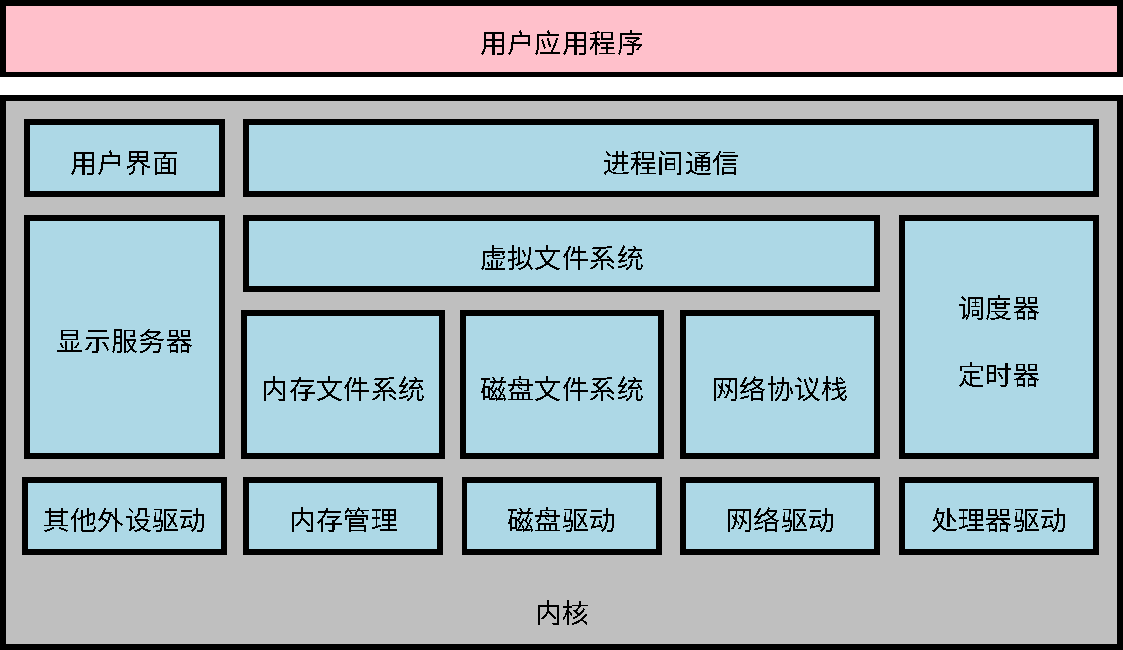
\includegraphics[width=0.72\textwidth]{Figure/image2.pdf}
    \caption{宏内核架构图}
    \label{fig:1-1-monolithic-kernel-architecture}
\end{figure}

\begin{figure}[htbp]
    \centering
    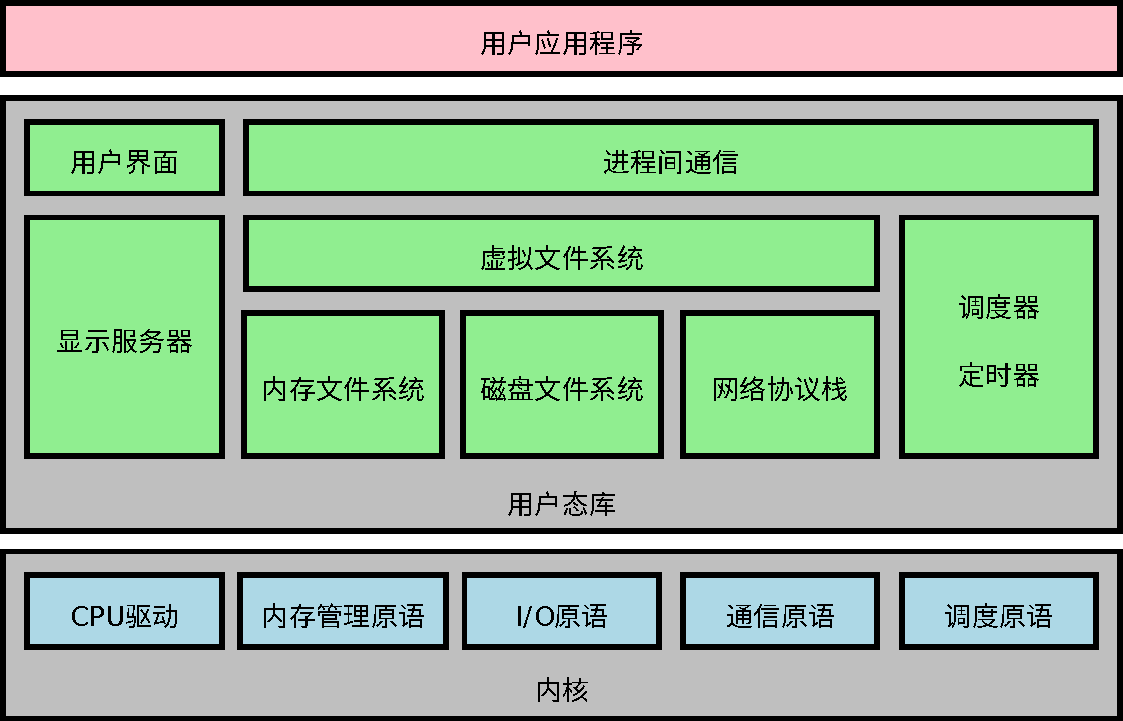
\includegraphics[width=0.72\textwidth]{Figure/image3.pdf}
    \caption{微内核架构图}
    \label{fig:1-2-microkernel-architecture}
\end{figure}

RME 采取的是微内核设计。一方面宏内核无需频繁跨保护域的优势在现代架构上已经很不明显\footnote{如最新 x86-64 的 SYSCALL 和 SYSRET 系统调用专用指令对仅消耗 60 周期，相当于一次三级缓存不命中}，另一方面微内核由于代码和数据的局部性极佳且内部结构简单而在缓存性能和并发性能上取得了决定性的优势，使得宏内核丧失了其唯一的优点------速度。新近开发的以 seL4\hyperref[cite:1-4]{{[}4{]}}为代表的一批微内核操作系统在进程间通信上可以好出 Linux 几十倍，其最坏响应时间视配置而定则要好出甚至更多。在应用程序性能上，基于微内核的网络功能虚拟化（Network
Function
Virtualization，NFV）应用也取得了普遍高出 Linux 一个数量级的性能，彻底否决了宏内核一定具有高性能的论断。

就 RME 本身而言，在某些单核架构\footnote{尤其是以 Cortex-M 为代表的一批微控制器}上的平均进程间通信性能是 Linux 的 40 倍；即便加上用户态库造成的开销，比 Linux 也要快出 25 倍。

\section{实时操作系统及其组件的性能指标}\label{sec:1-rtos-performance-metrics}

当前市场上有几百种不同种类的RTOS存在，而爱好者和个人开发的内核更是数不胜数。这些系统的性能往往是良莠不齐的。我们需要一些指标来衡量这些RTOS的性能。下面所列的指标都只能在处理器架构相同，编译器、编译选项相同的情况下进行直接比较。如果采用了不同的架构、编译器或编译选项，得到的数据没有直接意义，只具有参考性而不具有可比性。一个推荐的方法是使用工业实际标准的 ARM 或 MIPS 系列处理器配合 GCC-O2 选项进行评估。此外，也可以使用 Chronos 模拟器配合 GCC-O2 来进行评估。在评估时还要注意，系统的负载水平可能会对这些值有影响，因此只有在系统的负载水平一致的情况下，这些值才能够被比较。

\subsection{内核大小}\label{subsec:1-kernel-size}

内核的尺寸是衡量RTOS的一个重要指标。由于RTOS通常被部署在内存极度受限的设备中，因此内核的小体积是非常关键的。内核的尺寸主要从两个方面衡量，一是只读段大小，二是数据段大小。只读段包括了内核的代码段和只读数据段，数据段包括了内核的可读写数据段大小。在基于Flash的微控制器系统中，只读段会消耗Flash，而数据段则会消耗SRAM。\hyperref[cite:1-1]{{[}1{]}}

由于RTOS是高度可配置的，其内核大小往往不是固定的，而是和所选用的配置紧密相关的。因此，衡量此项性能，应该查看衡量最小内核配置、常见内核配置和最大内核配置下的内核大小。\hyperref[cite:1-1]{{[}1{]}}

内核大小数据的获得非常简单，只要用编译器编译该内核，然后使用专门的二进制查看器\footnote{如Objdump}查看目标文件各段的大小即可。

\subsection{执行时间、最坏执行时间及其抖动}\label{subsec:1-execution-time-and-jitter}

执行时间指RTOS系统调用的用时大小。最坏执行时间指执行时间在最不利条件下能达到的最大长度。RTOS的最坏执行时间通常会在如下情况下达到：执行耗时最长的系统调用，并在此过程中产生了大量的缓存未命中和快表未命中。RTOS在执行系统调用时一般都会关中断；最坏执行时间通常是系统关中断最长的时间，因此对系统的实时性的影响是非常巨大的。

最坏执行时间可以分成两类：第一类是内核系统调用的最坏执行时间，另一类是进程间通信和线程间同步的最坏执行时间。

要获得第一类最坏执行时间，可以在调用某个系统调用之前，计时器记下此时的时间戳T\textsubscript{s}，然后在系统调用结束之后，再调用计时器记下此时的时间戳T\textsubscript{e}。然后，连续调用两次计时器，记下两个时间戳T\textsubscript{ts}和T\textsubscript{te}，得到调用计时器的额外代价为T\textsubscript{te}-T\textsubscript{ts}。此时，执行时间就是T\textsubscript{e}-T\textsubscript{s}-(T\textsubscript{te}-T\textsubscript{ts})。最坏执行时间，就是所有的系统调用测试之中，执行时间最大的那一个。

要获得第二类最坏执行时间，可以在通信机制的发送端调用一次计时器，记下此时的时间戳T\textsubscript{s}，在通信机制的接收端调用一次计时器，记下此时的时间戳T\textsubscript{e}。对于调用计时器的代价测量是类似第一类最坏执行时间的。最终得到的T\textsubscript{e}-T\textsubscript{s}-(T\textsubscript{te}-T\textsubscript{ts})就是执行时间。最坏执行时间，就是所有的通信测试之中，执行时间最大的那一个。

执行时间的抖动也是非常重要的。在多次测量同一个系统的执行、通信时间时，我们往往会得到一个分布。这个分布的平均值是平均执行时间，其标准差\footnote{有时我们也使用极差}被称为执行时间抖动。

对于一个RTOS，我们通常认为执行时间、最坏执行时间和抖动都是越小越好。执行时间又可以详细分成以下几类：\hyperref[cite:1-1]{{[}1{]}}

\subsubsection{进程内线程切换时间}\label{subsubsec:1-intra-process-thread-switch}

进程内线程切换时间指在同一个进程内从一个线程切换到另外一个线程所消耗的时间。我们用下图的方法进行测量。在测量时，除了使用T\textsubscript{e}-T\textsubscript{s}的方法，也可以使用两次T\textsubscript{s}之间的差值除以2。线程切换包括两种情况，一种情况是同优先级线程之间互相切换，另外一种是由低优先级线程唤醒高优先级线程。\hyperref[cite:1-2]{{[}2{]}}

在第一种情况下，我们假设图中的两个线程是相同优先级的，而且在测量开始时，我们正执行的是刚刚由线程B切换过来的线程A。

\begin{xltabular}{\textwidth}{@{}>{\hsize=1.0000\hsize\raggedright\arraybackslash}X>{\hsize=1.0000\hsize\raggedright\arraybackslash}X@{}}
\caption{进程内线程切换的第一种情况}\label{tab:1-1-intra-process-thread-switch-case-1}\\
\toprule
进程1：线程A & 进程1：线程B\tabularnewline
\endfirsthead
\toprule
进程1：线程A & 进程1：线程B\tabularnewline
\midrule
\endhead
\bottomrule
\endlastfoot
永久循环

\{

\textgreater\textgreater{} 计时T\textsubscript{s}；

切换到线程B；

\}\strut
 & 永久循环

\{

计时T\textsubscript{e}；

\textgreater\textgreater{} 切换到线程A；

\}\strut
\tabularnewline
\end{xltabular}

在第二种情况下，我们假设图中的线程B优先级较高，而且在测量开始时，我们正执行的是刚刚由线程B切换过来的线程A。

\begin{xltabular}{\textwidth}{@{}>{\hsize=1.0045\hsize\raggedright\arraybackslash}X>{\hsize=0.9955\hsize\raggedright\arraybackslash}X@{}}
\caption{进程内线程切换的第二种情况}\label{tab:1-2-intra-process-thread-switch-case-2}\\
\toprule
进程1：线程A & 进程1：线程B\tabularnewline
\endfirsthead
\toprule
进程1：线程A & 进程1：线程B\tabularnewline
\midrule
\endhead
\bottomrule
\endlastfoot
永久循环

\{

\textgreater\textgreater{} 计时T\textsubscript{s}；

唤醒B（传统）或切换到B（微内核）；

\}\strut
 & 永久循环

\{

计时T\textsubscript{e}；

\textgreater\textgreater{} 睡眠（传统）或切换到A（微内核）；

\}\strut
\tabularnewline
\end{xltabular}

\subsubsection{进程间线程切换时间}\label{subsubsec:1-inter-process-thread-switch}

进程间线程切换时间指在不同进程间从一个线程切换到另外一个线程所消耗的时间。测量方法和两种可能情况与上节所述是完全一致的，唯一的区别是现在参与测试的线程属于两个进程。\hyperref[cite:1-2]{{[}2{]}}

在第一种情况下，我们假设图中的两个线程是相同优先级的，而且在测量开始时，我们正执行的是

刚刚由线程B切换过来的线程A。

\begin{xltabular}{\textwidth}{@{}>{\hsize=1.0000\hsize\raggedright\arraybackslash}X>{\hsize=1.0000\hsize\raggedright\arraybackslash}X@{}}
\caption{进程间线程切换的第一种情况}\label{tab:1-3-inter-process-thread-switch-case-1}\\
\toprule
进程1：线程A & 进程2：线程B\tabularnewline
\endfirsthead
\toprule
进程1：线程A & 进程2：线程B\tabularnewline
\midrule
\endhead
\bottomrule
\endlastfoot
永久循环

\{

\textgreater\textgreater{} 计时T\textsubscript{s}；

切换到线程B；

\}\strut
 & 永久循环

\{

计时T\textsubscript{e}；

\textgreater\textgreater{} 切换到线程A；

\}\strut
\tabularnewline
\end{xltabular}

在第二种情况下，我们假设图中的线程B优先级较高，而且在测量开始时，我们正执行的是刚刚由线程B切换过来的线程A。

\begin{xltabular}{\textwidth}{@{}>{\hsize=1.0044\hsize\raggedright\arraybackslash}X>{\hsize=0.9956\hsize\raggedright\arraybackslash}X@{}}
\caption{进程间线程切换的第二种情况}\label{tab:1-4-inter-process-thread-switch-case-2}\\
\toprule
进程1：线程A & 进程2：线程B\tabularnewline
\endfirsthead
\toprule
进程1：线程A & 进程2：线程B\tabularnewline
\midrule
\endhead
\bottomrule
\endlastfoot
永久循环

\{

\textgreater\textgreater{} 计时T\textsubscript{s}；

唤醒B（传统）或切换到B（微内核）；

\}\strut
 & 永久循环

\{

计时T\textsubscript{e}；

\textgreater\textgreater{} 睡眠（传统）或切换到A（微内核）；

\}\strut
\tabularnewline
\end{xltabular}

\subsubsection{进程内线程间同步通信时间}\label{subsubsec:1-intra-process-sync-communication}

进程内线程间同步通信时间指在同一个进程内不同线程之间进行同步通信所用的总时间。以下测量假设线程B已经在接收端阻塞，线程A进行发送，而且线程B的优先级比线程A高。对于使用线程迁移技术进行通信的系统\footnote{比如RME和部分L4系列}，此参数的测量没有意义，因为进程内不需要使用同步通信。\hyperref[cite:1-2]{{[}2{]}}

\begin{xltabular}{\textwidth}{@{}>{\hsize=1.0000\hsize\raggedright\arraybackslash}X>{\hsize=1.0000\hsize\raggedright\arraybackslash}X@{}}
\caption{进程内线程间同步通信}\label{tab:1-5-intra-process-sync-communication}\\
\toprule
进程1：线程A & 进程1：线程B\tabularnewline
\endfirsthead
\toprule
进程1：线程A & 进程1：线程B\tabularnewline
\midrule
\endhead
\bottomrule
\endlastfoot
永久循环

\{

\textgreater\textgreater{} 计时T\textsubscript{s}；

向同步端点P发送信号；

\}\strut
 & 永久循环

\{

计时T\textsubscript{e}；

\textgreater\textgreater{} 从同步端点P接收信号；

\}\strut
\tabularnewline
\end{xltabular}

\subsubsection{进程间同步通信时间}\label{subsubsec:1-inter-process-sync-communication}

进程间同步通信时间指在不同进程间进行同步通信所用的总时间。以下测量适用于传统操作系统，并假设线程B已经在接收端阻塞，线程A进行发送，而且线程B的优先级比线程A高。\hyperref[cite:1-2]{{[}2{]}}

\begin{xltabular}{\textwidth}{@{}>{\hsize=1.0000\hsize\raggedright\arraybackslash}X>{\hsize=1.0000\hsize\raggedright\arraybackslash}X@{}}
\caption{传统操作系统的进程间同步通信}\label{tab:1-6-inter-process-sync-communication}\\
\toprule
进程1：线程A & 进程2：线程B\tabularnewline
\endfirsthead
\toprule
进程1：线程A & 进程2：线程B\tabularnewline
\midrule
\endhead
\bottomrule
\endlastfoot
永久循环

\{

\textgreater\textgreater{} 计时T\textsubscript{s}；

向同步端点P发送信号；

\}\strut
 & 永久循环

\{

计时T\textsubscript{e}；

\textgreater\textgreater{} 从同步端点P接收信号；

\}\strut
\tabularnewline
\end{xltabular}

对于 RME 和 L4 一类采用了线程迁移技术的操作系统，其测量如下。注意，当线程A迁移调用了函数F的时候，我们仍然在线程A内部运行，只不过所执行的代码段和所使用的数据段跑到了另外一个进程内部，并且在该进程内部使用了一个另外分配的执行栈。

\begin{xltabular}{\textwidth}{@{}>{\hsize=1.0994\hsize\raggedright\arraybackslash}X>{\hsize=0.9006\hsize\raggedright\arraybackslash}X@{}}
\caption{线程迁移技术的进程间同步通信}\label{tab:1-7-thread-migration-sync-communication}\\
\toprule
进程1：线程A & 进程2：线程A\tabularnewline
\endfirsthead
\toprule
进程1：线程A & 进程2：线程A\tabularnewline
\midrule
\endhead
\bottomrule
\endlastfoot
永久循环

\{

\textgreater\textgreater{} 计时T\textsubscript{s}；

迁移调用函数F；

\}\strut
 & 函数F

\{

计时T\textsubscript{e}；

返回；

\}\strut
\tabularnewline
\end{xltabular}

\subsubsection{线程内异步通信时间}\label{subsubsec:1-intra-thread-async-communication}

线程内异步通信时间指在同一个线程内发送和接收异步信号所用的总时间。常见的异步信号可以包括 RME 系统所提供的异步信号原语（Signal），或者其他操作系统提供的信号量（Semaphore），邮箱（Mailbox），消息队列（Queue）、管道（Pipe）、等等。我们用下图的方法进行测量。\hyperref[cite:1-2]{{[}2{]}}
最终的测量结果中，T\textsubscript{i}-T\textsubscript{s}得到的是发送所消耗的时间，T\textsubscript{e}-T\textsubscript{i}得到的是接收所消耗的时间，T\textsubscript{e}-T\textsubscript{i}则是通信用时。

\begin{xltabular}{\textwidth}{@{}>{\hsize=1.0000\hsize\raggedright\arraybackslash}X@{}}
\caption{线程内异步通信}\label{tab:1-8-intra-thread-async-communication}\\
\toprule
线程A\tabularnewline
\endfirsthead
\toprule
线程A\tabularnewline
\midrule
\endhead
\bottomrule
\endlastfoot
永久循环

\{

计时T\textsubscript{s}；

向异步端点P发送信号；

计时T\textsubscript{i}；

从异步端点P接收信号；

计时T\textsubscript{e}；

\}\strut
\tabularnewline
\end{xltabular}

\subsubsection{进程内线程间异步通信时间}\label{subsubsec:1-intra-process-async-communication}

进程内线程间异步通信时间指在同一个进程内的不同线程之间发送和接收异步信号所用的总时间。我们用下图的方法进行测量。我们假设线程B已经在接收端阻塞，线程A进行发送，而且线程B的优先级比线程A高。\hyperref[cite:1-2]{{[}2{]}}

\begin{xltabular}{\textwidth}{@{}>{\hsize=1.0000\hsize\raggedright\arraybackslash}X>{\hsize=1.0000\hsize\raggedright\arraybackslash}X@{}}
\caption{进程内线程间异步通信}\label{tab:1-9-intra-process-async-communication}\\
\toprule
进程1：线程A & 进程1：线程B\tabularnewline
\endfirsthead
\toprule
进程1：线程A & 进程1：线程B\tabularnewline
\midrule
\endhead
\bottomrule
\endlastfoot
永久循环

\{

\textgreater\textgreater{} 计时T\textsubscript{s}；

向异步端点P发送信号；

\}\strut
 & 永久循环

\{

计时T\textsubscript{e}；

\textgreater\textgreater{} 从异步端点P接收信号；

\}\strut
\tabularnewline
\end{xltabular}

\subsubsection{进程间异步通信时间}\label{subsubsec:1-inter-process-async-communication}

进程间异步通信时间指在不同进程间发送和接收异步信号所用的总时间。测量方法和上节所述是完全一致的，唯一的区别是现在参与测试的线程属于两个进程。\hyperref[cite:1-2]{{[}2{]}}

\begin{xltabular}{\textwidth}{@{}>{\hsize=1.0000\hsize\raggedright\arraybackslash}X>{\hsize=1.0000\hsize\raggedright\arraybackslash}X@{}}
\caption{进程间异步通信}\label{tab:1-10-inter-process-async-communication}\\
\toprule
进程1：线程A & 进程2：线程B\tabularnewline
\endfirsthead
\toprule
进程1：线程A & 进程2：线程B\tabularnewline
\midrule
\endhead
\bottomrule
\endlastfoot
永久循环

\{

\textgreater\textgreater{} 计时T\textsubscript{s}；

向异步端点P发送信号；

\}\strut
 & 永久循环

\{

计时T\textsubscript{e}；

\textgreater\textgreater{} 从异步端点P接收信号；

\}\strut
\tabularnewline
\end{xltabular}

\subsubsection{页表操作时间}\label{subsubsec:1-page-table-operation-time}

页表操作时间指操作页表项所用的时间。由于不同的操作系统提供的功能层级和复杂程度在这方面差异很大，因此不能简单地进行对比。通常地，一个微内核会提供能够对底层页表进行直接构造和映射的系统调用，而一个宏内核则会提供映射页到进程空间的操作。一些使用于微控制器上的内核则采用固定块分配的操作。总的而言，对这类操作的计时方法非常简单，就是在调用此类系统调用时进行计时，然后在调用结束后再次计时即可。\hyperref[cite:1-1]{{[}1{]}}\hyperref[cite:1-2]{{[}2{]}}

\begin{xltabular}{\textwidth}{@{}>{\hsize=1.0000\hsize\raggedright\arraybackslash}X@{}}
\caption{页表操作}\label{tab:1-11-page-table-operations}\\
\toprule
线程A\tabularnewline
\endfirsthead
\toprule
线程A\tabularnewline
\midrule
\endhead
\bottomrule
\endlastfoot
永久循环

\{

计时T\textsubscript{s}；

进行该操作；

计时T\textsubscript{e}；

\}\strut
\tabularnewline
\end{xltabular}

\subsection{中断响应时间、最坏中断响应时间及其抖动}\label{subsec:1-interrupt-response-time-and-jitter}

中断响应时间指从中断发生到RTOS调用中断对应的处理线程之间的时间。最坏中断响应时间指中断响应时间在最不利条件下能达到的最大长度。最坏中断响应时间通常会在如下情况下达到：在中断处理过程中发生了大量的缓存未命中和快表未命中。中断响应时间是RTOS最重要的指标，甚至可以说，RTOS的一切设计都是围绕着该指标进行的。该指标是RTOS对外界刺激响应时间的最直接的标准。

要获得最坏中断响应时间，可以在中断向量的第一行汇编代码\footnote{不能等到 C 函数中再去调用，因为寄存器和堆栈维护也是中断响应时间的一部分}中调用计时器，得到一个时间戳T\textsubscript{s}；在中断处理线程的第一行代码处调用计时器，得到一个时间戳T\textsubscript{e}。对于计时器代价的测量同上。最终得到的T\textsubscript{e}-T\textsubscript{s}-(T\textsubscript{te}-T\textsubscript{ts})就是中断响应时间。最坏中断响应时间，就是所有的中断响应测试之中，响应时间最大的那一个。

中断响应时间的抖动也是非常重要的。在多次测量同一个系统的中断响应时间时，我们往往会得到一个分布。这个分布的平均值是平均中断响应时间，其标准差\footnote{有时我们也使用极差}被称为中断响应时间抖动。

\needspace{20\baselineskip}
对于一个RTOS，我们通常认为中断响应时间、最坏中断响应时间和抖动都是越小越好。中断响应时间的测量通常如下所示\hyperref[cite:1-1]{{[}1{]}}\hyperref[cite:1-3]{{[}3{]}}：

\begin{xltabular}{\textwidth}{@{}>{\hsize=1.0512\hsize\raggedright\arraybackslash}X>{\hsize=0.9488\hsize\raggedright\arraybackslash}X@{}}
\caption{中断响应时间}\label{tab:1-12-interrupt-response-time}\\
\toprule
内核 & 线程A\tabularnewline
\endfirsthead
\toprule
内核 & 线程A\tabularnewline
\midrule
\endhead
\bottomrule
\endlastfoot
硬件中断向量

\{

\textgreater\textgreater{} 计时T\textsubscript{s}；

从内核向异步端点P发送信号；

\}\strut
 & 永久循环

\{

计时T\textsubscript{e}；

\textgreater\textgreater{} 从异步端点P接收信号；

\}\strut
\tabularnewline
\end{xltabular}

\subsection{实际中断响应时间、最坏实际中断响应时间及其抖动}\label{subsec:1-actual-interrupt-response-time-and-jitter}

实际中断响应时间指软硬件系统从中断外部信号输入到发出IO操作响应之间的时间。最坏实际中断响应时间指实际中断响应时间在最不利条件下能达到的最大长度。影响实际最坏中断响应时间的因素中，除了那些能影响最坏中断响应时间的因素之外，还有对应的CPU及IO硬件本身的因素。

要获得实际中断响应时间，我们需要一些外部硬件来支持该种测量。比如，我们需要测量某系统的I/O的实际中断响应时间，我们可以将一个FPGA的管脚连接到某CPU或主板的输入管脚，然后将另一个管脚连接到某CPU或者主板上的输出管脚。首先，FPGA向输入管脚发出一个信号，此时FPGA内部的高精度计时器开始工作；在FPGA接收到输出管脚上的信号的时候，FPGA内部的高精度计时器停止工作。最终得到的FPGA内部计时器的时间就是系统的实际中断响应时间。最坏实际中断响应时间，就是所有测试之中，响应时间最大的那一个。

对于一个软硬件系统，我们通常认为实际中断响应时间、最坏实际中断响应时间和抖动都是越小越好。值得注意的是，实际中断响应时间一般会大约等于最坏执行时间加上最坏中断响应时间加上系统CPU/IO的固有延迟。比如，某系统在IO输入来临时刚刚开始执行某系统调用，此时硬件中断向量无法立刻得到执行，必须等到该系统调用执行完毕才可以。等到该系统调用执行完毕时，实际的硬件中断向量才开始执行，切换到处理线程进行处理并产生输出。实际中断响应时间的测量通常如下所示\hyperref[cite:1-1]{{[}1{]}}：

\begin{xltabular}{\textwidth}{@{}>{\hsize=0.9656\hsize\raggedright\arraybackslash}X>{\hsize=1.0344\hsize\raggedright\arraybackslash}X@{}}
\caption{实际中断响应时间}\label{tab:1-13-actual-interrupt-response-time}\\
\toprule
FPGA（或者示波器） & 被测系统\tabularnewline
\endfirsthead
\toprule
FPGA（或者示波器） & 被测系统\tabularnewline
\midrule
\endhead
\bottomrule
\endlastfoot
永久循环

\{

\textgreater\textgreater{} 发出信号并启动计时器；

接收信号；

停止计时器；

\}\strut
 & 永久循环

\{

从I/O上接收信号；

最简化的内部处理流程；

从I/O上输出信号；

\}\strut
\tabularnewline
\end{xltabular}

\subsection{输入输出性能指标}\label{subsec:1-io-performance-metrics}

I/O性能指标主要适用于那些提供了I/O子系统的操作系统，尤其是那些提供了虚拟化支持的操作系统。常见的I/O子系统有磁盘系统、网络系统、串并行端口系统和各种采集卡系统等；在微控制器上，它更多地表现为GPIO、PWM发生器和LCD控制器等等。对众多I/O子系统的评价标准往往各有不同，但是通常它们都包括两个部分：吞吐量和延迟。吞吐量指的是系统在某段时间之内能达到的I/O系统数据传输率，延迟指的是系统从发出I/O请求到得到回应所需的时间。

\subsection{虚拟化性能指标}\label{subsec:1-virtualization-performance-metrics}

对于那些支持虚拟化\footnote{包括全虚拟化和准虚拟化}其他操作系统的操作系统\footnote{如 RME，NOVA\hyperref[cite:1-5]{{[}5{]}} 和部分 L4}，对虚拟化性能指标的评价也是非常重要的。虚拟化性能指标一般包括两个部分，一个是虚拟机功能部分，还有一个是虚拟机性能部分。此外，虚拟机之间的通信开销也是一个重要的指标。

在虚拟机功能方面，我们一般会评估虚拟机的各项功能是否都被正确实现和支持。正确实现和支持的功能越多，功能指标就越好。

在虚拟机性能部分的评估中，要评估的虚拟机性能指标和\ref{subsec:1-execution-time-and-jitter}
列出的种种指标是一样的。此外，还要衡量虚拟化引入的额外性能消耗和存储资源消耗。虚拟化所引起的额外性能消耗越少，存储资源消耗越少，那么虚拟化的性能指标就越好。

虚拟机之间的通信开销也是一个非常重要的话题。虚拟机之间的通信开销一般都会比虚拟机内部的通信开销大，并且往往会通过专用的驱动或虚拟网络来支持。虚拟机之间通信开销的测量和I/O性能的测量方法是一致的，在此也不赘述。

\section{RME系统调用格式}\label{sec:1-system-call-format}

系统调用是使用系统提供的功能的唯一方法。对于 RME，这是使用其系统功能的唯一方法。通常而言，系统调用都通过软中断\footnote{比如ARM的SWI、SVC}实现，也可以通过专用的系统调用指令实现\footnote{比如x86-64的SYSCALL/SYSRET}。对于软中断方法实现，一旦调用了软中断指令，系统即跳转到软中断处理向量，进行中断处理。系统调用的参数会通过某种手段\footnote{一般是共享内存或者寄存器}传递到内核，然后由内核进行调用处理。对于专用指令实现，内核会切换到事先设置好的内核栈，并且直接跳转到系统调用处理函数的入口，参数传递则是与软中断实现一样的。

RME 同时支持两种方法。在 x86-64 架构上我们采用后者，而在 ARM 架构上我们采用前者。

\subsection{系统调用基本方法}\label{subsec:1-system-call-basics}

RME 系统调用的基本方法是，先把四个机器字长的参数依次放入四个寄存器，然后调用软中断指令或者专用内核调用指令。RME 在任何架构上都总是使用四个寄存器来传递参数，因为这是目前大多数CPU架构的 C 语言函数调用约定中，允许的不通过栈传递的最多参数数量\footnote{比如MIPS和ARM均为前四个参数通过寄存器传递，后面的参数通过栈传递}。

RME 所有的系统调用都不会使用超过4个寄存器长度的参数。此外，RME 也不通过内存来传递参数\footnote{Linux、早期的某些L4系统会这样做}。通过内存传递参数可能导致在内核态对用户态指针解引用，从而导致内核态的内存段错误，这往往很难处理，而且有几率造成内核崩溃或权限盗用。

\subsection{参数传递与参数位置编码}\label{subsec:1-parameter-passing-and-encoding}

\needspace{24\baselineskip}
RME 系统调用的参数被放在寄存器内传递。但是，某些寄存器的长度超过了我们要传递的参数的长度，因此使用一个寄存器仅仅传递一个参数太过奢侈，我们可以传递更多的参数。因此，我们把寄存器切成多段使用。在 RME 中，我们最多会把一个寄存器切成8段来使用。以32位系统为例，其各段的定义和标识符如下图所示\footnote{此处以32位机器为例；64位机器依此类推}：

\needspace{14\baselineskip}
\begin{xltabular}{\textwidth}{@{}*{8}{>{\centering\arraybackslash}X}@{}}
\caption{系统调用参数位置编码}\label{tab:1-14-system-call-parameter-encoding}\\
\toprule
\multicolumn{8}{c}{[31 \quad 32 位机器字 \quad 0]}\\
\midrule
\multicolumn{4}{c}{\makecell{D1\\31--16}} & \multicolumn{4}{c}{\makecell{D0\\15--0}}\\
\midrule
\multicolumn{2}{c}{\makecell{Q3\\31--24}} & \multicolumn{2}{c}{\makecell{Q2\\23--16}} & \multicolumn{2}{c}{\makecell{Q1\\15--8}} & \multicolumn{2}{c}{\makecell{Q0\\7--0}}\\
\midrule
\makecell{O7\\31--28} & \makecell{O6\\27--24} & \makecell{O5\\23--20} & \makecell{O4\\19--16} & \makecell{O3\\15--12} & \makecell{O2\\11--8} & \makecell{O1\\7--4} & \makecell{O0\\3--0}\\
\bottomrule
\end{xltabular}

{\small\noindent D、Q、O 分别表示把 32 位机器字等分为 2 段、4 段和 8 段时的段编号；每行单元格的宽度对应其实际位宽。\par}

RME 也有少数特殊的系统调用使用其他的值传递方法。这些方法会在相关的函数处加以具体说明。

\subsubsection{系统调用号}\label{subsubsec:1-system-call-number}

系统调用号指明了系统调用的编号。这个编号总是位于第一个寄存器（P0）的 D1 位置，我们也把它记作 N。RME 一共有 0-33 共 34 个系统调用，分别如下：

\begin{xltabular}{\textwidth}{@{}>{\hsize=1.0292\hsize\raggedright\arraybackslash}X>{\hsize=0.6509\hsize\raggedright\arraybackslash}X>{\hsize=1.3198\hsize\raggedright\arraybackslash}X@{}}
\caption{RME系统调用一览}\label{tab:1-15-system-call-list}\\
\toprule
系统调用名称 & 调用号 & 意义\tabularnewline
\endfirsthead
\toprule
系统调用名称 & 调用号 & 意义\tabularnewline
\midrule
\endhead
\bottomrule
\endlastfoot
RME\_SVC\_INV\_RET & 0 & 从迁移调用返回\tabularnewline
RME\_SVC\_INV\_ACT & 1 & 进行迁移调用\tabularnewline
RME\_SVC\_SIG\_SND & 2 & 向信号端点发送信号\tabularnewline
RME\_SVC\_SIG\_RCV & 3 & 从信号端点接收信号\tabularnewline
RME\_SVC\_KFN & 4 & 进行内核特殊功能函数调用\tabularnewline
RME\_SVC\_THD\_SCHED\_FREE & 5 & 将某线程从某个CPU上释放\tabularnewline
RME\_SVC\_THD\_EXEC\_SET & 6 &
设置线程的执行属性\footnote{入口和栈}\tabularnewline
RME\_SVC\_THD\_SCHED\_PRIO & 7 & 更改某线程的优先级\tabularnewline
RME\_SVC\_THD\_TIME\_XFER & 8 & 在线程间传递时间片\tabularnewline
RME\_SVC\_THD\_SWT & 9 & 切换到某线程\tabularnewline
RME\_SVC\_CPT\_CRT & 10 & 创建一个权能表\tabularnewline
RME\_SVC\_CPT\_DEL & 11 & 删除一个权能表\tabularnewline
RME\_SVC\_CPT\_FRZ & 12 & 冻结权能表内的某权能\tabularnewline
RME\_SVC\_CPT\_ADD & 13 & 进行权能传递\tabularnewline
RME\_SVC\_CPT\_REM & 14 & 移除权能表内的某权能\tabularnewline
RME\_SVC\_PGT\_CRT & 15 & 创建一个页目录\tabularnewline
RME\_SVC\_PGT\_DEL & 16 & 删除一个页目录\tabularnewline
RME\_SVC\_PGT\_ADD & 17 & 添加一个页表项\tabularnewline
RME\_SVC\_PGT\_REM & 18 & 移除一个页表项\tabularnewline
RME\_SVC\_PGT\_CON & 19 & 构造页表\tabularnewline
RME\_SVC\_PGT\_DES & 20 & 析构页表\tabularnewline
RME\_SVC\_PRC\_CRT & 21 & 创建一个进程\tabularnewline
RME\_SVC\_PRC\_DEL & 22 & 删除一个进程\tabularnewline
RME\_SVC\_PRC\_CPT & 23 & 替换进程的权能表\tabularnewline
RME\_SVC\_PRC\_PGT & 24 & 替换进程的页表\tabularnewline
RME\_SVC\_THD\_CRT & 25 & 创建一个线程\tabularnewline
RME\_SVC\_THD\_DEL & 26 & 删除一个线程\tabularnewline
RME\_SVC\_THD\_SCHED\_BIND & 27 & 将线程绑定到某处理器\tabularnewline
RME\_SVC\_THD\_SCHED\_RCV & 28 & 接收某线程的调度器信息\tabularnewline
RME\_SVC\_SIG\_CRT & 29 & 创建一个信号端点\tabularnewline
RME\_SVC\_SIG\_DEL & 30 & 删除一个信号端点\tabularnewline
RME\_SVC\_INV\_CRT & 31 & 创建一个迁移调用\tabularnewline
RME\_SVC\_INV\_DEL & 32 & 删除一个迁移调用\tabularnewline
RME\_SVC\_INV\_SET & 33 &
设置迁移调用的执行属性\footnote{入口和栈}\tabularnewline
保留 & 34-63 & 暂时不使用，为未来保留\tabularnewline
\end{xltabular}

\subsubsection{权能表权能号}\label{subsubsec:1-capability-table-number}

权能表权能号指明了要操作的权能表。这个编号总是位于第一个寄存器 P0 的 D0 位置，我们把它记作 C。由于只有部分操作需要用到权能表权能，因此只有在此时这个位置上的值才有意义。

\subsubsection{其他参数}\label{subsubsec:1-other-parameters}

第一个参数在第二个寄存器中进行传递，第二个参数在第三个寄存器中传递，第三个参数在第四个寄存器中传递。我们把这些参数分别记作 P1、P2 和 P3。在系统调用文档中，P1.D1 表示 P1 的 D1 部分，依此类推。

\subsection{特殊说明}\label{subsec:1-special-notes}

\begin{enumerate}
\def\labelenumi{\arabic{enumi}.}
\item
  在创建内核对象时，内核虚拟地址必须对齐于 2 的 RME\_KOM\_SLOT\_ORDER 次方。
\item
  系统调用号0-8可能导致潜在的线程切换，为了单独优化，它们被分配了连续的调用号。
\item
  所有的系统调用成功时的返回值均为非负值，失败后的返回值均为负值。
\item
  在本手册中，所有的 typedef 类型的前缀``rme\_''都被省略来节约表格空间。
\end{enumerate}

\section{手册总览}\label{sec:1-manual-overview}

在接下来的各个章节中，我们将分别介绍 RME 的各个子系统。其中\hyperref[sec:2-capability-concept]{第2章}
介绍权能表和权能管理，\hyperref[sec:3-memory-management-overview]{第3章}
介绍页表和内存管理，\hyperref[sec:4-process-and-thread-overview]{第4章}
介绍进程和线程管理，\hyperref[sec:5-sync-async-overview]{第5章}
介绍同步通信机制和异步通信机制，\hyperref[sec:6-kernel-call-overview]{第6章}
介绍内核功能调用机制。之后，我们会在\hyperref[sec:7-porting-overview]{第7章}
介绍 RME 的移植方法，以及在\hyperref[sec:8-kernel-call-implementation-overview]{第8章}
介绍 RME 中内核调用功能的实现标准。最后，我们会在\hyperref[sec:9-special-kernel-features]{第9章}
介绍 RME 中存在的一些已知问题及其解决方案。

在本技术参考手册中介绍的仅仅是RME的内核本身。关于各个架构上RME的具体实现细节，请参看对应架构的架构手册；关于RME用户态库的信息，请参看RME的用户态库\footnote{也即 RVM（M7M2）}使用手册。

本手册假定读者对操作系统的基本概念有一般了解。有关微内核和 RME 的较为艰深的概念在各章的开头会分别加以介绍。

\section{RME架构总览}\label{sec:1-architecture-overview}

下图是一张横置的简略架构总览图。图中除了包括 RME 的内核本身，还包括了其用户态库，以及其用户态库中的各种组件。图中的黑虚线方框代表逻辑独立的软件模组，黑实线方框代表硬件保护隔离的软件模组，灰实线方框则代表软件包的边界，含有省略号（......）的方框则代表了与左侧紧邻方框相同内容因而被省略的子系统。由于篇幅有限，因此图中仅展示出相对重要的组件，有部分组件并未展示出来；关于详细的用户态架构图，请参看RME的用户态库使用手册。

\begin{figure}[htbp]
    \centering
    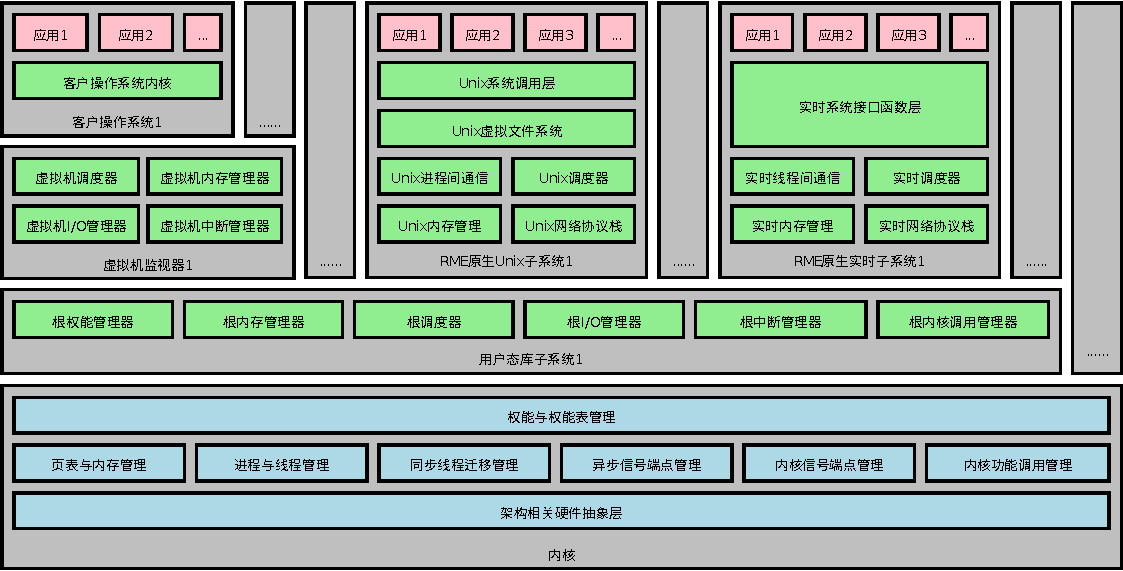
\includegraphics[width=0.90\textwidth]{Figure/image4.pdf}
    \caption{RME简略架构总览}
    \label{fig:1-3-rme-architecture-overview}
\end{figure}

\section{本章参考文献}\label{sec:1-bibliography}

\protect\phantomsection\label{cite:1-1}

\noindent {[}1{]} T. N. B. Anh and S.-L. Tan, ``Real-time operating systems for small microcontrollers,'' \textit{IEEE Micro}, vol. 29, 2009.

\protect\phantomsection\label{cite:1-2}

\noindent {[}2{]} R. P. Kar, ``Implementing the Rhealstone real-time benchmark,'' \textit{Dr. Dobb's Journal}, vol. 15, pp. 46--55, 1990.

\protect\phantomsection\label{cite:1-3}

\noindent {[}3{]} T. J. Boger, ``Rhealstone benchmarking of FreeRTOS and the Xilinx Zynq extensible processing platform,'' M.S. thesis, Temple University, 2013.

\protect\phantomsection\label{cite:1-4}

\noindent {[}4{]} G. Klein, K. Elphinstone, G. Heiser, J. Andronick, D. Cock, P. Derrin, et al., ``seL4: formal verification of an OS kernel,'' in \textit{Proceedings of the ACM SIGOPS 22nd Symposium on Operating Systems Principles}, Big Sky, MT, USA, 2009.

\protect\phantomsection\label{cite:1-5}

\noindent {[}5{]} U. Steinberg and B. Kauer, ``NOVA: a microhypervisor-based secure virtualization architecture,'' in \textit{Proceedings of the 5th European Conference on Computer Systems}, 2010, pp. 209--222.


\chapter{权能表和权能管理}\label{ch:capability-table-management}

\section{权能的概念}\label{sec:2-capability-concept}

权能（Capability）是一种最早在多用户计算机系统中引入的用来控制访问权限的凭证\hyperref[cite:2-1]{{[}1{]}}。它是一种不可伪造的用来唯一标识某种资源以及允许对该资源所进行的操作的凭证。比如，Unix 的文件描述符就是一种权能\hyperref[cite:2-2]{{[}2{]}}；Windows 的访问权限也是一种权能。从某种意义上讲，权能就是一个指向某种资源的胖指针（Fat
Pointer）。

我们使用如下三条原则来保证系统的安全性\hyperref[cite:2-2]{{[}2{]}}：

\begin{enumerate}
\def\labelenumi{\arabic{enumi}.}
\item
  权能是不可伪造和不可在用户态擅自修改的；
\item
  进程只能用良好定义的授权接口获取权能；
\item
  权能只会被给予那些系统设计时负责管理该资源的进程。

  第三代微内核普遍采用权能的概念来管理资源。在 RME 中，所有的内核资源都是使用权能来管理的，并且权能全部位于内核空间中的权能表内。每个进程都对应一个权能表（Capability
  Table），在调用系统调用时，系统查找内核对象就是从该进程的权能表内查找的。每个权能都有一系列的操作标志位，如果某个权能拥有某个操作标志位，那么就可以通过这个权能对该内核对象做此种操作\hyperref[cite:2-3]{{[}3{]}}。绝大多数系统，如 seL4 等\hyperref[cite:2-5]{{[}5{]}}，都具有操作标志位。但是对于一些其他系统\footnote{如Composite等}，某种内核对象的操作只有一个，因此不需要单独的操作标志位\hyperref[cite:2-4]{{[}4{]}}。

  除了权能之外，还有另外一种称为访问控制列表（Access Control List，ACL）\hyperref[cite:2-6]{{[}6{]}}的方法。它也可以用来管理权限，但是其访问权限管理粒度较粗，而且表格很容易变得很大。它的优点是权能的授予和撤销相对简单\footnote{尤其是撤销操作}。

  在 RME 中，使用权能的概念，可以方便地实现自主访问控制（Discretionary Access
  Control，DAC）和强制访问控制（Mandatory Access
  Control，MAC），也能方便地构建起多级安全机制，并且根据最小特权的原则规划整个用户应用程序的设计。
\end{enumerate}

\section{权能表的操作和权能的状态}\label{sec:2-capability-table-operations-and-states}

权能表是一种用来存放权能的内核对象。在 RME 中它是一个线性数组，每个数组位置的大小都是固定的8个机器字，可以用来存放一个权能。在权能内部，记载着内核资源的确切类型、在内核内存中的确切位置\footnote{一个指向内核地址空间的指针}、权能的父权能、权能传递引用计数和权能的当前状态。此外，还有一个时间戳计数器用来在多核并行情况下用来保证权能的操作安定（Quiescence）。

\subsection{权能的类型}\label{subsec:2-capability-types}

在 RME 中，权能一共有8种类型\footnote{不包括空白权能}，如下表所示。关于相应类型权能的信息，请查看相应的章节作为参考。本章只讲述权能表权能相关的内容。

\begin{xltabular}{\textwidth}{@{}>{\hsize=0.8412\hsize\raggedright\arraybackslash}X>{\hsize=0.7467\hsize\raggedright\arraybackslash}X>{\hsize=1.4121\hsize\raggedright\arraybackslash}X@{}}
\caption{权能的类型}\label{tab:2-1-capability-types}\\
\toprule
权能类型号 & 权能类型 & 用途\tabularnewline
\endfirsthead
\toprule
权能类型号 & 权能类型 & 用途\tabularnewline
\midrule
\endhead
\bottomrule
\endlastfoot
RME\_CAP\_TYPE\_NOP & 空白权能 &
权能表的这个位置是空白权能。\tabularnewline
RME\_CAP\_TYPE\_KFN & 内核功能权能 &
调用特殊功能内核函数的必备权能。\tabularnewline
RME\_CAP\_TYPE\_KOM & 内核内存权能 &
使用一段内核内存创建内核对象的必备权能。\tabularnewline
RME\_CAP\_TYPE\_CPT & 权能表权能 &
指向一个权能表对象，可用来进行权能表管理。\tabularnewline
RME\_CAP\_TYPE\_PGT & 页目录权能 &
指向一个页目录对象，可用来进行内存管理。\tabularnewline
RME\_CAP\_TYPE\_PRC & 进程权能 &
指向一个进程对象，可用来进行进程管理。\tabularnewline
RME\_CAP\_TYPE\_THD & 线程权能 &
指向一个线程对象，可用来进行线程管理。\tabularnewline
RME\_CAP\_TYPE\_INV & 迁移调用权能 &
指向一个迁移调用对象，可用来进行同步迁移调用。\tabularnewline
RME\_CAP\_TYPE\_SIG & 信号端点权能 &
指向一个信号端点对象，可进行信号的发射和接收。\tabularnewline
\end{xltabular}

每种权能都代表着对该种内核对象做操作的权力，也代表着该内核对象能实现的功能。需要注意的是，指向权能表的权能\footnote{简称权能表权能}是系统的元权能，因为该权能具有修改权能表的权力，能够决定权能表的内容。

\subsection{权能的传递引用计数和父权能}\label{subsec:2-reference-count-and-parent-capability}

对于那些在创建内核对象过程中创建的权能，我们把它们称为根权能；对于那些被权能传递操作创建的权能，我们把它们称作叶权能。根权能的标志是其附加属性被设置为ROOT，而用来记载根权能的指针此时变为记载引用计数，在初始创建时该计数为0。

权能的传递引用计数和根权能是用来跟踪权能传递关系的。权能可以被从一个权能表被传递给另外一个权能表，此时我们把源权能称为父权能，把目标权能称为子权能。子权能的根权能指针要指向根权能，同时根权能的引用计数要增加1。也即，如果父权能是根权能，那么子权能的根权能指针指向父权能；如果父权能是叶权能，那么子权能的根权能指针等于父权能的根权能指针。值得注意的是，某些内核对象在互相引用时也会增加引用计数。

在移除权能时，要求叶权能以及对内核对象的全部引用先被移除，然后根权能才能被删除。\hyperref[cite:2-4]{{[}4{]}}

\subsection{权能的状态}\label{subsec:2-capability-states}

权能的状态有四种：空白、创建中，有效和冻结。这四种状态可以通过系统调用相互转换。

要创建一个权能，调用相应的内核对象创建函数，使用权能表权能指明所被操作的权能表\footnote{由于创建操作需要向权能表内部增加权能，修改了权能表，因此需要权能表权能；同理，销毁内核对象也需要权能表权能。}，指明需要创建的内核对象的内核虚拟内存地址和一些必要参数即可。此时，被指定的权能表的空白位会先被原子比较交换指令修改为``创建中''，待到创建成功，便会把状态修改为``有效''，否则仍然为``空白''并且返回相应的错误码。在创建权能时，如果要分配内核内存，那么还需要一个内核内存权能。关于内核内存权能，请参见下一章节的描述。

关于权能的回收有两种实现。一种实现是seL4和Fiasco.OC等系统的实现，它们支持操作系统级权能回收的操作，也即只支持删除操作，而在删除时会递归遍历整棵权能传递树，回收所有的被传递的权能。RME系统则采用另外一种实现，将权能移除和删除分成两个操作。操作系统不会做递归遍历回收的工作，这个工作必须由用户态完成。这样做的好处是不需要加入内核抢占点，但坏处则是用户必须跟踪每一次权能传递而自行负责权能回收。\hyperref[cite:2-4]{{[}4{]}}

要删除或移除一个权能，首先要冻结这个位置。冻结操作是通过权能冻结系统调用进行的。此时，被指定的权能表的有效位会被修改为``冻结''。如果冻结不成功，那么会返回相应的错误码。如果冻结成功，等到权能操作安定之后，即可调用函数将其删除/移除。其中，删除操作会在移除权能的同时，删除相应的内核对象本身；而移除则仅仅移除权能而不删除内核对象。权能被移除后，就会变回``空白''状态。对于叶权能，只能使用权能移除操作；对于根权能则只能使用对应于该内核对象的删除操作。

删除操作和移除操作还有行为上的细微区别。如果删除操作检测到内核对象因为仍然存在引用而无法被删除，那么它会解冻根权能并返回 RME\_ERR\_CPT\_REFCNT 以方便用户继续操作。如果用户需要删除，那么需要重新冻结根权能后再删除。删除操作在检测到因为其他原因无法被删除时不进行解冻操作。移除操作由于不检测内核对象的引用，即便操作无法进行也不会解冻叶权能。

\subsection{时间戳计数器与多核并行考量}\label{subsec:2-timestamp-counter-and-multicore-parallelism}

多核环境的执行绪是非常复杂的。内核有一些数据结构，不希望在这样的复杂操作中受到同时修改，它要求所有的操作都是原子的。因此，有两种解决方案：第一种解决方案是采用在每次操作都上锁的方法，第二种方法是在改变权能状态时采用原子操作。采用上锁的方案会引入额外的操作，速度较低，而且还会造成缓存行竞争。缓存行竞争指的是CPU1试图修改该缓存行，CPU2则试图查询该缓存行的状态，从而导致CPU2的缓存频繁失效，等效于大大降低了内存的访问速度，导致频繁的权能操作效率严重降低。采用原子操作的方案则较少有这些问题，但是会带来额外的实现难度。在 RME 中，我们采用后一种方法来实现多核并行。

RME 内核采用了大量的比较交换原子操作、原子自加操作构成的读-改-写操作来修改权能。内核还使用一个时间戳计数器来确保没有内核操作的冲突，比如正在一个CPU上使用的内核对象在另一个CPU上遭到删除等。

如果我们想要删除或移除权能，我们必须保证权能已经被冻结一段时间。我们把这段时间叫做权能安定时间。这段时间长度是可以在内核中被配置的。它要求被配置为至少比内核的最坏执行时间的两倍要长。这样，我们可以保证在删除或移除权能时，权能已经安定下来，也即所有CPU核上涉及到该权能的所有操作都已经完成，就不会有相互冲突的操作了。比如，CPU1正在试图删除权能A，CPU2则同时试图使用它。CPU2可能已经完成了操作的合法性检查，正在进行该操作，如果CPU1不经冻结直接删除权能，则可能影响CPU2的相应操作执行。每个权能内部的时间戳计数器就是为记录冻结时间而存在的。它会记下上次冻结操作开始进行的时间，保证在完全冻结之前不会开始移除或删除操作。

完整的权能状态转移图如下所示。在创建开始时，进行创建的CPU会对该空白槽位进行一个比较交换操作，标志着创建开始，该槽位被占用，直到创建完成为止才把该槽位标注成有效状态，从此时开始可以使用该权能；如果该权能没有被引用，在用毕后想要销毁，那么需要先将其冻结。刚创建的权能必须等待一个安定时间才能被冻结，被冻结的权能必须等待一个安定时间才能被移除或删除。

在删除或移除权能时，我们必须先完成所有的检查，确认该权能可以删除或移除，之后通过比较交换原子操作变更当前槽位的状态到空白来保证只有一个CPU核上的操作能够进行下去，最后再执行真正的后续操作，也即内核对象销毁（删除）或根权能解除引用（移除）。在 RME 中，删除或移除操作完成后，就可以立即开始新的创建操作。这样的原因是，RME 在修改槽位状态之前已经把后续操作所需的信息保存到了本地变量，在修改之后不再会访问该权能槽位，而是利用保存的信息进行后续操作。在 Composite\hyperref[cite:2-4]{{[}4{]}}中，在修改后仍然有可能在后续过程中使用到该槽位上的信息，因此在这里还要插入一个安定时间，防止这个位置被新创建的权能覆盖。

\begin{figure}[htbp]
    \centering
    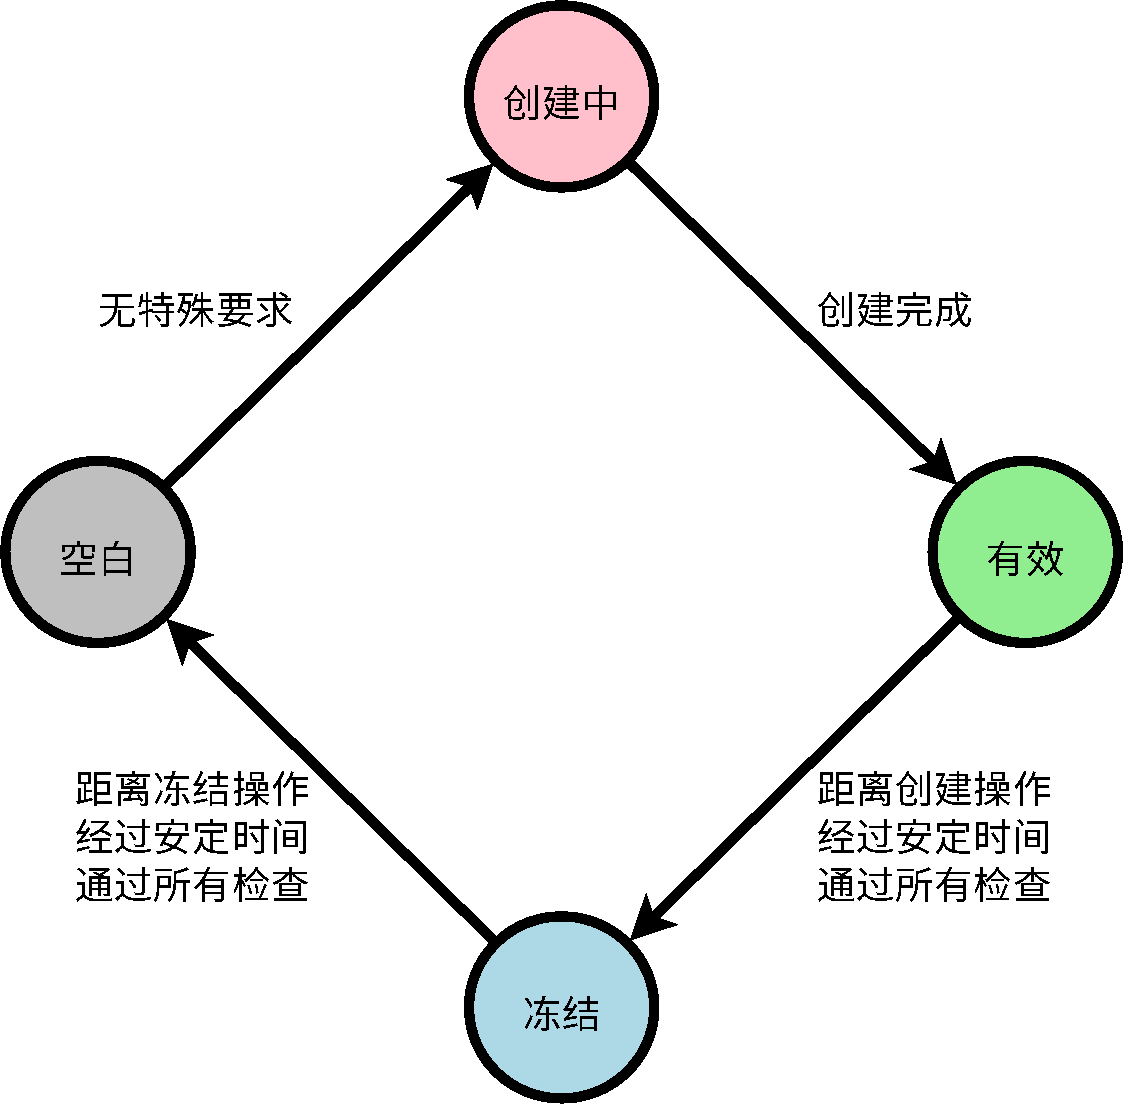
\includegraphics[width=0.72\textwidth]{Figure/image5.pdf}
    \caption{权能的生命周期}
    \label{fig:2-1-capability-lifecycle}
\end{figure}

安定时间要求至少是内核最坏执行时间两倍的原因如下：在调用权能冻结操作时，我们会先更新权能的时间戳，然后再通过原子操作标记该权能为被冻结。因此我们有如下的时间轴：

\begin{figure}[htbp]
    \centering
    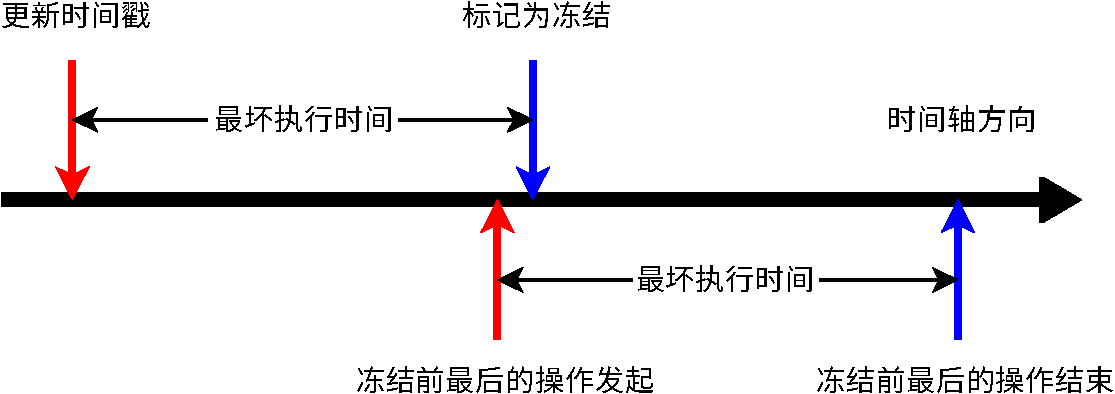
\includegraphics[width=0.72\textwidth]{Figure/image6.pdf}
    \caption{权能冻结的时间线}
    \label{fig:2-2-capability-freeze-timeline}
\end{figure}

从该时间轴中可以看出，从更新时间戳到冻结前的最后操作结束最多可能经过两个内核最坏执行时间。在实际使用中，推荐将安定时间至少配置为内核最坏执行时间的20倍\footnote{推荐高出一个数量级}，因为在工程中对最坏执行时间的估算往往只有数量级是准确的。

上面所说明的原理对于权能的创建------冻结安定时间也是一样的，在此不赘述。

\subsection{权能表结构}\label{subsec:2-capability-table-structure}

权能表可以被组织成多级结构。组织的具体方法是，在权能表内部放入权能表权能，这样权能表就可以组织成一个基数树。在对内核对象做操作时，需要传递一个权能号，指定这个权能在当前进程的权能表内部的位置。权能号最多可以编码两级查找。我们把一级查找可以达到的范围称为主权能表，把只有二级查找才能到达的范围称为扩展权能表。在32位系统下，权能号是一个16位的值；在64位系统下，权能号是一个32位的值。在更高位的系统下，依此类推。具体的编码方法如下：

\begin{xltabular}{\textwidth}{@{}>{\hsize=0.6388\hsize\raggedright\arraybackslash}X>{\hsize=0.7677\hsize\raggedright\arraybackslash}X>{\hsize=1.5935\hsize\raggedright\arraybackslash}X@{}}
\caption{权能号的编码方法}\label{tab:2-2-capability-number-encoding}\\
\toprule
系统位数 & 编码类型 & 编码方法\tabularnewline
\endfirsthead
\toprule
系统位数 & 编码类型 & 编码方法\tabularnewline
\midrule
\endhead
\bottomrule
\endlastfoot
\multirow{2}{*}{32位系统} & 一级查找编码 & {[}15:8{]}保留 {[}7{]}固定为0
{[}6:0{]}位置\tabularnewline
& 二级查找编码 & {[}15{]}保留 {[}14:8{]}子表位置 {[}7{]}固定为1
{[}6:0{]}在子表中的位置\tabularnewline
\multirow{2}{*}{64位系统} & 一级查找编码 & {[}32:16{]}保留 {[}15{]}固定为0
{[}14:0{]}位置\tabularnewline
& 二级查找编码 & {[}32{]}保留 {[}31:16{]}子表位置 {[}15{]}固定为1
{[}14:0{]}在子表中的位置\tabularnewline
\end{xltabular}

可以看出，在32位系统下，单个权能表中最多可以有2\textsuperscript{7}=128个权能，在64位系统下这一个值则为2\textsuperscript{15}=32768。在 RME 中这个值由宏 RME\_CID\_2L 代表。与 seL4 等系统不同，RME 的权能表不支持基于基数树的无限级别查找。也即，扩展权能表内的权能表权能指向的权能表\footnote{也即二级扩展权能表}中的权能，不被认为在扩展权能表之内，无法通过二级查找编码被直接使用\footnote{也即``我的附庸的附庸，不是我的附庸''}。如果要使用的话，必须通过权能传递调用传递到扩展权能表之内，才可以通过二级查找编码被调用。

如下图所示，在主权能表中有一个指向扩展权能表的权能表权能，它被放置在权能号4的位置上。该扩展权能表中的权能也可以通过二级查找编码访问。在该扩展权能表的权能号2的位置上有一个指向二级扩展权能表的权能表权能，该权能本身可以使用值为4:2的二级查找编码被访问，但它指向的二级扩展权能表中的权能则无法通过二级查找编码直接访问了。图中不能从主权能表被访问的部分以灰色表示。

\begin{figure}[htbp]
    \centering
    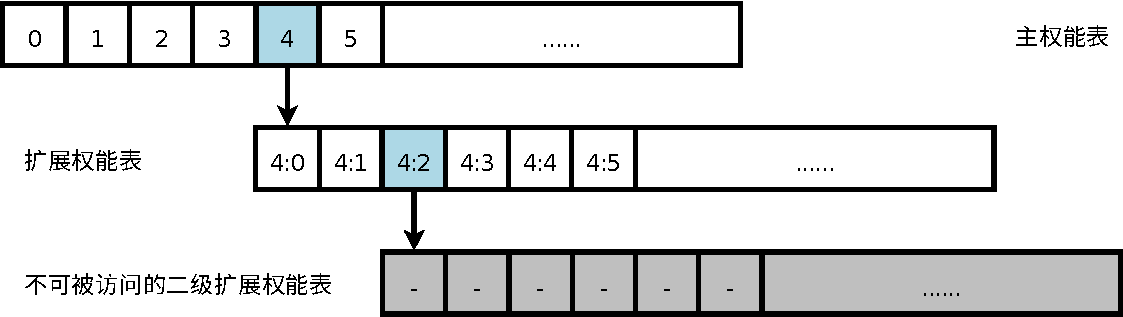
\includegraphics[width=0.72\textwidth]{Figure/image7.pdf}
    \caption{权能表结构图}
    \label{fig:2-3-capability-table-structure}
\end{figure}

\section{权能表功能列表}\label{sec:2-capability-table-function-list}

与权能表有关的内核功能如下：

\begin{xltabular}{\textwidth}{@{}>{\hsize=1.1605\hsize\raggedright\arraybackslash}X>{\hsize=0.8843\hsize\raggedright\arraybackslash}X>{\hsize=0.9552\hsize\raggedright\arraybackslash}X@{}}
\caption{权能表相关内核功能}\label{tab:2-3-capability-table-kernel-functions}\\
\toprule
调用号 & 类型 & 用途\tabularnewline
\endfirsthead
\toprule
调用号 & 类型 & 用途\tabularnewline
\midrule
\endhead
\bottomrule
\endlastfoot
RME\_SVC\_CPT\_CRT & 系统调用 & 创建权能表\tabularnewline
RME\_SVC\_CPT\_DEL & 系统调用 & 删除权能表\tabularnewline
RME\_SVC\_CPT\_ADD & 系统调用 & 权能传递\tabularnewline
RME\_SVC\_CPT\_FRZ & 系统调用 & 权能冻结\tabularnewline
RME\_SVC\_CPT\_REM & 系统调用 & 权能移除\tabularnewline
\end{xltabular}

权能表权能的操作标志如下：

\begin{xltabular}{\textwidth}{@{}>{\hsize=0.9567\hsize\raggedright\arraybackslash}X>{\hsize=0.6339\hsize\raggedright\arraybackslash}X>{\hsize=1.4095\hsize\raggedright\arraybackslash}X@{}}
\caption{权能表操作标志}\label{tab:2-4-capability-table-operation-flags}\\
\toprule
标志 & 位 & 用途\tabularnewline
\endfirsthead
\toprule
标志 & 位 & 用途\tabularnewline
\midrule
\endhead
\bottomrule
\endlastfoot
RME\_CPT\_FLAG\_CRT & {[}0{]} &
允许在该权能表中创建权能。\tabularnewline
RME\_CPT\_FLAG\_DEL & {[}1{]} &
允许删除该权能表中的权能。\tabularnewline
RME\_CPT\_FLAG\_FRZ & {[}2{]} &
允许冻结该权能表中的权能。\tabularnewline
RME\_CPT\_FLAG\_ADD\_SRC & {[}3{]} &
允许该权能表在权能传递作为来源表。\tabularnewline
RME\_CPT\_FLAG\_ADD\_DST & {[}4{]} &
允许该权能表在权能传递作为目标表。\tabularnewline
RME\_CPT\_FLAG\_REM & {[}5{]} &
允许移除该权能表中的权能。\tabularnewline
RME\_CPT\_FLAG\_PRC\_CRT & {[}6{]} &
允许在创建进程时将该权能表作为进程的权能表。\tabularnewline
RME\_CPT\_FLAG\_PRC\_CPT & {[}7{]} &
允许用该权能表替换某进程的权能表。\tabularnewline
\end{xltabular}

关于上表中的位{[}6{]}和位{[}7{]}，请参见\ref{subsec:4-create-a-process}
和\ref{subsec:4-change-process-capability-table}
。

\subsection{创建权能表}\label{subsec:2-create-a-capability-table}

该操作会创建一个权能表，并将其权能放入某个已存在的权能表。在权能表是一种内核对象，因此创建时需要指定其所使用的内核内存。在 RME 中，我们采用内核内存权能和内核起始相对虚拟地址的方法确定该内核对象的真实内核虚拟地址。每一个内核内存权能都会指定一个允许范围\footnote{由内核内存起始绝对虚拟地址和内核内存终止绝对虚拟地址组成}，只有这个范围内的内核内存才能在创建内核对象时使用。这个内核内存权能的内核起始绝对虚拟地址加上在创建内核对象时额外指定的内核起始相对虚拟地址（Relative
Address,
Raddr）才是内核对象的真实内核虚拟地址。这一点对于包括权能表在内的其他的内核对象都是相同的，在后面的章节中将不再赘述。关于内核内存权能的详细信息请参见\ref{sec:3-kernel-memory-function-list}
。

创建权能表操作需要如下几个参数：

\begin{xltabular}{\textwidth}{@{}>{\hsize=0.7639\hsize\raggedright\arraybackslash}X>{\hsize=0.6758\hsize\raggedright\arraybackslash}X>{\hsize=0.6758\hsize\raggedright\arraybackslash}X>{\hsize=1.8846\hsize\raggedright\arraybackslash}X@{}}
\caption{创建权能表的所需参数}\label{tab:2-5-create-capability-table-parameters}\\
\toprule
参数名称 & 类型 & 域 & 描述\tabularnewline
\endfirsthead
\toprule
参数名称 & 类型 & 域 & 描述\tabularnewline
\midrule
\endhead
\bottomrule
\endlastfoot
Svc\_Num & ptr\_t & N & 必须为 RME\_SVC\_CPT\_CRT。\tabularnewline
Cap\_Cpt\_Crt & cid\_t & C &
一个对应于必须拥有 RME\_CPT\_FLAG\_CRT 属性的权能表权能的权能号，该权能号对应的权能指向要接受此新创建的权能表权能的权能表。该权能号可以是一级或二级查找编码。\tabularnewline
Cap\_Kom & cid\_t & P1.D1 &
一个内核内存权能号，其标识的内核内存范围必须能够放下整个权能表，并且要拥有 RME\_KOM\_FLAG\_CPT 属性。该权能号可以是一级或二级查找编码。\tabularnewline
Cap\_Crt & cid\_t & P1.D0 &
一个对应于接受该新创建的权能表权能的权能表的某位置的权能号。该权能号对应的权能必须是空白的。该权能号只能是一级查找编码。\tabularnewline
Raddr & ptr\_t & P2 &
新创建的权能表要使用的内核起始相对虚拟地址。这个地址是相对于 Cap\_Kom 对应的内核权能的起始虚拟地址的。\tabularnewline
Entry\_Num & ptr\_t & P3 &
该权能表包含的表项数目，必须在 1 到 RME\_CID\_2L 之间。如果 RME\_CPT\_ENTRY\_MAX\footnote{见 7.3.2} 被定义为一个小于 RME\_CID\_2L 且不为 0 的值，则该数目必须在 1 到 RME\_CPT\_ENTRY\_MAX 之间。\tabularnewline
\end{xltabular}

该操作的返回值可能如下：

\begin{xltabular}{\textwidth}{@{}>{\hsize=0.7950\hsize\raggedright\arraybackslash}X>{\hsize=1.2050\hsize\raggedright\arraybackslash}X@{}}
\caption{创建权能表的可能返回值}\label{tab:2-6-create-capability-table-return-values}\\
\toprule
返回值 & 意义\tabularnewline
\endfirsthead
\toprule
返回值 & 意义\tabularnewline
\midrule
\endhead
\bottomrule
\endlastfoot
    0 & 操作成功。\tabularnewline
    RME\_ERR\_CPT\_RANGE & 传入的权能表权能数目参数超出了允许的范围。\tabularnewline
    RME\_ERR\_CPT\_RANGE & Cap\_Cpt\_Crt 的一级/二级查找超出了范围。\tabularnewline
    RME\_ERR\_CPT\_RANGE & Cap\_Kom 的一级/二级查找超出了范围。\tabularnewline
    RME\_ERR\_CPT\_RANGE & Cap\_Crt 的一级查找超出了范围。\tabularnewline
    RME\_ERR\_CPT\_FROZEN & Cap\_Cpt\_Crt 的一级/二级查找的权能已经被冻结。\tabularnewline
    RME\_ERR\_CPT\_FROZEN & Cap\_Kom 的一级/二级查找的权能已经被冻结。\tabularnewline
    RME\_ERR\_CPT\_FROZEN & Cap\_Crt 被冻结，或者其它核正在该处创建权能。\tabularnewline
    RME\_ERR\_CPT\_TYPE & Cap\_Cpt\_Crt 不是权能表权能。\tabularnewline
    RME\_ERR\_CPT\_TYPE & Cap\_Kom 不是内核内存权能。\tabularnewline
    RME\_ERR\_CPT\_FLAG & Cap\_Cpt\_Crt 无 RME\_CPT\_FLAG\_CRT 属性。\tabularnewline
    RME\_ERR\_CPT\_FLAG & Cap\_Kom 无 RME\_KOM\_FLAG\_CPT 属性，或范围错误。\tabularnewline
    RME\_ERR\_CPT\_EXIST & Cap\_Crt 不是空白权能。\tabularnewline
    RME\_ERR\_CPT\_KOT & 分配内核内存失败。\tabularnewline
\end{xltabular}

\subsection{删除权能表}\label{subsec:2-delete-a-capability-table}

该操作会删除一个权能表。被删除的权能表必须不含有权能，也即其全部权能位置应该都是空白的。删除权能表需要以下几个参数：

\begin{xltabular}{\textwidth}{@{}>{\hsize=0.7639\hsize\raggedright\arraybackslash}X>{\hsize=0.6758\hsize\raggedright\arraybackslash}X>{\hsize=0.6758\hsize\raggedright\arraybackslash}X>{\hsize=1.8846\hsize\raggedright\arraybackslash}X@{}}
\caption{删除权能表的所需参数}\label{tab:2-7-delete-capability-table-parameters}\\
\toprule
参数名称 & 类型 & 域 & 描述\tabularnewline
\endfirsthead
\toprule
参数名称 & 类型 & 域 & 描述\tabularnewline
\midrule
\endhead
\bottomrule
\endlastfoot
Svc\_Num & ptr\_t & N & 必须为 RME\_SVC\_CPT\_DEL。\tabularnewline
Cap\_Cpt\_Del & cid\_t & C &
一个对应于必须拥有 RME\_CPT\_FLAG\_DEL 属性的权能表权能的权能号，该权能号对应的权能指向含有正被删除的权能表权能的权能表。该权能号可以是一级或者二级查找编码。\tabularnewline
Cap\_Del & cid\_t & P1 &
一个对应于将被删除的权能表权能的权能号。该权能号对应的权能必须是一个权能表权能。该权能号只能是一级查找编码。\tabularnewline
\end{xltabular}

该操作的返回值可能如下：

\begin{xltabular}{\textwidth}{@{}>{\hsize=0.7450\hsize\raggedright\arraybackslash}X>{\hsize=1.2550\hsize\raggedright\arraybackslash}X@{}}
\caption{删除权能表的可能返回值}\label{tab:2-8-delete-capability-table-return-values}\\
\toprule
返回值 & 意义\tabularnewline
\endfirsthead
\toprule
返回值 & 意义\tabularnewline
\midrule
\endhead
\bottomrule
\endlastfoot
    0 & 操作成功。\tabularnewline
    RME\_ERR\_CPT\_RANGE & Cap\_Cpt\_Del 的一级/二级查找超出了范围。\tabularnewline
    RME\_ERR\_CPT\_RANGE & Cap\_Del 的一级查找超出了范围。\tabularnewline
    RME\_ERR\_CPT\_FROZEN & Cap\_Cpt\_Del 的一级/二级查找的权能已经被冻结。\tabularnewline
    RME\_ERR\_CPT\_FROZEN & Cap\_Del 未被冻结。\tabularnewline
    RME\_ERR\_CPT\_TYPE & Cap\_Cpt\_Del 不是权能表权能。\tabularnewline
    RME\_ERR\_CPT\_TYPE & Cap\_Del 不是权能表权能。\tabularnewline
    RME\_ERR\_CPT\_NULL & Cap\_Del 为空白权能。\tabularnewline
    RME\_ERR\_CPT\_NULL & 两个核同时试图删除该权能表，此时未成功的核返回该值。\tabularnewline
    RME\_ERR\_CPT\_FLAG & Cap\_Cpt\_Del 无 RME\_CPT\_FLAG\_DEL 属性。\tabularnewline
    RME\_ERR\_CPT\_QUIE & Cap\_Del 不安定。\tabularnewline
    RME\_ERR\_CPT\_EXIST & Cap\_Del 对应的权能表内还有权能。\tabularnewline
    RME\_ERR\_CPT\_REFCNT & Cap\_Del 的引用计数不为 0，或者不为根权能。\tabularnewline
\end{xltabular}

\subsection{权能传递}\label{subsec:2-transfer-a-capability}

该操作会将一个权能表中的某个权能传递到另外一个权能表的空白位置中。新创建的目标权能的父权能是源权能，并且源权能的引用计数会增加1。在权能表之间进行权能传递需要以下几个参数：

\begin{xltabular}{\textwidth}{@{}>{\hsize=0.7639\hsize\raggedright\arraybackslash}X>{\hsize=0.6758\hsize\raggedright\arraybackslash}X>{\hsize=0.6758\hsize\raggedright\arraybackslash}X>{\hsize=1.8846\hsize\raggedright\arraybackslash}X@{}}
\caption{权能传递的所需参数}\label{tab:2-9-capability-transfer-parameters}\\
\toprule
参数名称 & 类型 & 域 & 描述\tabularnewline
\endfirsthead
\toprule
参数名称 & 类型 & 域 & 描述\tabularnewline
\midrule
\endhead
\bottomrule
\endlastfoot
Svc\_Num & ptr\_t & N & 必须为 RME\_SVC\_CPT\_ADD。\tabularnewline
Cap\_Cpt\_Dst & cid\_t & P1.D1 &
一个对应于必须拥有 RME\_CPT\_FLAG\_ADD\_DST 属性的权能表权能的权能号，该权能号对应的权能指向目标权能表。该权能号可以是一级或者二级查找编码。\tabularnewline
Cap\_Dst & cid\_t & P1.D0 &
一个对应于将接受被传递的权能的权能号。该权能号对应的权能必须是空白的。该权能号只能是一级查找编码。\tabularnewline
Cap\_Cpt\_Src & cid\_t & P2.D1 &
一个对应于必须拥有 RME\_CPT\_FLAG\_ADD\_SRC 属性的权能表权能的权能号，该权能号对应的权能指向源权能表。该权能号可以是一级或者二级查找编码。\tabularnewline
Cap\_Src & cid\_t & P2.D0 &
一个对应于将传递的权能的权能号。该权能号对应的权能必须不为空白而且没有冻结。该权能号只能是一级查找编码。\tabularnewline
Flags & ptr\_t & P3 &
要传递的操作标志属性。只有这个操作标志允许的操作才能被新创建的权能执行。\tabularnewline
\end{xltabular}

需要注意的是，对于内核内存权能，其传递时还需要置于系统调用号 N 和权能表权能号 C 中的额外位来辅助确定其操作标志属性。具体的参数传递方法请参见\ref{sec:3-kernel-memory-function-list}
。

该操作的返回值可能如下：

\begin{xltabular}{\textwidth}{@{}>{\hsize=0.6791\hsize\raggedright\arraybackslash}X>{\hsize=1.3209\hsize\raggedright\arraybackslash}X@{}}
\caption{权能传递的可能返回值}\label{tab:2-10-capability-transfer-return-values}\\
\toprule
返回值 & 意义\tabularnewline
\endfirsthead
\toprule
返回值 & 意义\tabularnewline
\midrule
\endhead
\bottomrule
\endlastfoot
    0 & 操作成功。\tabularnewline
    RME\_ERR\_CPT\_RANGE & Cap\_Cpt\_Dst 或 Cap\_Cpt\_Src 的一级/二级查找超出了范围。\tabularnewline
    RME\_ERR\_CPT\_RANGE & Cap\_Dst 或 Cap\_Src 的一级查找超出了范围。\tabularnewline
    RME\_ERR\_CPT\_FROZEN & Cap\_Cpt\_Dst 或 Cap\_Cpt\_Src 的一级/二级查找的权能被冻结。\tabularnewline
    RME\_ERR\_CPT\_FROZEN & Cap\_Src 被冻结。\tabularnewline
    RME\_ERR\_CPT\_TYPE & Cap\_Cpt\_Dst 或 Cap\_Cpt\_Src 不是权能表权能。\tabularnewline
    RME\_ERR\_CPT\_NULL & Cap\_Src 为空白权能。\tabularnewline
    RME\_ERR\_CPT\_FLAG & Cap\_Cpt\_Src 无 RME\_CPT\_FLAG\_ADD\_SRC 属性。\tabularnewline
    RME\_ERR\_CPT\_FLAG & Cap\_Cpt\_Dst 无 RME\_CPT\_FLAG\_ADD\_DST 属性。\tabularnewline
    RME\_ERR\_CPT\_FLAG & Cap\_Src 的操作标志属性与传入的操作标志属性冲突，也即传入的属性包括了 Cap\_Src 不允许的操作或者操作范围。\tabularnewline
    RME\_ERR\_CPT\_FLAG & 传入的操作标志属性是不合法的，比如操作范围上下限冲突，或者不允许在传递产生的权能上做任何操作。\tabularnewline
    RME\_ERR\_CPT\_EXIST & Cap\_Dst 不是空白权能。\tabularnewline
    RME\_ERR\_CPT\_REFCNT & Cap\_Src 的引用计数超过了系统允许的最大范围。在 32 位系统中上限是 $2^{23}-1$，在 64 位系统中上限是 $2^{46}-1$。通常这是足够的。\tabularnewline
\end{xltabular}

\needspace{30\baselineskip}
\subsection{权能冻结}\label{subsec:2-freeze-a-capability}
\nopagebreak[4]

该操作会将一个权能表中的某个权能冻结。如果一个权能被冻结，那么在安定时间之后，能够保证从这个权能发起的，对这个权能指向的内核对象的操作在内核中全部停止，此时可以删除或移除该权能。注意，这并不等价于该权能指向的内核对象的全部操作都停止，因为还可能有其他权能指向这个内核对象，而从这些权能发起的内核对象操作仍然可以进行。如果根权能被冻结，那么才能保证该内核对象上的所有操作都停止，此时才可以删除该权能和内核对象。冻结权能操作也是由比较交换操作原子执行的；但它失败时我们知道一定有其他核成功帮助我们冻结了该权能，因此仍然返回成功。

\needspace{20\baselineskip}
冻结一个权能需要如下参数：

\begin{xltabular}{\textwidth}{@{}>{\hsize=0.7639\hsize\raggedright\arraybackslash}X>{\hsize=0.6758\hsize\raggedright\arraybackslash}X>{\hsize=0.6758\hsize\raggedright\arraybackslash}X>{\hsize=1.8846\hsize\raggedright\arraybackslash}X@{}}
\caption{权能冻结的所需参数}\label{tab:2-11-capability-freeze-parameters}\\
\toprule
参数名称 & 类型 & 域 & 描述\tabularnewline
\endfirsthead
\toprule
参数名称 & 类型 & 域 & 描述\tabularnewline
\midrule
\endhead
\bottomrule
\endlastfoot
Svc\_Num & ptr\_t & N & 必须为 RME\_SVC\_CPT\_FRZ。\tabularnewline
Cap\_Cpt\_Frz & cid\_t & C &
一个对应于必须拥有 RME\_CPT\_FLAG\_FRZ 属性的权能表权能的权能号，该权能号对应的权能指向含有正被冻结的权能的权能表。该权能号可以是一级或者二级查找编码。\tabularnewline
Cap\_Frz & cid\_t & P1 &
一个对应于将被冻结的权能的权能号。该权能号只能是一级查找编码。\tabularnewline
\end{xltabular}

该操作的返回值可能如下：

\begin{xltabular}{\textwidth}{@{}>{\hsize=0.7950\hsize\raggedright\arraybackslash}X>{\hsize=1.2050\hsize\raggedright\arraybackslash}X@{}}
\caption{权能冻结的可能返回值}\label{tab:2-12-capability-freeze-return-values}\\
\toprule
返回值 & 意义\tabularnewline
\endfirsthead
\toprule
返回值 & 意义\tabularnewline
\midrule
\endhead
\bottomrule
\endlastfoot
    0 & 操作成功。\tabularnewline
    RME\_ERR\_CPT\_RANGE & Cap\_Cpt\_Frz 的一级/二级查找超出了范围。\tabularnewline
    RME\_ERR\_CPT\_RANGE & Cap\_Frz 的一级查找超出了范围。\tabularnewline
    RME\_ERR\_CPT\_FROZEN & Cap\_Cpt\_Frz 的一级/二级查找的权能已经被冻结。\tabularnewline
    RME\_ERR\_CPT\_FROZEN & Cap\_Frz 已经被冻结，无需再次冻结，或者正在被创建。\tabularnewline
    RME\_ERR\_CPT\_TYPE & Cap\_Cpt\_Frz 不是权能表权能。\tabularnewline
    RME\_ERR\_CPT\_NULL & Cap\_Frz 为空白权能。\tabularnewline
    RME\_ERR\_CPT\_FLAG & Cap\_Cpt\_Frz 无 RME\_CPT\_FLAG\_FRZ 属性。\tabularnewline
    RME\_ERR\_CPT\_QUIE & Cap\_Frz 不安定。\tabularnewline
    RME\_ERR\_CPT\_REFCNT & Cap\_Frz 的引用计数不为 0。\tabularnewline
\end{xltabular}

\subsection{权能移除}\label{subsec:2-remove-a-capability}

该操作会将一个权能表中的某个权能移除。被移除的权能必须不是根权能\footnote{对根权能应当使用删除操作}。移除一个权能不会导致与之相关联的内核对象被移除，被移除的仅仅是权能本身\footnote{删除操作则只能对不被引用的根权能使用，并且会同时删除根权能和内核对象}。移除权能操作也是由比较交换操作原子执行的；但它失败时我们知道一定有其他核成功帮助我们移除了该权能，因此仍然返回成功。

移除一个权能需要如下参数：

\begin{xltabular}{\textwidth}{@{}>{\hsize=0.7639\hsize\raggedright\arraybackslash}X>{\hsize=0.6758\hsize\raggedright\arraybackslash}X>{\hsize=0.6758\hsize\raggedright\arraybackslash}X>{\hsize=1.8846\hsize\raggedright\arraybackslash}X@{}}
\caption{权能移除的所需参数}\label{tab:2-13-capability-removal-parameters}\\
\toprule
参数名称 & 类型 & 域 & 描述\tabularnewline
\endfirsthead
\toprule
参数名称 & 类型 & 域 & 描述\tabularnewline
\midrule
\endhead
\bottomrule
\endlastfoot
Svc\_Num & ptr\_t & N & 必须为 RME\_SVC\_CPT\_REM。\tabularnewline
Cap\_Cpt\_Rem & cid\_t & C &
一个对应于必须拥有 RME\_CPT\_FLAG\_REM 属性的权能表权能的权能号，该权能号对应的权能指向含有正被移除的权能的权能表。该权能号可以是一级或者二级查找编码。\tabularnewline
Cap\_Rem & cid\_t & P1 &
一个对应于将被移除的权能的权能号。该权能号只能是一级查找编码。\tabularnewline
\end{xltabular}

该操作的返回值可能如下：

\begin{xltabular}{\textwidth}{@{}>{\hsize=0.7554\hsize\raggedright\arraybackslash}X>{\hsize=1.2446\hsize\raggedright\arraybackslash}X@{}}
\caption{权能移除的可能返回值}\label{tab:2-14-capability-removal-return-values}\\
\toprule
返回值 & 意义\tabularnewline
\endfirsthead
\toprule
返回值 & 意义\tabularnewline
\midrule
\endhead
\bottomrule
\endlastfoot
    0 & 操作成功。\tabularnewline
    RME\_ERR\_CPT\_RANGE & Cap\_Cpt\_Rem 的一级/二级查找超出了范围。\tabularnewline
    RME\_ERR\_CPT\_RANGE & Cap\_Rem 的一级查找超出了范围。\tabularnewline
    RME\_ERR\_CPT\_FROZEN & Cap\_Cpt\_Rem 的一级/二级查找的权能已经被冻结。\tabularnewline
    RME\_ERR\_CPT\_FROZEN & Cap\_Rem 未被冻结。\tabularnewline
    RME\_ERR\_CPT\_TYPE & Cap\_Cpt\_Rem 不是权能表权能。\tabularnewline
    RME\_ERR\_CPT\_NULL & Cap\_Rem 为空白权能。\tabularnewline
    RME\_ERR\_CPT\_NULL & 两个核同时试图移除该权能，此时未成功的核返回该值。\tabularnewline
    RME\_ERR\_CPT\_FLAG & Cap\_Cpt\_Rem 无 RME\_CPT\_FLAG\_REM 属性。\tabularnewline
    RME\_ERR\_CPT\_QUIE & Cap\_Rem 不安定。\tabularnewline
    RME\_ERR\_CPT\_ROOT & Cap\_Rem 为根权能，不能使用移除，请使用删除操作。\tabularnewline
\end{xltabular}

\section{本章参考文献}\label{sec:2-chapter-bibliography}

\protect\phantomsection\label{cite:2-1}

\noindent {[}1{]} J. B. Dennis and E. C. Van Horn, ``Programming semantics for multiprogrammed computations,'' \textit{Communications of the ACM}, vol. 9, pp. 143--155, 1966.

\protect\phantomsection\label{cite:2-2}

\noindent {[}2{]} J. S. Shapiro, J. M. Smith, and D. J. Farber, \textit{EROS: A Fast Capability System}, vol. 33. ACM, 1999.

\protect\phantomsection\label{cite:2-3}

\noindent {[}3{]} R. J. Feiertag and P. G. Neumann, ``The foundations of a provably secure operating system (PSOS),'' in \textit{Proceedings of the National Computer Conference}, 1979, pp. 329--334.

\protect\phantomsection\label{cite:2-4}

\noindent {[}4{]} Q. Wang, Y. Ren, M. Scaperoth, and G. Parmer, ``Speck: a kernel for scalable predictability,'' in \textit{Proceedings of the IEEE Real-Time and Embedded Technology and Applications Symposium (RTAS)}, 2015, pp. 121--132.

\protect\phantomsection\label{cite:2-5}

\noindent {[}5{]} G. Klein, K. Elphinstone, G. Heiser, J. Andronick, D. Cock, P. Derrin, et al., ``seL4: formal verification of an OS kernel,'' in \textit{Proceedings of the ACM SIGOPS 22nd Symposium on Operating Systems Principles}, Big Sky, MT, USA, 2009.

\protect\phantomsection\label{cite:2-6}

\noindent {[}6{]} B. W. Lampson, ``Protection,'' \textit{ACM SIGOPS Operating Systems Review}, vol. 8, pp. 18--24, 1974.


\chapter{页表和内存管理}\label{ch:page-tables-and-memory-management}

\section{内存管理概述}\label{sec:3-memory-management-overview}

内存管理（Memory Management）指的是对物理内存（Physical
Memory）及虚拟地址空间（Virtual Address
Space，VAS）进行的分配和回收操作。要保证内存管理的安全性，硬件上的支持是必要的。RME 操作系统的内存管理支持内存保护单元（Memory
Protection Unit，MPU）环境和内存管理单元（Memory Management
Unit，MMU）环境，并且它们被抽象成了相同的页表数据结构。本章中所用到的术语的定义如下：

\begin{xltabular}{\textwidth}{@{}>{\hsize=0.7749\hsize\raggedright\arraybackslash}X>{\hsize=1.2251\hsize\raggedright\arraybackslash}X@{}}
\caption{页目录术语定义}\label{tab:3-1-page-directory-terminology}\\
\toprule
术语 & 定义\tabularnewline
\endfirsthead
\toprule
术语 & 定义\tabularnewline
\midrule
\endhead
\bottomrule
\endlastfoot
页表（Page Table，PT） &
指的是整个页表本身，包括了顶层页目录和中间的各个级别的页目录，是一棵地址树的总称。\tabularnewline
页目录（Page Directory，PD） &
指的是页表中的一级，其中最顶层的一级被称为顶层页目录。\tabularnewline
页表项（Page Entry，PE） &
指的是页目录表格中的一项，它可能指向一个页，也可能指向下一级页目录。其中，我们把指向页的叫做末端页表项（Page
Terminal Entry，PTE），把指向下一级页目录的叫做中间页表项（Page
Intermediate Entry，PIE）。\tabularnewline
\end{xltabular}

\section{页表的操作和结构}\label{sec:3-page-table-operations-and-structure}

页表是由一系列页目录组成的多层基数树（Radix Trie/Radix
Tree）结构。页目录的每一个槽位都被固定为一个机器字的长度。页目录中的每一个槽位都可以放置以下三种数据之一：下级页目录物理地址、页表项物理地址及属性或空页表项。如果存放的是下级页目录物理地址，那么代表此处有一个下级页目录，该部分虚拟地址的映射关系要查询该页目录决定；如果存放的是页表项物理地址及属性，则代表此虚拟地址处有一个页表项被映射，并且可以得知该页的访问属性；如果存放的是空页表项，那么则说明这个虚拟地址处没有任何东西被映射。在 RME 中，页表是需要用户手动构造的，这和 Composite 等一系列微内核的解决方法是一致的\hyperref[cite:3-1]{{[}1{]}}。

\subsection{内核内存和用户内存}\label{subsec:3-kernel-memory-and-user-memory}

RME 的系统内存被分为两部分：一部分是内核内存，一部分是用户内存。和 Composite、L4 等微内核不同，在 RME 系统中，内核内存映射是在一开始就完全建立\footnote{静态或半静态分配}的，并且不可修改。这使得 RME 完全不需要内存动态类型机制\footnote{这种机制被Composite、seL4等系统采用\hyperref[cite:3-1]{{[}1{]}}\hyperref[cite:3-3]{{[}3{]}}。在 RME 中它其实也可以被受信任的用户态服务器实现}，而且内存管理系统完全可并行化，同时彻底免去了内核内存内容泄露的可能。对于MMU环境，在创建顶层页目录时，系统会将在启动时就创建好的内核页目录映射到顶层页目录之内；对于MPU环境，由于内核态通常都有对整个内存的访问权限，因此在所有页目录中我们只需要用户页就可以了\footnote{某些架构（如 Tricore 等）需要保留一个或者多个MPU寄存器组给内核态，但是这些页并不会反映在页表中}。

在系统启动时，所有的用户物理内存页都被加入了启动进程（Init）的页表之中。在这种添加结束之后，通常而言不再允许系统凭空地创造物理内存页框，除非使用自定义内核调用\footnote{见第~\ref{sec:8-kernel-call-implementation-overview}~节}。在创建新进程时，新进程的页表的页表项是必须从其他进程处添加过来的。在添加时，可以指定这个页的访问属性，并且所指定的访问属性一定要是父页面的访问属性的一个子集。RME 系统中，页访问的标准属性如下表：

\begin{xltabular}{\textwidth}{@{}>{\hsize=0.5857\hsize\raggedright\arraybackslash}X>{\hsize=0.7809\hsize\raggedright\arraybackslash}X>{\hsize=1.6334\hsize\raggedright\arraybackslash}X@{}}
\caption{页访问的标准属性}\label{tab:3-2-standard-page-access-attributes}\\
\toprule
名称 & 标识符 & 意义\tabularnewline
\endfirsthead
\toprule
名称 & 标识符 & 意义\tabularnewline
\midrule
\endhead
\bottomrule
\endlastfoot
可读 & RME\_PGT\_READ & 这个页面是可读取的。\tabularnewline
可写 & RME\_PGT\_WRITE & 这个页面是可写入的。\tabularnewline
可执行 & RME\_PGT\_EXECUTE &
这个页面的是可作为代码执行的。\tabularnewline
可缓存 & RME\_PGT\_CACHE & 这个页面的内容可以被缓存。\tabularnewline
可缓冲 & RME\_PGT\_BUFFER & 这个页面的写入可以被缓冲。\tabularnewline
静态 & RME\_PGT\_STATIC &
这个页面是总被映射的静态页。这意味着，MPU环境下或在手动更新TLB的MMU环境下，这个页总是被映射，而非等到缺页中断来临时映射。\tabularnewline
\end{xltabular}

值得注意的是，在某些架构中，上面的某些位可能不会全部都具有意义。比如，对于绝大多数自动更新快表（Trans
Look-aside
Buffer，TLB）的MMU环境，静态属性是没有意义的；对于某些架构，读和写是一起实现的，因此不具有分立的读写控制。

为了实现用户态对在创建内核对象时对内核内存的管理，系统中的内核对象使用一个内核对象登记表进行管理。内核对象登记表是一个位图，里面存储了内核对象对于虚拟地址的占用。这个位图保证了在同一段内核虚拟地址上，不可能同时存在两个内核对象。

为了防止某些有权创建内核对象的系统组件在出错或被入侵时大量创建内核对象从而耗尽内核内存，发动拒绝服务（Denial
of
Service，DoS）攻击，因此引入了内核内存权能来管理内核内存。内核内存权能的概念参考了 Fiasco.OC 的内核对象工厂（Factory）\hyperref[cite:3-4]{{[}4{]}}。在创建任何一个内核对象时，都需要内核内存权能；该内核内存权能标志了允许用来创建内核对象的内核虚拟内存地址范围，以及允许在这段内存上创建哪些对象。只有当被创建的内核对象完全落在这个范围之内，并且该内核内存权能的标志位允许创建该种对象时，创建操作才能够被继续进行，否则将返回一个错误，从而限制某些被感染的恶意内核组件发起拒绝服务攻击。

\subsection{页目录的属性}\label{subsec:3-page-directory-attributes}

在 RME 操作系统中，页目录有四个属性。这四个属性唯一决定了页目录的状态。我们下面将分别介绍这四种属性。

\subsubsection{映射起始地址}\label{subsubsec:3-mapping-base-address}

映射起始地址指该层页目录开始映射的虚拟地址。这个页目录的第一个槽位的物理内存或者映射的二级页表的起始地址，就是这个虚拟地址。当我们试图把一个更底层的页目录映射到某高层次页目录的某位置时，我们可能需要检查底层的虚拟地址是否和高层的虚拟地址匹配，从而决定能否进行该映射。当然，这个检查仅仅在使用MPU的系统中是必须的。在使用MMU的系统中，由于一个页目录经常会被映射进不同的页目录的不同位置，这个检查可以被配置为不进行，此时映射起始地址一项无效，此时也无法使用路径压缩页表（Path-Compressed
Page
Table，PCPT）格式\footnote{MMU系统一般也不支持此格式}。有关路径压缩页表格式、MPU系统和MMU系统的差别请见后续章节。

\subsubsection{顶层页目录标志}\label{subsubsec:3-top-level-page-directory-flag}

标志着该页目录为最顶层的页目录。只有最顶层的页目录才可以被用来创建进程。

\subsubsection{页目录大小级数}\label{subsubsec:3-page-directory-size-order}

页目录大小级数决定了页目录每个槽位代表的虚拟地址的大小。如果某页目录的大小级数为12，那么就意味着该页目录中的每个槽位都对应2\textsuperscript{12}=4096字节大小的一个页。

\subsubsection{页目录数量级数}\label{subsubsec:3-page-directory-number-order}

页目录数量级数决定了页目录中的槽位数量。如果某页目录的数量级数为10，那么就意味着该页目录中一共有2\textsuperscript{10}=1024个槽位。

\subsection{页目录的基本操作}\label{subsec:3-basic-page-directory-operations}

在页目录上一共有六种基本操作，分别如下：

\begin{xltabular}{\textwidth}{@{}>{\hsize=0.8417\hsize\raggedright\arraybackslash}X>{\hsize=1.1583\hsize\raggedright\arraybackslash}X@{}}
\caption{页目录的基本操作}\label{tab:3-3-basic-page-directory-operations}\\
\toprule
操作 & 含义\tabularnewline
\endfirsthead
\toprule
操作 & 含义\tabularnewline
\midrule
\endhead
\bottomrule
\endlastfoot
创建页目录（Create） & 创建一个新的空页目录。\tabularnewline
删除页目录（Delete） & 删除一个页目录。\tabularnewline
映射内存页（Add） &
添加一个物理内存页到页目录的某虚拟地址处。\tabularnewline
移除内存页（Remove） &
删除页目录某虚拟地址处的一个物理内存页。\tabularnewline
构造页目录（Construct） &
添加一个子页目录到父页目录的某虚拟地址处。\tabularnewline
析构页目录（Destruct） &
删除父页目录某虚拟地址处映射的一个子页目录。\tabularnewline
\end{xltabular}

这六种操作在MPU和MMU上的实现是很不同的，也有不同的限制。请参看下面两节的解释以理解具体差别。

\subsection{内存管理单元下正常多级页表的实现}\label{subsec:3-normal-multilevel-page-table-under-mmu}

对于内存管理单元，页目录的实现是非常简单的，就是一个简单的线性表。比如，对于 x86-64 的页表，其第一级页目录（PML4）是固定的 512 个槽位，每个槽位代表2\textsuperscript{39}字节；第二级页目录（PDP）也是固定的 512 个槽位，每个槽位代表2\textsuperscript{30}字节；第三级页目录（PGD）也是固定的 512 个槽位，每个槽位代表2\textsuperscript{21}字节；第四级页目录（PTE）也是固定的 512 个槽位，每个槽位代表2\textsuperscript{12}字节。这四级页目录组成的基数树就是整个页表，如下图所示。其中，蓝色槽位代表指向子页目录的条目，而灰色槽位则代表被映射的页。此外，这些页目录的内存起始地址都应该对齐到4kB，这样它们都正好占据一个页。

\begin{figure}[htbp]
    \centering
    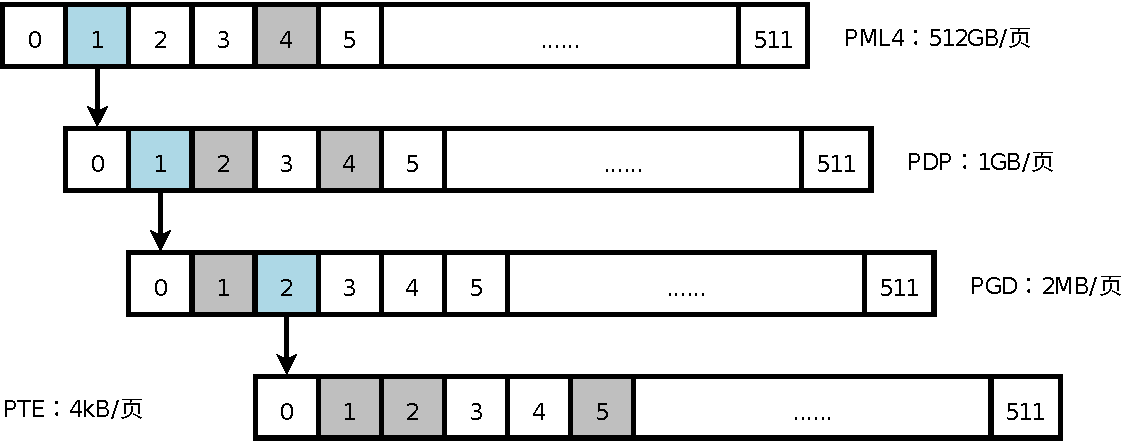
\includegraphics[width=0.72\textwidth]{Figure/image8.pdf}
    \caption{正常多级页表的例子}
    \label{fig:3-1-normal-multilevel-page-table-example}
\end{figure}

此外，如果允许一个页目录被构造进更高级页目录的任意虚拟地址槽位\footnote{只要大小和数量级数合适}，那么我们可以将内核配置为不检查起始虚拟地址是否合适。此时，我们使用的是正常多级页表，无需实现路径压缩。

由于处理器具备直接处理页表的硬件，因此我们不需要专门针对处理器生成页表元数据。但是需要注意，调用页表创建功能时，创建的页表应该合乎硬件页表查找机制的要求。对于那些纯软件填充TLB的MMU，则没有这个要求了，可以随意创建逻辑上符合页表形式的树结构，也可以把它们看成是基于区域的MMU，按照\ref{subsec:3-path-compressed-page-table-under-mpu}
所述的办法解决。

一些常见的MMU的特性如下：

\begin{xltabular}{\textwidth}{@{}>{\hsize=0.8979\hsize\raggedright\arraybackslash}X>{\hsize=0.6440\hsize\raggedright\arraybackslash}X>{\hsize=1.4399\hsize\raggedright\arraybackslash}X>{\hsize=1.0182\hsize\raggedright\arraybackslash}X@{}}
\caption{常见MMU的特性}\label{tab:3-4-common-mmu-features}\\
\toprule
处理器 & 页表级数 & 页大小 & 其他特性\tabularnewline
\endfirsthead
\toprule
处理器 & 页表级数 & 页大小 & 其他特性\tabularnewline
\midrule
\endhead
\bottomrule
\endlastfoot
ARM926EJ-S & 2或3级 & 1MB，64kB，4kB，1kB &
TLB部分表项手动锁定\tabularnewline
x86-64（AMD64） & 3级 & 1GB，2MB，4kB &
额外的段式内存管理单元\tabularnewline
Itanium（IA-64） & 4级 & 256MB，16MB，4MB，1MB，256kB，64kB，8kB，4kB &
可部分手动填充的TLB\tabularnewline
e200（PowerPC） & 不适用 & 1kB-4GB的所有2的次方 &
纯软件填充的TLB\tabularnewline
ARMv7-A（32-bit） & 2或3级 & 4kB，64kB，1MB，16MB &
TLB部分表项手动锁定\tabularnewline
ARMv8-M（64-bit） & 3或4级 & 4kB，16kB，64kB &
虚拟化下可选的2阶转换\tabularnewline
MIPS64 & 不适用 & 1kB-256MB的所有4的次方 &
纯软件填充的TLB\tabularnewline
TMS320C66X & 不适用 & 4kB-4GB的所有2的次方 &
纯软件填充的TLB\tabularnewline
\end{xltabular}

\subsection{内存保护单元下路径压缩页表的实现}\label{subsec:3-path-compressed-page-table-under-mpu}

在内存保护单元\footnote{或者手动填充的、基于区域的内存管理单元，下同}下，处理器往往不能直接识别多层的页表。这使得我们必须从页表生成MPU元数据用来在进程切换时高效地设置MPU。而且，在MPU环境下，还有如下的几个特点：

\begin{enumerate}
\def\labelenumi{\arabic{enumi}.}
\item
  MPU的区域个数往往是有限的，比如ARMv7-M有最多16个区域，每个区域又可以划分为8个子区域。因此，我们在一个进程中最多只能允许同时映射128个区域，而且这些区域还要满足一系列地址对齐等苛刻条件。因此，我们可以考虑把页分成两类，一类是静态页，它们总是被映射，要求可预测性的应用可以使用它们，静态页的最大数目就是处理器允许的最大MPU区域个数；另一类是动态页，它们只在使用时被映射，不保证在任何时候都被映射，动态页的最大数目是没有限制的。如果访问到了一个当前没有映射的动态页，那么处理器会进入缺页中断，然后我们手动查找页表来将该动态页加入MPU元数据，此时如果MPU区域不够可能会替换掉其他的动态页\hyperref[cite:3-2]{{[}2{]}}。
\item
  在一个页表里面，往往只有一两项是存在的。对于使用MPU的微控制器而言，维持多级页表的存在是没有必要的资源浪费，因此应该想办法对页表进行压缩。压缩页表和通常的页表相比，同一个页目录的不同中间页表项转换的地址位数可以是不同的。比如，在某个虚拟地址处，有一个很小的页，我们需要把它添加进访问范围。对于通常的页表，我们需要多级中间页目录，然后在最后一级页目录处，将这个页添加进去。而对于压缩页表，我们只要一级页目录就足以寻址该页。我们可以注明这个页目录的起始地址，数量级数和大小级数，然后直接将其构造进上级页目录中。当然，此时我们要求这一级页表所表示的虚拟地址范围落在上一级页目录的相应页表项允许的虚拟地址范围内。上述情况有一个例外：当架构实际上具备基于区域的MMU单元时，我们通常不使用路径压缩页表。
\item
  MPU不能进行物理地址到虚拟地址的转换。因此，虚拟地址总是等于物理地址的。这使得我们在映射页时必须检查页的映射地址是否等于物理地址。
\item
  由于我们需要MPU元数据来加速MPU填充，因此当我们修改任何一级页目录时，我们都必须维持元数据和页表的一致性。不维持这种一致性也是可以的，不过如果如此我们就只能通过缺页中断来更新元数据。而通过缺页中断来更新元数据并不总是可能的：部分架构在部分或全部情况下不提供缺页地址等关键信息。关于这种做法的详细信息请参看\ref{subsubsec:3-update-mpu-metadata-on-page-fault}
  。

  一个ARMv7-M上的路径压缩页表的例子如下图所示。绿色槽位代表路径压缩的指向子页目录的条目，蓝色槽位代表非路径压缩的指向子页目录的条目，而灰色槽位则代表被映射的页。各级页表前面的十六进制数代表了该页表的起始映射地址。

\begin{figure}[htbp]
    \centering
    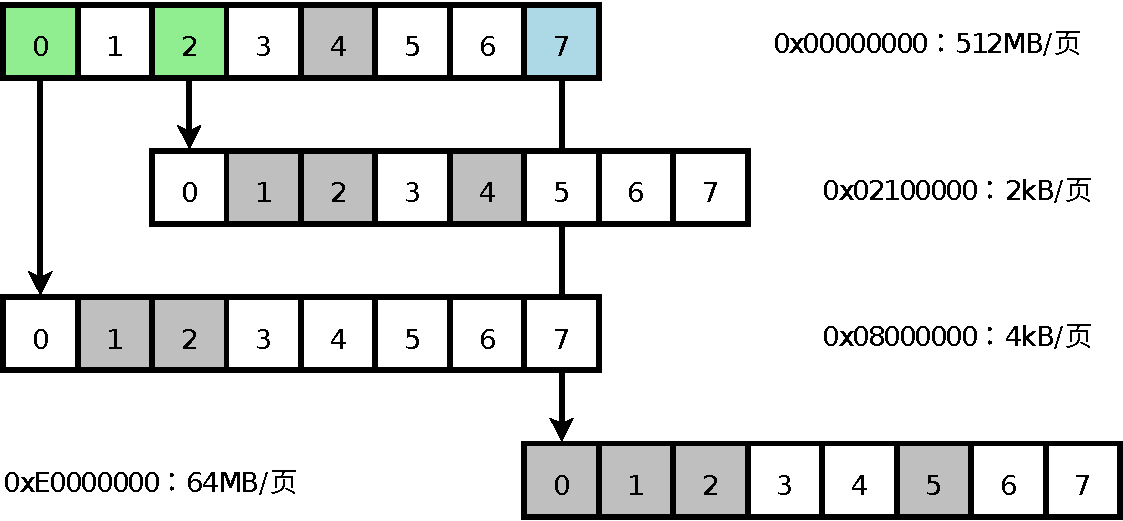
\includegraphics[width=0.72\textwidth]{Figure/image9.pdf}
    \caption{路径压缩页表的例子}
    \label{fig:3-2-path-compressed-page-table-example}
\end{figure}

  一些常见的MPU的特性如下：
\end{enumerate}

\begin{xltabular}{\textwidth}{@{}>{\hsize=1.0901\hsize\raggedright\arraybackslash}X>{\hsize=0.8740\hsize\raggedright\arraybackslash}X>{\hsize=1.1654\hsize\raggedright\arraybackslash}X>{\hsize=0.8740\hsize\raggedright\arraybackslash}X>{\hsize=0.9663\hsize\raggedright\arraybackslash}X>{\hsize=1.0301\hsize\raggedright\arraybackslash}X@{}}
\caption{常见MPU的特性}\label{tab:3-5-common-mpu-features}\\
\toprule
处理器 & 区域数量 & 区域组织 & 大小范围 & 对齐要求 &
其他特性\tabularnewline
\endfirsthead
\toprule
处理器 & 区域数量 & 区域组织 & 大小范围 & 对齐要求 &
其他特性\tabularnewline
\midrule
\endhead
\bottomrule
\endlastfoot
ARM v6-M & 0到16个 & 统一组织 & 128B-4GB & 对齐到大小 &
8个子区域\tabularnewline
ARM v7-M & 0到16个 & 统一组织 & 128B-4GB & 对齐到大小 &
8个子区域\tabularnewline
ARM v8-M & 0到16个 & 统一组织 & 128B-4GB & 无 & 无\tabularnewline
Tensilica L106 & 16或32个 & 统一组织 & 4kB-1GB & 无 & 无\tabularnewline
MIPS M14k & 1到16个 & 统一组织 & 任意 & 无 & 可锁定为只读\tabularnewline
PowerPC e200z4 & 32个 & 代码/数据各16个 & 任意 & 无 & 无\tabularnewline
AVR32 & 8个 & 统一组织 & 4kB-4GB & 对齐到大小 &
16个子区域\tabularnewline
MSP430FRXX & 3个 & 统一组织 & 任意 & 无 & 三段分段式\tabularnewline
Coldfire-MCF & 4个 & 代码/数据各2个 & 16MB-4GB & 对齐到大小 &
无\tabularnewline
RISC-V & 0到16个 & 统一组织 & 4B-4GB & 对齐到大小 &
也可对齐到字\tabularnewline
\end{xltabular}

综上所述，对于MPU下页表的实现，常见的有以下两种形式：

\subsubsection{更新页表时立即更新MPU元数据}\label{subsubsec:3-update-mpu-metadata-immediately}

这种做法仅仅把MPU元数据放置在顶层页目录中，而且要求构造时从顶层构造起。如果任何一级页目录没有顶层页目录，自己也不是顶层页目录，那么就无法构造子页目录到这个页目录之内。此外，任意两个页表都不能共享页目录或页目录树。这种实现的制约如下：

\begin{xltabular}{\textwidth}{@{}>{\hsize=0.5941\hsize\raggedright\arraybackslash}X>{\hsize=1.4059\hsize\raggedright\arraybackslash}X@{}}
\caption{更新页表时立即更新MPU元数据的制约}\label{tab:3-6-immediate-mpu-metadata-update-constraints}\\
\toprule
操作 & 制约或缺点\tabularnewline
\endfirsthead
\toprule
操作 & 制约或缺点\tabularnewline
\midrule
\endhead
\bottomrule
\endlastfoot
创建进程 & 无制约。\tabularnewline
更换进程页表 & 无制约。\tabularnewline
切换进程 & 无制约，直接使用顶层页目录中的MPU元数据即可。\tabularnewline
创建页目录 & 无制约。\tabularnewline
删除页目录 & 无制约。\tabularnewline
映射内存页 &
如果自己有顶层页目录，更新顶层页目录的MPU元数据。\tabularnewline
移除内存页 &
如果自己有顶层页目录，更新顶层页目录的MPU元数据。\tabularnewline
构造页目录 &
父页目录自己必须有顶层页目录，或者自己是顶层页目录；子页目录必须没有顶层页目录，而且自己不是顶层页目录\footnote{而且也不可能有子页目录}。添加子页目录的已映射页面到顶层页目录的MPU元数据。\tabularnewline
析构页目录 &
子页目录必须有顶层页目录，而且自己不得含有任何子页目录\footnote{其子页目录必须从本页目录中提前析构}。从顶层页目录的MPU元数据中移除子页目录的已映射页面。\tabularnewline
内存消耗 & 仅在顶层页目录有MPU元数据。\tabularnewline
\end{xltabular}

这个实现是单核系统上推荐的实现。这个实现最大限度地提高了基于MPU的微控制器的效率，使得我们往往能使用提前生成的MPU元数据批量设置MPU寄存器，而仅有一些不常用的功能的损失。当页表结构变化时，其MPU元数据也总是立即得到更新，不存在缺页中断引发的潜在实时性问题。

在某些架构上，有时\footnote{如ARMv7-M：它在硬件压栈和弹栈时的产生的缺页中断不提供缺页地址，因此不可将动态页用于栈}或总是\footnote{如ARMv6-M：由于极度精简，它在任何情况下都不提供任何异常处理信息，因此完全不支持动态页}无法在缺页中断中确定缺页地址，无法根据地址来动态映射页面。此类架构因为缺乏异常处理信息，在某些或全部情况下不支持动态页。

\subsubsection{缺页中断时更新MPU元数据}\label{subsubsec:3-update-mpu-metadata-on-page-fault}

这种做法把放置在顶层页目录处的MPU的元数据看作是软件填充的TLB，使用在内存保护中断中的软件页表遍历算法来在每次不命中时填充它。它不试图一次生成整个页表对应的MPU元数据，而是选择逐步生成它。在每次页表结构变化或页映射变化时，清空所有的MPU元数据，这相当于MMU架构下的TLB刷新。这种做法也支持静态页和动态页，并且静态页只在第一次访问时会出现缺页中断，后续访问则可以保证实时性。

\begin{xltabular}{\textwidth}{@{}>{\hsize=0.8054\hsize\raggedright\arraybackslash}X>{\hsize=1.1946\hsize\raggedright\arraybackslash}X@{}}
\caption{缺页中断时更新MPU元数据的制约}\label{tab:3-7-page-fault-mpu-metadata-update-constraints}\\
\toprule
操作 & 制约或缺点\tabularnewline
\endfirsthead
\toprule
操作 & 制约或缺点\tabularnewline
\midrule
\endhead
\bottomrule
\endlastfoot
创建进程 & 无制约。\tabularnewline
更换进程页表 & 清空MPU元数据，准备重建。\tabularnewline
切换进程 & 无制约。\tabularnewline
创建页目录 & 无制约。\tabularnewline
删除页目录 & 无制约。\tabularnewline
映射内存页 & 无制约。\tabularnewline
移除内存页 & 清空MPU元数据，准备重建。\tabularnewline
构造页目录 & 无制约。\tabularnewline
析构页目录 & 清空MPU元数据，准备重建。\tabularnewline
内存消耗 & 仅在顶层页目录有MPU元数据。\tabularnewline
\end{xltabular}

这个实现保留了和MMU系统最大的兼容性，也是多核MPU架构上推荐的实现方法。它对页表的构造顺序没有要求，也方便在多核环境下进行操作，而且多个页表可以以任意方式共享一部分，但其实时性能比\ref{subsubsec:3-update-mpu-metadata-immediately}
中列出的方案稍差。

\needspace{30\baselineskip}
\section{页表功能列表}\label{sec:3-page-table-function-list}
\nopagebreak[4]

\needspace{20\baselineskip}
与页表有关的内核功能如下：

\begin{xltabular}{\textwidth}{@{}>{\hsize=1.1605\hsize\raggedright\arraybackslash}X>{\hsize=0.8843\hsize\raggedright\arraybackslash}X>{\hsize=0.9552\hsize\raggedright\arraybackslash}X@{}}
\caption{页表相关内核功能}\label{tab:3-8-page-table-related-kernel-functions}\\
\toprule
调用号 & 类型 & 用途\tabularnewline
\endfirsthead
\toprule
调用号 & 类型 & 用途\tabularnewline
\midrule
\endhead
\bottomrule
\endlastfoot
RME\_SVC\_PGT\_CRT & 系统调用 & 创建页目录\tabularnewline
RME\_SVC\_PGT\_DEL & 系统调用 & 删除页目录\tabularnewline
RME\_SVC\_PGT\_ADD & 系统调用 & 映射内存页\tabularnewline
RME\_SVC\_PGT\_REM & 系统调用 & 移除内存页\tabularnewline
RME\_SVC\_PGT\_CON & 系统调用 & 构造页目录\tabularnewline
RME\_SVC\_PGT\_DES & 系统调用 & 析构页目录\tabularnewline
\end{xltabular}

页表权能的操作标志如下：

\begin{xltabular}{\textwidth}{@{}>{\hsize=1.0017\hsize\raggedright\arraybackslash}X>{\hsize=0.6199\hsize\raggedright\arraybackslash}X>{\hsize=1.3784\hsize\raggedright\arraybackslash}X@{}}
\caption{页表操作标志}\label{tab:3-9-page-table-operation-flags}\\
\toprule
标志 & 位 & 用途\tabularnewline
\endfirsthead
\toprule
标志 & 位 & 用途\tabularnewline
\midrule
\endhead
\bottomrule
\endlastfoot
RME\_PGT\_FLAG\_ADD\_SRC & {[}0{]} &
允许该页目录在页框传递作为来源目录。\tabularnewline
RME\_PGT\_FLAG\_ADD\_DST & {[}1{]} &
允许该页目录在权能传递作为目标目录。\tabularnewline
RME\_PGT\_FLAG\_REM & {[}2{]} &
允许移除该页目录中的页框。\tabularnewline
RME\_PGT\_FLAG\_CHILD & {[}3{]} &
允许该页目录在页表构造或析构中作为子页目录。\tabularnewline
RME\_PGT\_FLAG\_CON\_PARENT & {[}4{]} &
允许该页目录在页表构造中作为父页目录。\tabularnewline
RME\_PGT\_FLAG\_DES\_PARENT & {[}5{]} &
允许该页目录在页表析构中作为父页目录。\tabularnewline
RME\_PGT\_FLAG\_PRC\_CRT & {[}6{]} &
允许在创建进程时将该页表作为进程的页表。\tabularnewline
RME\_PGT\_FLAG\_PRC\_PGT & {[}7{]} &
允许用该页表替换某进程的页表。\tabularnewline
其他位 & 位段 & 操作范围属性。\tabularnewline
\end{xltabular}

关于上表中的位{[}6{]}和位{[}7{]}，请参看\ref{subsec:4-create-a-process}
和\ref{subsec:4-change-process-capability-table}
。在页表相关内核功能中填充操作标志时，要使用 RME\_PGT\_FLAG(HIGH,LOW,FLAG) 宏进行填充，其中 HIGH 为操作位置 Pos 的上限，LOW 为操作位置 Pos 的下限，[HIGH, LOW] 组成的闭区间即为允许的 Pos 范围。FLAG 则为位{[}7:0{]}中各个被允许的操作标志。

\subsection{创建页目录}\label{subsec:3-create-page-directory}

该操作会创建一个页目录，并将其权能放入某个已存在的权能表。创建页目录操作需要如下几个参数：

\begin{xltabular}{\textwidth}{@{}>{\hsize=0.7362\hsize\raggedright\arraybackslash}X>{\hsize=0.6815\hsize\raggedright\arraybackslash}X>{\hsize=0.6815\hsize\raggedright\arraybackslash}X>{\hsize=1.9007\hsize\raggedright\arraybackslash}X@{}}
\caption{创建页目录的所需参数}\label{tab:3-10-create-page-directory-parameters}\\
\toprule
参数名称 & 类型 & 域 & 描述\tabularnewline
\endfirsthead
\toprule
参数名称 & 类型 & 域 & 描述\tabularnewline
\midrule
\endhead
\bottomrule
\endlastfoot
Svc\_Num & ptr\_t & N.Q0 & 必须为 RME\_SVC\_PGT\_CRT。\tabularnewline
Cap\_Cpt & cid\_t & C &
一个对应于必须拥有 RME\_CPT\_FLAG\_CRT 属性的权能表权能的权能号，该权能号对应的权能指向要接受此新创建的页目录权能的权能表。该权能号可以是一级或者二级查找编码。\tabularnewline
Cap\_Kom & cid\_t & P1.D1 &
一个内核内存权能号，其标识的内核内存范围必须能够放下整个页目录，并且要拥有 RME\_KOM\_FLAG\_PGT 属性。该权能号可以是一级或二级查找编码。\tabularnewline
Cap\_Pgt & cid\_t & P1.Q1 &
一个对应于接受该新创建的页目录权能的权能表的某位置的权能号。该权能号对应的权能必须是空白的。该权能号只能是一级查找编码。\tabularnewline
Raddr & ptr\_t & P2 &
新创建的页目录要使用的内核起始相对虚拟地址。这个地址是相对于Cap\_Kom对应的内核权能的起始虚拟地址的。\tabularnewline
Base & ptr\_t & P3 &
新创建的页目录的映射起始地址，最后一位为顶层标志，见下。\tabularnewline
Is\_Top & ptr\_t & P3{[}0{]} &
该页目录是否是顶层页目录。``1''意味着该页目录为顶层。\tabularnewline
Size\_Order & ptr\_t & P1.Q0 &
该页目录的大小级数\footnote{指每个页表项代表的内存页大小}。\tabularnewline
Num\_Order & ptr\_t & N.Q1 & 该页目录的数目级数。\tabularnewline
\end{xltabular}

该操作的返回值可能如下：

\begin{xltabular}{\textwidth}{@{}>{\hsize=0.8188\hsize\raggedright\arraybackslash}X>{\hsize=1.1812\hsize\raggedright\arraybackslash}X@{}}
\caption{创建页目录的可能返回值}\label{tab:3-11-create-page-directory-return-values}\\
\toprule
返回值 & 意义\tabularnewline
\endfirsthead
\toprule
返回值 & 意义\tabularnewline
\midrule
\endhead
\bottomrule
\endlastfoot
    0 & 操作成功。\tabularnewline
    RME\_ERR\_CPT\_RANGE & Cap\_Cpt 的一级/二级查找超出了范围。\tabularnewline
    RME\_ERR\_CPT\_RANGE & Cap\_Kom 的一级/二级查找超出了范围。\tabularnewline
    RME\_ERR\_CPT\_RANGE & Cap\_Pgt 的一级查找超出了范围。\tabularnewline
    RME\_ERR\_CPT\_FROZEN & Cap\_Cpt 的一级/二级查找的权能已经被冻结。\tabularnewline
    RME\_ERR\_CPT\_FROZEN & Cap\_Kom 的一级/二级查找的权能已经被冻结。\tabularnewline
    RME\_ERR\_CPT\_FROZEN & Cap\_Pgt 被冻结，或者其它核正在该处创建权能。\tabularnewline
    RME\_ERR\_CPT\_TYPE & Cap\_Cpt 不是权能表权能。\tabularnewline
    RME\_ERR\_CPT\_TYPE & Cap\_Kom 不是内核内存权能。\tabularnewline
    RME\_ERR\_CPT\_FLAG & Cap\_Cpt 无 RME\_CPT\_FLAG\_CRT 属性。\tabularnewline
    RME\_ERR\_CPT\_FLAG & Cap\_Kom 无 RME\_KOM\_FLAG\_PGT 属性，或范围错误。\tabularnewline
    RME\_ERR\_CPT\_EXIST & Cap\_Pgt 不是空白权能。\tabularnewline
    RME\_ERR\_CPT\_KOT & 分配内核内存失败。\tabularnewline
    RME\_ERR\_PGT\_HW & 底层硬件制约，不允许创建这样的页目录。\tabularnewline
\end{xltabular}

\needspace{30\baselineskip}
\subsection{删除页目录}\label{subsec:3-delete-page-directory}
\nopagebreak[4]

该操作会删除一个页目录。被删除的页目录必须不含有子页目录。删除页目录需要以下几个参数：

\begin{xltabular}{\textwidth}{@{}>{\hsize=0.6910\hsize\raggedright\arraybackslash}X>{\hsize=0.6910\hsize\raggedright\arraybackslash}X>{\hsize=0.6910\hsize\raggedright\arraybackslash}X>{\hsize=1.9271\hsize\raggedright\arraybackslash}X@{}}
\caption{删除页目录的所需参数}\label{tab:3-12-delete-page-directory-parameters}\\
\toprule
参数名称 & 类型 & 域 & 描述\tabularnewline
\endfirsthead
\toprule
参数名称 & 类型 & 域 & 描述\tabularnewline
\midrule
\endhead
\bottomrule
\endlastfoot
Svc\_Num & ptr\_t & N & 必须为 RME\_SVC\_PGT\_DEL。\tabularnewline
Cap\_Cpt & cid\_t & C &
一个对应于必须拥有 RME\_CPT\_FLAG\_DEL 属性的权能表权能的权能号，该权能号对应的权能指向含有正被删除的页目录权能的权能表。该权能号可以是一级或者二级查找编码。\tabularnewline
Cap\_Pgt & cid\_t & P1 &
一个对应于将被删除的页目录权能的权能号。该权能号对应的权能必须是一个页目录权能。该权能号只能是一级查找编码。\tabularnewline
\end{xltabular}

该操作的返回值可能如下：

\begin{xltabular}{\textwidth}{@{}>{\hsize=0.6791\hsize\raggedright\arraybackslash}X>{\hsize=1.3209\hsize\raggedright\arraybackslash}X@{}}
\caption{删除页目录的可能返回值}\label{tab:3-13-delete-page-directory-return-values}\\
\toprule
返回值 & 意义\tabularnewline
\endfirsthead
\toprule
返回值 & 意义\tabularnewline
\midrule
\endhead
\bottomrule
\endlastfoot
    0 & 操作成功。\tabularnewline
    RME\_ERR\_CPT\_RANGE & Cap\_Cpt 的一级/二级查找超出了范围。\tabularnewline
    RME\_ERR\_CPT\_RANGE & Cap\_Pgt 的一级查找超出了范围。\tabularnewline
    RME\_ERR\_CPT\_FROZEN & Cap\_Cpt 的一级/二级查找的权能已经被冻结。\tabularnewline
    RME\_ERR\_CPT\_FROZEN & Cap\_Pgt 未被冻结。\tabularnewline
    RME\_ERR\_CPT\_TYPE & Cap\_Cpt 不是权能表权能。\tabularnewline
    RME\_ERR\_CPT\_TYPE & Cap\_Pgt 不是页目录权能。\tabularnewline
    RME\_ERR\_CPT\_NULL & Cap\_Pgt 为空白权能。\tabularnewline
    RME\_ERR\_CPT\_NULL & 两个核同时试图删除该页目录，此时未成功的核返回该值。\tabularnewline
    RME\_ERR\_CPT\_FLAG & Cap\_Cpt 无 RME\_CPT\_FLAG\_DEL 属性。\tabularnewline
    RME\_ERR\_CPT\_QUIE & Cap\_Pgt 不安定。\tabularnewline
    RME\_ERR\_CPT\_REFCNT & Cap\_Pgt 的引用计数不为 0，或者不为根权能。\tabularnewline
    RME\_ERR\_PGT\_HW & 底层硬件制约，不允许删除这个页目录。这可能是因为页目录中含有子页目录或者等等其他原因。\tabularnewline
\end{xltabular}

\subsection{映射内存页}\label{subsec:3-map-memory-page}

该操作会将一个页目录中的某个页表项的某一部分传递到另外一个页目录的空白位置中。在页目录之间进行页表项传递需要以下几个参数：

\begin{xltabular}{\textwidth}{@{}>{\hsize=0.7639\hsize\raggedright\arraybackslash}X>{\hsize=0.6758\hsize\raggedright\arraybackslash}X>{\hsize=0.6758\hsize\raggedright\arraybackslash}X>{\hsize=1.8846\hsize\raggedright\arraybackslash}X@{}}
\caption{映射内存页的所需参数}\label{tab:3-14-map-memory-page-parameters}\\
\toprule
参数名称 & 类型 & 域 & 描述\tabularnewline
\endfirsthead
\toprule
参数名称 & 类型 & 域 & 描述\tabularnewline
\midrule
\endhead
\bottomrule
\endlastfoot
Svc\_Num & ptr\_t & N & 必须为 RME\_SVC\_PGT\_ADD。\tabularnewline
Cap\_Pgt\_Dst & cid\_t & P1.D1 &
一个对应于必须拥有 RME\_PGT\_FLAG\_ADD\_DST 属性的页目录权能的权能号，该权能号对应的权能指向目标页目录。该权能号可以是一级或者二级查找编码。\tabularnewline
Pos\_Dst & ptr\_t & P1.D0 &
一个该目标页目录中要接受传递的目标页表项位置。该页表项必须是空白的。\tabularnewline
Flag\_Dst & ptr\_t & C &
目标页表项的属性。这个属性限制了目标页表项的特性。\tabularnewline
Cap\_Pgt\_Src & cid\_t & P2.D1 &
一个对应于必须拥有 RME\_PGT\_FLAG\_ADD\_SRC 属性的页目录权能的权能号，该权能号对应的权能指向源页目录。该权能号可以是一级或者二级查找编码。\tabularnewline
Pos\_Src & ptr\_t & P2.D0 &
一个源页目录中要被传递的源页框位置。该页框必须是被映射的。\tabularnewline
Index & ptr\_t & P3 & 要被传递的源页框中的子位置。\tabularnewline
\end{xltabular}

该操作的返回值可能如下：

\begin{xltabular}{\textwidth}{@{}>{\hsize=0.6791\hsize\raggedright\arraybackslash}X>{\hsize=1.3209\hsize\raggedright\arraybackslash}X@{}}
\caption{映射内存页的可能返回值}\label{tab:3-15-map-memory-page-return-values}\\
\toprule
返回值 & 意义\tabularnewline
\endfirsthead
\toprule
返回值 & 意义\tabularnewline
\midrule
\endhead
\bottomrule
\endlastfoot
    0 & 操作成功。\tabularnewline
    RME\_ERR\_CPT\_RANGE & Cap\_Pgt\_Dst 或 Cap\_Pgt\_Src 的一级/二级查找超出了范围。\tabularnewline
    RME\_ERR\_CPT\_FROZEN & Cap\_Pgt\_Dst 或 Cap\_Pgt\_Src 的一级/二级查找的权能被冻结。\tabularnewline
    RME\_ERR\_CPT\_TYPE & Cap\_Pgt\_Dst 或 Cap\_Pgt\_Src 不是页目录权能。\tabularnewline
    RME\_ERR\_CPT\_FLAG & Cap\_Pgt\_Src 无 RME\_PGT\_FLAG\_ADD\_SRC 属性。\tabularnewline
    RME\_ERR\_CPT\_FLAG & Cap\_Pgt\_Dst 无 RME\_PGT\_FLAG\_ADD\_DST 属性。\tabularnewline
    RME\_ERR\_CPT\_FLAG & Cap\_Pgt\_Dst 或 Cap\_Pgt\_Src 的操作范围属性不允许该操作。\tabularnewline
    RME\_ERR\_PGT\_ADDR & 目标页目录的大小级数比源页目录的大小级数大，因此不能映射。\tabularnewline
    RME\_ERR\_PGT\_ADDR & Pos\_Dst 或 Pos\_Src 超出了目标页目录或者源页目录的页表项数目。\tabularnewline
    RME\_ERR\_PGT\_ADDR & Index 超出了子位置的最大编号。\tabularnewline
    RME\_ERR\_PGT\_ADDR & 在开启了物理地址等于虚拟地址的检查时，映射的物理地址和目标虚拟地址不同。\tabularnewline
    RME\_ERR\_PGT\_HW & 源页目录查找失败。这可能是由于源页目录的该位置为空。\tabularnewline
    RME\_ERR\_PGT\_MAP & 尝试映射，由于硬件原因失败。具体的失败原因与硬件有关。\tabularnewline
    RME\_ERR\_PGT\_PERM & 目标页的访问控制标志不是源页的访问控制标志的子集。\tabularnewline
\end{xltabular}

\subsection{移除内存页}\label{subsec:3-remove-memory-page}

该操作会将一个页目录中的某个页表项除去，使该位回归空白状态。移除内存页需要如下参数：

\begin{xltabular}{\textwidth}{@{}>{\hsize=0.6910\hsize\raggedright\arraybackslash}X>{\hsize=0.6910\hsize\raggedright\arraybackslash}X>{\hsize=0.6910\hsize\raggedright\arraybackslash}X>{\hsize=1.9271\hsize\raggedright\arraybackslash}X@{}}
\caption{移除内存页的所需参数}\label{tab:3-16-remove-memory-page-parameters}\\
\toprule
参数名称 & 类型 & 域 & 描述\tabularnewline
\endfirsthead
\toprule
参数名称 & 类型 & 域 & 描述\tabularnewline
\midrule
\endhead
\bottomrule
\endlastfoot
Svc\_Num & ptr\_t & N & 必须为 RME\_SVC\_PGT\_REM。\tabularnewline
Cap\_Pgt & cid\_t & P1 &
一个对应于必须拥有 RME\_PGT\_FLAG\_REM 属性的页目录权能的权能号，该权能号对应的权能指向目标页目录。该权能号可以是一级或者二级查找编码。\tabularnewline
Pos & ptr\_t & P2 &
一个该目标页目录中要除去的页表项位置。该页表项必须是一个被映射的内存页。\tabularnewline
\end{xltabular}

\needspace{20\baselineskip}
该操作的返回值可能如下：

\begin{xltabular}{\textwidth}{@{}>{\hsize=0.7363\hsize\raggedright\arraybackslash}X>{\hsize=1.2637\hsize\raggedright\arraybackslash}X@{}}
\caption{移除内存页的可能返回值}\label{tab:3-17-remove-memory-page-return-values}\\
\toprule
返回值 & 意义\tabularnewline
\endfirsthead
\toprule
返回值 & 意义\tabularnewline
\midrule
\endhead
\bottomrule
\endlastfoot
    0 & 操作成功。\tabularnewline
    RME\_ERR\_CPT\_RANGE & Cap\_Pgt 的一级/二级查找超出了范围。\tabularnewline
    RME\_ERR\_CPT\_FROZEN & Cap\_Pgt 的一级/二级查找的权能被冻结。\tabularnewline
    RME\_ERR\_CPT\_TYPE & Cap\_Pgt 不是页目录权能。\tabularnewline
    RME\_ERR\_CPT\_FLAG & Cap\_Pgt 无 RME\_PGT\_FLAG\_REM 属性。\tabularnewline
    RME\_ERR\_CPT\_FLAG & Cap\_Pgt 的操作范围属性不允许该操作。\tabularnewline
    RME\_ERR\_PGT\_ADDR & Pos 超出了目标页目录的页表项数目。\tabularnewline
    RME\_ERR\_PGT\_MAP & 尝试除去，由于硬件原因失败。具体的失败原因与硬件有关。\tabularnewline
\end{xltabular}

\subsection{构造页目录}\label{subsec:3-construct-page-directory}

该操作会将指向子页目录的物理地址指针放入父页目录的某个空白位置之中。如果使用压缩页表，子页目录的大小必须小于等于父页目录的一个页，否则子页目录的大小必须正好等于父页目录的一个页。构造页目录需要如下参数：

\begin{xltabular}{\textwidth}{@{}>{\hsize=0.7600\hsize\raggedright\arraybackslash}X>{\hsize=0.5600\hsize\raggedright\arraybackslash}X>{\hsize=0.5600\hsize\raggedright\arraybackslash}X>{\hsize=2.1200\hsize\raggedright\arraybackslash}X@{}}
\caption{构造页目录的所需参数}\label{tab:3-18-construct-page-directory-parameters}\\
\toprule
参数名称 & 类型 & 域 & 描述\tabularnewline
\endfirsthead
\toprule
参数名称 & 类型 & 域 & 描述\tabularnewline
\midrule
\endhead
\bottomrule
\endlastfoot
    Svc\_Num & ptr\_t & N & 必须为 RME\_SVC\_PGT\_CON。\tabularnewline
    Cap\_Pgt\_Parent & cid\_t & P1.D1 & 一个对应于必须拥有 RME\_PGT\_FLAG\_CON\_PARENT 属性的页目录权能的权能号，该权能号对应的权能指向父页目录。该权能号可以是一级或者二级查找编码。\tabularnewline
    Pos & ptr\_t & P2 & 一个该目标页目录中要接受传递的目标页表项位置。该页表项必须是空白的。\tabularnewline
    Cap\_Pgt\_Child & cid\_t & P1.D0 & 一个对应于必须拥有 RME\_PGT\_FLAG\_CHILD 属性的页目录权能的权能号，该权能号对应的权能指向子页目录。该权能号可以是一级或者二级查找编码。\tabularnewline
    Flag\_Child & ptr\_t & P3 & 子页目录被映射时的属性。这个属性限制了该映射以下的所有页目录的访问权限。对于不同的架构，这个位置的值的意义也不相同。对于有些不支持页目录属性的架构，这个值无效。\tabularnewline
\end{xltabular}

该操作的返回值可能如下：

\begin{xltabular}{\textwidth}{@{}>{\hsize=0.6791\hsize\raggedright\arraybackslash}X>{\hsize=1.3209\hsize\raggedright\arraybackslash}X@{}}
\caption{构造页目录的可能返回值}\label{tab:3-19-construct-page-directory-return-values}\\
\toprule
返回值 & 意义\tabularnewline
\endfirsthead
\toprule
返回值 & 意义\tabularnewline
\midrule
\endhead
\bottomrule
\endlastfoot
    0 & 操作成功。\tabularnewline
    RME\_ERR\_CPT\_RANGE & Cap\_Pgt\_Parent 或 Cap\_Pgt\_Child 的一级/二级查找超出了范围。\tabularnewline
    RME\_ERR\_CPT\_FROZEN & Cap\_Pgt\_Parent 或 Cap\_Pgt\_Child 的一级/二级查找的权能被冻结。\tabularnewline
    RME\_ERR\_CPT\_TYPE & Cap\_Pgt\_Parent 或 Cap\_Pgt\_Child 不是页目录权能。\tabularnewline
    RME\_ERR\_CPT\_FLAG & Cap\_Pgt\_Parent 无 RME\_PGT\_FLAG\_CON\_PARENT 属性。\tabularnewline
    RME\_ERR\_CPT\_FLAG & Cap\_Pgt\_Child 无 RME\_PGT\_FLAG\_CHILD 属性。\tabularnewline
    RME\_ERR\_CPT\_FLAG & Cap\_Pgt\_Parent 的操作范围属性不允许该操作。\tabularnewline
    RME\_ERR\_PGT\_ADDR & Pos 超出了父页目录的页表项数目。\tabularnewline
    RME\_ERR\_PGT\_ADDR & 子页目录的总大小大于父页目录的一个页的大小。\tabularnewline
    RME\_ERR\_PGT\_ADDR & 在开启了物理地址等于虚拟地址的检查时\footnote{基于内存保护单元的架构，如 ARMv7-M}，映射的物理地址和目标虚拟地址不相等。\tabularnewline
    RME\_ERR\_PGT\_MAP & 尝试构造，由于硬件原因失败。具体的失败原因与硬件有关，可能是硬件不支持此种映射。\tabularnewline
\end{xltabular}

\subsection{析构页目录}\label{subsec:3-destruct-page-directory}

该操作会将一个页目录中的某个子页目录除去，使该位回归空白状态。析构页目录需要如下参数：

\begin{xltabular}{\textwidth}{@{}>{\hsize=0.8381\hsize\raggedright\arraybackslash}X>{\hsize=0.6603\hsize\raggedright\arraybackslash}X>{\hsize=0.6603\hsize\raggedright\arraybackslash}X>{\hsize=1.8414\hsize\raggedright\arraybackslash}X@{}}
\caption{析构页目录的所需参数}\label{tab:3-20-destruct-page-directory-parameters}\\
\toprule
参数名称 & 类型 & 域 & 描述\tabularnewline
\endfirsthead
\toprule
参数名称 & 类型 & 域 & 描述\tabularnewline
\midrule
\endhead
\bottomrule
\endlastfoot
Svc\_Num & ptr\_t & N & 必须为 RME\_SVC\_PGT\_DES。\tabularnewline
Cap\_Pgt\_Parent & cid\_t & P1 &
一个对应于必须拥有 RME\_PGT\_FLAG\_DES\_PARENT 属性的页目录权能的权能号，该权能号对应的权能指向父页目录。该权能号可以是一级或者二级查找编码。\tabularnewline
Pos & ptr\_t & P2 &
一个该目标页目录中要除去的子页目录位置。该页表项必须是一个被映射的页目录。\tabularnewline
Cap\_Pgt\_Child & cid\_t & P3 &
一个对应于必须拥有RME\_PGT\_FLAG\_CHILD属性的页目录权能的权能号，该权能号对应的权能指向子页目录。该子页目录必须位于父页目录的 Pos 处。该权能号可以是一级或者二级查找编码。\tabularnewline
\end{xltabular}

该操作的返回值可能如下：

\begin{xltabular}{\textwidth}{@{}>{\hsize=0.7199\hsize\raggedright\arraybackslash}X>{\hsize=1.2801\hsize\raggedright\arraybackslash}X@{}}
\caption{析构页目录的可能返回值}\label{tab:3-21-destruct-page-directory-return-values}\\
\toprule
返回值 & 意义\tabularnewline
\endfirsthead
\toprule
返回值 & 意义\tabularnewline
\midrule
\endhead
\bottomrule
\endlastfoot
    0 & 操作成功。\tabularnewline
    RME\_ERR\_CPT\_RANGE & Cap\_Pgt\_Parent或Cap\_Pgt\_Child的一级/二级查找超出了范围。\tabularnewline
    RME\_ERR\_CPT\_FROZEN & Cap\_Pgt\_Parent或Cap\_Pgt\_Child的一级/二级查找的权能被冻结。\tabularnewline
    RME\_ERR\_CPT\_TYPE & Cap\_Pgt\_Parent或Cap\_Pgt\_Child不是页目录权能。\tabularnewline
    RME\_ERR\_CPT\_FLAG & Cap\_Pgt\_Parent无RME\_PGT\_FLAG\_DES\_PARENT属性。\tabularnewline
    RME\_ERR\_CPT\_FLAG & Cap\_Pgt\_Child无RME\_PGT\_FLAG\_CHILD属性。\tabularnewline
    RME\_ERR\_PGT\_ADDR & Pos 超出了父页目录的页表项数目。\tabularnewline
    RME\_ERR\_PGT\_MAP & 尝试析构，由于硬件原因失败。具体的失败原因与硬件有关。\tabularnewline
\end{xltabular}

\needspace{30\baselineskip}
\section{内核内存功能列表}\label{sec:3-kernel-memory-function-list}
\nopagebreak[4]

与内核内存有关的内核功能只有一个，就是进行内核内存权能的传递。初始的内核内存权能是在系统启动时创建的，并且无法删除。其传递产生的子权能无法被删除，只能被移除。内核内存权能不仅有操作标志，还有一个对齐到64Byte的虚拟地址范围值。在所有的内核对象中，只有下表所列的四种内核对象需要内核内存。

\needspace{20\baselineskip}
内核内存权能的操作标志如下：

\begin{xltabular}{\textwidth}{@{}>{\hsize=0.9185\hsize\raggedright\arraybackslash}X>{\hsize=0.6784\hsize\raggedright\arraybackslash}X>{\hsize=1.4031\hsize\raggedright\arraybackslash}X@{}}
\caption{内核内存操作标志}\label{tab:3-22-kernel-memory-operation-flags}\\
\toprule
标志 & 位 & 用途\tabularnewline
\endfirsthead
\toprule
标志 & 位 & 用途\tabularnewline
\midrule
\endhead
\bottomrule
\endlastfoot
RME\_KOM\_FLAG\_CPT & {[}0{]} &
允许在该段内核内存上创建权能表。\tabularnewline
RME\_KOM\_FLAG\_PGT & {[}1{]} &
允许在该段内核内存上创建页目录。\tabularnewline
RME\_KOM\_FLAG\_THD & {[}2{]} &
允许在该段内核内存上创建线程。\tabularnewline
RME\_KOM\_FLAG\_INV & {[}3{]} &
允许在该段内核内存上创建同步迁移调用。\tabularnewline
\end{xltabular}

在进行内核内存权能的传递时，由于还需要传入一个范围参数，因此仅用一个参数位置 P3 是无法完全传递所需信息的。此时，需要使用系统调用号 N 的一部分和权能表权能号 C 来传递这些参数。具体的参数传递规则如下：

\begin{xltabular}{\textwidth}{@{}>{\hsize=0.7639\hsize\raggedright\arraybackslash}X>{\hsize=0.6758\hsize\raggedright\arraybackslash}X>{\hsize=0.6758\hsize\raggedright\arraybackslash}X>{\hsize=1.8846\hsize\raggedright\arraybackslash}X@{}}
\caption{内核内存权能传递的所需参数}\label{tab:3-23-kernel-memory-capability-transfer-parameters}\\
\toprule
参数名称 & 类型 & 域 & 描述\tabularnewline
\endfirsthead
\toprule
参数名称 & 类型 & 域 & 描述\tabularnewline
\midrule
\endhead
\bottomrule
\endlastfoot
Svc\_Num & ptr\_t & N{[}5:0{]} & 必须为 RME\_SVC\_CPT\_ADD。\tabularnewline
Cap\_Cpt\_Dst & cid\_t & P1.D1 &
一个对应于必须拥有 RME\_CPT\_FLAG\_ADD\_DST 属性的权能表权能的权能号，该权能号对应的权能指向目标权能表。该权能号可以是一级或者二级查找编码。\tabularnewline
Cap\_Dst & cid\_t & P1.D0 &
一个对应于将接受被传递的权能的权能号。该权能号对应的权能必须是空白的。该权能号只能是一级查找编码。\tabularnewline
Cap\_Cpt\_Src & cid\_t & P2.D1 &
一个对应于必须拥有 RME\_CPT\_FLAG\_ADD\_SRC 属性的权能表权能的权能号，该权能号对应的权能指向源权能表。该权能号可以是一级或者二级查找编码。\tabularnewline
Cap\_Src & cid\_t & P2.D0 &
一个对应于将传递的权能的权能号。该权能号对应的权能必须不为空白而且没有冻结。该权能号只能是一级查找编码。\tabularnewline
Flag & ptr\_t & P3 & 描述见下文。\tabularnewline
Ext\_Flag & ptr\_t & N:C & 描述见下文。\tabularnewline
\end{xltabular}

内核内存权能的传递中，P3 和 N:C 共同决定了新产生的内核内存权能的扩展操作标志属性。N:C 表示将半字 N 和半字 C 组合起来，其中 N 处于高半字，C 处于低半字，共同组成一个字。由于 RME 仅仅使用了 N 的最后 6 个二进制位表示系统调用号，因此剩余的二进制位可以被用来表示其他信息。N 和 C 组合起来一共有 X-6 个二进制位（X 为按照二进制位的数量计算的机器字长），加上 P3 提供的 X 个二进制位，一共有 2X-6 个二进制位。我们为操作标志保留 6 个二进制位，因此内核内存的上界和下界可以各分配 X-6 位，这正好能表示对齐到 64 字节的内存地址。

\needspace{20\baselineskip}
P3（Flag）的具体意义如下：

\begin{xltabular}{\textwidth}{@{}>{\hsize=0.7396\hsize\raggedright\arraybackslash}X>{\hsize=1.2604\hsize\raggedright\arraybackslash}X@{}}
\caption{内核内存权能传递中P3（Flag）的具体含义}\label{tab:3-24-kernel-memory-p3-flag-meaning}\\
\toprule
位段范围 & 位段意义\tabularnewline
\endfirsthead
\toprule
位段范围 & 位段意义\tabularnewline
\midrule
\endhead
\bottomrule
\endlastfoot
高半字（D1） & 内核内存相对地址上限的高半字。\tabularnewline
低半字（D0） & 内核内存相对地址下限的高半字。\tabularnewline
\end{xltabular}

\needspace{20\baselineskip}
N:C（Ext\_Flag）的具体意义如下：

\begin{xltabular}{\textwidth}{@{}>{\hsize=0.8711\hsize\raggedright\arraybackslash}X>{\hsize=1.1289\hsize\raggedright\arraybackslash}X@{}}
\caption{内核内存权能传递中N:C（Ext\_Flag）的具体含义}\label{tab:3-25-kernel-memory-ext-flag-meaning}\\
\toprule
位段范围 & 位段意义\tabularnewline
\endfirsthead
\toprule
位段范围 & 位段意义\tabularnewline
\midrule
\endhead
\bottomrule
\endlastfoot
高半字清零其最后六位（\{D1[X/2-1:6]:0[5:0]\}） &
内核内存相对地址上限的低半字，对齐到64Byte。\tabularnewline
低半字清零其最后六位（\{D0[X/2-1:6]:0[5:0]\}） &
内核内存相对地址下限的低半字，对齐到64Byte。\tabularnewline
低半字的最后六位（\{D0[5:0]\}） & 内核内存权能的操作标志位。\tabularnewline
\end{xltabular}

需要注意的是，传入的内核内存地址上限和地址下限都是相对于源内核内存权能的。比如，源内核内存权能的内核起始绝对虚拟地址为VAS=0xC0000000，内核结束绝对虚拟地址为VAE=0xC2000000，而要传递的内核起始相对虚拟地址为RAS=0x00C00000，内核结束相对虚拟地址为RAE=0x01400000，那么新的目标内核内存权能的内核起始绝对虚拟地址为VAS'=VAS+RAS=0xC0000000+0x00C00000=
0xC0C00000，内核结束绝对虚拟地址为VAE'=VAS+RAE=0xC0000000+0x01400000=0xC1400000，如下图所示。

\begin{figure}[htbp]
    \centering
    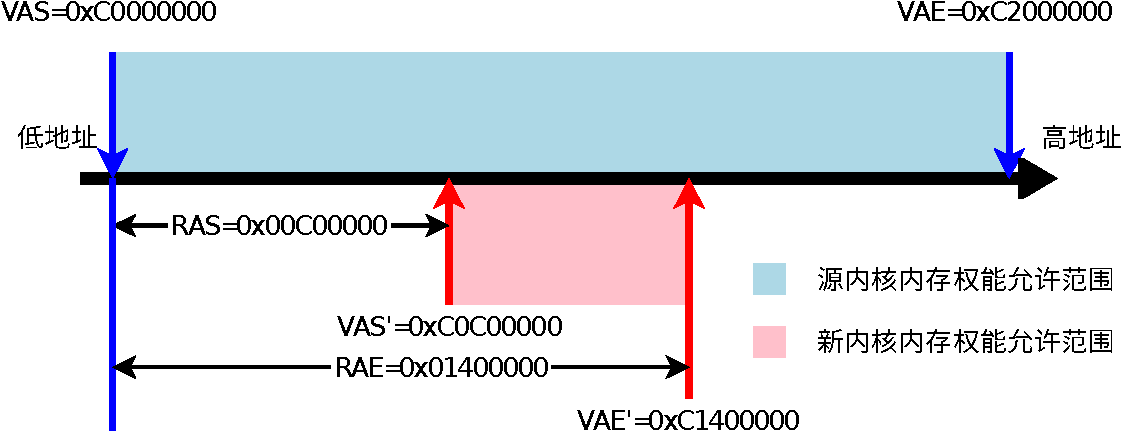
\includegraphics[width=0.72\textwidth]{Figure/image10.pdf}
    \caption{内核内存权能传递示例}
    \label{fig:3-3-kernel-memory-capability-transfer-example}
\end{figure}

此外，内核内存权能的上限值\footnote{也即内核结束绝对虚拟地址}不包括自身。在上例中，0xC1400000是不包括在新内核内存权能可操作的合法地址之内的，也即实际上允许的内核内存范围是0xC0C00000-0xC13FFFFF。上限必须大于下限，否则会返回错误。上限和下限在传入时都会被掩蔽后六位，对齐到64字节。如果内核内存登记表被配置为使用比64字节更大的槽位，那么内核会自动将传入的下限向上取整，上限向下取整，对齐到槽位大小。

本系统调用的可能返回值和一般的RME\_SVC\_CPT\_ADD操作完全一致，请参见\ref{subsec:2-transfer-a-capability}
。

\section{本章参考文献}\label{sec:3-chapter-bibliography}

\protect\phantomsection\label{cite:3-1}
{[}1{]}
Q. Wang, Y. Ren, M. Scaperoth, and G. Parmer, "Speck: A kernel for
scalable predictability," in Real-Time and Embedded Technology and
Applications Symposium (RTAS), 2015 IEEE, 2015, pp. 121-132.

\protect\phantomsection\label{cite:3-2}
{[}2{]} Emcraft Systems. uCLinux(2017).
\url{https://github.com/EmcraftSystems/linux-emcraft}

\protect\phantomsection\label{cite:3-3}
{[}3{]} G. Klein, K. Elphinstone, G. Heiser, J. Andronick, D. Cock, P.
Derrin, et al., "seL4: formal verification of an OS kernel," presented
at the Proceedings of the ACM SIGOPS 22nd symposium on Operating systems
principles, Big Sky, Montana, USA, 2009.

\protect\phantomsection\label{cite:3-4}
{[}4{]} Fiasco.OC website (2017).
\url{http://os.inf.tu-dresden.de/fiasco}


\chapter{进程和线程管理}\label{ch:process-and-thread-management}

\section{进程和线程概述}\label{sec:4-process-and-thread-overview}

进程（Process）和线程（Thread）是 RME 对其上执行的程序提供的基本抽象。RME 的进程和线程抽象层次较低，这与 Linux 等传统操作系统的高层次抽象实现是非常不同的。与传统操作系统相比，RME 的实现具备更高的灵活性和性能。

\subsection{进程概述}\label{subsec:4-process-overview}

在 RME 中，一个进程指的是拥有一个独立地址空间\footnote{也即一个独立页表}和一个权能表的最小保护域（Protection
Domain）。页表决定了进程的地址空间，权能表则决定了该进程中线程\footnote{或同步迁移调用，见第~\ref{subsec:5-async-communication-overview}~节}的权限。RME 不在内核态实现关于进程的其他所有信息；这些信息被全部留到用户态实现。

事实上，RME 中的进程与传统操作系统的进程相比几乎没有任何相似点，它们实际上是超轻量级的虚拟机，或者也可以被看作是容器（Container）。各个进程的权能表都有相互独立的权能号命名空间，没有系统全局的权能号。将多个进程合起来看成为一个相互隔离但又有一定联系的软件功能单元也是可以的。RME 进程在被用作轻量级虚拟机时，可以提供近乎于物理机的性能\hyperref[cite:4-4]{{[}4{]}}。

\subsection{线程概述}\label{subsec:4-thread-overview}

在 RME 中，一个线程指拥有一个独立指令流和一个栈的最小可调度实体。线程在 RME 中具有多个状态来标志其运行情况。本章所指的线程都是内核态线程，用户态线程由于与内核本身无关，因此不在此讨论。

\subsubsection{上下文的设计}\label{subsubsec:4-context-design}

在不同的系统中，线程的上下文（Context）主要有三种设计策略，分别如下：

\begin{enumerate}
\def\labelenumi{\arabic{enumi}.}
\item
  将线程的上下文放置在用户栈上。这是小型RTOS的常用策略。它足够灵活，完全不需要在内核中考虑线程上下文的存储，因而可以做的很紧凑，上下文的保存和恢复效率也很高。但这种设计无法被用于具备特权态的操作系统：内核态无法信任用户态提供的栈指针和缓冲区，在不做检查之前不能确保安全性，而若像 Linux 一样施加额外检查则会拖慢内核的执行效率。
\item
  将线程的上下文放置在内核栈上。这是 Linux 等宏内核的常用策略。这个方法的效率尚可，而且编程也很简单，但（1）每个线程在内核中都需要一个独立的内核栈，浪费内存空间，（2）在微内核中用权能的方法来管理栈这种用量动态变化的内核对象非常困难，（3）需要额外编写内核模式的上下文切换汇编函数。其中，（1）和（2）是致命的问题。
\item
  将线程的上下文放置在线程内核对象中。这是 RME 采取的策略：在切换上下文时，我们将暂存在内核栈上的上下文拷贝到当前线程的内核对象中，然后再将下一线程的内核对象中的上下文拷贝到内核栈上。当中断退出时，系统自然会切换到新的线程。采用这种设计会增加寄存器拷贝代码，且内核对象中需要一个独立的区域来保存寄存器上下文，但每个CPU仅需要准备一份固定的内核栈，非常适合资源吃紧的嵌入式系统，也有利于提高数据的局部性。当然，这种设计意味着内核本身不可能是可抢占（Preemptive）的；但是，无锁微内核本身短小精悍，其系统调用均拥有很小的WCET，不需要可抢占也可以达到比宏内核高的实时性。

  在协处理器存在时，此种设计的一个主要负面影响是线程内核对象的大小。协处理器（Coprocessor）或浮点处理器（Floating-Point
  Unit，FPU）通常具备一个很大的上下文，比如x86-64的AVX-512具备32个512位的寄存器，其最新的AMX矩阵运算扩展则甚至具备8KiB的矩阵寄存器。如果我们不加选择地为所有线程都配置如此大的协处理器上下文空间，则会造成巨大的内核内存浪费，因为不是每个线程都能用到它们。在那些异构CPU上\footnote{如各种 ARM 三丛集、x86-64 大小核等}，更是存在只有一部分CPU核支持高级协处理器的情况。为了避免浪费，在创建线程时可以指定一个上下文属性 Attr；它是一个位域，指示该线程需要启用哪些可选协处理器。在分配线程内核对象时，我们只分配启用的指令集的协处理器对应的上下文存储空间，而不为其它协处理器分配空间；在线程绑定到具体的CPU核时，我们会检查该核是否支持启用的协处理器，并在运行线程时关掉未启用的协处理器。当线程意外使用到未启用的协处理器时，将会产生未定义指令异常，用户态可以截获该异常，并分配上下文属性更强的新线程接替老线程的工作。

  对于如此巨大的寄存器上下文，高效地保存和恢复它们也需要技巧。即便线程声明了多种协处理器上下文，在实际运行中也未必会真正使用到它们。如果不加选择地对所有的上下文进行保存和恢复，就会导致不必要的切换延迟。因此，在实现协处理器上下文切换时，最好能够提前判断协处理器是否真正被使用，如果未被使用则可以不必保存和恢复它们的上下文。为了防止泄露协处理器信息，如果一个协处理器的状态从``使用中''变为``暂未使用''，需要清空协处理器的上下文。

  在实际使用中，推荐将需要高实时性的、不使用协处理器的线程在一组CPU上调度，将需要高算力的、使用协处理器的线程在另一组CPU上调度。这样，前者不仅不会受到后者巨大的上下文的干扰，也不会受到后者对CPU微架构造成的电流或功耗冲击\footnote{如启用 AVX-512 可能导致CPU大幅降频}的影响。

  对移植者而言，如果一个协处理器具备多个指令子集，是否要将它们分开成几种独立的上下文属性是可选的\footnote{如 SSE 包含 SSE、SSE2、SSE3、SSSE3 和 SSE4 等多个子集，是否要将它们独立为不同的属性是可选的}，但不推荐分得过细，因为 Attr 参数的位数有限；如果被分开成的指令子集之间有依赖关系，则内核必须在创建线程时检查这种依赖关系并在不满足时报告错误\footnote{如SSE3依赖于SSE2，则若某线程声明自己使用SSE3但不使用SSE2，内核必须报告该属性非法}；如果几个协处理器的寄存器有重叠部分，则内核必须使较大的协处理器声明自动隐含较小的协处理器声明\footnote{如 AVX-512 包含 AVX 和 SSE，则若某线程声明自己使用 AVX-512，则它不需要再声明自己使用 AVX 和 SSE}。
\end{enumerate}

\subsubsection{准虚拟化支持的设计}\label{subsubsec:4-paravirtualization-support-design}

微内核的一个很重要的用途是支持其它系统的准虚拟化：大名鼎鼎的 L4 就支持将 Linux 虚拟化后作为一组用户进程运行在 L4 上，称之为 L4Linux。要虚拟化其它操作系统，就需要正确模拟其内核态和用户态（对那些RTOS而言则是内核和用户程序）的交互，而其中最重要的交互是允许内核态修改用户态的线程的上下文。尽管 L4 等系统提供了系统调用来修改线程的上下文，但这终归需要经过微内核，相比于未虚拟化的原始系统还是慢了一步。

为了解决这个问题，RME 允许在创建线程时将线程指定为虚拟机专用型：它们绑定到CPU时需要指定一块微内核和用户态都能安全访问的内核内存，而后该线程的上下文将保存在那里\footnote{这种处理方式有些类似 VT-x 等硬件虚拟化技术提供的 VMCS 区域}；为了节约内存，该线程的内核对象就不再包括任何上下文信息。很明显，如果允许用户态指定任意的上下文保存地址，内核的完整性会遭到破坏。因此，指定的地址范围必须是内核编译时就配置好，而内核将通过某种手段\footnote{内核的页表映射代码或者受信任的用户态内存管理器}保证每个进程的该地址范围都映射有可读写的页面。在一切都静态分配的微控制器上，要保证这点就更加容易。

将虚拟机专用线程的上下文保存到用户态可能导致其上下文遭到任意修改。对于常规线程，用户态使用第~\ref{subsec:8-get-or-set-thread-register-set}~节所列的内核调用也能达成同样的目的。若线程的寄存器组含有和特权级转换或协处理器状态相关的寄存器\footnote{如 Cortex-M 的 LR 和 RISC-V 的 MSTATUS}，且内核在退出内核态、恢复寄存器时对这些寄存器的修改不加检查，将导致用户进程的提权或协处理器状态错乱。因此，每次在退出内核态时，都必须对用户态的关键寄存器进行检查，并修复错乱的值。

\subsubsection{调度器的设计}\label{subsubsec:4-scheduler-design}

在不同的系统中，调度器（Scheduler）主要有四种设计策略，分别如下：

\begin{enumerate}
\def\labelenumi{\arabic{enumi}.}
\item
  调度器完全在内核态。这一种实现之中，各个线程的时间片是完全自动填充的，并且调度策略的实现也完全处于内核态。采用此类实现的典型系统包括 Linux，全部的 L4 和 VxWorks。此类系统是非常传统的，在此不加叙述。
\item
  调度器完全在用户态，即便是优先级的判断和控制逻辑也在内核外部。当中断发生时，就切换到中断对应的线程进行中断处理；至于优先级和该执行哪个中断处理程序则完全由用户态调度器决定。这种实现具有极强的灵活性，并且可以很方便地实现空闲窃取调度（Slack
  Stealing
  Scheduling）。这是最原始的用户态调度设想，但是由于它引起了大量的线程切换，有过高的额外开销而没有使用价值。
\item
  抢占优先级在内核内部，包括就绪队列的其他部分在内核外部。当中断来临时，进行抢占并且立即运行中断处理线程。中断处理线程会启动中断后处理线程，然后在接收点上阻塞。如果在这个时间段内有其他的低优先级中断到来，那么低优先级中断会转化为送往对应调度器的调度器事件。高优先级的中断后处理线程完成中断处理后，调用调度器，处理在这段时间之内发生的所有调度器事件，并且决定下一个运行的线程。如果在这段时间之内，分配给后处理线程的时间片耗尽，那么我们切换到任意一个还有时间片的线程。它的坏处是，如果有一个低优先级的线程在高优先级线程执行时由于某中断而就绪，我们没办法在高优先级结束之后立即执行低优先级线程。我们必须先切换到用户态调度器，然后等待用户态调度器反复从系统中读取出全部的事件，并对这些事件的轻重缓急加以判断之后才能处理低优先级中断或者线程。这在某些场景下是不可忍受的。采用此类设计的典型系统为 Composite\hyperref[cite:4-1]{{[}1{]}}。值得一提的是，Composite 将优先级从标量（Scalar）扩展成了向量（Vector），各任务的优先级向量中的各标量分别对应于该任务在各子系统中的优先级，且只有当所有子系统都同意抢占时\footnote{抢占向量的每一个标量位都大于被抢占向量的每一个标量位}抢占才能发生\hyperref[cite:4-3]{{[}3{]}}，非常适合混合关键度系统中的串扰抑制。然而，由于每一次抢占都要进行向量比较，该优先级机制的执行时间虽然确定但过于缓慢，难以提供有意义的实时性；此外，存储向量形式的优先级也需要消耗大量内核内存，在微控制器中难以落地。在装备了加速器\footnote{GPU、NPU、ISP、DSP等}的系统中，每个任务在不同的加速器调度器上还可能有不同的优先级，只有当所有子系统的所有加速器都同意抢占时\footnote{抢占张量的每一个向量列都大于被抢占标量的每一个向量列}抢占才能发生；这样就势必要将优先级进一步扩展成张量（Tensor），优先级比较将变成难以想象的张量比较。
\item
  抢占优先级和运行队列在内核中，包括时间片管理等的其他部分在内核外。这是 RME 选择的解决方案：它更接近传统系统但又实现了用户态调度。好处是可以减小中断延迟，并且能够确保现在运行的线程总是就绪线程中优先级最高的。坏处则是每一次处理任何可能导致上下文切换的操作，都要处理内核的运行队列。因此，RME 的内核队列维护器采用了高效率设计以将这种影响降到最低。此外，内核仍然要给线程发送调度器事件来配合用户态调度。与Composite\hyperref[cite:4-1]{{[}1{]}}不同，RME 的优先级实现为一个标量。这使得系统的优先级必须被平铺（Flattened），不利于在内核中直接消除各个子系统之间的干扰，但可以大大加快调度原语的速度，从而方便在用户态实现适合混合关键度系统的向量或张量优先级调度算法。
\end{enumerate}

在 RME 中，每个线程都有一个抢占优先级，其数值越大，则优先级越高\footnote{这与某些系统是相反的；与常见的 FreeRTOS 则是一致的}。优先级的数量由宏 RME\_PREEMPT\_PRIO\_NUM 配置，系统中的优先级为从0到
RME\_PREEMPT\_PRIO\_NUM-1。其最高可以被配置为2的字长的一半次方。比如32位系统中，优先级的最大数量为2\textsuperscript{16}=65536。此外，每个线程在被创建时都会被指定一个优先级上限，一个线程不能通过系统调用创建拥有更高优先级上限的线程。在对一个线程做处理器绑定操作或优先级变更操作时，无法把被操作线程的优先级提高到其优先级上限以上。但是，一个拥有低优先级上限的线程可以把另一个线程的优先级提高到低优先级线程自身的优先级上限以上，只要被操作线程的优先级不被提高到超过被操作线程的优先级上限。优先级上限的实现参考了 seL4\hyperref[cite:4-2]{{[}2{]}}。

与其他也使用时间片传递的系统如 NOVA\hyperref[cite:4-5]{{[}5{]}}等不同，RME 的线程时间片不会在某个时点自动被系统填充，这也是 RME 的调度器在内核外的原因。如果一个线程的时间片耗尽，那么该线程将一直停止执行直到有其它线程向它转移时间片为止。

每个线程都具有一个用户决定的线程标识符（Thread
IDentifier，TID）。这个标识符是由用户在绑定（Bind）线程时决定的。在32位系统下，该标识符的范围为0-2\textsuperscript{16}-1；考虑到目前绝大多数32位设备现在都是嵌入式设备\footnote{基本上是微控制器或低端微处理器}，因此即便在某些状况下用户态需要全局唯一的TID，这个范围也是够用的。在64位系统下这个范围是0-2\textsuperscript{32}-1，在可预见的将来也是足够使用的。

此外，RME不在内核态实现诸如线程本地存储（Thread Local
Storage，TLS）等其他功能。这些功能会被用户态库实现。

\section{进程的操作}\label{sec:4-process-operations}

\subsection{进程的创建和删除}\label{subsec:4-process-creation-and-deletion}

要创建进程，需要一个权能表和一个可以作为顶层的页目录\footnote{也即顶层页目录权能，详见\ref{subsubsec:3-top-level-page-directory-flag}}。进程在 RME 中仅仅起到一个隔离保护域的作用；它没有独立的状态。销毁一个进程中所有的线程和同步迁移调用入口\footnote{详见第~\ref{subsec:5-sync-communication-overview}~节}并不会导致进程被销毁。

要删除进程，需要该进程中没有任何的线程存在，也没有任何的同步迁移调用入口\footnote{详见第~\ref{subsec:5-sync-communication-overview}~节}存在。只要通过进程权能指明要删除的进程就可以了。

\subsection{更改进程的权能表或页表}\label{subsec:4-change-process-capability-table-or-page-table}

进程的权能表和页表是可以在系统运行过程中动态更换的，并且动态更换总是立即生效。动态更换操作通常用来实现虚拟化功能中虚拟机或容器的切换，也可以用来实现快速跨进程通信等其他功能。

\section{线程的操作和状态}\label{sec:4-thread-operations-and-states}

\subsection{线程操作总览}\label{subsec:4-thread-operations-overview}

在 RME 中，线程是需要被绑定到某个CPU才能被操作的，而且只有它被绑定的那个CPU内核可以操作它。如果想要更改可以操作该线程的CPU，那么需要修改其绑定。在系统中线程有如下几个状态：

\begin{xltabular}{\textwidth}{@{}>{\hsize=0.5857\hsize\raggedright\arraybackslash}X>{\hsize=0.7809\hsize\raggedright\arraybackslash}X>{\hsize=1.6334\hsize\raggedright\arraybackslash}X@{}}
\caption{线程的状态}\label{tab:4-1-thread-states}\\
\toprule
状态 & 名称 & 说明\tabularnewline
\endfirsthead
\toprule
状态 & 名称 & 说明\tabularnewline
\midrule
\endhead
\bottomrule
\endlastfoot
就绪 & RME\_THD\_READY &
线程处于就绪态；其中当前CPU上优先级最高的一个被认为处于运行态。运行态在内核中不直接对应任何标志。\tabularnewline
超时 & RME\_THD\_TIMEOUT & 线程的时间片被用尽。\tabularnewline
阻塞 & RME\_THD\_BLOCKED & 线程被阻塞在某个接收点上。\tabularnewline
异常 & RME\_THD\_EXCPEND &
线程执行过程中发生了一个异常，被迫暂停。\tabularnewline
\end{xltabular}

这几个状态是可以互相转换的。当线程被创建时，它处于 RME\_THD\_TIMEOUT 状态，这表示它没有被绑定到某个CPU，也没有被分配时间片。接下来，我们将它绑定到某个核，此时它仍然处于 RME\_THD\_TIMEOUT 状态。然后设置它的入口和栈。最后，我们分配时间片给它。它会被放入内核就绪队列，进入RME\_THD\_READY状态；如果它是该CPU上优先级最高的线程，则它会抢占当前线程，并实际运行。

如果线程在执行过程中在某个接收点上被阻塞，线程会转换成 RME\_THD\_BLOCKED 状态。这种情况下，当阻塞被解除时线程会回到 RME\_THD\_READY 状态。

如果线程在执行过程中出现了异常，则它会转换到 RME\_THD\_EXCPEND 状态，并且向其父线程\footnote{调度器线程}发送一个调度器事件。如果线程在绑定时还指定了一个信号端点\footnote{详见第~\ref{subsec:5-async-communication-overview}~节}，那么该信号端点也会收到一个信号。要解除错误状态，需要重置其执行栈和入口，才能把线程置于 RME\_THD\_TIMEOUT 状态。

如果该线程在运行时用尽了自己的所有时间片，或者在时间片传递中将自己的时间片全部传递出去，或者在切换到其他线程时选择放弃当前所有时间片，那么它会进入 RME\_THD\_TIMEOUT 状态，并且向其父线程发送一个调度器事件。如果线程在绑定时还指定了一个信号端点，那么该信号端点也会收到一个信号。

当解除一个线程对某CPU的绑定时，该线程必须没有子线程。解除绑定时，对应于该线程的父线程调度器事件如果存在，那么也会被去掉。在 RME\_THD\_BLOCKED 下被解除绑定，那么当前阻塞会直接返回一个 RME\_ERR\_SIV\_FREE 的错误码\footnote{详见第~\ref{subsec:5-async-communication-overview}~节}。此外，在线程不是 RME\_THD\_EXCPEND 状态时，如果解除绑定，那么该线程的状态都将变成 RME\_THD\_TIMEOUT 状态。如果在 RME\_THD\_EXCPEND 状态下解除线程的绑定，那么线程将仍会维持在 RME\_THD\_EXCPEND 状态下。

\subsection{线程的创建和删除}\label{subsec:4-thread-creation-and-deletion}

当创建线程时，需要额外指明线程所在的进程、使用的协处理器，以及该线程是否是虚拟机专用线程。入口、栈等属性是通过其他内核调用设置的。

当线程被删除时，它必须被解除绑定。在删除线程时，我们会清空它的同步迁移调用栈\footnote{详见第~\ref{subsec:5-sync-communication-overview}~节}。

\subsection{把线程绑定到某CPU和解除绑定}\label{subsec:4-bind-thread-to-cpu-and-unbind}

创建线程后需要把它绑定到某个CPU才能够操作，而如果想要更换这种绑定，那么就需要先解除它对当前CPU的绑定。

绑定线程到某CPU需要指明线程的优先级，线程的父线程和一个TID。在哪个CPU上调用绑定函数，该线程即会被绑定到哪个CPU。绑定操作通过使用比较交换原子操作来进行，保证在多个CPU同时进行的操作中，只有一个会获得成功。另外还有一个信号端点作为可选参数，如果在绑定时指定了一个信号端点，那么该信号端点将接收到此线程的调度器信号。值得注意的是，TID并不需要是全局唯一的，用户态可以决定TID的分配策略。

解除绑定则仅仅需要指明需要解除绑定线程即可。当一个线程被解除了对某个CPU的绑定后，我们就可以把它绑定到其他的CPU了，也即实现了线程在不同处理器之间的迁移。这和那些线程在创建时就被永久绑定到某处理器的系统，如 Composite 等\hyperref[cite:4-1]{{[}1{]}}不同。

\subsection{设置线程的执行属性}\label{subsec:4-thread-execution-attributes}

在完成线程绑定后，我们需要设置线程的入口，堆栈和自定义参数。这三个值在会被传递给线程的寄存器组，在线程第一次运行时，用户态库根据前两个参数来找到用户态的线程入口和线程栈。需要注意的是，在区分虚拟地址和实地址的架构上，这两个值都是虚拟地址。

\subsection{线程分配时间片，修改优先级和运行}\label{subsec:4-thread-time-slice-allocation-priority-change-and-run}

在设置完现成的入口和栈之后，我们就可以给线程分配时间片，从而开始线程的运行了。RME 系统的时间片分配是由用户态调度器树组织的，而且每个CPU都有这样的一个调度器树，用来管理本CPU的运行时间分配。首先由系统的各CPU上的 Init 线程给用户态调度器分配时间片\footnote{Init线程的时间片为RME\_THD\_INIT\_TIME，是无限的}，然后再由这些用户态调度器按照它们各自的调度算法，把它们的时间片按照合适的比例传递给它们的各个子调度器，依此类推层层分配，从而完成线程的层次化调度。这种组织使得准虚拟化其他操作系统变得非常容易。各个CPU上的 Init 线程拥有无限的时间片，也即如果没有任何其他线程可以运行，我们总是去运行这个CPU上的 Init 线程\footnote{这也是为 Init 线程不允许阻塞在任何端点上的原因，详见第~\ref{sec:5-async-communication-operations}~节}。

在线程时间片分配完成后，线程即被放入每个核的就绪序列（Ready
Queue），并且会和当前运行的线程进行优先级比较。如果当前运行的线程的优先级较低，那么该线程会被立即投入运行。

我们可以修改一个已经被绑定到某个CPU的线程的优先级。在优先级修改后，如果该线程的优先级是最高的，而且它处于 RME\_THD\_READY 状态，那么它会被立即调度运行。

线程间传递时间片的做法借鉴了 Composite 的 TCap 机制，并且加以简化和改进\hyperref[cite:4-3]{{[}3{]}}。按持有时间片的多少和线程创建时间分类，在系统中有三种线程，分别如下表所示：

\begin{xltabular}{\textwidth}{@{}>{\hsize=0.7158\hsize\raggedright\arraybackslash}X>{\hsize=0.9241\hsize\raggedright\arraybackslash}X>{\hsize=1.3602\hsize\raggedright\arraybackslash}X@{}}
\caption{线程的分类}\label{tab:4-2-thread-categories}\\
\toprule
种类 & 创建时间 & 特点\tabularnewline
\endfirsthead
\toprule
种类 & 创建时间 & 特点\tabularnewline
\midrule
\endhead
\bottomrule
\endlastfoot
通常线程 & 在系统启动之后 &
时间片有限，并且持有总量不超过 RME\_THD\_INF\_TIME。\tabularnewline
无限线程 & 在系统启动之后 &
时间片无限，时间片持有量记做 RME\_THD\_INF\_TIME。\tabularnewline
初始线程 & 在系统启动之时 &
时间片无限，时间片持有量记做 RME\_THD\_INIT\_TIME。\tabularnewline
\end{xltabular}

几个宏的意义如下表所示：

\begin{xltabular}{\textwidth}{@{}>{\hsize=0.7708\hsize\raggedright\arraybackslash}X>{\hsize=1.2292\hsize\raggedright\arraybackslash}X@{}}
\caption{时间片宏定义的含义}\label{tab:4-3-time-slice-macro-definitions}\\
\toprule
宏名 & 意义\tabularnewline
\endfirsthead
\toprule
宏名 & 意义\tabularnewline
\midrule
\endhead
\bottomrule
\endlastfoot
RME\_THD\_INIT\_TIME &
为最大正整数数值，在32位系统下为0x7FFFFFFF。\tabularnewline
RME\_THD\_INF\_TIME & 为 RME\_THD\_INIT\_TIME-1，在 32 位系统下为 0x7FFFFFFE。\tabularnewline
\end{xltabular}

其中通常线程和无限时间片线程允许阻塞，也允许失去自己的所有时间片；初始线程则不允许这两点。在各个线程之间传递时间片有如下三种：

第一种是通常传递，这种传递会传递有限数量的时间片到其他线程；

第二种是无限传递，这种传递会传递无限数量的时间片到其他线程；

第三种是回收传递，这种传递会将源线程的时间片全部转移给目标线程，并且清零源线程的时间片。

值得注意的是，时间片传递是原子性的，也就是要么指定的量都被传递，要么就都不被传递，不可能发生部分传递的情况。三种传递的规则如下表所示。

\begin{xltabular}{\textwidth}{@{}>{\hsize=1.0000\hsize\raggedright\arraybackslash}X>{\hsize=1.0000\hsize\raggedright\arraybackslash}X>{\hsize=1.0000\hsize\raggedright\arraybackslash}X>{\hsize=1.0000\hsize\raggedright\arraybackslash}X>{\hsize=1.0000\hsize\raggedright\arraybackslash}X@{}}
\caption{时间片通常传递的规则}\label{tab:4-4-normal-time-transfer-rules}\\
\toprule
通常传递 & 源线程 & 初始线程 & 无限线程 & 通常线程\tabularnewline
\endfirsthead
\toprule
通常传递 & 源线程 & 初始线程 & 无限线程 & 通常线程\tabularnewline
\midrule
\endhead
\bottomrule
\endlastfoot
目标线程 & 初始线程 & -\/- & -\/- & T-\tabularnewline
& 无限线程 & -\/- & -\/- & T-\tabularnewline
& 通常线程 & -A & TA & TA\tabularnewline
\end{xltabular}

\begin{xltabular}{\textwidth}{@{}>{\hsize=1.0000\hsize\raggedright\arraybackslash}X>{\hsize=1.0000\hsize\raggedright\arraybackslash}X>{\hsize=1.0000\hsize\raggedright\arraybackslash}X>{\hsize=1.0000\hsize\raggedright\arraybackslash}X>{\hsize=1.0000\hsize\raggedright\arraybackslash}X@{}}
\caption{时间片无限传递的规则}\label{tab:4-5-infinite-time-transfer-rules}\\
\toprule
无限传递 & 源线程 & 初始线程 & 无限线程 & 通常线程\tabularnewline
\endfirsthead
\toprule
无限传递 & 源线程 & 初始线程 & 无限线程 & 通常线程\tabularnewline
\midrule
\endhead
\bottomrule
\endlastfoot
目标线程 & 初始线程 & -\/- & -\/- & S-\tabularnewline
& 无限线程 & -\/- & -\/- & S-\tabularnewline
& 通常线程 & -I & -I & TA\tabularnewline
\end{xltabular}

\begin{xltabular}{\textwidth}{@{}>{\hsize=1.0000\hsize\raggedright\arraybackslash}X>{\hsize=1.0000\hsize\raggedright\arraybackslash}X>{\hsize=1.0000\hsize\raggedright\arraybackslash}X>{\hsize=1.0000\hsize\raggedright\arraybackslash}X>{\hsize=1.0000\hsize\raggedright\arraybackslash}X@{}}
\caption{时间片回收传递的规则}\label{tab:4-6-reclaim-time-transfer-rules}\\
\toprule
回收传递 & 源线程 & 初始线程 & 无限线程 & 通常线程\tabularnewline
\endfirsthead
\toprule
回收传递 & 源线程 & 初始线程 & 无限线程 & 通常线程\tabularnewline
\midrule
\endhead
\bottomrule
\endlastfoot
目标线程 & 初始线程 & -\/- & S- & S-\tabularnewline
& 无限线程 & -\/- & S- & S-\tabularnewline
& 通常线程 & -I & SI & TA\tabularnewline
\end{xltabular}

表中：

``--''代表对源线程或目标线程没有影响；

``T''代表如果源线程的所有时间片都被转移出去，那么源线程会超时。

``S''代表源线程一定会超时。

``A''代表如果目标线程的时间片不溢出，那么会接受这些时间片。

``I''代表目标线程一定会变成无限线程。

\subsection{线程状态转移总览}\label{subsec:4-thread-state-transition-overview}

完善的线程状态转移图如下所示：

\begin{figure}[htbp]
    \centering
    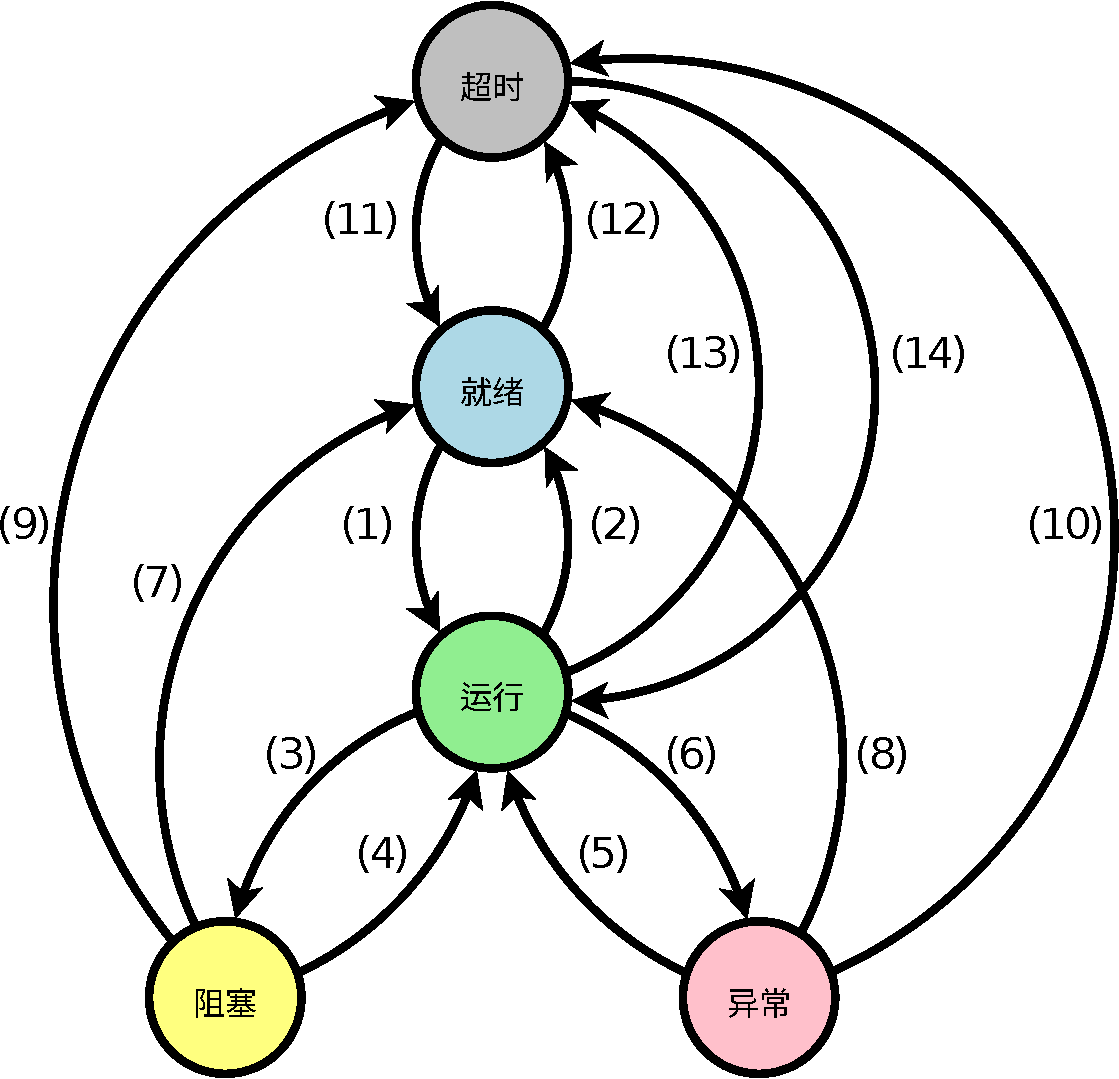
\includegraphics[width=0.72\textwidth]{Figure/image11.pdf}
    \caption{线程状态转移图}
    \label{fig:4-1-thread-state-transition-diagram}
\end{figure}

图中各个数字标号的意义如下所示：

\begin{xltabular}{\textwidth}{@{}>{\hsize=0.5279\hsize\raggedright\arraybackslash}X>{\hsize=1.4721\hsize\raggedright\arraybackslash}X@{}}
\caption{线程状态转移图中各标号的含义}\label{tab:4-7-thread-state-transition-labels}\\
\toprule
标号 & 代表意义\tabularnewline
\endfirsthead
\toprule
标号 & 代表意义\tabularnewline
\midrule
\endhead
\bottomrule
\endlastfoot
    (1) & 当前核上它是优先级最高的线程，因此由就绪态转入运行态。\tabularnewline
    (2) & 当前核上有更高优先级的线程打断了它的执行，因此由运行态转入就绪态。\tabularnewline
    (3) & 线程在一个信号端点处阻塞，因此由运行态转入阻塞态。\tabularnewline
    (4) & 线程收到了来自信号端点的信号，解除阻塞，而且是当前核上优先级最高的线程，并且其时间片没有耗尽，因此由阻塞态转入运行态。\tabularnewline
    (5) & 线程发生错误后藉由重新设置执行信息而恢复到可正常执行状态，而且是当前核上优先级最高的线程，并且其时间片没有耗尽，因此由异常态转入运行态。\tabularnewline
    (6) & 线程执行过程中发生了一个异常，因此从运行态转入异常态。\tabularnewline
    (7) & 线程收到了来自信号端点的信号，解除阻塞，并且其时间片没有耗尽，但它不是当前核上优先级最高的线程，因此由阻塞态转入就绪态。\tabularnewline
    (8) & 线程发生错误后藉由重新设置执行信息而恢复到可正常执行状态，并且其时间片没有耗尽，但它不是当前核上优先级最高的线程，因此由异常态转入就绪态。\tabularnewline
    (9) & 线程在等待信号端点时，被其他线程把自己的时间片传递出去，使得自己的时间片归零，因此在收到信号解除阻塞后由阻塞态转入超时态。\tabularnewline
    (10) & 线程发生错误后，被其他线程把自己的时间片传递出去，使得自己的时间片归零，因此在重新设置执行信息而恢复到可正常执行状态后由异常态转入超时态。\tabularnewline
    (11) & 线程被其他线程传递了时间片，重新进入可以运行的状态，但它不是当前核上优先级最高的线程，因此由超时态转入就绪态。\tabularnewline
    (12) & 线程在就绪状态时，被其他线程把自己的时间片传递出去，使得自己的时间片归零，因此由就绪态转入超时态。\tabularnewline
    (13) & 线程在运行过程中耗尽了自己的时间片，因此由运行态转入超时态。\tabularnewline
    (14) & 线程被其他线程传递了时间片，重新进入可以运行的状态，而且是当前核上优先级最高的线程，因此由超时态转入运行态。\tabularnewline
\end{xltabular}

其中，（6）（9）（10）（12）（13）等一切转入超时态和异常态的转换都会导致调度器事件的发送。

\section{进程功能列表}\label{sec:4-process-function-list}

与进程有关的内核功能如下：

\begin{xltabular}{\textwidth}{@{}>{\hsize=0.9445\hsize\raggedright\arraybackslash}X>{\hsize=0.7197\hsize\raggedright\arraybackslash}X>{\hsize=1.3358\hsize\raggedright\arraybackslash}X@{}}
\caption{进程相关内核功能}\label{tab:4-8-process-related-kernel-functions}\\
\toprule
调用号 & 类型 & 用途\tabularnewline
\endfirsthead
\toprule
调用号 & 类型 & 用途\tabularnewline
\midrule
\endhead
\bottomrule
\endlastfoot
RME\_SVC\_PRC\_CRT & 系统调用 & 创建进程\tabularnewline
RME\_SVC\_PRC\_DEL & 系统调用 & 删除进程\tabularnewline
RME\_SVC\_PRC\_CPT & 系统调用 & 替换进程的权能表\tabularnewline
RME\_SVC\_PRC\_PGT & 系统调用 &
替换进程的页表\footnote{顶层页目录}\tabularnewline
\end{xltabular}

进程权能的操作标志如下：

\begin{xltabular}{\textwidth}{@{}>{\hsize=0.9158\hsize\raggedright\arraybackslash}X>{\hsize=0.6763\hsize\raggedright\arraybackslash}X>{\hsize=1.4079\hsize\raggedright\arraybackslash}X@{}}
\caption{进程操作标志}\label{tab:4-9-process-operation-flags}\\
\toprule
标志 & 位 & 用途\tabularnewline
\endfirsthead
\toprule
标志 & 位 & 用途\tabularnewline
\midrule
\endhead
\bottomrule
\endlastfoot
RME\_PRC\_FLAG\_INV & {[}0{]} &
允许在该进程内创建同步迁移调用。\tabularnewline
RME\_PRC\_FLAG\_THD & {[}1{]} & 允许在该进程内创建线程。\tabularnewline
RME\_PRC\_FLAG\_CPT & {[}2{]} & 允许替换该进程的权能表。\tabularnewline
RME\_PRC\_FLAG\_PGT & {[}3{]} &
允许替换该进程的页表\footnote{顶层页目录}。\tabularnewline
\end{xltabular}

关于上表中的位{[}0{]}，请参见\ref{subsec:5-create-sync-invocation}
。

\subsection{创建进程}\label{subsec:4-create-a-process}

该操作会创建一个进程，并将其权能放入某个已存在的权能表。新创建的进程会引用权能表权能和页目录权能，一旦使用某对权能表/页目录权能创建了一个进程，那么这对权能在该进程被删除前就不能被移除/删除。进程权能没有单独分配的内核对象，因此不需要内核内存权能就能创建。

创建进程操作需要如下几个参数：

\begin{xltabular}{\textwidth}{@{}>{\hsize=0.7639\hsize\raggedright\arraybackslash}X>{\hsize=0.6758\hsize\raggedright\arraybackslash}X>{\hsize=0.6758\hsize\raggedright\arraybackslash}X>{\hsize=1.8846\hsize\raggedright\arraybackslash}X@{}}
\caption{创建进程的所需参数}\label{tab:4-10-create-process-parameters}\\
\toprule
参数名称 & 类型 & 域 & 描述\tabularnewline
\endfirsthead
\toprule
参数名称 & 类型 & 域 & 描述\tabularnewline
\midrule
\endhead
\bottomrule
\endlastfoot
Svc\_Num & ptr\_t & N & 必须为 RME\_SVC\_PRC\_CRT。\tabularnewline
Cap\_Cpt\_Crt & cid\_t & C &
一个对应于必须拥有 RME\_CPT\_FLAG\_CRT 属性的权能表权能的权能号，该权能号对应的权能指向要接受此新创建的进程权能的权能表。该权能号可以是一级或者二级查找编码。\tabularnewline
Cap\_Prc & cid\_t & P0 &
一个对应于接受该新创建的进程权能的权能表的某位置的权能号。该权能号对应的权能必须是空白的。该权能号只能是一级查找编码。\tabularnewline
Cap\_Cpt & cid\_t & P1 &
一个对应于必须拥有 RME\_CPT\_FLAG\_PRC\_CRT 属性的权能表权能的权能号，该权能号对应的权能指向要给新创建的进程使用的权能表。该权能号可以是一级或者二级查找编码。\tabularnewline
Cap\_Pgt & cid\_t & P2 &
一个对应于必须拥有 RME\_PGT\_FLAG\_PRC\_CRT 属性的页表权能的权能号，该权能号对应的权能指向要给新创建的进程使用的页表\footnote{顶层页目录}。该权能号可以是一级或者二级查找编码。\tabularnewline
Raw\_Pgt & ptr\_t & P2 &
一旦在移植时开启了用户态页表控制宏 RME\_PGT\_RAW\_USER，该参数即取代 Cap\_Pgt。它是处理器可直接识别的页表数据结构所在的物理地址，内核将直接使用它。因此，在使用用户态页表时，有进程创建权限的用户态进程必须可信。\tabularnewline
\end{xltabular}

该操作的返回值可能如下：

\begin{xltabular}{\textwidth}{@{}>{\hsize=0.8317\hsize\raggedright\arraybackslash}X>{\hsize=1.1683\hsize\raggedright\arraybackslash}X@{}}
\caption{创建进程的可能返回值}\label{tab:4-11-create-process-return-values}\\
\toprule
返回值 & 意义\tabularnewline
\endfirsthead
\toprule
返回值 & 意义\tabularnewline
\midrule
\endhead
\bottomrule
\endlastfoot
    0 & 操作成功。\tabularnewline
    RME\_ERR\_CPT\_RANGE & Cap\_Cpt\_Crt 的一级/二级查找超出了范围。\tabularnewline
    RME\_ERR\_CPT\_RANGE & Cap\_Cpt 的一级/二级查找超出了范围。\tabularnewline
    RME\_ERR\_CPT\_RANGE & Cap\_Pgt 的一级/二级查找超出了范围。\tabularnewline
    RME\_ERR\_CPT\_RANGE & Cap\_Prc 的一级查找超出了范围。\tabularnewline
    RME\_ERR\_CPT\_FROZEN & Cap\_Cpt\_Crt 的一级/二级查找的权能已经被冻结。\tabularnewline
    RME\_ERR\_CPT\_FROZEN & Cap\_Cpt 的一级/二级查找权能已经被冻结。\tabularnewline
    RME\_ERR\_CPT\_FROZEN & Cap\_Pgt 的一级/二级查找权能已经被冻结。\tabularnewline
    RME\_ERR\_CPT\_FROZEN & Cap\_Prc 被冻结，或者其它核正在该处创建权能。\tabularnewline
    RME\_ERR\_CPT\_TYPE & Cap\_Cpt\_Crt 或 Cap\_Cpt 不是权能表权能。\tabularnewline
    RME\_ERR\_CPT\_TYPE & Cap\_Pgt 不是页表权能。\tabularnewline
    RME\_ERR\_CPT\_FLAG & Cap\_Cpt\_Crt 无 RME\_CPT\_FLAG\_CRT 属性。\tabularnewline
    RME\_ERR\_CPT\_FLAG & Cap\_Cpt 无 RME\_CPT\_FLAG\_PRC\_CRT 属性。\tabularnewline
    RME\_ERR\_CPT\_FLAG & Cap\_Pgt 无 RME\_PGT\_FLAG\_PRC\_CRT 属性。\tabularnewline
    RME\_ERR\_CPT\_EXIST & Cap\_Prc 不是空白权能。\tabularnewline
\end{xltabular}

\subsection{删除进程}\label{subsec:4-delete-a-process}

该操作会删除一个进程。被删除的进程必须不含有线程或同步迁移调用（关于后者见同步通信机制）。删除进程需要以下几个参数：

\begin{xltabular}{\textwidth}{@{}>{\hsize=0.6910\hsize\raggedright\arraybackslash}X>{\hsize=0.6910\hsize\raggedright\arraybackslash}X>{\hsize=0.6910\hsize\raggedright\arraybackslash}X>{\hsize=1.9271\hsize\raggedright\arraybackslash}X@{}}
\caption{删除进程的所需参数}\label{tab:4-12-delete-process-parameters}\\
\toprule
参数名称 & 类型 & 域 & 描述\tabularnewline
\endfirsthead
\toprule
参数名称 & 类型 & 域 & 描述\tabularnewline
\midrule
\endhead
\bottomrule
\endlastfoot
Svc\_Num & ptr\_t & N & 必须为 RME\_SVC\_PRC\_DEL。\tabularnewline
Cap\_Cpt & cid\_t & C &
一个对应于必须拥有 RME\_CPT\_FLAG\_DEL 属性的权能表权能的权能号，该权能号对应的权能指向含有正被删除的进程权能的权能表。该权能号可以是一级或者二级查找编码。\tabularnewline
Cap\_Prc & cid\_t & P1 &
一个对应于将被删除的进程权能的权能号。该权能号对应的权能必须是一个进程权能。该权能号只能是一级查找编码。\tabularnewline
\end{xltabular}

该操作的返回值可能如下：

\begin{xltabular}{\textwidth}{@{}>{\hsize=0.6993\hsize\raggedright\arraybackslash}X>{\hsize=1.3007\hsize\raggedright\arraybackslash}X@{}}
\caption{删除进程的可能返回值}\label{tab:4-13-delete-process-return-values}\\
\toprule
返回值 & 意义\tabularnewline
\endfirsthead
\toprule
返回值 & 意义\tabularnewline
\midrule
\endhead
\bottomrule
\endlastfoot
    0 & 操作成功。\tabularnewline
    RME\_ERR\_CPT\_RANGE & Cap\_Cpt 的一级/二级查找超出了范围。\tabularnewline
    RME\_ERR\_CPT\_RANGE & Cap\_Prc 的一级查找超出了范围。\tabularnewline
    RME\_ERR\_CPT\_FROZEN & Cap\_Cpt 的一级/二级查找的权能已经被冻结。\tabularnewline
    RME\_ERR\_CPT\_FROZEN & Cap\_Prc 未被冻结。\tabularnewline
    RME\_ERR\_CPT\_TYPE & Cap\_Cpt 不是权能表权能。\tabularnewline
    RME\_ERR\_CPT\_TYPE & Cap\_Prc 不是进程权能。\tabularnewline
    RME\_ERR\_CPT\_NULL & Cap\_Prc 为空白权能。\tabularnewline
    RME\_ERR\_CPT\_NULL & 两个核同时试图删除该进程，此时未成功的核返回该值。\tabularnewline
    RME\_ERR\_CPT\_FLAG & Cap\_Cpt 无 RME\_CPT\_FLAG\_DEL 属性。\tabularnewline
    RME\_ERR\_CPT\_QUIE & Cap\_Prc 不安定。\tabularnewline
    RME\_ERR\_CPT\_REFCNT & Cap\_Prc 的引用计数不为 0，或者不为根权能\footnote{内部有线程或同步迁移调用}。\tabularnewline
\end{xltabular}

\needspace{30\baselineskip}
\subsection{更改进程的权能表}\label{subsec:4-change-process-capability-table}
\nopagebreak[4]

该操作会把进程的权能表替换成另外一个。替换完成后，立即生效。替换进程的权能表需要以下几个参数：

\begin{xltabular}{\textwidth}{@{}>{\hsize=0.6910\hsize\raggedright\arraybackslash}X>{\hsize=0.6910\hsize\raggedright\arraybackslash}X>{\hsize=0.6910\hsize\raggedright\arraybackslash}X>{\hsize=1.9271\hsize\raggedright\arraybackslash}X@{}}
\caption{更改进程权能表的所需参数}\label{tab:4-14-change-process-capability-table-parameters}\\
\toprule
参数名称 & 类型 & 域 & 描述\tabularnewline
\endfirsthead
\toprule
参数名称 & 类型 & 域 & 描述\tabularnewline
\midrule
\endhead
\bottomrule
\endlastfoot
Svc\_Num & ptr\_t & N & 必须为 RME\_SVC\_PRC\_CPT。\tabularnewline
Cap\_Prc & cid\_t & P1 &
一个对应于必须拥有 RME\_PRC\_FLAG\_CPT 属性的进程权能的权能号，该权能号对应的权能指向要修改权能表的进程。该权能号可以是一级或者二级查找编码。\tabularnewline
Cap\_Cpt & cid\_t & P2 &
一个对应于必须拥有 RME\_CPT\_FLAG\_PRC\_CPT 属性的权能表权能的权能号，该权能号对应的权能指向要给进程使用的权能表。该权能号可以是一级或者二级查找编码。\tabularnewline
\end{xltabular}

该操作的返回值可能如下：

\begin{xltabular}{\textwidth}{@{}>{\hsize=0.7784\hsize\raggedright\arraybackslash}X>{\hsize=1.2216\hsize\raggedright\arraybackslash}X@{}}
\caption{更改进程权能表的所需返回值}\label{tab:4-15-change-process-capability-table-return-values}\\
\toprule
返回值 & 意义\tabularnewline
\endfirsthead
\toprule
返回值 & 意义\tabularnewline
\midrule
\endhead
\bottomrule
\endlastfoot
    0 & 操作成功。\tabularnewline
    RME\_ERR\_CPT\_RANGE & Cap\_Prc 的一级/二级查找超出了范围。\tabularnewline
    RME\_ERR\_CPT\_RANGE & Cap\_Cpt 的一级查找超出了范围。\tabularnewline
    RME\_ERR\_CPT\_FROZEN & Cap\_Prc 的一级/二级查找的权能已经被冻结。\tabularnewline
    RME\_ERR\_CPT\_FROZEN & Cap\_Cpt 的一级/二级查找的权能已经被冻结。\tabularnewline
    RME\_ERR\_CPT\_TYPE & Cap\_Prc 不是进程权能。\tabularnewline
    RME\_ERR\_CPT\_TYPE & Cap\_Cpt 不是权能表权能。\tabularnewline
    RME\_ERR\_CPT\_NULL & Cap\_Prc 或 Cap\_Cpt 为空白权能。\tabularnewline
    RME\_ERR\_CPT\_FLAG & Cap\_Prc 无 RME\_PRC\_FLAG\_CPT 属性。\tabularnewline
    RME\_ERR\_CPT\_FLAG & Cap\_Cpt 无 RME\_CPT\_FLAG\_PRC\_CPT 属性。\tabularnewline
    RME\_ERR\_PTH\_CONFLICT & 两个核同时试图替换权能表，此时未成功的核返回该值。\tabularnewline
\end{xltabular}

\subsection{更改进程的页表}\label{subsec:4-change-process-page-table}

该操作会把进程的页表替换成另外一个。替换完成后，立即生效。替换进程的页表需要以下几个参数：

\begin{xltabular}{\textwidth}{@{}>{\hsize=0.6910\hsize\raggedright\arraybackslash}X>{\hsize=0.6910\hsize\raggedright\arraybackslash}X>{\hsize=0.6910\hsize\raggedright\arraybackslash}X>{\hsize=1.9271\hsize\raggedright\arraybackslash}X@{}}
\caption{更改进程页表的所需参数}\label{tab:4-16-change-process-page-table-parameters}\\
\toprule
参数名称 & 类型 & 域 & 描述\tabularnewline
\endfirsthead
\toprule
参数名称 & 类型 & 域 & 描述\tabularnewline
\midrule
\endhead
\bottomrule
\endlastfoot
Svc\_Num & ptr\_t & N & 必须为 RME\_SVC\_PRC\_PGT。\tabularnewline
Cap\_Prc & cid\_t & P1 &
一个对应于必须拥有 RME\_PRC\_FLAG\_PGT 属性的进程权能的权能号，该权能号对应的权能指向要修改页表\footnote{顶层页目录}的进程。该权能号可以是一级或者二级查找编码。\tabularnewline
Cap\_Pgt & cid\_t & P2 &
一个对应于必须拥有 RME\_PGT\_FLAG\_PRC\_PGT 属性的页目录权能的权能号，该权能号对应的权能指向要给进程使用的页表\footnote{顶层页目录}。该权能号可以是一级或者二级查找编码。\tabularnewline
Raw\_Pgt & ptr\_t & P2 &
一旦在移植时开启了用户态页表控制宏RME\_PGT\_RAW\_USER，该参数即取代Cap\_Pgt。它是处理器可直接识别的页表数据结构所在的物理地址，内核将直接使用它。因此，在使用用户态页表时，有本权限的用户态进程必须可信。\tabularnewline
\end{xltabular}

该操作的返回值可能如下：

\begin{xltabular}{\textwidth}{@{}>{\hsize=0.7880\hsize\raggedright\arraybackslash}X>{\hsize=1.2120\hsize\raggedright\arraybackslash}X@{}}
\caption{更改进程页表的可能返回值}\label{tab:4-17-change-process-page-table-return-values}\\
\toprule
返回值 & 意义\tabularnewline
\endfirsthead
\toprule
返回值 & 意义\tabularnewline
\midrule
\endhead
\bottomrule
\endlastfoot
    0 & 操作成功。\tabularnewline
    RME\_ERR\_CPT\_RANGE & Cap\_Prc 的一级/二级查找超出了范围。\tabularnewline
    RME\_ERR\_CPT\_RANGE & Cap\_Pgt 的一级查找超出了范围。\tabularnewline
    RME\_ERR\_CPT\_FROZEN & Cap\_Prc 的一级/二级查找的权能已经被冻结。\tabularnewline
    RME\_ERR\_CPT\_FROZEN & Cap\_Pgt 的一级/二级查找的权能已经被冻结。\tabularnewline
    RME\_ERR\_CPT\_TYPE & Cap\_Prc 不是进程权能。\tabularnewline
    RME\_ERR\_CPT\_TYPE & Cap\_Pgt 不是页表权能。\tabularnewline
    RME\_ERR\_CPT\_NULL & Cap\_Prc 或 Cap\_Pgt 为空白权能。\tabularnewline
    RME\_ERR\_CPT\_FLAG & Cap\_Prc 无 RME\_PRC\_FLAG\_PGT 属性。\tabularnewline
    RME\_ERR\_CPT\_FLAG & Cap\_Pgt 无 RME\_PGT\_FLAG\_PRC\_PGT 属性。\tabularnewline
    RME\_ERR\_PTH\_CONFLICT & 两个核同时试图替换页表，此时未成功的核返回该值。\tabularnewline
\end{xltabular}

\section{线程功能列表}\label{sec:4-thread-function-list}

与线程有关的内核功能如下：

\begin{xltabular}{\textwidth}{@{}>{\hsize=1.0550\hsize\raggedright\arraybackslash}X>{\hsize=0.6673\hsize\raggedright\arraybackslash}X>{\hsize=1.2777\hsize\raggedright\arraybackslash}X@{}}
\caption{线程相关内核功能}\label{tab:4-18-thread-related-kernel-functions}\\
\toprule
调用号 & 类型 & 用途\tabularnewline
\endfirsthead
\toprule
调用号 & 类型 & 用途\tabularnewline
\midrule
\endhead
\bottomrule
\endlastfoot
RME\_SVC\_THD\_CRT & 系统调用 & 创建线程\tabularnewline
RME\_SVC\_THD\_DEL & 系统调用 & 删除线程\tabularnewline
RME\_SVC\_THD\_SCHED\_BIND & 系统调用 & 将线程绑定到某CPU\tabularnewline
RME\_SVC\_THD\_SCHED\_FREE & 系统调用 &
将线程从某CPU上释放\footnote{顶层页目录}\tabularnewline
RME\_SVC\_THD\_EXEC\_SET & 系统调用 &
设置线程的执行属性\footnote{入口和栈}\tabularnewline
RME\_SVC\_THD\_SCHED\_PRIO & 系统调用 & 更改线程的优先级\tabularnewline
RME\_SVC\_THD\_SCHED\_RCV & 系统调用 &
收取线程的调度器事件\tabularnewline
RME\_SVC\_THD\_TIME\_XFER & 系统调用 & 在线程间传递时间片\tabularnewline
RME\_SVC\_THD\_SWT & 系统调用 & 切换到某同优先级线程\tabularnewline
\end{xltabular}

线程权能的操作标志如下：

\begin{xltabular}{\textwidth}{@{}>{\hsize=1.2600\hsize\raggedright\arraybackslash}X>{\hsize=0.5400\hsize\raggedright\arraybackslash}X>{\hsize=1.2000\hsize\raggedright\arraybackslash}X@{}}
\caption{线程操作标志}\label{tab:4-19-thread-operation-flags}\\
\toprule
标志 & 位 & 用途\tabularnewline
\endfirsthead
\toprule
标志 & 位 & 用途\tabularnewline
\midrule
\endhead
\bottomrule
\endlastfoot
RME\_THD\_FLAG\_EXEC\_SET & {[}0{]} &
允许设置该线程的执行属性。\tabularnewline
RME\_THD\_FLAG\_SCHED\_CHILD & {[}1{]} &
允许在该线程在绑定操作中作为子线程。\tabularnewline
RME\_THD\_FLAG\_SCHED\_PARENT & {[}2{]} &
允许在该线程在绑定操作中作为父线程。\tabularnewline
RME\_THD\_FLAG\_SCHED\_PRIO & {[}3{]} &
允许更改该线程的优先级。\tabularnewline
RME\_THD\_FLAG\_SCHED\_FREE & {[}4{]} &
允许解除该线程对某CPU的绑定。\tabularnewline
RME\_THD\_FLAG\_SCHED\_RCV & {[}5{]} &
允许收取该线程的调度器事件。\tabularnewline
RME\_THD\_FLAG\_XFER\_SRC & {[}6{]} &
允许该线程在时间传递中作为源。\tabularnewline
RME\_THD\_FLAG\_XFER\_DST & {[}7{]} &
允许该线程在时间传递中作为目标。\tabularnewline
RME\_THD\_FLAG\_SWT & {[}8{]} &
允许切换操作切换到该线程。\tabularnewline
\end{xltabular}

\subsection{创建线程}\label{subsec:4-create-a-thread}

该操作会创建一个线程，并将其权能放入某个已存在的权能表。新创建的线程是没有绑定到任何CPU，没有TID，并处于 RME\_THD\_TIMEOUT 状态的。为了防止一个线程新建超过自身优先级上限的线程而破坏子系统之间的隔离，任何线程都无法创建高于自身优先级上限的线程。

线程会引用创建时指定的进程，一旦使用在某进程内创建了一个线程，那么这个进程在该线程被删除前就不能被删除。考虑到部分架构中向量寄存器数量较多，本操作允许指定一个上下文属性，说明该线程允许启用的指令集，以节约内核内存的使用。本操作还允许线程映射其寄存器组到用户态；如果指定映射到用户态，则运行在用户态的虚拟机监视器可以随时修改其上下文，从而大大方便虚拟化相关功能的编程。如果内核在配置时就决定不使用虚拟化映射功能\footnote{详见第~\ref{subsec:7-general-macro-definitions}~节}，则该功能不能使用。创建线程操作需要如下几个参数：

\begin{xltabular}{\textwidth}{@{}>{\hsize=0.6786\hsize\raggedright\arraybackslash}X>{\hsize=0.6786\hsize\raggedright\arraybackslash}X>{\hsize=0.7502\hsize\raggedright\arraybackslash}X>{\hsize=1.8926\hsize\raggedright\arraybackslash}X@{}}
\caption{创建线程的所需参数}\label{tab:4-20-create-thread-parameters}\\
\toprule
参数名称 & 类型 & 域 & 描述\tabularnewline
\endfirsthead
\toprule
参数名称 & 类型 & 域 & 描述\tabularnewline
\midrule
\endhead
\bottomrule
\endlastfoot
Svc\_Num & ptr\_t & N{[}5:0{]} & 必须为 RME\_SVC\_THD\_CRT。\tabularnewline
Cap\_Cpt & cid\_t & C &
一个对应于必须拥有 RME\_CPT\_FLAG\_CRT 属性的权能表权能的权能号，该权能号对应的权能指向要接受此新创建的线程权能的权能表。该权能号可以是一级或者二级查找编码。\tabularnewline
Cap\_Kom & cid\_t & P1.D1 &
一个内核内存权能号，其标识的内核内存范围必须能够放下线程内核对象，并且要拥有 RME\_KOM\_FLAG\_THD 属性。该权能号可以是一级或二级查找编码。\tabularnewline
Cap\_Thd & cid\_t & P1.D0 &
一个对应于接受该新创建的线程权能的权能表的某位置的权能号。该权能号对应的权能必须是空白的。该权能号只能是一级查找编码。\tabularnewline
Cap\_Prc & cid\_t & P2.D1 &
一个对应于必须拥有 RME\_PRC\_FLAG\_THD 属性的进程权能的权能号，该权能号对应的权能指向包含新创建的线程的进程。该权能号可以是一级或者二级查找编码。\tabularnewline
Max\_Prio & ptr\_t & P2.D0 & 该线程的优先级上限。\tabularnewline
Raddr & ptr\_t & P3 &
新创建的线程内核对象要使用的内核起始相对虚拟地址。这个地址是相对于Cap\_Kom对应的内核权能的起始虚拟地址的。\tabularnewline
Attr & ptr\_t & N{[}X/2-1:7{]} &
指定线程的扩展指令集上下文属性。对于不同的架构，这个参数的意义不同，但在所有的架构中0都代表不进行任何指令集扩展，不分配、保存和恢复任何协处理器的寄存器状态。对于32位处理器，这个参数有9位，对于64位处理器，这个参数有25位。\tabularnewline
Is\_Hyp & ptr\_t & N{[}6{]} &
如果设置为0，系统会在内核中分配保存线程上下文的空间，这是通常情况。如果不为0，则线程将映射其寄存器到用户态，此时需要在绑定线程到CPU时设置映射的具体地址。\tabularnewline
\end{xltabular}

该操作的返回值可能如下：

\begin{xltabular}{\textwidth}{@{}>{\hsize=0.6791\hsize\raggedright\arraybackslash}X>{\hsize=1.3209\hsize\raggedright\arraybackslash}X@{}}
\caption{创建线程的可能返回值}\label{tab:4-21-create-thread-return-values}\\
\toprule
返回值 & 意义\tabularnewline
\endfirsthead
\toprule
返回值 & 意义\tabularnewline
\midrule
\endhead
\bottomrule
\endlastfoot
    0 & 操作成功。\tabularnewline
    RME\_ERR\_CPT\_RANGE & Cap\_Cpt 的一级/二级查找超出了范围。\tabularnewline
    RME\_ERR\_CPT\_RANGE & Cap\_Kom 的一级/二级查找超出了范围。\tabularnewline
    RME\_ERR\_CPT\_RANGE & Cap\_Prc 的一级/二级查找超出了范围。\tabularnewline
    RME\_ERR\_CPT\_RANGE & Cap\_Thd 的一级查找超出了范围。\tabularnewline
    RME\_ERR\_CPT\_FROZEN & Cap\_Cpt 的一级/二级查找的权能已经被冻结。\tabularnewline
    RME\_ERR\_CPT\_FROZEN & Cap\_Kom 的一级/二级查找的权能已经被冻结。\tabularnewline
    RME\_ERR\_CPT\_FROZEN & Cap\_Prc 的一级/二级查找权能已经被冻结。\tabularnewline
    RME\_ERR\_CPT\_FROZEN & Cap\_Thd 被冻结，或者其它核正在该处创建权能。\tabularnewline
    RME\_ERR\_CPT\_TYPE & Cap\_Cpt 不是权能表权能。\tabularnewline
    RME\_ERR\_CPT\_TYPE & Cap\_Kom 不是内核内存权能。\tabularnewline
    RME\_ERR\_CPT\_TYPE & Cap\_Prc 不是进程权能。\tabularnewline
    RME\_ERR\_CPT\_FLAG & Cap\_Cpt 无 RME\_CPT\_FLAG\_CRT 属性。\tabularnewline
    RME\_ERR\_CPT\_FLAG & Cap\_Kom 无 RME\_KOM\_FLAG\_THD 属性，或范围错误。\tabularnewline
    RME\_ERR\_CPT\_FLAG & Cap\_Prc 无 RME\_PRC\_FLAG\_THD 属性。\tabularnewline
    RME\_ERR\_CPT\_EXIST & Cap\_Thd 不是空白权能。\tabularnewline
    RME\_ERR\_CPT\_KOT & 分配内核内存失败。\tabularnewline
    RME\_ERR\_PTH\_PRIO & 试图创建比自身拥有更高的优先级上限的线程，或者传入的优先级上限过大，超过了系统配置时允许的上限。\tabularnewline
\bottomrule
\end{xltabular}

\needspace{30\baselineskip}
\subsection{删除线程}\label{subsec:4-delete-a-thread}
\nopagebreak[4]

该操作会删除一个线程。被删除的线程必须已经被解除绑定。删除线程需要以下几个参数：

\begin{xltabular}{\textwidth}{@{}>{\hsize=0.6910\hsize\raggedright\arraybackslash}X>{\hsize=0.6910\hsize\raggedright\arraybackslash}X>{\hsize=0.6910\hsize\raggedright\arraybackslash}X>{\hsize=1.9271\hsize\raggedright\arraybackslash}X@{}}
\caption{删除线程的所需参数}\label{tab:4-22-delete-thread-parameters}\\
\toprule
参数名称 & 类型 & 域 & 描述\tabularnewline
\endfirsthead
\toprule
参数名称 & 类型 & 域 & 描述\tabularnewline
\midrule
\endhead
Svc\_Num & ptr\_t & N & 必须为 RME\_SVC\_THD\_DEL。\tabularnewline
Cap\_Cpt & cid\_t & C &
一个对应于必须拥有 RME\_CPT\_FLAG\_DEL 属性的权能表权能的权能号，该权能号对应的权能指向含有正被删除的线程权能的权能表。该权能号可以是一级或者二级查找编码。\tabularnewline
Cap\_Thd & cid\_t & P1 &
一个对应于将被删除的线程权能的权能号。该权能号对应的权能必须是一个线程权能。该权能号只能是一级查找编码。\tabularnewline
\end{xltabular}

该操作的返回值可能如下：

\begin{xltabular}{\textwidth}{@{}>{\hsize=0.7784\hsize\raggedright\arraybackslash}X>{\hsize=1.2216\hsize\raggedright\arraybackslash}X@{}}
\caption{删除线程的可能返回值}\label{tab:4-23-delete-thread-return-values}\\
\toprule
返回值 & 意义\tabularnewline
\endfirsthead
\toprule
返回值 & 意义\tabularnewline
\midrule
\endhead
\bottomrule
\endlastfoot
    0 & 操作成功。\tabularnewline
    RME\_ERR\_CPT\_RANGE & Cap\_Cpt 的一级/二级查找超出了范围。\tabularnewline
    RME\_ERR\_CPT\_RANGE & Cap\_Thd 的一级查找超出了范围。\tabularnewline
    RME\_ERR\_CPT\_FROZEN & Cap\_Cpt 的一级/二级查找的权能已经被冻结。\tabularnewline
    RME\_ERR\_CPT\_FROZEN & Cap\_Thd 未被冻结。\tabularnewline
    RME\_ERR\_CPT\_TYPE & Cap\_Cpt 不是权能表权能。\tabularnewline
    RME\_ERR\_CPT\_TYPE & Cap\_Thd 不是线程权能。\tabularnewline
    RME\_ERR\_CPT\_NULL & Cap\_Thd 为空白权能。\tabularnewline
    RME\_ERR\_CPT\_NULL & 两个核同时试图删除该线程，此时未成功的核返回该值。\tabularnewline
    RME\_ERR\_CPT\_FLAG & Cap\_Cpt 无 RME\_CPT\_FLAG\_DEL 属性。\tabularnewline
    RME\_ERR\_CPT\_QUIE & Cap\_Thd 不安定。\tabularnewline
    RME\_ERR\_CPT\_REFCNT & Cap\_Thd 的引用计数不为 0，或者不为根权能。\tabularnewline
    RME\_ERR\_PTH\_INVSTATE & 该线程仍然处于被绑定状态。\tabularnewline
\end{xltabular}

\subsection{将线程绑定到某CPU}\label{subsec:4-bind-a-thread-to-a-cpu}

该操作会将线程绑定到某CPU上。被设置的线程必须未被绑定于任何CPU。在哪个CPU上调用本函数，绑定就完成在哪个CPU上。对于那些希望将寄存器上下文映射到用户态以方便修改的线程，该操作还会设置上下文的映射地址：对这段地址的管理由用户态下的受信任守护进程全权负责，内核在启动时只保证这个地址既可以由内核态访问，也可以由用户态访问，且不会导致缺页中断。将线程绑定到某CPU需要以下几个参数：

\begin{xltabular}{\textwidth}{@{}>{\hsize=0.8146\hsize\raggedright\arraybackslash}X>{\hsize=0.6652\hsize\raggedright\arraybackslash}X>{\hsize=0.6652\hsize\raggedright\arraybackslash}X>{\hsize=1.8550\hsize\raggedright\arraybackslash}X@{}}
\caption{将线程绑定到某CPU的所需参数}\label{tab:4-24-bind-thread-to-cpu-parameters}\\
\toprule
参数名称 & 类型 & 域 & 描述\tabularnewline
\endfirsthead
\toprule
参数名称 & 类型 & 域 & 描述\tabularnewline
\midrule
\endhead
\bottomrule
\endlastfoot
Svc\_Num & ptr\_t & N & 必须为 RME\_SVC\_THD\_SCHED\_BIND。\tabularnewline
Cap\_Thd & cid\_t & C &
一个对应于必须拥有 RME\_THD\_FLAG\_SCHED\_CHILD 属性的线程权能的权能号，该权能号对应的权能指向被绑定的线程。该权能号可以是一级或者二级查找编码。\tabularnewline
Cap\_Thd\_Sched & cid\_t & P1.D1 &
一个对应于必须拥有 RME\_THD\_FLAG\_SCHED\_PARENT 属性的线程权能的权能号，该权能号对应的权能指向被绑定的线程的父线程。该父线程必须已经被绑定于调用本函数的CPU。该权能号可以是一级或者二级查找编码。\tabularnewline
Cap\_Sig & cid\_t & P1.D0 &
一个对应于必须拥有 RME\_SIG\_FLAG\_SCHED 属性的信号端点权能的权能号。当调度器事件发生\footnote{线程超时或错误，其中超时可能由线程在运行时消耗所有时间片或者其时间片完全被传递给其他线程所致}时，该端点会收到一个信号。该权能号可以是一级或者二级查找编码，而且也是可选的。如果不希望接收调度器信号，则可以传入 RME\_CID\_NULL\footnote{一个半字长 INT\_MIN（负值），在 32 位系统上为 0x8000，在 64 位系统上为 0x80000000}。\tabularnewline
TID & tid\_t & P2.D1 &
用户提供的TID。RME 本身并不检查系统中是否有两个线程拥有相同的ID；至于是否要做这种检查是用户态的事情。\tabularnewline
Prio & ptr\_t & P2.D0 &
被绑定的线程的抢占优先级。在 RME 中线程的优先级从0开始计算，值越大优先级越高。这个值不能超过该线程固有的优先级上限。\tabularnewline
Haddr & ptr\_t & P3 &
用户态寄存器上下文的映射地址。这个地址必须位于系统中专门用于线程上下文映射的地址范围，也即大于或等于基地址RME\_HYP\_VA\_BASE，小于结束地址RME\_HYP\_VA\_BASE+
RME\_HYP\_SIZE，而且要对齐到字。对于常规的线程，设置为NULL即可。\tabularnewline
\end{xltabular}

该操作的返回值可能如下：

\begin{xltabular}{\textwidth}{@{}>{\hsize=0.7880\hsize\raggedright\arraybackslash}X>{\hsize=1.2120\hsize\raggedright\arraybackslash}X@{}}
\caption{将线程绑定到某CPU的可能返回值}\label{tab:4-25-bind-thread-to-cpu-return-values}\\
\toprule
返回值 & 意义\tabularnewline
\endfirsthead
\toprule
返回值 & 意义\tabularnewline
\midrule
\endhead
\bottomrule
\endlastfoot
    0 & 操作成功。\tabularnewline
    RME\_ERR\_CPT\_RANGE & Cap\_Thd 或 Cap\_Thd\_Sched 的一级/二级查找超出了范围。\tabularnewline
    RME\_ERR\_CPT\_FROZEN & Cap\_Thd 或 Cap\_Thd\_Sched 的一级/二级查找的权能已经被冻结。\tabularnewline
    RME\_ERR\_CPT\_TYPE & Cap\_Thd 或 Cap\_Thd\_Sched 不是线程权能，或者为空白权能。\tabularnewline
    RME\_ERR\_CPT\_FLAG & Cap\_Thd 无 RME\_THD\_FLAG\_SCHED\_CHILD 属性。\tabularnewline
    RME\_ERR\_CPT\_FLAG & Cap\_Thd\_Sched 无 RME\_THD\_FLAG\_SCHED\_PARENT 属性。\tabularnewline
    RME\_ERR\_CPT\_FLAG & 当传入 Cap\_Sig 时，它没有 RME\_SIG\_FLAG\_SCHED 属性。\tabularnewline
    RME\_ERR\_CPT\_FLAG & 欲绑定的处理器不支持该线程创建时登记的 Attr。\tabularnewline
    RME\_ERR\_PTH\_HADDR & 传入的Haddr不在系统允许范围内，不合法。\tabularnewline
    RME\_ERR\_PTH\_NOTIF & 试图注册自己为自己的父线程，不合法。\tabularnewline
    RME\_ERR\_PTH\_PRIO & 抢占优先级超过了该线程固有的优先级上限，不合法。\tabularnewline
    RME\_ERR\_PTH\_INVSTATE & Cap\_Thd 处于被绑定状态或 Cap\_Thd\_Sched 处于未被绑定状态。\tabularnewline
    RME\_ERR\_PTH\_INVSTATE & Cap\_Thd\_Sched 被绑定到了和调用本函数的 CPU 不同的 CPU。\tabularnewline
    RME\_ERR\_PTH\_CONFLICT & 如果两个CPU同时尝试绑定，在失败的CPU上返回该值。\tabularnewline
\end{xltabular}

\subsection{解除线程对某CPU的绑定}\label{subsec:4-unbind-a-thread-from-a-cpu}

该操作会解除线程对某个CPU的绑定。被解除绑定的线程自身不能有子线程。如果被解除绑定的线程向其父线程发送了调度器事件，那么这个事件会被撤销。如果被解除绑定的线程阻塞，那么它同时会让这次阻塞接收强制结束并返回RME\_ERR\_SIV\_FREE。解除线程对某CPU的绑定需要以下几个参数：

\begin{xltabular}{\textwidth}{@{}>{\hsize=0.6910\hsize\raggedright\arraybackslash}X>{\hsize=0.6910\hsize\raggedright\arraybackslash}X>{\hsize=0.6910\hsize\raggedright\arraybackslash}X>{\hsize=1.9271\hsize\raggedright\arraybackslash}X@{}}
\caption{解除线程对某CPU绑定的所需参数}\label{tab:4-26-unbind-thread-from-cpu-parameters}\\
\toprule
参数名称 & 类型 & 域 & 描述\tabularnewline
\endfirsthead
\toprule
参数名称 & 类型 & 域 & 描述\tabularnewline
\midrule
\endhead
\bottomrule
\endlastfoot
Svc\_Num & ptr\_t & N &
必须为RME\_SVC\_THD\_SCHED\_FREE。\tabularnewline
Cap\_Thd & cid\_t & P1 &
一个对应于必须拥有RME\_THD\_FLAG\_SCHED\_FREE属性的线程权能的权能号，该权能号对应的权能指向要解除绑定的线程。该权能号可以是一级或者二级查找编码。\tabularnewline
\end{xltabular}

该操作的返回值可能如下：

\begin{xltabular}{\textwidth}{@{}>{\hsize=0.7905\hsize\raggedright\arraybackslash}X>{\hsize=1.2095\hsize\raggedright\arraybackslash}X@{}}
\caption{解除线程对某CPU绑定的可能返回值}\label{tab:4-27-unbind-thread-from-cpu-return-values}\\
\toprule
返回值 & 意义\tabularnewline
\endfirsthead
\toprule
返回值 & 意义\tabularnewline
\midrule
\endhead
\bottomrule
\endlastfoot
    0 & 操作成功。\tabularnewline
    RME\_ERR\_CPT\_RANGE & Cap\_Thd的一级/二级查找超出了范围。\tabularnewline
    RME\_ERR\_CPT\_FROZEN & Cap\_Thd的一级/二级查找的权能已经被冻结。\tabularnewline
    RME\_ERR\_CPT\_TYPE & Cap\_Thd 不是线程权能，或者为空白权能。\tabularnewline
    RME\_ERR\_CPT\_FLAG & Cap\_Thd无RME\_THD\_FLAG\_SCHED\_FREE属性。\tabularnewline
    RME\_ERR\_PTH\_REFCNT & Cap\_Thd 仍然是某些线程的父线程\footnote{调度器线程}。\tabularnewline
    RME\_ERR\_PTH\_INVSTATE & Cap\_Thd处于未被绑定状态。\tabularnewline
    RME\_ERR\_PTH\_INVSTATE & Cap\_Thd被绑定到了和调用本函数的CPU不同的CPU。\tabularnewline
\end{xltabular}

\subsection{设置线程执行属性}\label{subsec:4-set-thread-execution-attributes}

该操作会设置线程的执行属性，也即其入口，栈和参数。被设置的线程必须已经被绑定于某个CPU，而且设置执行属性必须在这个CPU上进行。对于一个已经处于RME\_THD\_EXCPEND状态的线程，设置线程执行属性会视其现有时间片数将其置为RME\_THD\_READY或RME\_THD\_TIMEOUT状态，其中后者会发送一个调度器事件。当传入的Entry和Stack均为NULL时，该线程的执行属性不变，仅仅会更改其状态，这在异常处理中是很有用的。设置线程执行属性需要以下几个参数：

\begin{xltabular}{\textwidth}{@{}>{\hsize=0.6910\hsize\raggedright\arraybackslash}X>{\hsize=0.6910\hsize\raggedright\arraybackslash}X>{\hsize=0.6910\hsize\raggedright\arraybackslash}X>{\hsize=1.9271\hsize\raggedright\arraybackslash}X@{}}
\caption{设置线程执行属性的所需参数}\label{tab:4-28-set-thread-execution-attributes-parameters}\\
\toprule
参数名称 & 类型 & 域 & 描述\tabularnewline
\endfirsthead
\toprule
参数名称 & 类型 & 域 & 描述\tabularnewline
\midrule
\endhead
\bottomrule
\endlastfoot
Svc\_Num & ptr\_t & N & 必须为RME\_SVC\_THD\_EXEC\_SET。\tabularnewline
Cap\_Thd & cid\_t & C &
一个对应于必须拥有RME\_THD\_FLAG\_EXEC\_SET属性的线程权能的权能号，该权能号对应的权能指向被设置执行属性的线程。该权能号可以是一级或者二级查找编码。\tabularnewline
Entry & ptr\_t & P1 &
该线程的入口。这个值是该线程所在的进程内部的一个虚拟地址，线程将从这里开始执行。如果传入NULL，则不做任何实际改动。\tabularnewline
Stack & ptr\_t & P2 &
该线程的执行栈。这个值是该线程所在的进程内部的一个虚拟地址，线程将使用这个地址作为栈的起始。具体的栈是递增堆栈还是递减堆栈由用户态库决定。如果传入NULL，则不做任何实际改动。\tabularnewline
Param & ptr\_t & P3 & 要传递给该线程的参数。\tabularnewline
\end{xltabular}

该操作的返回值可能如下：

\begin{xltabular}{\textwidth}{@{}>{\hsize=0.8314\hsize\raggedright\arraybackslash}X>{\hsize=1.1686\hsize\raggedright\arraybackslash}X@{}}
\caption{设置线程执行属性的可能返回值}\label{tab:4-29-set-thread-execution-attributes-return-values}\\
\toprule
返回值 & 意义\tabularnewline
\endfirsthead
\toprule
返回值 & 意义\tabularnewline
\midrule
\endhead
\bottomrule
\endlastfoot
    0 & 操作成功。\tabularnewline
    RME\_ERR\_CPT\_RANGE & Cap\_Thd的一级/二级查找超出了范围。\tabularnewline
    RME\_ERR\_CPT\_FROZEN & Cap\_Thd的一级/二级查找的权能已经被冻结。\tabularnewline
    RME\_ERR\_CPT\_TYPE & Cap\_Thd 不是线程权能，或者为空白权能。\tabularnewline
    RME\_ERR\_CPT\_FLAG & Cap\_Thd无RME\_THD\_FLAG\_EXEC\_SET属性。\tabularnewline
    RME\_ERR\_PTH\_INVSTATE & 线程处于未被绑定状态。\tabularnewline
\end{xltabular}

\subsection{更改线程优先级}\label{subsec:4-change-thread-priority}

该操作会一次性更改最多四个已经绑定到某CPU的线程的优先级。当指定多于一个线程时，这些优先级更改操作是事务性（Transactional）的：它们要么全部成功，要么全部失败。当指定少于四个线程时，用不到的参数可以不填充。所有更改优先级的操作必须在同一个CPU上进行。更改线程优先级需要以下几个参数：

\begin{xltabular}{\textwidth}{@{}>{\hsize=0.6910\hsize\raggedright\arraybackslash}X>{\hsize=0.6910\hsize\raggedright\arraybackslash}X>{\hsize=0.6910\hsize\raggedright\arraybackslash}X>{\hsize=1.9271\hsize\raggedright\arraybackslash}X@{}}
\caption{更改线程优先级的所需参数}\label{tab:4-30-change-thread-priority-parameters}\\
\toprule
参数名称 & 类型 & 域 & 描述\tabularnewline
\endfirsthead
\toprule
参数名称 & 类型 & 域 & 描述\tabularnewline
\midrule
\endhead
\bottomrule
\endlastfoot
Svc\_Num & ptr\_t & N & 必须为 RME\_SVC\_THD\_SCHED\_PRIO。\tabularnewline
Number & ptr\_t & C &
指定需要修改优先级的线程的个数，允许值为1\textasciitilde4。\tabularnewline
Cap\_Thd0 & cid\_t & P1.D0 &
一个对应于必须拥有 RME\_THD\_FLAG\_SCHED\_PRIO 属性的线程权能的权能号，该权能号对应的权能指向要修改抢占优先级的线程。该权能号可以是一级或者二级查找编码。\tabularnewline
Prio0 & ptr\_t & P3.Q0 &
线程的新的抢占优先级。在 RME 中线程的优先级从0开始计算，值越大优先级越高。这个值不能超过该线程固有的优先级上限。\tabularnewline
Cap\_Thd1 & cid\_t & P1.D1 & 第二个线程（可选）的权能号。\tabularnewline
Prio1 & ptr\_t & P3.Q1 &
第二个线程（可选）的新的抢占优先级。\tabularnewline
Cap\_Thd2 & cid\_t & P2.D0 & 第三个线程（可选）的权能号。\tabularnewline
Prio2 & ptr\_t & P3.Q2 &
第三个线程（可选）的新的抢占优先级。\tabularnewline
Cap\_Thd3 & cid\_t & P2.D1 & 第四个线程（可选）的权能号。\tabularnewline
Prio3 & ptr\_t & P3.Q3 &
第四个线程（可选）的新的抢占优先级。\tabularnewline
\end{xltabular}

该操作的返回值可能如下：

\begin{xltabular}{\textwidth}{@{}>{\hsize=0.7437\hsize\raggedright\arraybackslash}X>{\hsize=1.2563\hsize\raggedright\arraybackslash}X@{}}
\caption{更改线程优先级的可能返回值}\label{tab:4-31-change-thread-priority-return-values}\\
\toprule
返回值 & 意义\tabularnewline
\endfirsthead
\toprule
返回值 & 意义\tabularnewline
\midrule
\endhead
\bottomrule
\endlastfoot
    0 & 操作成功。\tabularnewline
    RME\_ERR\_CPT\_RANGE & 四个 Cap\_Thd 中至少一个的一级/二级查找超出了范围。\tabularnewline
    RME\_ERR\_CPT\_FROZEN & 四个 Cap\_Thd 中至少一个的一级/二级查找的权能已经被冻结。\tabularnewline
    RME\_ERR\_CPT\_TYPE & 四个 Cap\_Thd 中至少一个不是线程权能，或者为空白权能。\tabularnewline
    RME\_ERR\_CPT\_FLAG & 四个 Cap\_Thd 中至少一个无 RME\_THD\_FLAG\_SCHED\_PRIO 属性。\tabularnewline
    RME\_ERR\_PTH\_PRIO & 至少一个线程的优先级超过了该线程固有的优先级上限，不合法。\tabularnewline
    RME\_ERR\_PTH\_PRIO & Number 的数值不在 1~4 之间。\tabularnewline
    RME\_ERR\_PTH\_INVSTATE & 至少一个线程处于未被绑定状态。\tabularnewline
    RME\_ERR\_PTH\_INVSTATE & 至少一个线程被绑定到了和调用本函数的CPU不同的CPU。\tabularnewline
\end{xltabular}

\needspace{30\baselineskip}
\subsection{接收线程的调度器事件}\label{subsec:4-receive-thread-scheduler-event}
\nopagebreak[4]

该操作会接收一个线程的调度器事件。该操作不会阻塞，如果该线程暂时没有调度器事件，那么我们返回一个负值。返回的值如果为正，则它可能由异常标识符 RME\_THD\_EXCPEND\_FLAG\footnote{倒数第二个二进制位}、时间片耗尽标识符 RME\_THD\_TIMEOUT\_FLAG\footnote{倒数第三个二进制位}和线程标识符 TID\footnote{其他后续二进制位}三部分组成。

RME\_THD\_EXCPEND\_FLAG置位说明线程处于异常态，此时可以利用\ref{subsec:8-get-thread-exception-register-set}
所述的内核功能调用查询异常原因，并利用RME\_SVC\_THD\_EXEC\_SET排除异常继续执行；RME\_THD\_TIMEOUT\_FLAG置位说明线程处于超时态，此时可以利用RME\_SVC\_THD\_TIME\_XFER传递更多时间片给它。这两个标识符可以同时存在：当它们同时存在时说明线程处于异常态且持有时间片为0，一旦设置其执行属性以清除其异常态后线程会立刻进入超时态\footnote{此次由异常态到超时态的转换也会发送调度器事件}。

接收一个线程的调度器事件需要如下参数：

\begin{xltabular}{\textwidth}{@{}>{\hsize=0.6910\hsize\raggedright\arraybackslash}X>{\hsize=0.6910\hsize\raggedright\arraybackslash}X>{\hsize=0.6910\hsize\raggedright\arraybackslash}X>{\hsize=1.9271\hsize\raggedright\arraybackslash}X@{}}
\caption{接收线程调度器事件的所需参数}\label{tab:4-32-receive-thread-scheduler-event-parameters}\\
\toprule
参数名称 & 类型 & 域 & 描述\tabularnewline
\endfirsthead
\toprule
参数名称 & 类型 & 域 & 描述\tabularnewline
\midrule
\endhead
\bottomrule
\endlastfoot
Svc\_Num & ptr\_t & N & 必须为 RME\_SVC\_THD\_SCHED\_RCV。\tabularnewline
Cap\_Thd & cid\_t & P1 &
一个对应于必须拥有 RME\_THD\_FLAG\_SCHED\_RCV 属性的线程权能的权能号，我们试图接收该线程的子线程发来的调度器事件。该权能号可以是一级或者二级查找编码。\tabularnewline
\end{xltabular}

该操作的返回值可能如下：

\begin{xltabular}{\textwidth}{@{}>{\hsize=0.7023\hsize\raggedright\arraybackslash}X>{\hsize=1.2977\hsize\raggedright\arraybackslash}X@{}}
\caption{接收线程调度器事件的可能返回值}\label{tab:4-33-receive-thread-scheduler-event-return-values}\\
\toprule
返回值 & 意义\tabularnewline
\endfirsthead
\toprule
返回值 & 意义\tabularnewline
\midrule
\endhead
\bottomrule
\endlastfoot
    非负值 & 操作成功。如果错误标识符为 0，那么接收到的是线程超时事件，表明线程标识符对应的线程耗尽了时间片而停止执行。如果错误标识符为 1，那么表明线程标识符对应的线程在执行中发生了一个错误，被迫停止执行。\tabularnewline
    RME\_ERR\_CPT\_RANGE & Cap\_Thd 的一级/二级查找超出了范围。\tabularnewline
    RME\_ERR\_CPT\_FROZEN & Cap\_Thd 的一级/二级查找的权能已经被冻结。\tabularnewline
    RME\_ERR\_CPT\_TYPE & Cap\_Thd 不是线程权能，或者为空白权能。\tabularnewline
    RME\_ERR\_CPT\_FLAG & Cap\_Thd 无 RME\_THD\_FLAG\_SCHED\_RCV 属性。\tabularnewline
    RME\_ERR\_PTH\_NOTIF & Cap\_Thd 暂无调度器事件可以接收。\tabularnewline
    RME\_ERR\_PTH\_INVSTATE & Cap\_Thd 处于未被绑定状态。\tabularnewline
    RME\_ERR\_PTH\_INVSTATE & Cap\_Thd 被绑定到了和调用本函数的 CPU 不同的 CPU。\tabularnewline
\end{xltabular}

\subsection{在线程间传递运行时间片}\label{subsec:4-transfer-run-time-slice-between-threads}

该操作被用来在线程之间传递时间片。时间片的源线程\footnote{源线程}和目标线程\footnote{目标线程}必须被绑定于同一个CPU上，而且本系统调用必须在这个CPU上进行，以保证传递的时间是该CPU上的执行时间。源线程本身持有的时间片和传递的时间片必须不为0。若源线程在传递时失去其所有时间片，会立即向其调度器线程发送调度器事件。

该函数允许低优先级线程给高优先级线程传递运行时间片，但不允许低优先级上限线程给高优先级上限线程\footnote{除了 Init 线程以外的；作为一种特殊情况，传递时间片给 Init 线程来作废时间是允许的}传递运行时间片：这是为了保证时间片在传递过程中总是劣化（Degrade），不至于使低优先级子系统干扰高优先级子系统。

传递运行时间片需要以下几个参数：

\begin{xltabular}{\textwidth}{@{}>{\hsize=0.7639\hsize\raggedright\arraybackslash}X>{\hsize=0.6758\hsize\raggedright\arraybackslash}X>{\hsize=0.6758\hsize\raggedright\arraybackslash}X>{\hsize=1.8846\hsize\raggedright\arraybackslash}X@{}}
\caption{在线程间传递运行时间片的所需参数}\label{tab:4-34-transfer-run-time-slice-between-threads-parameters}\\
\toprule
参数名称 & 类型 & 域 & 描述\tabularnewline
\endfirsthead
\toprule
参数名称 & 类型 & 域 & 描述\tabularnewline
\midrule
\endhead
\bottomrule
\endlastfoot
Svc\_Num & ptr\_t & N & 必须为 RME\_SVC\_THD\_TIME\_XFER。\tabularnewline
Cap\_Thd\_Dst & cid\_t & P1 &
一个对应于必须拥有 RME\_THD\_FLAG\_XFER\_DST 属性的线程权能的权能号，该权能号对应的权能指向目标线程。该权能号可以是一级或者二级查找编码。\tabularnewline
Cap\_Thd\_Src & cid\_t & P2 &
一个对应于必须拥有 RME\_THD\_FLAG\_XFER\_SRC 属性的线程权能的权能号，该权能号对应的权能指向源线程。该权能号可以是一级或者二级查找编码。\tabularnewline
Time\strut
 & ptr\_t\strut
 & P3\strut
 & 要传递的时间片数量。这个值的单位是时间片，单个时间片的大小在系统编译时被决定。该值不能为0。

传入 RME\_THD\_INF\_TIME 进行无限传递。

传入 RME\_THD\_INIT\_TIME 进行回收传递。

传入其它非0值进行普通传递。\strut
\tabularnewline
\end{xltabular}

该操作的返回值可能如下：

\begin{xltabular}{\textwidth}{@{}>{\hsize=1.0000\hsize\raggedright\arraybackslash}X>{\hsize=1.0000\hsize\raggedright\arraybackslash}X@{}}
\caption{在线程间传递运行时间片的可能返回值}\label{tab:4-35-transfer-run-time-slice-between-threads-return-values}\\
\toprule
返回值 & 意义\tabularnewline
\endfirsthead
\toprule
返回值 & 意义\tabularnewline
\midrule
\endhead
\bottomrule
\endlastfoot
    非负值 & 操作成功，返回的是目标线程现有的时间片数。如果是进行无限传递和回收传递且目标线程变成了无限线程，那么返回 RME\_THD\_INF\_TIME。\tabularnewline
    RME\_ERR\_CPT\_RANGE & Cap\_Thd\_Dst 或 Cap\_Thd\_Src 的一级/二级查找超出了范围。\tabularnewline
    RME\_ERR\_CPT\_FROZEN & Cap\_Thd\_Dst 或 Cap\_Thd\_Src 的一级/二级查找的权能已经被冻结。\tabularnewline
    RME\_ERR\_CPT\_TYPE & Cap\_Thd\_Dst 或 Cap\_Thd\_Src 不是线程权能，或者为空白权能。\tabularnewline
    RME\_ERR\_CPT\_FLAG & Cap\_Thd\_Dst 无 RME\_THD\_FLAG\_XFER\_DST 属性。\tabularnewline
    RME\_ERR\_CPT\_FLAG & Cap\_Thd\_Src 无 RME\_THD\_FLAG\_XFER\_SRC 属性。\tabularnewline
    RME\_ERR\_PTH\_INVSTATE & Cap\_Thd\_Src 无时间片可传递。\tabularnewline
    RME\_ERR\_PTH\_INVSTATE & Cap\_Thd\_Dst 或 Cap\_Thd\_Src 处于未被绑定状态。\tabularnewline
    RME\_ERR\_PTH\_INVSTATE & Cap\_Thd\_Dst 或 Cap\_Thd\_Src 被绑定到了和调用本函数的 CPU 不同的 CPU。\tabularnewline
    RME\_ERR\_PTH\_PRIO & Cap\_Thd\_Dst 的优先级上限比 Cap\_Thd\_Src 要高，而且 Cap\_Thd\_Dst 不是一个初始线程。\tabularnewline
    RME\_ERR\_PTH\_OVERFLOW & 接收该时间片的线程的时间片已满。这个错误是很罕见的，因为一般传递的时间片达不到该值\footnote{再接收的话就会超过或等于系统允许的最大值 RME\_THD\_INF\_TIME}。\tabularnewline
\end{xltabular}

\needspace{30\baselineskip}
\subsection{切换到某线程}\label{subsec:4-switch-to-a-thread}
\nopagebreak[4]

该操作允许用户态调度器直接切换到某个绑定于同一CPU上的线程，方便用户态调度的实现。被切换到的线程必须和当前线程的优先级相同，而且必须处于就绪（RME\_THD\_READY）状态。要进行线程切换，需要如下参数：

\begin{xltabular}{\textwidth}{@{}>{\hsize=0.6910\hsize\raggedright\arraybackslash}X>{\hsize=0.6910\hsize\raggedright\arraybackslash}X>{\hsize=0.6910\hsize\raggedright\arraybackslash}X>{\hsize=1.9271\hsize\raggedright\arraybackslash}X@{}}
\caption{切换到某线程的所需参数}\label{tab:4-36-switch-to-thread-parameters}\\
\toprule
参数名称 & 类型 & 域 & 描述\tabularnewline
\endfirsthead
\toprule
参数名称 & 类型 & 域 & 描述\tabularnewline
\midrule
\endhead
\bottomrule
\endlastfoot
Svc\_Num & ptr\_t & N & 必须为 RME\_SVC\_THD\_SWT。\tabularnewline
Cap\_Thd & cid\_t & P1 &
一个对应于必须拥有 RME\_THD\_FLAG\_SWT 属性的线程权能的权能号，该权能号对应的权能指向要切换到的线程。该权能号可以是一级或者二级查找编码。如果不想指定要切换的线程，而要内核决定，那么可以传入 RME\_CID\_NULL\footnote{一个半字长 INT\_MIN（负值），在 32 位系统上为 0x8000，在 64 位系统上为 0x80000000}。\tabularnewline
Is\_Yield & ptr\_t & P2 &
此次线程切换是否放弃当前线程的全部时间片。如果该项不为0，那么此次切换会放弃当前线程的全部时间片，并立即向其调度器线程发送调度器事件。如果是在 Init 线程或无限线程中调用，那么该项无效，因为 Init 线程或无限线程的时间片是无限的。\tabularnewline
\end{xltabular}

\needspace{20\baselineskip}
该操作的返回值可能如下：

\begin{xltabular}{\textwidth}{@{}>{\hsize=0.8626\hsize\raggedright\arraybackslash}X>{\hsize=1.1374\hsize\raggedright\arraybackslash}X@{}}
\caption{切换到某线程的可能返回值}\label{tab:4-37-switch-to-thread-return-values}\\
\toprule
返回值 & 意义\tabularnewline
\endfirsthead
\toprule
返回值 & 意义\tabularnewline
\midrule
\endhead
\bottomrule
\endlastfoot
    0 & 操作成功。\tabularnewline
    RME\_ERR\_CPT\_RANGE & Cap\_Thd 的一级/二级查找超出了范围。\tabularnewline
    RME\_ERR\_CPT\_FROZEN & Cap\_Thd 的一级/二级查找的权能已经被冻结。\tabularnewline
    RME\_ERR\_CPT\_TYPE & Cap\_Thd 不是线程权能，或者为空白权能。\tabularnewline
    RME\_ERR\_CPT\_FLAG & Cap\_Thd 无 RME\_THD\_FLAG\_SWT 属性。\tabularnewline
    RME\_ERR\_PTH\_INVSTATE & Cap\_Thd 处于未被绑定状态。\tabularnewline
    RME\_ERR\_PTH\_INVSTATE & Cap\_Thd 被绑定到了和调用本函数的 CPU 不同的 CPU。\tabularnewline
    RME\_ERR\_PTH\_INVSTATE & Cap\_Thd 处于阻塞（RME\_THD\_BLOCKED）状态。\tabularnewline
    RME\_ERR\_PTH\_INVSTATE & Cap\_Thd 处于超时（RME\_THD\_TIMEOUT）状态。\tabularnewline
    RME\_ERR\_PTH\_INVSTATE & Cap\_Thd 处于异常（RME\_THD\_EXCPEND）状态。\tabularnewline
    RME\_ERR\_PTH\_PRIO & Cap\_Thd 的优先级和当前线程的优先级不同。\tabularnewline
\end{xltabular}

\section{本章参考文献}\label{sec:4-chapter-bibliography}

\protect\phantomsection\label{cite:4-1}
{[}1{]}
Q. Wang, Y. Ren, M. Scaperoth, and G. Parmer, "Speck: A kernel for
scalable predictability," in Real-Time and Embedded Technology and
Applications Symposium (RTAS), 2015 IEEE, 2015, pp. 121-132.

\protect\phantomsection\label{cite:4-2}
{[}2{]} G. Klein, K. Elphinstone, G. Heiser, J. Andronick, D. Cock, P.
Derrin, et al., "seL4: formal verification of an OS kernel," presented
at the Proceedings of the ACM SIGOPS 22nd symposium on Operating systems
principles, Big Sky, Montana, USA, 2009.

\protect\phantomsection\label{cite:4-3}
{[}3{]} P. Gadepalli, R. Gifford, L. Baier, M. Kelly, and G. Parmer,
"Temporal capabilities: access control for time" in Real-Time Systems
Symposium (RTSS), 2018 IEEE, 2018.

\protect\phantomsection\label{cite:4-4}
{[}4{]} W. Felter, A. Ferreira, R. Rajamony, and J. Rubio, "An updated
performance comparison of virtual machines and linux containers," in
Performance Analysis of Systems and Software (ISPASS), 2015 IEEE
International Symposium On, 2015, pp. 171-172.

\protect\phantomsection\label{cite:4-5}
{[}5{]} U. Steinberg, A. Böttcher, and B. Kauer, "Timeslice donation in
component-based systems," in Proceedings of the 6th International
Workshop on Operating Systems Platforms for Embedded Real-Time
Applications, 2010, pp. 16-23.


\chapter{同步和异步通信机制}\label{ch:sync-async-communication}

\section{同步和异步通信概述}\label{sec:5-sync-async-overview}

\subsection{同步通信概述}\label{subsec:5-sync-communication-overview}

操作系统中的同步（Synchronous）通信机制是用来同步两个并行或并发进程的一种机制。在传统操作系统中它通常表现为管道、信号量等机制。同步通信机制的最大特点为其阻塞性，也即一方发送后，另一方不接收，发送方即阻塞，直到接收方接收之后，发送方的阻塞才解除。如果接收方先接收，那么它也阻塞，直到发送方发送之后，接收方的阻塞才解除。采用这种传统实现的同步通信需要两个线程才能在进程之间通信。

在 RME 中，同步通信模型被进一步简化为线程迁移（Thread
Migration）调用\footnote{或说是本地过程调用}，其允许一个线程能够进入另一个进程内部执行一段代码后，再返回属于自己的进程继续执行。这是最高效的进程间通信（Inter-Process
Communication，IPC）实现之一。由于这种调用允许一个执行流跨越进程边界，因此只能在两个进程相当相互信任的情况下才能使用。其表观结果好像是一个进程内部运行的线程直接调用了另一个进程内部的函数，这样就只需要一个线程，也能够进行进程间通信。如果这个迁移调用要用到多余的参数，那么这些参数由共享内存、寄存器组或协处理器寄存器组传递。同步迁移调用是可以嵌套的，而且嵌套的层数可以是无限的。一个线程迁移的例子如下所示。该线程进行了两次迁移，并且在三个进程之间交替执行。图中的红色正三角代表迁移调用激活，红色倒三角代表迁移调用返回。在进程2和进程3中，线程执行流上的方框标注着线程的迁移调用栈，黑色三角指向的则是迁移调用栈的栈顶。在返回时，总是先返回到栈顶所指的进程内。

\begin{figure}[htbp]
    \centering
    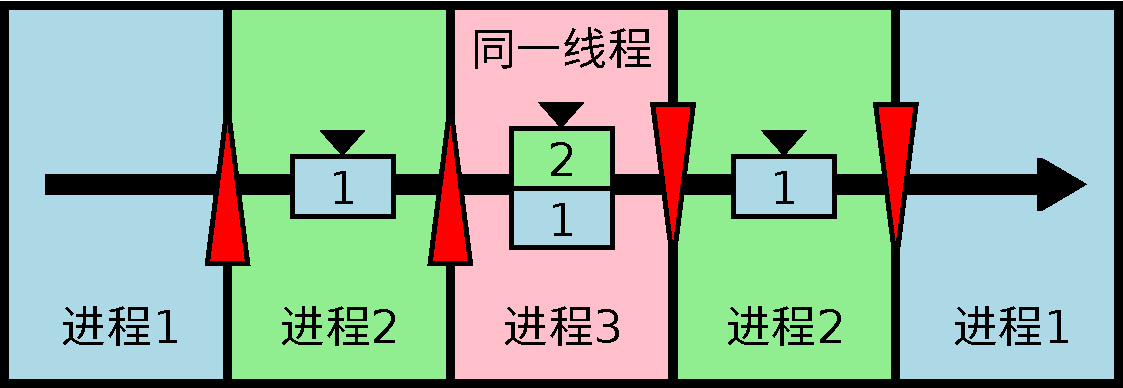
\includegraphics[width=0.72\textwidth]{Figure/image12.pdf}
    \caption{同步线程迁移示例}
    \label{fig:5-1-sync-thread-migration-example}
\end{figure}

同步迁移调用的设计参考了 Composite\hyperref[cite:5-1]{{[}1{]}}和 Mach 3\hyperref[cite:5-2]{{[}2{]}}。

\subsection{异步通信概述}\label{subsec:5-async-communication-overview}

操作系统中的异步（Asynchronous）通信机制是用来协调操作系统中的生产者-消费者（Producer-Consumer）问题的。通常而言这样的机制有邮箱（Mailbox）、消息队列（Message
Queue）等。异步通信机制的最大特点为其非阻塞性，也即一方发出后，另一方不接收，信息会先被缓存，然后发送者将直接返回。接收者在接收时，如果有信息，那么接收者返回；如果没有信息，那么接收者视系统调用的情况，可以直接返回，可以阻塞，也可以阻塞一段时间直到超时返回。

在 RME 中，异步通信模型被进一步简化为信号端点（Signal
Endpoint），其主要机制是使发送者可以向信号端点发送，使接收者可以从信号端点接收。发送总是不阻塞的，接收在有信号之时也是不阻塞的，接收在没有信号之时则可以阻塞也可以不阻塞。信号只携带数目信息\footnote{它只有一个计数器}，不携带任何其他信息。如果需要传递其他信息，那么需要在用户态通过共享内存（Shared
Memory）完成对这些信息的传递。一个异步通信的例子如下所示。其中优先级较低的线程1给优先级较高的线程2发送了一个异步信号（红色闪电标志），线程2在完成处理后又在端点上阻塞（红色长方形标志），使线程1继续执行。

\begin{figure}[htbp]
    \centering
    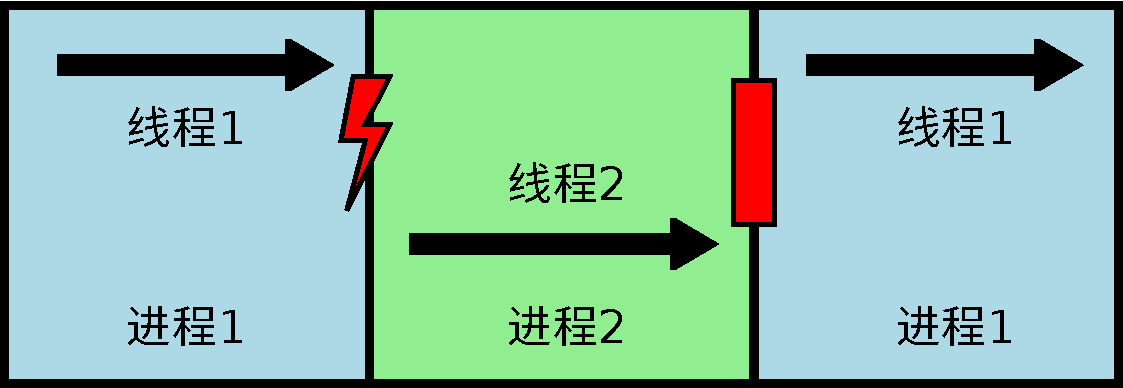
\includegraphics[width=0.72\textwidth]{Figure/image13.pdf}
    \caption{异步信号收发示例}
    \label{fig:5-2-async-signal-send-receive-example}
\end{figure}

\section{同步通信操作}\label{sec:5-sync-communication-operations}

要使用同步通信功能，那么需要先创建一个同步迁移调用。在创建同步迁移调用时，需要指明进程。在创建后，需要指定这个进程内部调用的入口和给该线程使用的栈。接下来，进行同步迁移调用，线程从一个线程内部过渡到另外一个进程之内执行。如果在这个同步迁移调用之中使用了其他的同步迁移调用，那么同步迁移调用将会进行嵌套（Nesting）。在同步迁移调用执行完毕之后，需要调用同步迁移调用返回功能，从这个迁移调用之中返回。和异步通信相比，同步通信操作具有即时性，保证在调用时一定会以最快速度得到响应，而且在进行调用时线程仅仅是跨到另外一个保护域中执行而不改变其其他属性。需要注意的是，同步迁移调用不会保存任何通用寄存器或者协处理器寄存器，也不会更改协处理器当前的状态；它只会更改那些改变程序执行流必要的寄存器，如堆栈指针和程序计数器等。通用寄存器的值和协处理器状态将会被直接带到线程迁移入口和出口。如果有需要保存的寄存器或者协处理器状态，那么需要用户态自行完成。此外，协处理器寄存器组也可以用来传递额外的参数或者接收额外的返回值。

同步迁移调用不会被绑定到CPU。如果有多个CPU上的线程试图同时激活一个同步迁移调用，那么只有一个CPU上的线程会成功，其他的线程都会返回错误码；如果在一个迁移调用被激活时试图再次激活它\footnote{不管是在同一个CPU上还是在不同的CPU上}，那么也会返回错误码。

如果同步迁移调用中发生了嵌套，那么返回时也需要逐级返回。如果线程在进行迁移调用的过程中被解除绑定，那么它仍然处于迁移调用状态，被绑定到新的CPU后会继续从那里执行；如果线程在进行迁移调用的过程中发生了一个错误，线程的行为是由设置迁移调用执行属性时传入的 Fault\_Ret\_Flag 参数决定的。如果该参数不为0，那么它并不会进入 RME\_THD\_EXCPEND 状态，而是会直接从这个迁移调用中返回到上一级，并且返回值是指示发生了错误的错误码。如果该参数为0，那么该线程会进入 RME\_THD\_EXCPEND 状态等待错误修复。

\section{异步通信操作}\label{sec:5-async-communication-operations}

要使用异步通信功能，那么需要先创建一个信号端点，然后使发送方向其发送信号，接收方从该端点接收即可。接收时，如果该端点没有信号，那么会阻塞；接收如果成功，那么返回值将会是顺利返回时的剩余信号数。

信号端点不会被绑定到CPU。如果有多个CPU上的线程同时试图阻塞在一个端点，那么只有一个会成功，其他的线程都会返回一个错误值。如果在一个线程已经阻塞在一个端点时，其他线程也试图阻塞\footnote{不管是在同一个CPU上还是在不同的CPU上}，那么其他线程的阻塞会失败。在实践中不推荐一个信号端点多接收者的使用方法，因为这往往需要相当复杂的协调。

需要注意的是，当一个线程已经阻塞在某个信号端点时，只有和被阻塞线程同一个CPU上的发送操作才能解除该线程的阻塞。其他CPU上的线程虽然也能向该端点发送，但是只能增加信号计数而无法解除阻塞。

RME 不允许初始（Init）线程接收任何信号。因为接收信号是潜在的阻塞操作，而 Init 线程一旦阻塞，RME 就无法保证能够在 CPU 空闲时找到一个线程来运行。如果既需要接收信号，又需要接收线程的时间片是无限的，那么可以新建一个线程，然后从 Init 向它进行无限传递，将其变成无限线程。

为了使应用程序的编写更加灵活，RME 允许四种不同的端点信号接收方法，分别如下：

\begin{xltabular}{\textwidth}{@{}>{\hsize=0.5583\hsize\raggedright\arraybackslash}X>{\hsize=1.4417\hsize\raggedright\arraybackslash}X@{}}
\caption{端点信号的四种接收方法}\label{tab:5-1-endpoint-signal-receive-methods}\\
\toprule
接收选项 & 意义\tabularnewline
\endfirsthead
\toprule
接收选项 & 意义\tabularnewline
\midrule
\endhead
\bottomrule
\endlastfoot
RME\_RCV\_BS &
以阻塞方式试图接收单个信号。有可能造成线程本身阻塞。\tabularnewline
RME\_RCV\_BM &
以阻塞方式试图接收多个信号。有可能造成线程本身阻塞，并且如果端点上有信号，会获取端点上全部的信号。\tabularnewline
RME\_RCV\_NS &
以非阻塞方式试图接收单个信号。该方法在端点上无信号时会立即返回。\tabularnewline
RME\_RCV\_NM &
以非阻塞方式试图接收多个信号。该方法在端点上无信号时会立即返回，并且如果端点上有信号，会获取端点上全部的信号。\tabularnewline
\end{xltabular}

\section{同步通信功能列表}\label{sec:5-sync-communication-function-list}

与同步迁移调用有关的内核功能如下：

\begin{xltabular}{\textwidth}{@{}>{\hsize=0.8854\hsize\raggedright\arraybackslash}X>{\hsize=0.6747\hsize\raggedright\arraybackslash}X>{\hsize=1.4400\hsize\raggedright\arraybackslash}X@{}}
\caption{同步通信相关内核功能}\label{tab:5-2-sync-communication-kernel-functions}\\
\toprule
调用号 & 类型 & 用途\tabularnewline
\endfirsthead
\toprule
调用号 & 类型 & 用途\tabularnewline
\midrule
\endhead
\bottomrule
\endlastfoot
RME\_SVC\_INV\_CRT & 系统调用 & 创建同步迁移调用\tabularnewline
RME\_SVC\_INV\_DEL & 系统调用 & 删除同步迁移调用\tabularnewline
RME\_SVC\_INV\_SET & 系统调用 &
设置同步迁移调用的执行属性\footnote{入口和栈}\tabularnewline
RME\_SVC\_INV\_ACT & 系统调用 &
激活\footnote{进行或调用}同步迁移调用\tabularnewline
RME\_SVC\_INV\_RET & 系统调用 & 从同步迁移调用返回\tabularnewline
\end{xltabular}

同步迁移调用权能的操作标志如下：

\begin{xltabular}{\textwidth}{@{}>{\hsize=0.9420\hsize\raggedright\arraybackslash}X>{\hsize=0.6957\hsize\raggedright\arraybackslash}X>{\hsize=1.3622\hsize\raggedright\arraybackslash}X@{}}
\caption{同步迁移调用操作标志}\label{tab:5-3-sync-invocation-operation-flags}\\
\toprule
标志 & 位 & 用途\tabularnewline
\endfirsthead
\toprule
标志 & 位 & 用途\tabularnewline
\midrule
\endhead
\bottomrule
\endlastfoot
RME\_INV\_FLAG\_SET & {[}0{]} &
允许设置该同步迁移调用的执行属性。\tabularnewline
RME\_INV\_FLAG\_ACT & {[}1{]} & 允许激活该同步迁移调用。\tabularnewline
\end{xltabular}

由于同步迁移调用返回操作是不需要同步迁移调用权能的，因此也没有该操作标志位\footnote{详见第~\ref{subsec:5-return-from-sync-invocation}~节}。

\subsection{创建同步迁移调用}\label{subsec:5-create-sync-invocation}

该操作会创建一个同步迁移调用，并将其权能放入某个已存在的权能表。新创建的同步迁移调用会引用创建时指定的进程，一旦在某进程内创建了一个同步迁移调用，那么这个进程在该同步迁移调用被删除前就不能被删除。创建同步迁移调用需要如下几个参数：

\begin{xltabular}{\textwidth}{@{}>{\hsize=0.6910\hsize\raggedright\arraybackslash}X>{\hsize=0.6910\hsize\raggedright\arraybackslash}X>{\hsize=0.6910\hsize\raggedright\arraybackslash}X>{\hsize=1.9271\hsize\raggedright\arraybackslash}X@{}}
\caption{创建同步迁移调用的所需参数}\label{tab:5-4-create-sync-invocation-parameters}\\
\toprule
参数名称 & 类型 & 域 & 描述\tabularnewline
\endfirsthead
\toprule
参数名称 & 类型 & 域 & 描述\tabularnewline
\midrule
\endhead
\bottomrule
\endlastfoot
Svc\_Num & ptr\_t & N & 必须为 RME\_SVC\_INV\_CRT。\tabularnewline
Cap\_Cpt & cid\_t & C &
一个对应于必须拥有 RME\_CPT\_FLAG\_CRT 属性的权能表权能的权能号，该权能号对应的权能指向要接受此新创建的同步迁移调用权能的权能表。该权能号可以是一级或者二级查找编码。\tabularnewline
Cap\_Kom & cid\_t & P1.D1 &
一个内核内存权能号，其标识的内核内存范围必须能够放下整个同步迁移调用对象，并且要拥有 RME\_KOM\_FLAG\_INV 属性。该权能号可以是一级或二级查找编码。\tabularnewline
Cap\_Inv & cid\_t & P1.D0 &
一个对应于接受该新创建的同步迁移调用权能的权能表的某位置的权能号。该权能号对应的权能必须是空白的。该权能号只能是一级查找编码。\tabularnewline
Cap\_Prc & cid\_t & P2 &
一个对应于必须拥有 RME\_PRC\_FLAG\_INV 属性的进程权能的权能号，该权能号对应的权能指向包含新创建的同步迁移调用的进程。该权能号可以是一级或者二级查找编码。\tabularnewline
Raddr & ptr\_t & P3 &
新创建的同步迁移调用要使用的内核起始相对虚拟地址。这个地址是相对于Cap\_Kom对应的内核权能的起始虚拟地址的。\tabularnewline
\end{xltabular}

该操作的返回值可能如下：

\begin{xltabular}{\textwidth}{@{}>{\hsize=0.8317\hsize\raggedright\arraybackslash}X>{\hsize=1.1683\hsize\raggedright\arraybackslash}X@{}}
\caption{同步迁移调用创建的可能返回值}\label{tab:5-5-create-sync-invocation-return-values}\\
\toprule
返回值 & 意义\tabularnewline
\endfirsthead
\toprule
返回值 & 意义\tabularnewline
\midrule
\endhead
\bottomrule
\endlastfoot
    0 & 操作成功。\tabularnewline
    RME\_ERR\_CPT\_RANGE & Cap\_Cpt 的一级/二级查找超出了范围。\tabularnewline
    RME\_ERR\_CPT\_RANGE & Cap\_Kom 的一级/二级查找超出了范围。\tabularnewline
    RME\_ERR\_CPT\_RANGE & Cap\_Prc 的一级/二级查找超出了范围。\tabularnewline
    RME\_ERR\_CPT\_RANGE & Cap\_Inv 的一级查找超出了范围。\tabularnewline
    RME\_ERR\_CPT\_FROZEN & Cap\_Cpt 的一级/二级查找的权能已经被冻结。\tabularnewline
    RME\_ERR\_CPT\_FROZEN & Cap\_Kom 的一级/二级查找的权能已经被冻结。\tabularnewline
    RME\_ERR\_CPT\_FROZEN & Cap\_Prc 的一级/二级查找权能已经被冻结。\tabularnewline
    RME\_ERR\_CPT\_FROZEN & Cap\_Inv 被冻结，或者其它核正在该处创建权能。\tabularnewline
    RME\_ERR\_CPT\_TYPE & Cap\_Cpt 不是权能表权能。\tabularnewline
    RME\_ERR\_CPT\_TYPE & Cap\_Kom 不是内核内存权能。\tabularnewline
    RME\_ERR\_CPT\_TYPE & Cap\_Prc 不是进程权能。\tabularnewline
    RME\_ERR\_CPT\_FLAG & Cap\_Cpt 无 RME\_CPT\_FLAG\_CRT 属性。\tabularnewline
    RME\_ERR\_CPT\_FLAG & Cap\_Kom 无 RME\_KOM\_FLAG\_INV 属性，或范围错误。\tabularnewline
    RME\_ERR\_CPT\_FLAG & Cap\_Prc 无 RME\_PRC\_FLAG\_INV 属性。\tabularnewline
    RME\_ERR\_CPT\_EXIST & Cap\_Inv 不是空白权能。\tabularnewline
    RME\_ERR\_CPT\_KOT & 分配内核内存失败。\tabularnewline
\end{xltabular}

\subsection{删除同步迁移调用}\label{subsec:5-delete-sync-invocation}

该操作会删除一个同步迁移调用。被删除的同步迁移调用必须不处于正被使用的状态。删除同步迁移调用需要如下几个参数：

\begin{xltabular}{\textwidth}{@{}>{\hsize=0.6910\hsize\raggedright\arraybackslash}X>{\hsize=0.6910\hsize\raggedright\arraybackslash}X>{\hsize=0.6910\hsize\raggedright\arraybackslash}X>{\hsize=1.9271\hsize\raggedright\arraybackslash}X@{}}
\caption{删除同步迁移调用的所需参数}\label{tab:5-6-delete-sync-invocation-parameters}\\
\toprule
参数名称 & 类型 & 域 & 描述\tabularnewline
\endfirsthead
\toprule
参数名称 & 类型 & 域 & 描述\tabularnewline
\midrule
\endhead
\bottomrule
\endlastfoot
Svc\_Num & ptr\_t & N & 必须为 RME\_SVC\_INV\_DEL。\tabularnewline
Cap\_Cpt & cid\_t & C &
一个对应于必须拥有 RME\_CPT\_FLAG\_DEL 属性的权能表权能的权能号，该权能号对应的权能指向含有正被删除的同步迁移调用权能的权能表。该权能号可以是一级或者二级查找编码。\tabularnewline
Cap\_Inv & cid\_t & P1 &
一个对应于将被删除的同步迁移调用权能的权能号。该权能号对应的必须是一个同步迁移调用权能。该权能号只能是一级查找编码。\tabularnewline
\end{xltabular}

该操作的返回值可能如下：

\begin{xltabular}{\textwidth}{@{}>{\hsize=0.7199\hsize\raggedright\arraybackslash}X>{\hsize=1.2801\hsize\raggedright\arraybackslash}X@{}}
\caption{删除同步迁移调用的可能返回值}\label{tab:5-7-delete-sync-invocation-return-values}\\
\toprule
返回值 & 意义\tabularnewline
\endfirsthead
\toprule
返回值 & 意义\tabularnewline
\midrule
\endhead
\bottomrule
\endlastfoot
    0 & 操作成功。\tabularnewline
    RME\_ERR\_CPT\_RANGE & Cap\_Cpt 的一级/二级查找超出了范围。\tabularnewline
    RME\_ERR\_CPT\_RANGE & Cap\_Inv 的一级查找超出了范围。\tabularnewline
    RME\_ERR\_CPT\_FROZEN & Cap\_Cpt 的一级/二级查找的权能已经被冻结。\tabularnewline
    RME\_ERR\_CPT\_FROZEN & Cap\_Inv 未被冻结。\tabularnewline
    RME\_ERR\_CPT\_TYPE & Cap\_Cpt 不是权能表权能。\tabularnewline
    RME\_ERR\_CPT\_TYPE & Cap\_Inv 不是同步迁移调用权能。\tabularnewline
    RME\_ERR\_CPT\_NULL & Cap\_Inv 为空白权能。\tabularnewline
    RME\_ERR\_CPT\_NULL & 两个核同时试图删除该同步迁移调用，此时未成功的核返回该值。\tabularnewline
    RME\_ERR\_CPT\_FLAG & Cap\_Cpt 无 RME\_CPT\_FLAG\_DEL 属性。\tabularnewline
    RME\_ERR\_CPT\_QUIE & Cap\_Inv 不安定。\tabularnewline
    RME\_ERR\_CPT\_REFCNT & Cap\_Inv 的引用计数不为 0，或者不为根权能。\tabularnewline
    RME\_ERR\_SIV\_ACT & 该同步迁移调用仍然处于被使用状态。\tabularnewline
\bottomrule
\end{xltabular}

\needspace{30\baselineskip}
\subsection{设置同步迁移调用执行属性}\label{subsec:5-set-sync-invocation-properties}

\needspace{20\baselineskip}
该操作会设置同步迁移调用的执行属性，也即其入口和栈。我们在设置时不关心该同步迁移调用是否已经在被使用。设置同步迁移调用的执行属性需要以下几个参数：

\begin{xltabular}{\textwidth}{@{}>{\hsize=0.7362\hsize\raggedright\arraybackslash}X>{\hsize=0.6815\hsize\raggedright\arraybackslash}X>{\hsize=0.6815\hsize\raggedright\arraybackslash}X>{\hsize=1.9007\hsize\raggedright\arraybackslash}X@{}}
\caption{设置同步迁移调用执行属性的所需参数}\label{tab:5-8-set-sync-invocation-properties-parameters}\\
\toprule
参数名称 & 类型 & 域 & 描述\tabularnewline
\endfirsthead
\toprule
参数名称 & 类型 & 域 & 描述\tabularnewline
\midrule
\endhead
Svc\_Num & ptr\_t & N & 必须为 RME\_SVC\_INV\_SET。\tabularnewline
Cap\_Inv & cid\_t & P1.D0 &
一个对应于必须拥有 RME\_INV\_FLAG\_SET 属性的同步迁移调用权能的权能号，该权能号对应的权能指向被设置执行属性的同步迁移调用。该权能号可以是一级或者二级查找编码。\tabularnewline
Entry & ptr\_t & P2 &
该线程迁移到用的入口。这个值是该同步迁移调用所在的进程内部的一个虚拟地址，同步迁移调用将从这里开始执行。\tabularnewline
Stack & ptr\_t & P3 &
该同步迁移调用的执行栈。这个值是该同步迁移调用所在的进程内部的一个虚拟地址，同步迁移调用将使用这个地址作为栈的起始。具体的栈是递增堆栈还是递减堆栈由用户态库决定。\tabularnewline
Is\_Exc\_Ret & ptr\_t & P1.D1 &
如果不为0，在迁移调用中一旦发生错误将会强制从迁移调用返回，不会允许错误修复。如果为0，则该线程将进入 RME\_THD\_EXCPEND 状态等待错误修复。\tabularnewline
\end{xltabular}

该操作的返回值可能如下：

\begin{xltabular}{\textwidth}{@{}>{\hsize=0.8188\hsize\raggedright\arraybackslash}X>{\hsize=1.1812\hsize\raggedright\arraybackslash}X@{}}
\caption{设置同步迁移调用执行属性的可能返回值}\label{tab:5-9-set-sync-invocation-properties-return-values}\\
\toprule
返回值 & 意义\tabularnewline
\endfirsthead
\toprule
返回值 & 意义\tabularnewline
\midrule
\endhead
\bottomrule
\endlastfoot
    0 & 操作成功。\tabularnewline
    RME\_ERR\_CPT\_RANGE & Cap\_Inv 的一级/二级查找超出了范围。\tabularnewline
    RME\_ERR\_CPT\_FROZEN & Cap\_Inv 的一级/二级查找的权能已经被冻结。\tabularnewline
    RME\_ERR\_CPT\_TYPE & Cap\_Inv 不是同步迁移调用权能，或者为空白权能。\tabularnewline
    RME\_ERR\_CPT\_FLAG & Cap\_Inv 无 RME\_INV\_FLAG\_SET 属性。\tabularnewline
\end{xltabular}

\subsection{激活同步迁移调用}\label{subsec:5-activate-sync-invocation}

该操作会进行一个同步迁移调用。该迁移调用必须没有被占用。进行同步迁移调用需要以下几个参数：

\begin{xltabular}{\textwidth}{@{}>{\hsize=0.6910\hsize\raggedright\arraybackslash}X>{\hsize=0.6910\hsize\raggedright\arraybackslash}X>{\hsize=0.6910\hsize\raggedright\arraybackslash}X>{\hsize=1.9271\hsize\raggedright\arraybackslash}X@{}}
\caption{激活同步迁移调用的所需参数}\label{tab:5-10-activate-sync-invocation-parameters}\\
\toprule
参数名称 & 类型 & 域 & 描述\tabularnewline
\endfirsthead
\toprule
参数名称 & 类型 & 域 & 描述\tabularnewline
\midrule
\endhead
\bottomrule
\endlastfoot
Svc\_Num & ptr\_t & N & 必须为 RME\_SVC\_INV\_ACT。\tabularnewline
Cap\_Inv & cid\_t & P1 &
一个对应于必须拥有 RME\_INV\_FLAG\_ACT 属性的同步迁移调用权能的权能号，该权能号对应的权能指向被要被激活的同步迁移调用。该权能号可以是一级或者二级查找编码。\tabularnewline
Param & ptr\_t & P2 & 要向该同步迁移调用传入的参数。\tabularnewline
\end{xltabular}

\needspace{20\baselineskip}
该操作的返回值可能如下：

\begin{xltabular}{\textwidth}{@{}>{\hsize=0.8788\hsize\raggedright\arraybackslash}X>{\hsize=1.1212\hsize\raggedright\arraybackslash}X@{}}
\caption{激活同步迁移调用的可能返回值}\label{tab:5-11-activate-sync-invocation-return-values}\\
\toprule
返回值 & 意义\tabularnewline
\endfirsthead
\toprule
返回值 & 意义\tabularnewline
\midrule
\endhead
\bottomrule
\endlastfoot
    0 & 操作成功。\tabularnewline
    RME\_ERR\_CPT\_RANGE & Cap\_Inv 的一级/二级查找超出了范围。\tabularnewline
    RME\_ERR\_CPT\_FROZEN & Cap\_Inv 的一级/二级查找的权能已经被冻结。\tabularnewline
    RME\_ERR\_CPT\_TYPE & Cap\_Inv 不是同步迁移调用权能，或者为空白权能。\tabularnewline
    RME\_ERR\_CPT\_FLAG & Cap\_Inv 无 RME\_INV\_FLAG\_ACT 属性。\tabularnewline
    RME\_ERR\_SIV\_ACT & 只有当 RME\_INV\_DEPTH\_MAX\footnote{见 7.3.2} 不为 0 时可能发生：若激活该同步迁移调用，则当前线程的总调用深度会超过该上限。\tabularnewline
    RME\_ERR\_SIV\_ACT & Cap\_Inv 已经在激活状态\footnote{其他线程正在进行调用}。\tabularnewline
    RME\_ERR\_SIV\_ACT & 两个 CPU 试图同时进行这个调用，失败的 CPU 返回该值。\tabularnewline
\end{xltabular}

\subsection{从同步迁移调用返回}\label{subsec:5-return-from-sync-invocation}

该操作从一个同步迁移调用返回。这是一个特殊操作，它不需要除了调用号和线程迁移返回值之外的其他参数。如果有多个同步迁移调用嵌套，该函数返回到上一级同步迁移调用中。如果试图在没有同步迁移调用的情况下调用该函数，则会返回一个错误码，标志着返回未成功。从同步迁移调用返回需要如下参数：

\begin{xltabular}{\textwidth}{@{}>{\hsize=1.0000\hsize\raggedright\arraybackslash}X>{\hsize=1.0000\hsize\raggedright\arraybackslash}X>{\hsize=1.0000\hsize\raggedright\arraybackslash}X>{\hsize=1.0000\hsize\raggedright\arraybackslash}X@{}}
\caption{从同步迁移调用返回的所需参数}\label{tab:5-12-return-from-sync-invocation-parameters}\\
\toprule
参数名称 & 类型 & 域 & 描述\tabularnewline
\endfirsthead
\toprule
参数名称 & 类型 & 域 & 描述\tabularnewline
\midrule
\endhead
\bottomrule
\endlastfoot
Svc\_Num & ptr\_t & N & 必须为 RME\_SVC\_INV\_RET。\tabularnewline
\end{xltabular}

该操作的返回值可能如下：

\begin{xltabular}{\textwidth}{@{}>{\hsize=0.7151\hsize\raggedright\arraybackslash}X>{\hsize=1.2849\hsize\raggedright\arraybackslash}X@{}}
\caption{从同步迁移调用返回的可能返回值}\label{tab:5-13-return-from-sync-invocation-return-values}\\
\toprule
返回值 & 意义\tabularnewline
\endfirsthead
\toprule
返回值 & 意义\tabularnewline
\midrule
\endhead
\bottomrule
\endlastfoot
    0 & 操作成功。该迁移调用立即返回，该返回值不会被调用者接收。\tabularnewline
    RME\_ERR\_SIV\_EMPTY & 试图在没有同步迁移调用的情况下调用该函数。\tabularnewline
\end{xltabular}

\section{异步通信功能列表}\label{sec:5-async-communication-function-list}

与信号端点有关的内核功能如下：

\begin{xltabular}{\textwidth}{@{}>{\hsize=1.0112\hsize\raggedright\arraybackslash}X>{\hsize=0.7705\hsize\raggedright\arraybackslash}X>{\hsize=1.2183\hsize\raggedright\arraybackslash}X@{}}
\caption{异步通信相关内核功能}\label{tab:5-14-async-communication-kernel-functions}\\
\toprule
调用号 & 类型 & 用途\tabularnewline
\endfirsthead
\toprule
调用号 & 类型 & 用途\tabularnewline
\midrule
\endhead
\bottomrule
\endlastfoot
RME\_SVC\_SIG\_CRT & 系统调用 & 创建异步信号端点\tabularnewline
RME\_SVC\_SIG\_DEL & 系统调用 & 删除异步信号端点\tabularnewline
RME\_SVC\_SIG\_SND & 系统调用 & 向异步信号端点发送信号\tabularnewline
RME\_SVC\_SIG\_RCV & 系统调用 & 从异步信号端点接收信号\tabularnewline
\end{xltabular}

信号端点权能的操作标志如下：

\begin{xltabular}{\textwidth}{@{}>{\hsize=0.9507\hsize\raggedright\arraybackslash}X>{\hsize=0.6459\hsize\raggedright\arraybackslash}X>{\hsize=1.4035\hsize\raggedright\arraybackslash}X@{}}
\caption{信号端点操作标志}\label{tab:5-15-signal-endpoint-operation-flags}\\
\toprule
标志 & 位 & 用途\tabularnewline
\endfirsthead
\toprule
标志 & 位 & 用途\tabularnewline
\midrule
\endhead
\bottomrule
\endlastfoot
RME\_SIG\_FLAG\_SND & {[}0{]} & 允许向该信号端点发送。\tabularnewline
RME\_SIG\_FLAG\_RCV\_BS & {[}1{]} &
允许从该信号端点以阻塞方式接收单个信号。\tabularnewline
RME\_SIG\_FLAG\_RCV\_BM & {[}2{]} &
允许从该信号端点以阻塞方式接收多个信号。\tabularnewline
RME\_SIG\_FLAG\_RCV\_NS & {[}3{]} &
允许从该信号端点以非阻塞方式接收单个信号。\tabularnewline
RME\_SIG\_FLAG\_RCV\_NM & {[}4{]} &
允许从该信号端点以非阻塞方式接收多个信号。\tabularnewline
RME\_SIG\_FLAG\_SCHED & {[}5{]} &
允许该端点被线程绑定用于调度器信号端点。\tabularnewline
\end{xltabular}

关于位{[}5{]}的描述，请参见\ref{subsec:4-receive-thread-scheduler-event}
。

\subsection{创建异步信号端点}\label{subsec:5-create-async-signal-endpoint}

\needspace{20\baselineskip}
该操作会创建一个信号端点，并将其权能放入某个已存在的权能表。创建信号端点需要如下几个参数：

\begin{xltabular}{\textwidth}{@{}>{\hsize=0.6910\hsize\raggedright\arraybackslash}X>{\hsize=0.6910\hsize\raggedright\arraybackslash}X>{\hsize=0.6910\hsize\raggedright\arraybackslash}X>{\hsize=1.9271\hsize\raggedright\arraybackslash}X@{}}
\caption{创建信号端点的所需参数}\label{tab:5-16-create-signal-endpoint-parameters}\\
\toprule
参数名称 & 类型 & 域 & 描述\tabularnewline
\endfirsthead
\toprule
参数名称 & 类型 & 域 & 描述\tabularnewline
\midrule
\endhead
\bottomrule
\endlastfoot
Svc\_Num & ptr\_t & N & 必须为 RME\_SVC\_SIG\_CRT。\tabularnewline
Cap\_Cpt & cid\_t & C &
一个对应于必须拥有 RME\_CPT\_FLAG\_CRT 属性的权能表权能的权能号，该权能号对应的权能指向要接受此新创建的信号端点权能的权能表。该权能号可以是一级或者二级查找编码。\tabularnewline
Cap\_Sig & cid\_t & P0 &
一个对应于接受该新创建的信号端点权能的权能表的某位置的权能号。该权能号对应的权能必须是空白的。该权能号只能是一级查找编码。\tabularnewline
\end{xltabular}

该操作的返回值可能如下：

\begin{xltabular}{\textwidth}{@{}>{\hsize=0.8317\hsize\raggedright\arraybackslash}X>{\hsize=1.1683\hsize\raggedright\arraybackslash}X@{}}
\caption{创建异步信号端点的可能返回值}\label{tab:5-17-create-signal-endpoint-return-values}\\
\toprule
返回值 & 意义\tabularnewline
\endfirsthead
\toprule
返回值 & 意义\tabularnewline
\midrule
\endhead
\bottomrule
\endlastfoot
    0 & 操作成功。\tabularnewline
    RME\_ERR\_CPT\_RANGE & Cap\_Cpt 的一级/二级查找超出了范围。\tabularnewline
    RME\_ERR\_CPT\_RANGE & Cap\_Sig 的一级查找超出了范围。\tabularnewline
    RME\_ERR\_CPT\_FROZEN & Cap\_Cpt 的一级/二级查找的权能已经被冻结。\tabularnewline
    RME\_ERR\_CPT\_FROZEN & Cap\_Sig 被冻结，或者其它核正在该处创建权能。\tabularnewline
    RME\_ERR\_CPT\_TYPE & Cap\_Cpt 不是权能表权能。\tabularnewline
    RME\_ERR\_CPT\_FLAG & Cap\_Cpt 无 RME\_CPT\_FLAG\_CRT 属性。\tabularnewline
    RME\_ERR\_CPT\_EXIST & Cap\_Sig 不是空白权能。\tabularnewline
\end{xltabular}

\subsection{删除异步信号端点}\label{subsec:5-delete-async-signal-endpoint}

该操作会删除一个信号端点。被删除的信号端点必须不处于正被使用\footnote{有线程阻塞在其上}的状态。删除信号端点需要如下几个参数：

\begin{xltabular}{\textwidth}{@{}>{\hsize=0.6910\hsize\raggedright\arraybackslash}X>{\hsize=0.6910\hsize\raggedright\arraybackslash}X>{\hsize=0.6910\hsize\raggedright\arraybackslash}X>{\hsize=1.9271\hsize\raggedright\arraybackslash}X@{}}
\caption{删除异步信号端点的所需参数}\label{tab:5-18-delete-signal-endpoint-parameters}\\
\toprule
参数名称 & 类型 & 域 & 描述\tabularnewline
\endfirsthead
\toprule
参数名称 & 类型 & 域 & 描述\tabularnewline
\midrule
\endhead
\bottomrule
\endlastfoot
Svc\_Num & ptr\_t & N & 必须为 RME\_SVC\_SIG\_DEL。\tabularnewline
Cap\_Cpt & cid\_t & C &
一个对应于必须拥有 RME\_CPT\_FLAG\_DEL 属性的权能表权能的权能号，该权能号对应的权能指向含有正被删除的信号端点权能的权能表。该权能号可以是一级或者二级查找编码。\tabularnewline
Cap\_Sig & cid\_t & P1 &
一个对应于将被删除的信号端点权能的权能号。该权能号对应的必须是一个信号端点权能。该权能号只能是一级查找编码。\tabularnewline
\end{xltabular}

该操作的返回值可能如下：

\begin{xltabular}{\textwidth}{@{}>{\hsize=0.7603\hsize\raggedright\arraybackslash}X>{\hsize=1.2397\hsize\raggedright\arraybackslash}X@{}}
\caption{删除异步信号端点的可能返回值}\label{tab:5-19-delete-signal-endpoint-return-values}\\
\toprule
返回值 & 意义\tabularnewline
\endfirsthead
\toprule
返回值 & 意义\tabularnewline
\midrule
\endhead
\bottomrule
\endlastfoot
    0 & 操作成功。\tabularnewline
    RME\_ERR\_CPT\_RANGE & Cap\_Cpt 的一级/二级查找超出了范围。\tabularnewline
    RME\_ERR\_CPT\_RANGE & Cap\_Sig 的一级查找超出了范围。\tabularnewline
    RME\_ERR\_CPT\_FROZEN & Cap\_Cpt 的一级/二级查找的权能已经被冻结。\tabularnewline
    RME\_ERR\_CPT\_FROZEN & Cap\_Sig 未被冻结。\tabularnewline
    RME\_ERR\_CPT\_TYPE & Cap\_Cpt 不是权能表权能。\tabularnewline
    RME\_ERR\_CPT\_TYPE & Cap\_Sig 不是信号端点权能。\tabularnewline
    RME\_ERR\_CPT\_NULL & Cap\_Sig 为空白权能。\tabularnewline
    RME\_ERR\_CPT\_NULL & 两个核同时试图删除该信号端点，此时未成功的核返回该值。\tabularnewline
    RME\_ERR\_CPT\_FLAG & Cap\_Cpt 无 RME\_CPT\_FLAG\_DEL 属性。\tabularnewline
    RME\_ERR\_CPT\_QUIE & Cap\_Sig 不安定。\tabularnewline
    RME\_ERR\_CPT\_REFCNT & Cap\_Sig 的引用计数不为 0，或者不为根权能。\tabularnewline
    RME\_ERR\_SIV\_ACT & 该信号端点仍然处于被使用状态。\tabularnewline
    RME\_ERR\_SIV\_CONFLICT & 该信号端点是一个内核端点，不能被删除。具体描述见下章。\tabularnewline
\end{xltabular}

\needspace{30\baselineskip}
\subsection{向异步信号端点发送信号}\label{subsec:5-send-signal-to-signal-endpoint}
\nopagebreak[4]

该操作会向一个信号端点发送信号。当有线程在该端点上阻塞时，只有与该线程相同CPU上的发送才能唤醒该线程。其他CPU也可以向该端点发送，但仅能增加计数值而不能唤醒该线程。向一个信号端点发送信号需要如下几个参数：

\begin{xltabular}{\textwidth}{@{}>{\hsize=0.6910\hsize\raggedright\arraybackslash}X>{\hsize=0.6910\hsize\raggedright\arraybackslash}X>{\hsize=0.6910\hsize\raggedright\arraybackslash}X>{\hsize=1.9271\hsize\raggedright\arraybackslash}X@{}}
\caption{向异步信号端点发送信号的所需参数}\label{tab:5-20-send-signal-parameters}\\
\toprule
参数名称 & 类型 & 域 & 描述\tabularnewline
\endfirsthead
\toprule
参数名称 & 类型 & 域 & 描述\tabularnewline
\midrule
\endhead
\bottomrule
\endlastfoot
Svc\_Num & ptr\_t & N & 必须为 RME\_SVC\_SIG\_SND。\tabularnewline
Cap\_Sig & cid\_t & P1 &
一个对应于必须拥有 RME\_SIG\_FLAG\_SND 属性的信号端点权能的权能号，该权能号对应的权能指向要对其发送信号的端点。该权能号可以是一级或者二级查找编码。\tabularnewline
Number & ptr\_t & P2 &
向信号端点发送的计数数量。一次能发送的数量上限在32位系统中为2\textsuperscript{16}，64位系统中则为2\textsuperscript{32}，依此类推。除了常规用途之外，当确信所有发送者和接收者均位于同一CPU核心、接收者优先级总是比任一发送者高时，接收者解除阻塞时会立即抢占发送者，该数字可以用来携带关于发送者身份的信息，以省去不必要的共享内存。\tabularnewline
\end{xltabular}

该操作的返回值可能如下：

\begin{xltabular}{\textwidth}{@{}>{\hsize=0.6791\hsize\raggedright\arraybackslash}X>{\hsize=1.3209\hsize\raggedright\arraybackslash}X@{}}
\caption{向异步信号端点发送信号的可能返回值}\label{tab:5-21-send-signal-return-values}\\
\toprule
返回值 & 意义\tabularnewline
\endfirsthead
\toprule
返回值 & 意义\tabularnewline
\midrule
\endhead
\bottomrule
\endlastfoot
    0 & 操作成功。\tabularnewline
    RME\_ERR\_CPT\_RANGE & Cap\_Sig 的一级/二级查找超出了范围。\tabularnewline
    RME\_ERR\_CPT\_FROZEN & Cap\_Sig 的一级/二级查找的权能已经被冻结。\tabularnewline
    RME\_ERR\_CPT\_TYPE & Cap\_Sig 不是信号端点权能，或为空白权能。\tabularnewline
    RME\_ERR\_CPT\_FLAG & Cap\_Sig 无 RME\_SIG\_FLAG\_SND 属性。\tabularnewline
    RME\_ERR\_SIV\_FULL & 发送的数量超过了一次能发送的数量上限。\tabularnewline
    RME\_ERR\_SIV\_FULL & 该信号端点的信号计数已满，不能再向其继续发送。这是很罕见的，因为在32位系统中信号计数的上限为2\textsuperscript{32-2}，64位系统中则为2\textsuperscript{64-2}，依此类推。\tabularnewline
\end{xltabular}

\subsection{从异步信号端点接收信号}\label{subsec:5-receive-signal-from-signal-endpoint}

该操作会从一个信号端点接收信号。如果该信号端点上没有信号，那么会阻塞该线程直到信号到来为止。从一个信号端点接收信号需要如下几个参数：

\begin{xltabular}{\textwidth}{@{}>{\hsize=0.6910\hsize\raggedright\arraybackslash}X>{\hsize=0.6910\hsize\raggedright\arraybackslash}X>{\hsize=0.6910\hsize\raggedright\arraybackslash}X>{\hsize=1.9271\hsize\raggedright\arraybackslash}X@{}}
\caption{从异步信号端点接收信号的所需参数}\label{tab:5-22-receive-signal-parameters}\\
\toprule
参数名称 & 类型 & 域 & 描述\tabularnewline
\endfirsthead
\toprule
参数名称 & 类型 & 域 & 描述\tabularnewline
\midrule
\endhead
\bottomrule
\endlastfoot
Svc\_Num & ptr\_t & N & 必须为 RME\_SVC\_SIG\_RCV。\tabularnewline
Cap\_Sig & cid\_t & P1 &
一个对应于必须拥有 RME\_SIG\_FLAG\_RCV 属性的信号端点权能的权能号，该权能号对应的权能指向要从其接收信号的端点。该权能号可以是一级或者二级查找编码。\tabularnewline
Option\strut
 & ptr\_t\strut
 & P2\strut
 & 接收方式选项。可以有以下四种方法：

RME\_RCV\_BS：阻塞并试图接收单个信号（Blocking Single）。

RME\_RCV\_BM：阻塞并试图接收多个信号（Blocking Multi）。

RME\_RCV\_NS：不阻塞并试图接收单个信号（Non-blocking Single）。

RME\_RCV\_NM：不阻塞并试图接收多个信号（Non-blocking Multi）。\strut
\tabularnewline
\end{xltabular}

该操作的返回值可能如下：

\begin{xltabular}{\textwidth}{@{}>{\hsize=0.7023\hsize\raggedright\arraybackslash}X>{\hsize=1.2977\hsize\raggedright\arraybackslash}X@{}}
\caption{从异步信号端点接收信号的可能返回值}\label{tab:5-23-receive-signal-return-values}\\
\toprule
返回值 & 意义\tabularnewline
\endfirsthead
\toprule
返回值 & 意义\tabularnewline
\midrule
\endhead
\bottomrule
\endlastfoot
    非负值 & 操作成功。该值为本次接收接收到的信号数量。\tabularnewline
    RME\_ERR\_CPT\_RANGE & Cap\_Sig 的一级/二级查找超出了范围。\tabularnewline
    RME\_ERR\_CPT\_FROZEN & Cap\_Sig 的一级/二级查找的权能已经被冻结。\tabularnewline
    RME\_ERR\_CPT\_TYPE & Cap\_Sig 不是信号端点权能，或为空白权能。\tabularnewline
    RME\_ERR\_CPT\_FLAG & Cap\_Sig 无对应的接收选项需要的属性。\tabularnewline
    RME\_ERR\_CPT\_FLAG & RME\_RCV\_BS 需要 RME\_SIG\_FLAG\_RCV\_BS 属性。\tabularnewline
    RME\_ERR\_CPT\_FLAG & RME\_RCV\_BM 需要 RME\_SIG\_FLAG\_RCV\_BM 属性。\tabularnewline
    RME\_ERR\_CPT\_FLAG & RME\_RCV\_NS 需要 RME\_SIG\_FLAG\_RCV\_NS 属性。\tabularnewline
    RME\_ERR\_CPT\_FLAG & RME\_RCV\_NM 需要 RME\_SIG\_FLAG\_RCV\_NM 属性。\tabularnewline
    RME\_ERR\_SIV\_BOOT & 试图让 Init 线程从端点以阻塞方式接收信号。\tabularnewline
    RME\_ERR\_SIV\_ACT & 已经有一个线程阻塞在该端点，无法接收信号。\tabularnewline
    RME\_ERR\_SIV\_ACT & 提供的接收选项不正确。\tabularnewline
    RME\_ERR\_SIV\_CONFLICT & 两个核试图同时在一个端点上进行接收，发生了冲突，需要重试。\tabularnewline
\end{xltabular}

需要注意的是，如果选择非阻塞方式，那么当该端点上无信号时，函数会直接返回0，代表此次接收没有收到任何东西。此外，如果接收选项是阻塞并试图接收多个信号，而且此次接收的确产生了阻塞，那么在阻塞解除时不论已经存在多少信号，接收的信号数目总是等于解除阻塞的那次发送。

\section{本章参考文献}\label{sec:5-references}

\protect\phantomsection\label{cite:5-1}
{[}1{]}
Q. Wang, Y. Ren, M. Scaperoth, and G. Parmer, "Speck: A kernel for
scalable predictability," in Real-Time and Embedded Technology and
Applications Symposium (RTAS), 2015 IEEE, 2015, pp. 121-132.

\protect\phantomsection\label{cite:5-2}
{[}2{]} B. Ford and J. Lepreau, "Evolving mach 3.0 to a migrating thread
model," presented at the Proceedings of the USENIX Winter 1994 Technical
Conference on USENIX Winter 1994 Technical Conference, San Francisco,
California, 1994.


\chapter{内核功能调用机制和内核异步信号}\label{ch:kernel-call-and-async-signal}

\section{内核调用机制概述}\label{sec:6-kernel-call-overview}

由于 RME 微内核的架构无关部分本身仅实现了对于多种处理器的通用功能，如果某种微处理器具备某种功能，而且该种功能只能在内核态进行操作的话，要利用这种功能就必须使用 RME 的内核调用机制。很多其他系统，例如 Composite\hyperref[cite:6-1]{{[}1{]}}和 seL4\hyperref[cite:6-2]{{[}2{]}}等，也有类似的机制。

内核功能调用（Kernel
Function）机制引入了内核调用权能，它允许调用一个用户定义好的、处理器架构相关的内核函数，并且使其运行于内核态。该权能必须在启动序列\footnote{见\ref{subsubsec:7-create-kernel-function-capability-at-boot}}中创建，而且无法删除。处理器的高精度定时器、处理器间中断和低功耗运行模式的调整等等都可以通过内核调用机制进行利用，而对于没有这些功能的处理器，内核也不强迫使用者实现这些功能，以实现最大的灵活性。

每一个具体的内核功能都对应着一个内核功能号，在进行内核功能调用时需要传入。关于具体的内核调用机制的实现，请参看下个章节的描述。

\section{内核异步信号概述}\label{sec:6-async-signal-overview}

在 RME 中，由于中断处理函数是在用户态注册的，因此需要某种机制将这些信号传导出来。RME 使用内核异步信号端点（Kernel
Asynchronous Signal
Endpoint）的方式将这些中断函数导出。内核异步信号端点和普通的信号端点是一样的，其唯一的区别是创建在系统启动时完成，并且在系统运行的整个过程中不可被删除。如果需要接收内核异步信号端点上的信号，那么只要使用与普通端点同样的接收函数到该端点上接收即可。基于同样的原因，RME 没有在内核中实现定时器，而是将时钟中断传递到用户态进行处理。

\section{内核调用机制功能列表}\label{sec:6-kernel-call-function-list}

与内核调用机制有关的内核功能如下：

\begin{xltabular}{\textwidth}{@{}>{\hsize=1.0249\hsize\raggedright\arraybackslash}X>{\hsize=0.9066\hsize\raggedright\arraybackslash}X>{\hsize=1.0685\hsize\raggedright\arraybackslash}X@{}}
\caption{内核调用相关内核功能}\label{tab:6-1-kernel-call-related-kernel-functions}\\
\toprule
调用号 & 类型 & 用途\tabularnewline
\endfirsthead
\toprule
调用号 & 类型 & 用途\tabularnewline
\midrule
\endhead
\bottomrule
\endlastfoot
RME\_SVC\_KFN & 系统调用 & 调用内核功能\tabularnewline
\end{xltabular}

\needspace{20\baselineskip}
内核调用权能的操作标志如下：

\begin{xltabular}{\textwidth}{@{}>{\hsize=0.6265\hsize\raggedright\arraybackslash}X>{\hsize=0.6265\hsize\raggedright\arraybackslash}X>{\hsize=1.7471\hsize\raggedright\arraybackslash}X@{}}
\caption{内核调用操作标志}\label{tab:6-2-kernel-call-operation-flags}\\
\toprule
标志 & 类型 & 用途\tabularnewline
\endfirsthead
\toprule
标志 & 类型 & 用途\tabularnewline
\midrule
\endhead
\bottomrule
\endlastfoot
所有位 & 位段 &
允许的内核功能范围号的范围。注意不要把内核功能号和系统调用号相混淆。在传递内核调用权能时需要使用宏 RME\_KFN\_FLAG(HIGH,LOW) 来填充新的内核调用权能的标志位，HIGH 为功能号的上限，LOW 为功能号的下限，[HIGH, LOW] 组成的闭区间即为允许内核功能号的范围。\tabularnewline
\end{xltabular}

\subsection{内核调用机制初始创建}\label{subsec:6-kernel-call-initial-creation}

关于内核调用机制的初始创建，请参见\ref{subsubsec:7-create-kernel-function-capability-at-boot}
。

\subsection{内核调用激活}\label{subsec:6-activate-kernel-call}

该操作会执行一个内核调用函数。该操作可以携带一个子功能号，还可以带两个额外参数。激活一个内核调用需要如下几个参数：

\begin{xltabular}{\textwidth}{@{}>{\hsize=0.6946\hsize\raggedright\arraybackslash}X>{\hsize=0.6946\hsize\raggedright\arraybackslash}X>{\hsize=0.6946\hsize\raggedright\arraybackslash}X>{\hsize=1.9162\hsize\raggedright\arraybackslash}X@{}}
\caption{内核调用激活的所需参数}\label{tab:6-3-kernel-call-activation-parameters}\\
\toprule
参数名称 & 类型 & 域 & 描述\tabularnewline
\endfirsthead
\toprule
参数名称 & 类型 & 域 & 描述\tabularnewline
\midrule
\endhead
\bottomrule
\endlastfoot
Svc\_Num & ptr\_t & N & 必须为 RME\_SVC\_KFN。\tabularnewline
Cap\_Kfn & cid\_t & C &
一个对应于内核调用权能的权能号。该权能号可以是一级或者二级查找编码。\tabularnewline
Func\_ID & ptr\_t & P1.D0 & 内核功能号。\tabularnewline
Sub\_ID & ptr\_t & P1.D1 & 子功能号。\tabularnewline
Param1 & ptr\_t & P2 & 传入的第一个参数。\tabularnewline
Param2 & ptr\_t & P3 & 传入的第二个参数。\tabularnewline
\end{xltabular}

该操作的返回值可能如下：

\begin{xltabular}{\textwidth}{@{}>{\hsize=0.6791\hsize\raggedright\arraybackslash}X>{\hsize=1.3209\hsize\raggedright\arraybackslash}X@{}}
\caption{内核调用激活的可能返回值}\label{tab:6-4-kernel-call-activation-return-values}\\
\toprule
返回值 & 意义\tabularnewline
\endfirsthead
\toprule
返回值 & 意义\tabularnewline
\midrule
\endhead
\bottomrule
\endlastfoot
    非负值 & 操作成功。返回值的意义由具体的底层实现决定。\tabularnewline
    RME\_ERR\_CPT\_RANGE & Cap\_Kfn 的一级/二级查找超出了范围。\tabularnewline
    RME\_ERR\_CPT\_FROZEN & Cap\_Kfn 的一级/二级查找的权能已经被冻结。\tabularnewline
    RME\_ERR\_CPT\_TYPE & Cap\_Kfn 不是内核调用权能，或为空白权能。\tabularnewline
    RME\_ERR\_CPT\_FLAG & Cap\_Kfn 的功能号范围不允许功能号为 Func\_ID 的调用。\tabularnewline
    RME\_ERR\_CPT\_NULL & 内核调用因为底层硬件不支持所传入参数而失败。该值一般不会返回，通常被返回的是用户自定义的错误码。\tabularnewline
\end{xltabular}

\section{内核异步信号功能列表}\label{sec:6-async-signal-function-list}

\subsection{内核信号端点初始创建}\label{subsec:6-kernel-signal-endpoint-initial-creation}

关于内核信号端点的初始创建，请参见\ref{subsubsec:7-create-kernel-signal-endpoint-at-boot}
。

\subsection{向内核信号端点发送信号}\label{subsec:6-send-signal-to-kernel-signal-endpoint}

关于向内核信号端点的信号发送，请参见\ref{subsubsec:7-send-signal-to-kernel-endpoint}
。

\subsection{从内核信号端点接收信号}\label{subsec:6-receive-signal-from-kernel-signal-endpoint}

从内核端点接收信号的方法和调用和普通信号端点是一样的，请参见\ref{subsec:5-receive-signal-from-signal-endpoint}
。

\section{本章参考文献}\label{sec:6-chapter-bibliography}

\protect\phantomsection\label{cite:6-1}

\noindent {[}1{]} Q. Wang, Y. Ren, M. Scaperoth, and G. Parmer, ``Speck: a kernel for scalable predictability,'' in \textit{Proceedings of the IEEE Real-Time and Embedded Technology and Applications Symposium (RTAS)}, 2015, pp. 121--132.

\protect\phantomsection\label{cite:6-2}

\noindent {[}2{]} G. Klein, K. Elphinstone, G. Heiser, J. Andronick, D. Cock, P. Derrin, et al., ``seL4: formal verification of an OS kernel,'' in \textit{Proceedings of the ACM SIGOPS 22nd Symposium on Operating Systems Principles}, Big Sky, MT, USA, 2009.


\chapter{移植RME到新架构}\label{ch:porting-rme-to-new-architecture}

\section{移植概述}\label{sec:7-porting-overview}

操作系统的移植是指将一个操作系统加以修改从而使其能运行在一个新的体系架构上的工作。有时，我们也把使得能用一款新编译器编译该操作系统的工作叫做移植工作。相比较于 Linux 等系统的移植，RME 的移植是非常简单的。RME 的所有代码都用绝大程度上符合 MISRA C 规范\footnote{为了维护工程规整性，RME 对此规范有一些必要的背离，见\ref{subsec:9-type-punning-aliasing}}的 ANSI/ISO C89 代码写成，并包含有最小量的汇编，因此其移植工作仅仅需要几步。

在移植之前，我们要先做一些准备工作，以确定移植可以进行；然后，分别针对各个部分，编写相应的移植代码即可。最后，还可以用一些测试用例来测试系统是否正确移植成功。

\section{移植前的检查工作}\label{sec:7-pre-porting-checks}

\subsection{处理器}\label{subsec:7-processor}

RME 要求所选择的处理器能够容纳一个完整的全功能操作系统。处理器必须具备较好的性能，以克服进行系统调用的开销，使全功能操作系统具有实际意义；处理器还必须具备一定的内存访问控制能力，这可以由内存管理单元（MMU）或内存保护单元（MPU）实现。

理想地，这种系统一般都是主频达到GHz级别，有百MB以上级别RAM的32位以上单核或多核微处理器平台。但是，RME 也可以支持仅有16kB
RAM和64kB ROM的32位单片机。

RME 不能在少于32kB存储器的平台上运行，也不能在低于32位的处理器上运行。此外，如果所选择的处理器没有内存保护功能，那么运行 RME 是没有意义的；在这种状况下，RMP 是一个更好的选择。最后，由于 RME 不支持硬件堆栈机制\footnote{这是 PIC 单片机等少数架构的典型实现方式}，堆栈必须是由软件实现的\footnote{也即堆栈指针可以由用户修改，堆栈实现在内存中}。

\subsection{编译器}\label{subsec:7-compiler}

RME 要求编译器是 C89 标准的，并能够根据一定的函数调用约定生成代码。由于 RME 的代码非常标准，也不使用C运行时库中的库函数，因此只要编译器符合 ANSI C89 标准即可。通常的GCC、CLANG/LLVM、MSVC、ARMCC、ICC、IAR、TASKING等编译器都是满足这个需求的。RME 没有使用位段、enum 和结构体对齐等各编译器实现差别较大的编译器扩展，也没有使用 C 语言中的未定义操作\footnote{除了某一小部分因别无他法造成的未定义行为，见\ref{subsec:9-type-punning-aliasing}}，因此保证了最大限度的兼容性。

在使用低质量编译器时，要注意关闭死代码消除功能和链接时优化功能，最好也要关闭编译器的循环不变量外提优化。某些激进的优化有可能导致中断处理向量被整个优化掉\footnote{因为在函数调用图中它们不会被任何函数调用，某些低质量链接器又不将中断向量纳入函数调用图进行分析}，引起内核无法工作，也有可能导致内核的其他功能故障。不要使用任何激进的编译优化选项，在一般的编译器上，推荐的优化选项是（如 GCC）-O2 或相当的优化水平。

\subsection{汇编器}\label{subsec:7-assembler}

RME 要求汇编器能够引入 C 中的符号，并根据函数调用约定进行调用；此外，也要求汇编器产生的代码能够导出并根据函数调用约定被 C 调用。这通常是非常好满足的要求。如果编译器可以内联汇编，那么不需要汇编器也是可以的。

\subsection{链接器}\label{subsec:7-linker}

RME 要求链接器必须具备链接多个对象\footnote{一般是 .o、.obj 或 .elf 文件}文件到一个中间对象文件的能力，而且要求能够接受定制的链接器脚本。通常的 ld、cl、armlink、ilink/xlink 等链接器都足以满足这种需求。每种链接器的链接器脚本往往都不相同，这往往需要根据每种链接器的语法决定。

\subsection{调试器}\label{subsec:7-debugger}

RME 对调试器没有特别的要求。如果有调试器可用的话，当然是最好的，但是没有调试器也是可以进行移植的。在有调试器的情况下可以直接用调试器查看内核变量；在没有调试器的情况下，要先实现内核最底层的\_\_RME\_Putchar 函数，实现单个字符的打印输出，然后就可以用该打印输出来输出日志了。关于该函数的实现请看下节所述。

\section{RME架构相关部分介绍}\label{sec:7-architecture-dependent-parts-overview}

RME 的架构相关部分代码的源文件全部都放在 Platform 文件夹的对应架构名称下。如 ARMv7-M 架构的文件夹名称为 Platform/A7M。其头文件在 Include/Platform/A7M，其他架构依此类推。

每个架构都包含一个或多个源文件和一个或多个头文件。内核包含架构相关头文件时，总是会包含 rme\_platform.h，而这是一个包含了对应架构顶层头文件的头文件。在更改 RME 的编译目标平台时，通过修改这个头文件来达成对不同目标的相应头文件的包含。比如，要针对ARMv7-M架构进行编译，那么该头文件就应该包含对应ARMv7-M的底层函数实现的全部头文件。

在移植之前，可以先浏览已有的移植，并寻找一个与目标架构的逻辑组织最相近的架构的移植。然后，可以将这个移植拷贝一份，并将其当做模板进行修改。

\subsection{类型定义}\label{subsec:7-type-definitions}

对于每个架构/编译器，首先需要移植的部分就是 RME 的类型定义。RME 的类型定义一共有下表中所示的五个，它们都以rme\_为前缀开始；为了简洁起见，在本手册中rme\_前缀均省去不写。

\begin{xltabular}{\textwidth}{@{}>{\hsize=0.5279\hsize\raggedright\arraybackslash}X>{\hsize=1.4721\hsize\raggedright\arraybackslash}X@{}}
\caption{类型定义一览}\label{tab:7-1-type-definitions-overview}\\
\toprule
类型 & 作用\tabularnewline
\endfirsthead
\toprule
类型 & 作用\tabularnewline
\midrule
\endhead
\bottomrule
\endlastfoot
    tid\_t & 线程号的类型。这个类型应该被 typedef 为与处理器字长相等的有符号整数。\newline 例子：\texttt{typedef long tid\_t;}\tabularnewline
    ptr\_t & 指针整数的类型。这个类型应该被 typedef 为与处理器字长相等的无符号整数。\newline 例子：\texttt{typedef unsigned long ptr\_t;}\tabularnewline
    cnt\_t & 计数变量的类型。这个类型应该被 typedef 为最长为一个处理器字长但至少为 32 位的有符号整数。\newline 例子：\texttt{typedef long cnt\_t;}\tabularnewline
    cid\_t & 权能号的类型。这个类型应该被 typedef 为与处理器字长相等的有符号整数。\newline 例子：\texttt{typedef long cid\_t;}\tabularnewline
    ret\_t & 函数返回值的类型。这个类型应该被 typedef 为与处理器字长相等的有符号整数。\newline 例子：\texttt{typedef long ret\_t;}\tabularnewline
\end{xltabular}

\subsection{一般宏定义}\label{subsec:7-general-macro-definitions}

其次，需要移植的是 RME 的一般宏定义。RME 的一般宏定义一共有如下几个：

\begin{xltabular}{\textwidth}{@{}>{\hsize=0.7706\hsize\raggedright\arraybackslash}X>{\hsize=1.2294\hsize\raggedright\arraybackslash}X@{}}
\caption{一般宏定义一览}\label{tab:7-2-general-macro-definitions-overview}\\
\toprule
宏名称 & 作用\tabularnewline
\endfirsthead
\toprule
宏名称 & 作用\tabularnewline
\midrule
\endhead
\bottomrule
\endlastfoot
RME\_EXTERN\strut
 & 编译器的 extern 关键字。某些编译器可能具有不标准的 extern 关键字\footnote{或者需要将一些 C++代码和内核链接起来}，此时用这个宏定义来处理它。

例子：

\#define RME\_EXTERN extern

\#define RME\_EXTERN extern "C"\strut
\tabularnewline
RME\_INLINE\strut
 & 编译器的 inline 关键字。某些编译器可能具有不标准的 inline 关键字\footnote{或者需要强迫内联某些函数}，此时用这个宏定义来处理它。

例子：

\#define RME\_INLINE inline

\#define RME\_INLINE \_\_forceinline\strut
\tabularnewline
RME\_LIKELY(X)\strut
 & 编译器的 likely 关键字，用于指导分支预测，表示此分支很有可能被执行。如果编译器有该功能，就定义此关键字；如果没有，将它定义为(X)即可。

例子：

\#define RME\_LIKELY(X) likely(X)

\#define RME\_LIKELY(X) \_\_builtin\_expect(!!(X),1)

\#define RME\_LIKELY(X) (X)\strut
\tabularnewline
RME\_UNLIKELY(X)\strut
 & 编译器的 unlikely 关键字，用于指导分支预测，表示此分支很有可能不被执行。如果编译器有该功能，就定义此关键字；如果没有，将它定义为(X)即可。

例子：

\#define RME\_UNLIKELY(X) unlikely(X)

\#define RME\_UNLIKELY(X) \_\_builtin\_expect(!!(X),0)

\#define RME\_UNLIKELY(X) (X)\strut
\tabularnewline
RME\_CPU\_LOCAL()\strut
 & 该宏返回一个指向CPU本地存储的，struct RME\_CPU\_Local*类型的指针。对于单核处理器而言，CPU本地存储可以在架构相关层中直接声明为一个变量，此宏只需要返回该变量的地址即可；对于多核处理器而言，CPU本地存储结构体需要在初始化系统时按照系统中处理器的个数动态创建。

例子：

\#define RME\_CPU\_LOCAL() \&RME\_XXX\_CPU\_Local

（某单核架构，静态分配）

\#define RME\_CPU\_LOCAL() asm("mov some\_reg, r0")

（某多核架构，动态分配，地址存储在专用段寄存器中）\strut
\tabularnewline
RME\_WORD\_ORDER\strut
 & 处理器字长（按Bit计算）对应的2的方次。比如，32位处理器对应5，64位处理器对应6，依此类推。

例子：

\#define RME\_WORD\_ORDER (5U)\strut
\tabularnewline
RME\_PGT\_PHYS\_ENABLE\strut
 & 处理器是否要求虚拟地址总是等于物理地址。通常而言，对于基于MMU的系统，这一项总是填写0，此时使用常规页表；对于微控制器等基于MPU的系统，这一项总是填写1，此时使用路径压缩页表。

例子：

\#define RME\_PGT\_PHYS\_ENABLE (1U)\strut
\tabularnewline
RME\_QUIE\_TIME\strut
 & 安定时间的长度，单位是时间片。对于单处理器，由于没有真正的并行性，各个权能总是立即安定的，此项填写``0''；对于多处理器系统，理论上此项填写的值应当超过内核最坏执行时间（WCET）的两倍大小，工程中则推荐十倍大小。通常而言，一个时间片的时长（最小100us量级）远超过内核的WCET（10us量级），因此这里填写1即可。

例子：

\#define RME\_QUIE\_TIME (1U)\strut
\tabularnewline
RME\_TIMESTAMP\strut
 & 用来判断安定时间的系统时间戳。它可以被定义为一个被时钟中断周期性递增的变量或一个自由递增计数器。

例子：

\#define RME\_TIMESTAMP RME\_Timestamp

（定义为某个变量的场合）

\#define RME\_TIMESTAMP RME\_X64\_RDTSC

（定义为读取自由递增计数器的场合）\strut
\tabularnewline
RME\_CPT\_ENTRY\_MAX\strut
 & 权能表的最大长度，单位是权能数量。由于权能表在创建和删除时都需要遍历整个表，因此此宏可通过控制权能表的大小来控制此种遍历的执行时间上限。对于那些对实时性没有过高要求或由受信任的用户态权能管理器控制权能表大小上限的场合，该值可以设置为0；否则可将该值设置为权能表大小的上限。如果该值不是0，最终的权能表大小上限由该值和处理器字长所允许的上限中较小的那一个值确定。

例子：

\#define RME\_CPT\_ENTRY\_MAX (0U)

（无限制的场合）

\#define RME\_CPT\_ENTRY\_MAX (128U)

（限制权能表大小的场合）\strut
\tabularnewline
RME\_PGT\_RAW\_ENABLE\strut
 & 用户态页表直管开关。一旦用户打开这个开关宏，则内核将不再负责页表，并将页表相关事项全权交由用户态的可信进程管理。在创建进程时，可直接指定页表的物理地址，内核将直接信任该物理地址并使用之；这为物理地址管理提供了额外的灵活性，在高并发系统或者微控制器嵌入式系统均可使用。具体地，页表系统调用和内核功能调用将消失，RME\_SVC\_PRC\_CRT 和 RME\_SVC\_PRC\_PGT 系统调用的参数将发生变化，且内核将不再调用除 \_\_RME\_Pgt\_Set 和 \_\_RME\_Pgt\_Kom\_Init 之外的页表底层函数；\_\_RME\_Pgt\_Set的参数亦有变化。具体细节请参见相关章节。

例子：

\#define RME\_PGT\_RAW\_ENABLE (0U)

（内核管理页表的场合）

\#define RME\_PGT\_RAW\_ENABLE (1U)

（用户态可信进程直接管理页表的场合）\strut
\tabularnewline
RME\_KOM\_VA\_BASE\strut
 & 用户可分配的内核虚拟内存的起始地址。填写内核虚拟内存的起始地址即可。创建内核对象时，将从这里开始分配内核内存，并且将这些分配记录在内核内存登记表中。

例子：

\#define RME\_KOM\_VA\_BASE (0xC0000000U)\strut
\tabularnewline
RME\_KOM\_VA\_SIZE\strut
 & 用户可分配的内核虚拟内存的地址空间的大小。填写内核虚拟内存的地址空间大小即可。对于那些需要动态探测内核虚拟内存空间大小的场合\footnote{比如 x86-64 等}，这里填写内核允许的最小大小\footnote{如果探测到比这个大小还小的可用内核内存虚拟地址空间，内核可以拒绝启动}。该宏主要用于在那些内核虚拟内存大小固定的场合间接指定内核内存分配表的大小（如决定RME\_KOT\_WORD\_NUM的值等）；对于那些动态探测内核虚拟内存空间大小的场合并无实际意义。

例子：

\#define RME\_KOM\_VA\_SIZE (0x30000000U)\strut
\tabularnewline
RME\_KOM\_SLOT\_ORDER\strut
 & 内核虚拟内存分配粒度对应的2的方次。比如如果内核内存分配的最小粒度为16Byte，那么这个位置要填写的数字就是log\textsubscript{2}(16)
= 4。需要注意的是，内存分配的最小粒度不能小于一个处理器字长。

例子：

\#define RME\_KOM\_SLOT\_ORDER (4U)\strut
\tabularnewline
RME\_HYP\_VA\_BASE\strut
 & 虚拟机监视器专用虚拟内存的起始地址。这段内存是给虚拟机监视器使用的，可以设置线程的虚拟化属性到这段地址，以使其寄存器在线程切换时被保存至此。

例子：

\#define RME\_HYP\_VA\_BASE (0x01000000U)\strut
\tabularnewline
RME\_HYP\_VA\_SIZE\strut
 & 虚拟机监视器专用虚拟内存的大小。填写虚拟机专用虚拟内存的实际大小即可。如果不使用这个功能，那么该宏的大小需要设置为0，此时宏 RME\_HYP\_VA\_BASE 也无效。

例子：

\#define RME\_HYP\_VA\_SIZE (0x00010000U)\strut
\tabularnewline
RME\_KSTK\_VA\_BASE\strut
 & 内核堆栈段初始虚拟地址。这是内核启动时使用的堆栈，并不总是代表运行时堆栈；在多核系统上，每个CPU运行的内核代码可能会被安排新的堆栈。

例子：

\#define RME\_KSTK\_VA\_BASE (0xF0000000U)\strut
\tabularnewline
RME\_KSTK\_VA\_SIZE\strut
 & 内核堆栈段初始长度。

例子：

\#define RME\_KSTK\_VA\_SIZE (0x1000U)\strut
\tabularnewline
RME\_PREEMPT\_PRIO\_NUM\strut
 & 内核支持的抢占优先级的最大数量。这个数量必须是处理器字长（按Bit计算）的整数倍，而且不超过处理器字长四分之一对应的2的方次，如32位处理器不超过2\textsuperscript{8}，64位处理器不超过2\textsuperscript{16}。通常而言，把这个值定义为处理器字长就够用了。

例子：

\#define RME\_PREEMPT\_PRIO\_NUM (32U)\strut
\tabularnewline
RME\_PGT\_SIZE\_NOM(X) &
处理器非顶层页目录的大小。这个宏会接受一个参数，该参数的意义是该页目录的表项数目对应的2的方次。如果该页目录中含有1024个表项，那么X的值即为10，此时该宏为 RME\_PGT\_SIZE\_NOM(10)，它会返回该页表的大小，单位为字节。如果每个页表表项的大小是4字节，附加在页表上的附加前置数据\footnote{仅在使用MPU时存在}的大小为4096字节，那么该宏应当返回8192。\tabularnewline
RME\_PGT\_SIZE\_TOP(X) &
处理器顶层页目录的大小。这个宏会接受一个参数，该参数的意义是该页目录的表项数目对应的2的方次。这个宏实际上等于 RME\_PGT\_SIZE\_NOM(X) 加上顶层额外的附加数据\footnote{仅在使用MPU时存在}的大小。\tabularnewline
RME\_KOT\_VA\_BASE\strut
 & 内核内存登记表所在的内核虚拟内存地址。对于大部分架构，直接将该宏定义为一个大小为 RME\_KOT\_WORD\_NUM 的数组的首地址即可；对于小部分拥有极高内存量的架构\footnote{如最新的 x86-64 可以有上百TB内存}，因为 GCC 等编译器最多默认放置内核到高2GB，内核内存登记表的大小会被限制在2GB，此时最多支持1TB内核内存。因此此时需要重定位该登记表，将其指向不受限制的地址，该地址可以由链接器脚本指定。

例子：

\#define RME\_KOT\_VA\_BASE RME\_XXX\_Kot

（小内核内存分配表）

\#define RME\_KOT\_VA\_BASE ((ptr\_t*)0xFFFF800001000000U)

（大内核内存分配表）\strut
\tabularnewline
RME\_INV\_DEPTH\_MAX\strut
 & 线程迁移调用的最深深度限制。这一限制是为了确保线程删除操作的最坏执行时间可控，因为它需要逐层脱去线程当前正在进行的迁移调用。对于那些对实时性没有过高要求或从不删除线程的场合，该值可以设置为0；否则可将该值设置为迁移调用深度的上限。

例子：

\#define RME\_INV\_DEPTH\_MAX (0U)

（无限制的场合）

\#define RME\_INV\_DEPTH\_MAX (32U)

（限制迁移调用深度的场合）\strut
\tabularnewline
RME\_ASSERT\_FAILED(F,L,D,T)\strut
 & 断言失败处理。在内核中一旦发生断言失败，就意味着内核彻底崩溃，必须完全复位重启，具体的处理方法与架构有关。该宏的四个参数分别是 C 预处理器提供的 \_\_FILE\_\_、\_\_LINE\_\_、\_\_DATE\_\_ 和 \_\_TIME\_\_，如果用户希望使用这四个参数，那么可以从这里读取。

例子：

\#define RME\_ASSERT\_FAILED(F,L,D,T) \_\_reboot\_processor()\strut
\tabularnewline
RME\_COP\_NUM\strut
 & 系统中协处理器的数量。如果内核支持协处理器，将它设置为大于0的数值即可。内核代码会根据该值是否为0来判断是否需要链接协处理器相关函数，但内核运行时并不关心这个数字的具体数值。

\#define RME\_COP\_NUM (1U)\strut
\tabularnewline
\end{xltabular}

\subsection{特殊宏定义}\label{subsec:7-special-macro-definitions}

这些宏定义仅在微控制器平台上出现，对于微处理器平台是无意义的。它们是配合 RVM 虚拟机监视器使用的，且这些宏定义可以由RVM配套的工程生成器来填充。有关RVM的相关信息，请查阅RVM的手册。

\begin{xltabular}{\textwidth}{@{}>{\hsize=0.7337\hsize\raggedright\arraybackslash}X>{\hsize=1.2663\hsize\raggedright\arraybackslash}X@{}}
\caption{特殊宏定义一览}\label{tab:7-3-special-macro-definitions-overview}\\
\toprule
宏名称 & 作用\tabularnewline
\endfirsthead
\toprule
宏名称 & 作用\tabularnewline
\midrule
\endhead
\bottomrule
\endlastfoot
RME\_RVM\_INIT\_CPT\_SIZE\strut
 & 内核启动时创建的初始权能表的大小。

例子：

\#define RME\_RVM\_INIT\_CPT\_SIZE (54U)\strut
\tabularnewline
RME\_RVM\_CPT\_BOOT\_FRONT\strut
 & 在内核启动后的初始权能表水位。在该水位以后，所有的权能都是空的，RVM将使用它们来创建内核对象。内核本身并不使用这个宏；用户可以在内核启动后检查占用的权能是否超过该水位，若超过该水位则报错。

例子：

\#define RME\_RVM\_CPT\_BOOT\_FRONT RVM\_CAP\_NUM\strut
\tabularnewline
RME\_RVM\_KOM\_BOOT\_FRONT\strut
 & 在内核启动后的内核内存水位，是一个相对于RME\_KOM\_VA\_BASE的值。内核本身并不使用这个宏；用户可以在内核启动后检查占用的内核内存是否超过该水位，若超过该水位则报错。

\#define RME\_RVM\_KOM\_BOOT\_FRONT RVM\_KOM\_ADDR\strut
\tabularnewline
RME\_RVM\_CPT\_DONE\_FRONT\strut
 & 在RVM完成一切内核对象创建后的初始权能表水位。在该水位以后，所有的权能都是空的，用户可以使用它们来创建内核对象。内核本身并不使用这个宏；这个宏是为了用户编写启动代码方便而提供的。

例子：

\#define RME\_RVM\_CPT\_DONE\_FRONT USER\_CAP\_NUM\strut
\tabularnewline
RME\_RVM\_KOM\_DONE\_FRONT\strut
 & 在内核启动后的内核内存水位，是一个相对于RME\_KOM\_VA\_BASE的值。内核本身并不使用这个宏；这个宏是为了用户编写启动代码方便而提供的。用户可以在启动后检查占用的内核内存是否超过该水位，若超过该水位则报错。

\#define RME\_RVM\_KOM\_DONE\_FRONT USER\_KOM\_ADDR\strut
\tabularnewline
RME\_RVM\_PHYS\_VCT\_NUM &
物理中断的数量。该宏将由工程生成器根据芯片实况填充。\tabularnewline
RME\_RVM\_PHYS\_VCTF\_BASE &
物理中断标志位占存区的起始位置以及大小。用以通知虚拟机监视器物理中断的发生。该宏将由工程生成器负责填充。\tabularnewline
RME\_RVM\_PHYS\_VCTF\_SIZE &\tabularnewline
RME\_RVM\_VIRT\_EVT\_NUM &
事件源的数量。该宏将由工程生成器根据工程配置填充。\tabularnewline
RME\_RVM\_VIRT\_EVTF\_BASE &
事件源标志位占存区的起始位置以及大小。用以通知虚拟机监视器事件源刺激的发生。该宏将由工程生成器负责填充。\tabularnewline
RME\_RVM\_VIRT\_EVTF\_SIZE &\tabularnewline
\end{xltabular}

\subsection{调试开关宏定义}\label{subsec:7-debug-switch-macro-definitions}

这些宏定义与内核调试打印有关。它们的值可以决定内核调试功能的开启与否。

\begin{xltabular}{\textwidth}{@{}>{\hsize=0.6791\hsize\raggedright\arraybackslash}X>{\hsize=1.3209\hsize\raggedright\arraybackslash}X@{}}
\caption{调试开关宏定义一览}\label{tab:7-4-debug-switch-macro-definitions-overview}\\
\toprule
宏名称 & 作用\tabularnewline
\endfirsthead
\toprule
宏名称 & 作用\tabularnewline
\midrule
\endhead
\bottomrule
\endlastfoot
RME\_ASSERT\_ENABLE\strut
 & 控制断言宏是否开启。如果需要启用RME\_ASSERT宏以检测错误，请将其定义为1，否则可将其定义为0，此时断言将不被检查。

例子：

\#define RME\_ASSERT\_ENABLE (1U)\strut
\tabularnewline
RME\_DBGLOG\_ENABLE\strut
 & 控制以RME\_DBG\_为前缀的各个调试打印宏是否开启。如果需要在内核中调试打印，请将其定义为1。

例子：

\#define RME\_DBGLOG\_ENABLE (1U)\strut
\tabularnewline
\end{xltabular}

\subsection{架构相关结构体}\label{subsec:7-architecture-dependent-structs}

RME 的架构相关结构体一共有三个，分别如下：

\begin{xltabular}{\textwidth}{@{}>{\hsize=0.6447\hsize\raggedright\arraybackslash}X>{\hsize=1.3553\hsize\raggedright\arraybackslash}X@{}}
\caption{架构相关结构体一览}\label{tab:7-5-architecture-dependent-structs-overview}\\
\toprule
结构体 & 意义\tabularnewline
\endfirsthead
\toprule
结构体 & 意义\tabularnewline
\midrule
\endhead
\bottomrule
\endlastfoot
RME\_Reg\_Struct &
进入中断函数时寄存器压栈的结构体，包含了CPU的各个寄存器。\tabularnewline
RME\_Exc\_Struct &
与异常处理相关（包含异常原因和地址等）的结构体，包含了其各个寄存器。\tabularnewline
RME\_Iret\_Struct &
与程序执行流相关的，在同步迁移调用中要保存和恢复的寄存器的结构体。\tabularnewline
\end{xltabular}

这三个结构体的实现和系统中断向量进入段汇编函数的实现有关。

\subsection{汇编底层函数}\label{subsec:7-assembly-low-level-functions}

RME 仅要求用汇编或内联汇编实现4个短小的底层汇编函数。这些函数的名称和意义如下：

\begin{xltabular}{\textwidth}{@{}>{\hsize=1.0701\hsize\raggedright\arraybackslash}X>{\hsize=0.9299\hsize\raggedright\arraybackslash}X@{}}
\caption{汇编底层函数一览}\label{tab:7-6-assembly-low-level-functions-overview}\\
\toprule
函数名 & 意义\tabularnewline
\endfirsthead
\toprule
函数名 & 意义\tabularnewline
\midrule
\endhead
\bottomrule
\endlastfoot
主函数(main)或程序入口点 & 内核程序的入口点。\tabularnewline
\_\_RME\_Int\_Disable & 禁止处理器中断。\tabularnewline
\_\_RME\_Int\_Enable & 使能处理器中断。\tabularnewline
\_\_RME\_User\_Enter & 进入用户态执行。\tabularnewline
\end{xltabular}

这些函数的具体实现方法和实现次序将在后面章节加以讲解。

\subsection{系统中断向量}\label{subsec:7-system-interrupt-vectors}

RME 最低仅仅要求用汇编或内联汇编实现3个中断向量。这些中断向量的名称和意义如下：

\begin{xltabular}{\textwidth}{@{}>{\hsize=0.8317\hsize\raggedright\arraybackslash}X>{\hsize=1.1683\hsize\raggedright\arraybackslash}X@{}}
\caption{系统中断向量一览}\label{tab:7-7-system-interrupt-vectors-overview}\\
\toprule
中断向量名 & 意义\tabularnewline
\endfirsthead
\toprule
中断向量名 & 意义\tabularnewline
\midrule
\endhead
\bottomrule
\endlastfoot
系统定时器中断向量 & 处理系统定时器中断，管理时间片使用。\tabularnewline
系统调用中断向量 & 处理系统调用时使用。\tabularnewline
系统错误中断向量 & 发生访存错误及其他处理器错误时使用。\tabularnewline
\end{xltabular}

这些中断向量的具体实现方法和实现次序将在后面章节加以讲解。

\subsection{其他底层函数}\label{subsec:7-other-low-level-functions}

这些底层函数涉及到页表、处理器特殊功能等其他方面。这些函数可以用汇编实现，也可以不用汇编实现，也可以部分使用 C 语言，部分使用内联汇编实现。这些函数的可以分成如下几类：

\subsubsection{内核调试打印函数}\label{subsubsec:7-kernel-debug-print-function}

\begin{xltabular}{\textwidth}{@{}>{\hsize=0.7990\hsize\raggedright\arraybackslash}X>{\hsize=1.2010\hsize\raggedright\arraybackslash}X@{}}
\caption{内核调试打印函数一览}\label{tab:7-8-kernel-debug-print-function-overview}\\
\toprule
函数 & 意义\tabularnewline
\endfirsthead
\toprule
函数 & 意义\tabularnewline
\midrule
\endhead
\bottomrule
\endlastfoot
\_\_RME\_Putchar & 打印一个字符到内核调试控制台。\tabularnewline
\end{xltabular}

\subsubsection{处理器特殊功能宏定义}\label{subsubsec:7-processor-special-function-macros}

\begin{xltabular}{\textwidth}{@{}>{\hsize=0.8541\hsize\raggedright\arraybackslash}X>{\hsize=1.1459\hsize\raggedright\arraybackslash}X@{}}
\caption{处理器特殊功能宏定义一览}\label{tab:7-9-processor-special-function-macros-overview}\\
\toprule
宏定义/函数 & 意义\tabularnewline
\endfirsthead
\toprule
宏定义/函数 & 意义\tabularnewline
\midrule
\endhead
\bottomrule
\endlastfoot
RME\_READ\_ACQUIRE & 读获取操作。\tabularnewline
RME\_WRITE\_RELEASE & 写释放操作。\tabularnewline
RME\_COMP\_SWAP & 比较交换原子操作。\tabularnewline
RME\_FETCH\_ADD & 加载自增原子操作。\tabularnewline
RME\_FETCH\_AND & 加载逻辑与原子操作。\tabularnewline
RME\_MSB\_GET & 得到一个字的最高位（MSB）位置。\tabularnewline
\end{xltabular}

\subsubsection{初始化与启动函数}\label{subsubsec:7-init-and-boot-functions}

\begin{xltabular}{\textwidth}{@{}>{\hsize=0.8787\hsize\raggedright\arraybackslash}X>{\hsize=1.1213\hsize\raggedright\arraybackslash}X@{}}
\caption{初始化与启动函数一览}\label{tab:7-10-init-and-boot-functions-overview}\\
\toprule
函数 & 意义\tabularnewline
\endfirsthead
\toprule
函数 & 意义\tabularnewline
\midrule
\endhead
\bottomrule
\endlastfoot
\_\_RME\_Lowlvl\_Init & 底层硬件初始化。\tabularnewline
\_\_RME\_Boot & 创建初始内核对象并启动系统。\tabularnewline
\end{xltabular}

\subsubsection{寄存器组相关函数}\label{subsubsec:7-register-set-functions}

\begin{xltabular}{\textwidth}{@{}>{\hsize=0.8554\hsize\raggedright\arraybackslash}X>{\hsize=1.1446\hsize\raggedright\arraybackslash}X@{}}
\caption{寄存器组相关函数一览}\label{tab:7-11-register-set-functions-overview}\\
\toprule
函数 & 意义\tabularnewline
\endfirsthead
\toprule
函数 & 意义\tabularnewline
\midrule
\endhead
\bottomrule
\endlastfoot
\_\_RME\_Svc\_Param\_Get & 从寄存器组中得到系统调用参数。\tabularnewline
\_\_RME\_Svc\_Retval\_Set &
向寄存器组中设置系统调用的返回值。\tabularnewline
\_\_RME\_Thd\_Reg\_Init &
初始化线程或迁移调用的寄存器组。\tabularnewline
\_\_RME\_Thd\_Reg\_Copy &
将一个寄存器组拷贝到另一个寄存器组。\tabularnewline
\_\_RME\_Thd\_Reg\_Print &
打印线程的寄存器组；仅作调试用。\tabularnewline
\_\_RME\_Thd\_Cop\_Init & 初始化线程的协处理器寄存器组。\tabularnewline
\_\_RME\_Thd\_Cop\_Swap &
保存和恢复线程的协处理器寄存器组。\tabularnewline
\_\_RME\_Inv\_Reg\_Save &
保存同步迁移调用返回用的必要寄存器。\tabularnewline
\_\_RME\_Inv\_Reg\_Restore &
恢复同步迁移调用返回用的必要寄存器。\tabularnewline
\_\_RME\_Inv\_Retval\_Set &
向寄存器组中设置同步迁移调用的返回值。\tabularnewline
\end{xltabular}

\subsubsection{协处理器寄存器组相关函数}\label{subsubsec:7-coprocessor-register-set-functions}



\begin{xltabular}{\textwidth}{@{}>{\hsize=0.8317\hsize\raggedright\arraybackslash}X>{\hsize=1.1683\hsize\raggedright\arraybackslash}X@{}}
\caption{协处理器寄存器组相关函数一览}\label{tab:7-12-coprocessor-register-set-functions-overview}\\
\toprule
函数 & 意义\tabularnewline
\endfirsthead
\toprule
函数 & 意义\tabularnewline
\midrule
\endhead
\bottomrule
\endlastfoot
\_\_RME\_Thd\_Reg\_Init &
初始化线程或迁移调用的寄存器组。\tabularnewline
\_\_RME\_Thd\_Reg\_Copy &
将一个寄存器组拷贝到另一个寄存器组。\tabularnewline
\_\_RME\_Thd\_Cop\_Init & 初始化线程的协处理器寄存器组。\tabularnewline
\_\_RME\_Thd\_Cop\_Swap &
保存和恢复线程的协处理器寄存器组。\tabularnewline
\end{xltabular}

\subsubsection{内核功能调用函数}\label{subsubsec:7-kernel-function-call-functions}

\begin{xltabular}{\textwidth}{@{}>{\hsize=0.9605\hsize\raggedright\arraybackslash}X>{\hsize=1.0395\hsize\raggedright\arraybackslash}X@{}}
\caption{内核功能调用函数一览}\label{tab:7-13-kernel-function-call-functions-overview}\\
\toprule
函数 & 意义\tabularnewline
\endfirsthead
\toprule
函数 & 意义\tabularnewline
\midrule
\endhead
\bottomrule
\endlastfoot
\_\_RME\_Kfn\_Handler & 内核功能调用的实现。\tabularnewline
\end{xltabular}

\needspace{30\baselineskip}
\subsubsection{页表相关函数}\label{subsubsec:7-page-table-functions}
\nopagebreak[4]

\begin{xltabular}{\textwidth}{@{}>{\hsize=0.7716\hsize\raggedright\arraybackslash}X>{\hsize=1.2284\hsize\raggedright\arraybackslash}X@{}}
\caption{页表相关函数一览}\label{tab:7-14-page-table-functions-overview}\\
\toprule
函数 & 意义\tabularnewline
\endfirsthead
\toprule
函数 & 意义\tabularnewline
\midrule
\endhead
\bottomrule
\endlastfoot
\_\_RME\_Pgt\_Set &
切换当前使用的页表\footnote{顶层页目录}。\tabularnewline
\_\_RME\_Pgt\_Kom\_Init & 初始化内核页表。\tabularnewline
\_\_RME\_Pgt\_Check & 检查页目录参数是否能被本架构支持。\tabularnewline
\_\_RME\_Pgt\_Init & 初始化页目录。\tabularnewline
\_\_RME\_Pgt\_Del\_Check & 检查该页目录是否能被删除。\tabularnewline
\_\_RME\_Pgt\_Page\_Map & 映射一个页到页目录内。\tabularnewline
\_\_RME\_Pgt\_Page\_Unmap & 从页目录内删除一个页的映射。\tabularnewline
\_\_RME\_Pgt\_Pgdir\_Map &
映射一个子页目录到一个父页目录内。\tabularnewline
\_\_RME\_Pgt\_Pgdir\_Unmap &
从父页目录内删除一个子页目录的映射。\tabularnewline
\_\_RME\_Pgt\_Lookup &
在一个页目录内根据相对位置查找一个物理地址页。\tabularnewline
\_\_RME\_Pgt\_Walk &
从顶层页目录开始查找一个虚拟地址对应的物理地址页属性。\tabularnewline
\end{xltabular}

\section{类型定义与汇编底层函数的移植}\label{sec:7-type-definition-and-assembly-function-porting}

对于类型定义，只需要确定处理器的字长在编译器中的表达方法，使用 typedef 定义即可。需要注意的是，对于某些架构和编译器，long（长整型）类型对应的是两个机器字的长度，而非一个机器字；此时应当使用 int 类型来表达一个机器字的长度。对于另一些架构和编译器，int 是半个机器字的长度，long 是一个机器字的长度，此时应当注意用 long 来定义一个机器字。

在必要的时候，可以使用 sizeof() 运算符编写几个小程序，来确定该编译器的机器字究竟是何种标准。

为了使得底层函数的编写更加方便，推荐使用如下的几个 typedef 来定义经常使用到的确定位数的整形。在定义这些整形时，也需要确定编译器的 char、short、int、long 等究竟是多少个机器字的长度。有些编译器不提供六十四位或者一百二十八位整数，那么这几个类型可以略去。

\begin{xltabular}{\textwidth}{@{}>{\hsize=0.6576\hsize\raggedright\arraybackslash}X>{\hsize=1.3424\hsize\raggedright\arraybackslash}X@{}}
\caption{常用类型一览}\label{tab:7-15-common-types-overview}\\
\toprule
类型 & 意义\tabularnewline
\endfirsthead
\toprule
类型 & 意义\tabularnewline
\midrule
\endhead
\bottomrule
\endlastfoot
s8\_t\strut
 & 一个有符号八位整形。

例如：\texttt{typedef char s8\_t};\strut
\tabularnewline
s16\_t\strut
 & 一个有符号十六位整形。

例如：\texttt{typedef short s16\_t};\strut
\tabularnewline
s32\_t\strut
 & 一个有符号三十二位整形。

例如：\texttt{typedef int s32\_t};\strut
\tabularnewline
s64\_t\strut
 & 一个有符号六十四位整形。

例如：\texttt{typedef long s64\_t};\strut
\tabularnewline
s128\_t\strut
 & 一个有符号一百二十八位整形。

例如：\texttt{typedef long long s128\_t};\strut
\tabularnewline
u8\_t\strut
 & 一个无符号八位整形。

例如：\texttt{typedef unsigned char u8\_t};\strut
\tabularnewline
u16\_t\strut
 & 一个无符号十六位整形。

例如：\texttt{typedef unsigned short u16\_t};\strut
\tabularnewline
u32\_t\strut
 & 一个无符号三十二位整形。

例如：\texttt{typedef unsigned int u32\_t};\strut
\tabularnewline
u64\_t\strut
 & 一个无符号六十四位整形。

例如：\texttt{typedef unsigned long u64\_t};\strut
\tabularnewline
u128\_t\strut
 & 一个无符号一百二十八位整形。

例如：\texttt{typedef unsigned long long u128\_t};\strut
\tabularnewline
\end{xltabular}

对于宏定义和结构体类型的定义，需要根据具体系统的配置来决定。具体的决定方法见上节所述，依表格说明填充这些定义即可。

接下来说明对于汇编底层函数的移植过程。

\subsection{内核入口点的实现}\label{subsec:7-kernel-entry-point-implementation}

内核入口点完成一系列准备工作，然后调用RME\_Kmain函数。对于不同的架构和工具链，内核入口点的写法也有所不同，需要自行发挥。在调用RME\_Kmain之前，需要进行如下准备工作：

\begin{enumerate}
\def\labelenumi{\arabic{enumi}.}
\item
  将内核的各个部分通过启动器（Bootloader）正确地加载到内存中，并将处理器置于特权态。
\item
  建立最初的系统启动用页表，并使用该页表将系统切换到保护模式。该页表只要实现了内核内存的虚拟地址到内核内存的物理地址的映射即可。这个临时页表仅仅在启动过程中使用一次，在之后就不再使用了，因此在系统启动完成后可以将其删除。
\item
  根据 RME\_KSTK\_VA\_BASE 和 RME\_KSTK\_VA\_SIZE 设置正确的内核堆栈指针。
\end{enumerate}

\subsection{\_\_RME\_Int\_Disable的实现}\label{subsec:7-rme-int-disable-implementation}

该函数需要关闭处理器的中断，然后返回。实现上没有特别需要注意的地方，通常而言只需要写一个CPU寄存器或者外设地址，关闭中断，然后返回即可。

\begin{xltabular}{\textwidth}{@{}>{\hsize=0.7236\hsize\raggedright\arraybackslash}X>{\hsize=1.2764\hsize\raggedright\arraybackslash}X@{}}
\caption{\_\_RME\_Int\_Disable的实现}\label{tab:7-16-rme-int-disable-implementation}\\
\toprule
原型 & void \_\_RME\_Int\_Disable(void)\tabularnewline
\endfirsthead
\toprule
原型 & void \_\_RME\_Int\_Disable(void)\tabularnewline
\midrule
\endhead
\bottomrule
\endlastfoot
意义 & 关闭处理器中断。\tabularnewline
返回值 & 无。\tabularnewline
参数 & 无。\tabularnewline
\end{xltabular}

\subsection{\_\_RME\_Int\_Enable的实现}\label{subsec:7-rme-int-enable-implementation}

该函数需要开启处理器的中断，然后返回。实现上没有特别需要注意的地方，通常而言只需要写一个CPU寄存器或者外设地址，开启中断，然后返回即可。

\begin{xltabular}{\textwidth}{@{}>{\hsize=0.7321\hsize\raggedright\arraybackslash}X>{\hsize=1.2679\hsize\raggedright\arraybackslash}X@{}}
\caption{\_\_RME\_Int\_Enable的实现}\label{tab:7-17-rme-int-enable-implementation}\\
\toprule
原型 & void \_\_RME\_Int\_Enable(void)\tabularnewline
\endfirsthead
\toprule
原型 & void \_\_RME\_Int\_Enable(void)\tabularnewline
\midrule
\endhead
\bottomrule
\endlastfoot
意义 & 开启处理器中断。\tabularnewline
返回值 & 无。\tabularnewline
参数 & 无。\tabularnewline
\end{xltabular}

\subsection{\_\_RME\_User\_Enter的实现}\label{subsec:7-rme-user-enter-implementation}

该函数实现从特权态到用户态的切换，仅在系统启动阶段的最后被调用。在此之后，系统进入正常运行状态。该函数只要将 Stack 的值赋给堆栈指针，将 CPUID 赋给调用约定决定的第一个参数的寄存器，然后直接跳转到 Entry 并进行处理器状态切换即可。该函数将永远不会返回。

\begin{xltabular}{\textwidth}{@{}>{\hsize=0.5670\hsize\raggedright\arraybackslash}X>{\hsize=1.4330\hsize\raggedright\arraybackslash}X@{}}
\caption{\_\_RME\_User\_Enter的实现}\label{tab:7-18-rme-user-enter-implementation}\\
\toprule
原型 & void \_\_RME\_User\_Enter(ptr\_t Entry, ptr\_t Stack, ptr\_t
CPUID)\tabularnewline
\endfirsthead
\toprule
原型 & void \_\_RME\_User\_Enter(ptr\_t Entry, ptr\_t Stack, ptr\_t
CPUID)\tabularnewline
\midrule
\endhead
\bottomrule
\endlastfoot
意义 & 进入用户模式，开始执行第一个进程。\tabularnewline
返回值 & 无。\tabularnewline
参数\strut
 & ptr\_t Entry

第一个用户态应用程序的入口虚拟地址。\strut
\tabularnewline
\strut
 & ptr\_t Stack

第一个用户态应用程序的栈虚拟地址。\strut
\tabularnewline
\strut
 & ptr\_t CPUID

该线程所属的处理器的 CPUID。\strut
\tabularnewline
\end{xltabular}

\section{系统中断向量的移植}\label{sec:7-system-interrupt-vector-porting}

系统中断向量的移植的主要工作包括两部分：一部分是进入中断向量和退出中断向量的汇编代码，另一部分是系统中断向量本身。RME 仅仅要求实现最少三个中断向量。中断向量进入部分要求保存处理器的寄存器到栈上，其退出部分则要求从栈上恢复这些寄存器。在中断向量中还可能涉及对系统协处理器寄存器的保存和恢复。

系统中断向量不可互相嵌套，因此它们的抢占优先级必须被设置为相同的值。有关例外情况，请参见\ref{sec:7-device-interrupt-vector-writing}
。

\subsection{中断的压栈和弹栈}\label{subsec:7-interrupt-push-and-pop}

中断向量的进入阶段，需要将要由中断保存的处理器的各个寄存器压栈处理，压栈的顺序应当和定义的寄存器结构体一致。在压栈完成后，需要调用相应的处理函数，并且把指向栈上寄存器结构体的指针传给它。在中断向量的退出阶段，只需要从栈上按相反顺序弹出寄存器组即可。在中断向量中，如果涉及到线程切换，系统会判断是否需要保存和恢复协处理器的寄存器组。如果需要的话，协处理器寄存器组会被保存和恢复。协处理器寄存器组不会被压栈，因此协处理器寄存器结构体只要包括协处理器的全部寄存器就可以了，无须关心顺序。

如果栈是向下生长的满堆栈，那么全部压栈完成后，堆栈指针就是指向结构体的指针；

如果栈是向下生长的空堆栈，那么全部压栈完成后，堆栈指针加上处理器字长（以Byte为单位）就是指向结构体的指针。

如果栈是向上生长的满堆栈，那么全部压栈完成后，将堆栈指针减去寄存器结构体的大小再加上处理器字长（以Byte为单位）就是指向结构体的指针。

如果栈是向上生长的空堆栈，那么全部压栈完成后，将堆栈指针减去寄存器结构体的大小就是指向结构体的指针。

定时器中断处理函数、系统调用处理函数和内存错误处理函数都只接受指向堆栈的指针这一个参数。由于这三个函数一般都用 C 语言写成，因此参数的传入要根据 C 语言调用约定进行。

\needspace{30\baselineskip}
\subsection{定时器中断向量}\label{subsec:7-timer-interrupt-vector}
\nopagebreak[4]

定时器中断向量负责维护系统的基本计时。在多处理器系统中，定时器中断的产生有两种方式：一种方式是在主处理器上生成定时器中断并递增时间戳变量，然后发送处理器间中断（Inter-Processor
Interrupt，IPI）给其它从处理器的定时器中断向量，这种方式仅适用于有节拍内核；另一种方式则是在所有的处理器上都生成定时器中断，时间戳则靠读取独立的单向自增计数器实现，这种方式既适用于有节拍内核，又适用于无节拍内核。不论采取哪种方式，在定时器中断处理向量中都需要调用如下函数：

\begin{xltabular}{\textwidth}{@{}>{\hsize=0.5279\hsize\raggedright\arraybackslash}X>{\hsize=1.4721\hsize\raggedright\arraybackslash}X@{}}
\caption{定时器中断向量的实现}\label{tab:7-19-timer-interrupt-vector-implementation}\\
\toprule
原型 & void \_RME\_Tim\_Handler(struct RME\_Reg\_Struct* Reg, ptr\_t
Slice)\tabularnewline
\endfirsthead
\toprule
原型 & void \_RME\_Tim\_Handler(struct RME\_Reg\_Struct* Reg, ptr\_t
Slice)\tabularnewline
\midrule
\endhead
\bottomrule
\endlastfoot
意义 & 执行定时器中断处理。\tabularnewline
返回值 & 无。\tabularnewline
参数\strut
 & struct RME\_Reg\_Struct* Reg

在进入阶段被压栈的处理器寄存器组。\strut
\tabularnewline
\strut
 & ptr\_t Slice

在有节拍内核中，每次发生时钟中断时，填充为1；在无节拍内核中，填充为上一次调用\_RME\_Tim\_Elapse或\_RME\_Tim\_Handler以来经过的时间片数。该时间片至少为1。\strut
\tabularnewline
\end{xltabular}

这个函数是系统实现好的，无需用户自行实现。有关无节拍内核和\_RME\_Tim\_Elapse，请参见\ref{subsec:9-isolated-kernel}
。

\subsection{系统调用中断向量}\label{subsec:7-system-call-interrupt-vector}

系统调用中断向量负责接受并响应系统调用。在系统调用中断向量中，需要调用如下函数：

\begin{xltabular}{\textwidth}{@{}>{\hsize=0.5534\hsize\raggedright\arraybackslash}X>{\hsize=1.4466\hsize\raggedright\arraybackslash}X@{}}
\caption{系统调用中断向量的实现}\label{tab:7-20-system-call-interrupt-vector-implementation}\\
\toprule
原型 & void \_RME\_Svc\_Handler(struct RME\_Reg\_Struct*
Reg)\tabularnewline
\endfirsthead
\toprule
原型 & void \_RME\_Svc\_Handler(struct RME\_Reg\_Struct*
Reg)\tabularnewline
\midrule
\endhead
\bottomrule
\endlastfoot
意义 & 执行系统调用处理。\tabularnewline
返回值 & 无。\tabularnewline
参数\strut
 & struct RME\_Reg\_Struct* Reg

在进入阶段被压栈的处理器寄存器组。\strut
\tabularnewline
\end{xltabular}

这个函数也是系统实现好的，无需用户自行实现。

\subsection{异常处理中断向量}\label{subsec:7-exception-handling-interrupt-vector}

异常处理中断向量负责处理进程的运行时异常。在异常处理中断向量中，需要调用一个用户提供的异常处理函数。该函数的实现是与架构紧密相关的，因此需要在移植时重新设计。该函数的名称可由用户自行决定，但其原型必须如下所示。

\begin{xltabular}{\textwidth}{@{}>{\hsize=0.5534\hsize\raggedright\arraybackslash}X>{\hsize=1.4466\hsize\raggedright\arraybackslash}X@{}}
\caption{异常中断向量的实现}\label{tab:7-21-exception-interrupt-vector-implementation}\\
\toprule
原型 & void \_RME\_Exc\_Handler(struct RME\_Reg\_Struct*
Reg)\tabularnewline
\endfirsthead
\toprule
原型 & void \_RME\_Exc\_Handler(struct RME\_Reg\_Struct*
Reg)\tabularnewline
\midrule
\endhead
\bottomrule
\endlastfoot
意义 & 执行系统异常处理。\tabularnewline
返回值 & 无。\tabularnewline
参数\strut
 & struct RME\_Reg\_Struct* Reg

在进入阶段被压栈的处理器寄存器组。\strut
\tabularnewline
\end{xltabular}

在该函数中需要判断发生的异常是可恢复异常还是不可恢复异常。如果是无需用户态干预的可恢复异常\footnote{如软件填充的TLB或MPU的缺页中断等}，则可以由内核处理该异常，并在进行完相应的处理和恢复工作之后立即退出中断向量；如果可恢复异常的恢复失败，或者发生的是不可恢复异常\footnote{比如除零、未定义指令、访存错误等等}，那么就需要填充线程的异常原因寄存器组，然后调用由系统提供的如下函数杀死线程。该函数会通过调度器事件和调度器信号\footnote{如果该线程在绑定时注册了信号端点的话}通知用户态来处理这一异常。

\begin{xltabular}{\textwidth}{@{}>{\hsize=0.5409\hsize\raggedright\arraybackslash}X>{\hsize=1.4591\hsize\raggedright\arraybackslash}X@{}}
\caption{杀死当前线程}\label{tab:7-22-kill-current-thread}\\
\toprule
原型 & void \_RME\_Thd\_Fatal(struct RME\_Reg\_Struct* Reg)\tabularnewline
\endfirsthead
\toprule
原型 & void \_RME\_Thd\_Fatal(struct RME\_Reg\_Struct* Reg)\tabularnewline
\midrule
\endhead
\bottomrule
\endlastfoot
意义 &
该线程发生了致命的不可恢复错误，或者恢复失败，需要杀死该线程。\tabularnewline
返回值 & 无。\tabularnewline
参数\strut
 & struct RME\_Reg\_Struct* Reg

在中断进入阶段被压栈的处理器寄存器组。\strut
\tabularnewline
\end{xltabular}

最典型的可恢复错误是软件填充的TLB或MPU的不命中中断，在其中需要刷新页表或者页目录缓存。为了方便这一操作，系统提供如下函数来获取某线程的当前进程的页表：

\begin{xltabular}{\textwidth}{@{}>{\hsize=0.5279\hsize\raggedright\arraybackslash}X>{\hsize=1.4721\hsize\raggedright\arraybackslash}X@{}}
\caption{获取某线程的当前进程的页表}\label{tab:7-23-get-thread-current-process-page-table}\\
\toprule
原型 & struct RME\_Cap\_Pgt* \_RME\_Thd\_Pgt(struct RME\_Thd\_Struct*
Thd)\tabularnewline
\endfirsthead
\toprule
原型 & struct RME\_Cap\_Pgt* \_RME\_Thd\_Pgt(struct RME\_Thd\_Struct*
Thd)\tabularnewline
\midrule
\endhead
\bottomrule
\endlastfoot
意义 &
该线程发生了致命的不可恢复错误，或者恢复失败，需要杀死该线程。\tabularnewline
返回值\strut
 & struct RME\_Cap\_Pgt*

该线程所在的进程的页表。如果该线程没有进行迁移调用，则它就是该线程创建时所在的进程；否则它是该线程当前迁移到的进程。\strut
\tabularnewline
参数\strut
 & struct RME\_Thd\_Struct* Thd

该线程的结构体。\strut
\tabularnewline
\end{xltabular}

在极少量架构上，有时会出现部分异常无法准确归因到线程的情况。这些异常可能是异步异常\footnote{如ARMv7-M的BUSFAULT；理论上讲异常都是同步的，但凡事皆有例外}，它们在一个线程内发生后可能在另一个线程内才暴露；这些异常也有可能是某种特殊的同步异常\footnote{如ARMv7-M的自动压栈/弹栈相关错误}，它们会在执行完可能进行线程切换的中断向量或系统调用后尾接执行，从而使得这些异常被不正确地归因于刚切换到的线程。我们将这种类型的异常称为难归因异常，在异常处理中必须忽略它们。如果不忽略它们而产生了不准确的异常归因，那么可能导致正常执行的其他线程（甚至包括 Init 线程）被杀死，造成严重的系统完整性和可用性问题。

\section{设备中断向量的编写}\label{sec:7-device-interrupt-vector-writing}

除了定时器中断、系统调用中断和异常处理中断之外，RME 中还有两种中断。第一种中断是透明中断，这种中断函数的编写方法和普通的无操作系统下程序的编写方法是一样的，不需要按照RME的中断保存方式来压栈寄存器保存上下文，而且可以与其他中断任意嵌套。因此，这种中断函数的响应会很快。但是，该种中断不能调用任何的内核函数，最多只能读取或写入IO，或者修改某个内存地址的变量。因此，该种中断主要适合编写那些要求快速响应的或时序严格的设备的内核态驱动程序。典型的此类设备是1-Wire的单线总线设备\footnote{如DS18B20，PGA300，DS2432，SHT-XX等}、频移键控（On-Off
Keying，OOK）遥控设备\footnote{如 PT2262 软件解码等}、机电控制设备\footnote{如脉冲串输出、xShot 等}和高波特率串行接口\footnote{如 SPI、UART 等}。

第二种中断是可感知中断。这种中断的进入和退出需要按照RME中断保存方式来压栈寄存器，保存线程上下文，并且不允许嵌套。该种中断可以调用一些特定的内核函数，向某个用户线程发送一些信号。此类中断适合那些需要把信号发送给应用程序并由它们来处理该设备的数据的用户态驱动程序。此外，此类中断还可以进行上下文切换。在下面的两节中，我们主要介绍可感知中断的特性，因为透明中断和常见的裸机程序的中断区别不大。

无论是何种中断向量，它们都是这个系统非常重要的一部分。一个系统的安全性高度依赖于其中断向量的实现的安全性。对于这些中断的优先级和可嵌套性的要求是，透明中断之间可以互相嵌套，并且其抢占优先级必须高于可感知中断和系统中断；可感知中断不可互相嵌套，其抢占优先级必须等于或小于系统中断。

在一些不区分中断和异常的特殊架构\footnote{最典型的此种架构是ARMv7-M}上，系统调用中断和异常处理中断与其它类型中断没有区别，是异步的、可悬起的，一旦它们与其它可感知中断一起发生，就有可能因非抢占优先级不足而被悬起。此时，即便这两个中断没有与可感知中断嵌套，也会造成竞争冒险：假设A线程发起系统调用但还未来得及处理，此时某可感知中断发生，并因其非抢占优先级较高而提前于系统调用中断处理。如果该可感知中断切换到B线程后退出，系统调用就会以B线程的身份开始处理，造成信息安全和功能安全问题。因此，在这些架构上，系统调用中断的异常处理中断的非抢占优先级必须高于定时器中断和其它可感知中断。在某些时候，为了使系统调用中断和异常处理中断看上去是同步的，甚至可以将它们的抢占优先级额外抬高一级。

\subsection{中断向量的进入和退出}\label{subsec:7-interrupt-vector-entry-and-exit}

可感知中断向量的进入和退出和系统中断向量的进入和退出是一样的，都需要按照寄存器结构体的顺序进行压栈和弹栈，并且在调用以C语言编写的中断处理函数时需要传入寄存器组作为参数。以C语言编写的中断函数的原型均如下：

\begin{xltabular}{\textwidth}{@{}>{\hsize=0.5534\hsize\raggedright\arraybackslash}X>{\hsize=1.4466\hsize\raggedright\arraybackslash}X@{}}
\caption{C语言编写的中断函数原型}\label{tab:7-24-c-interrupt-function-prototype}\\
\toprule
原型 & void \_User\_Handler(struct RME\_Reg\_Struct* Reg)\tabularnewline
\endfirsthead
\toprule
原型 & void \_User\_Handler(struct RME\_Reg\_Struct* Reg)\tabularnewline
\midrule
\endhead
\bottomrule
\endlastfoot
意义 & 执行可感知中断处理。\tabularnewline
返回值 & 无。\tabularnewline
参数\strut
 & struct RME\_Reg\_Struct* Reg

在进入阶段被压栈的处理器寄存器组。\strut
\tabularnewline
\end{xltabular}

\subsection{中断向量中可以调用的特定内核函数}\label{subsec:7-specific-kernel-functions-in-interrupt-vectors}

在（可感知）中断向量中，有一些特定的函数可以调用，来发送信号给用户态处理线程，使其就绪，或者执行其他操作。这些操作的函数列表如下：

\subsubsection{向内核端点发送信号}\label{subsubsec:7-send-signal-to-kernel-endpoint}

该函数用来向某个内核端点发送信号。这是最重要的函数，一般用于可感知中断向量的信号外传。该函数可以在一个中断向量中调用多次，如果有多个信号端点需要发送的话。

\begin{xltabular}{\textwidth}{@{}>{\hsize=0.4701\hsize\raggedright\arraybackslash}X>{\hsize=1.2188\hsize\raggedright\arraybackslash}X>{\hsize=1.3111\hsize\raggedright\arraybackslash}X@{}}
\caption{向内核端点发送信号的所需参数}\label{tab:7-25-send-signal-to-kernel-endpoint-parameters}\\
\toprule
原型 & ret\_t \_RME\_Kern\_Snd(struct RME\_Cap\_Sig* Cap\_Sig, ptr\_t
Number) &\tabularnewline
参数名称 & 类型 & 描述\tabularnewline
\endfirsthead
\toprule
原型 & ret\_t \_RME\_Kern\_Snd(struct RME\_Cap\_Sig* Cap\_Sig, ptr\_t
Number) &\tabularnewline
参数名称 & 类型 & 描述\tabularnewline
\midrule
\endhead
\bottomrule
\endlastfoot
Cap\_Sig & ... & 类型为struct
RME\_Cap\_Sig*，是一个直接指向内核信号根权能的一个指针。调用本函数会向这个内核信号端点发送信号。\tabularnewline
Number & ptr\_t &
向信号端点发送的计数数量。一次能发送的数量上限在32位系统中为2\textsuperscript{16}，64位系统中则为2\textsuperscript{32}，依此类推。由于内核的优先级高于任何线程，因此它仅能用来计数，不能用来携带关于中断向量号的信息。\tabularnewline
\end{xltabular}

该函数的返回值可能如下：

\begin{xltabular}{\textwidth}{@{}>{\hsize=0.6537\hsize\raggedright\arraybackslash}X>{\hsize=1.3463\hsize\raggedright\arraybackslash}X@{}}
\caption{向内核端点发送信号的可能返回值}\label{tab:7-26-send-signal-to-kernel-endpoint-return-values}\\
\toprule
返回值 & 意义\tabularnewline
\endfirsthead
\toprule
返回值 & 意义\tabularnewline
\midrule
\endhead
\bottomrule
\endlastfoot
    0 & 操作成功。\tabularnewline
    RME\_ERR\_SIV\_FULL & 该信号端点的信号计数已满，不能再向其继续发送。这是很罕见的，因为在32位系统中信号计数的上限为232-2，64位系统中则为264-2，依此类推。\tabularnewline
\end{xltabular}

本函数和常规发送函数的不同是，如果在这一发送过程中有更高优先级的线程被唤醒，我们仅将该线程就绪而并不立即进行上下文切换。这样做的理由是，在一个中断向量中我们可能向多个内核端点发送信号，而如果被唤醒的线程的优先级一个比一个高，推迟切换到中断向量退出是一个更好的办法。关于中断向量退出时需要调用的切换函数，请参见\ref{subsubsec:7-thread-switch-on-interrupt-vector-exit}
。

\subsubsection{在中断向量退出时进行线程切换}\label{subsubsec:7-thread-switch-on-interrupt-vector-exit}

该函数用来在中断向量退出时进行最终的线程切换。在任何调用了\_RME\_Kern\_Snd函数的中断向量的结尾，该函数都必须被调用。

\begin{xltabular}{\textwidth}{@{}>{\hsize=0.4561\hsize\raggedright\arraybackslash}X>{\hsize=1.2720\hsize\raggedright\arraybackslash}X>{\hsize=1.2720\hsize\raggedright\arraybackslash}X@{}}
\caption{在中断向量退出时进行线程切换的所需参数}\label{tab:7-27-thread-switch-on-interrupt-vector-exit-parameters}\\
\toprule
原型\strut
 & void \_RME\_Kern\_High(struct RME\_Reg\_Struct* Reg,

struct RME\_CPU\_Local* Local)\strut
 & \strut
\tabularnewline
参数名称 & 类型 & 描述\tabularnewline
\endfirsthead
\toprule
原型\strut
 & void \_RME\_Kern\_High(struct RME\_Reg\_Struct* Reg,

struct RME\_CPU\_Local* Local)\strut
 & \strut
\tabularnewline
参数名称 & 类型 & 描述\tabularnewline
\midrule
\endhead
\bottomrule
\endlastfoot
Reg & ... & 类型为struct
RME\_Reg\_Struct*，是一个指向寄存器组的指针。该参数是从中断处理函数传入的。\tabularnewline
Local & ... & 类型为struct
RME\_CPU\_Local*，是一个指向当前CPU的数据结构体的指针。\tabularnewline
\end{xltabular}

该函数无返回值。

\needspace{30\baselineskip}
\section{内核调试打印函数的移植}\label{sec:7-kernel-debug-print-function-porting}

\needspace{20\baselineskip}
内核调试打印函数的底层接口只有一个函数，如下：

\begin{xltabular}{\textwidth}{@{}>{\hsize=0.6606\hsize\raggedright\arraybackslash}X>{\hsize=1.3394\hsize\raggedright\arraybackslash}X@{}}
\caption{\_\_RME\_Putchar的实现}\label{tab:7-28-rme-putchar-implementation}\\
\toprule
原型 & ptr\_t \_\_RME\_Putchar(char Char)\tabularnewline
\endfirsthead
\toprule
原型 & ptr\_t \_\_RME\_Putchar(char Char)\tabularnewline
\midrule
\endhead
\bottomrule
\endlastfoot
意义 & 输出一个字符到控制台。\tabularnewline
返回值\strut
 & ptr\_t

总是返回0。\strut
\tabularnewline
参数\strut
 & char Char

要输出到系统控制台的字符。\strut
\tabularnewline
\end{xltabular}

在该函数的实现中，只需要重定向其输出到某外设即可。最常见的此类设备即是串口。

\section{处理器特殊功能宏定义的移植}\label{sec:7-processor-special-function-macro-porting}

处理器特殊功能宏定义包括了原子操作和最高位（Most
Significant
Bit，MSB）查找。原子操作是用来在多核条件下实现无锁内核的；最高位查找则能加快最高优先级的查找。这些宏定义提供的功能可以用 C 语言实现为函数，也可以用汇编或内联汇编实现，视情况而定。如果是用汇编语言实现，要注意遵循 C 语言调用约定，因为这些函数要被 C 语言调用。如果使用通常而言较易出错的内联汇编实现，则需要注意实现的正确性。

在多核处理器上，所有的原子操作宏定义均必须在其前方包括一个编译器屏障（Compiler
barrier），该屏障应当使编译器在其之前发起的写全部实际落入内存，并使编译器在其之后发起的读全部从内存重新获取。

\subsection{读获取操作}\label{subsec:7-read-acquire-operation}

该宏完成一个内存读获取屏障。在顺序一致性架构或单核架构上这个宏可以直接实现为对X地址的读取；在其他情况下，这个值应该被定义为一个实现读屏障的函数。如果编译器有内建函数可以执行该操作，使用内建函数达成此效果也可以。这个宏应当保证宏下方的内存操作在自身的读操作进行完毕之前不会被执行，相当于保证了读-读和读-写的一致性。值得注意的是，RME并不需要保证写-读的顺序一致性。如果在某些架构上仅有写-读顺序不一致\footnote{如x86-64等}，这个宏也可以实现为一个简单读取。

\begin{xltabular}{\textwidth}{@{}>{\hsize=0.5279\hsize\raggedright\arraybackslash}X>{\hsize=1.4721\hsize\raggedright\arraybackslash}X@{}}
\caption{RME\_READ\_ACQUIRE的实现}\label{tab:7-29-rme-read-acquire-implementation}\\
\toprule
宏定义 & ptr\_t RME\_READ\_ACQUIRE(volatile ptr\_t* PTR)\tabularnewline
\endfirsthead
\toprule
宏定义 & ptr\_t RME\_READ\_ACQUIRE(volatile ptr\_t* PTR)\tabularnewline
\midrule
\endhead
\bottomrule
\endlastfoot
意义 &
进行读获取操作。该操作会返回PTR所指的内存单元的值，并防止逻辑上在它后方的操作乱序到它前方。\tabularnewline
返回值\strut
 & ptr\_t

读操作在该地址上得到的值。\strut
\tabularnewline
参数\strut
 & volatile ptr\_t* PTR

指向目标操作地址的指针。\strut
\tabularnewline
\end{xltabular}

一些例子如下：

\#define RME\_READ\_ACQUIRE(PTR) (*(PTR))

（简单读取的情况）

\#define RME\_READ\_ACQUIRE(PTR) asm("LDA PTR":::memory)

（处理器提供了读获取指令的情况）

\#define RME\_READ\_ACQUIRE(PTR) asm("LDR PTR; DMB":::memory)

（处理器提供了内存屏障的情况）

\#define RME\_READ\_ACQUIRE(PTR) \_\_read\_acquire(PTR)

（使用编译器内建函数的情况）

\subsection{写释放操作}\label{subsec:7-write-release-operation}

该宏完成一个内存写释放屏障。在顺序一致性架构或单核架构上这个宏可以直接实现为对X地址的写入；在其他情况下，这个值应该被定义为一个实现写屏障的函数。如果编译器有内建函数可以执行该操作，使用内建函数达成此效果也可以。这个宏应当保证自身的写操作在宏上方的内存操作进行完毕之前不会被执行，相当于保证了读-写和写-写的一致性。值得注意的是，RME并不需要保证写-读的顺序一致性。如果在某些架构上仅有写-读顺序不一致\footnote{如x86-64等}，这个宏也可以实现为一个简单写入。

\begin{xltabular}{\textwidth}{@{}>{\hsize=0.5279\hsize\raggedright\arraybackslash}X>{\hsize=1.4721\hsize\raggedright\arraybackslash}X@{}}
\caption{RME\_WRITE\_RELEASE的实现}\label{tab:7-30-rme-write-release-implementation}\\
\toprule
宏定义 & void RME\_WRITE\_RELEASE(volatile ptr\_t* PTR, ptr\_t
VAL)\tabularnewline
\endfirsthead
\toprule
宏定义 & void RME\_WRITE\_RELEASE(volatile ptr\_t* PTR, ptr\_t
VAL)\tabularnewline
\midrule
\endhead
\bottomrule
\endlastfoot
意义 &
进行写释放操作。该操作会将 VAL 写入 PTR 所指的内存单元，并防止逻辑上在它前方的操作乱序到它后方。\tabularnewline
返回值\strut
 & ptr\_t

读操作在该地址上得到的值。\strut
\tabularnewline
参数\strut
 & volatile ptr\_t* PTR

指向目标操作地址的指针。\strut
\tabularnewline
\strut
 & ptr\_t VAL

写释放操作要写入的值。\strut
\tabularnewline
\end{xltabular}

一些例子如下：

\#define RME\_WRITE\_RELEASE(PTR,VAL) ((*(PTR))=(VAL))

（简单写入的情况）

\#define RME\_WRITE\_RELEASE(PTR,VAL) asm("STL PTR,VAL":::memory)

（处理器提供了写释放指令的情况）

\#define RME\_WRITE\_RELEASE(PTR,VAL) asm("DMB;STR PTR,VAL":::memory)

（处理器提供了内存屏障的情况）

\#define RME\_WRITE\_RELEASE(PTR,VAL) \_\_write\_release(PTR,VAL)

（使用编译器内建函数的情况）

\subsection{比较交换原子操作}\label{subsec:7-compare-and-swap-atomic-operation}

该宏/函数完成一个基本的比较交换（Compare-And-Swap，CAS）原子操作。在某些架构上它有直接的指令支持\footnote{如 x86-64 的 PREFIX LOCK CMPXCHG 指令}，此时可以考虑以汇编或内联汇编实现该指令。在某些RISC架构上，也可以考虑使用排他性加载和排他性写回指令来支持\footnote{如 ARMv7 的 LDREX 和 STREX 指令}。对于某些更新的处理器，可以考虑用排他性获取加载和排他性写回释放指令来实现\footnote{如 ARMv8 的 LDAEX 和 STLEX 指令}。具体的支持方法随各个处理器而有不同。针对单核处理器，RME 提供了一个通用实现\_RME\_Comp\_Swap\_Single，可直接将此宏定义为该函数名。

\begin{xltabular}{\textwidth}{@{}>{\hsize=0.5279\hsize\raggedright\arraybackslash}X>{\hsize=1.4721\hsize\raggedright\arraybackslash}X@{}}
\caption{RME\_COMP\_SWAP的实现}\label{tab:7-31-rme-comp-swap-implementation}\\
\toprule
宏定义 & ptr\_t RME\_COMP\_SWAP(volatile ptr\_t* PTR, ptr\_t OLD, ptr\_t
NEW)\tabularnewline
\endfirsthead
\toprule
宏定义 & ptr\_t RME\_COMP\_SWAP(volatile ptr\_t* PTR, ptr\_t OLD, ptr\_t
NEW)\tabularnewline
\midrule
\endhead
\bottomrule
\endlastfoot
意义 &
进行比较交换原子操作。该操作会比较 OLD 和*PTR 的值，如果 OLD 和*PTR 不相等，那么返回0；如果 OLD 和*PTR 相等，那么返回1，并且把 NEW 的值赋给*PTR。\tabularnewline
返回值\strut
 & ptr\_t

该宏/函数是否成功的返回值。成功返回1，失败返回0。\strut
\tabularnewline
参数\strut
 & volatile ptr\_t* PTR

指向目标操作地址的指针。\strut
\tabularnewline
\strut
 & ptr\_t OLD

参加比较的老值。\strut
\tabularnewline
\strut
 & ptr\_t NEW

如果老值和目标地址的值相同，此时要赋给目标地址的新值。\strut
\tabularnewline
\end{xltabular}

由于 RME 的内核在读写某些数据结构后使用CAS置位一些标志，也在使用CAS置位某些标志后读写一些数据结构，因此我们不希望CAS与其前后的其他内存操作在其他处理器看来乱序发生。如果目标处理器不是顺序一致性（Strongly-ordered）的\footnote{比如 PowerPC 和 ARMv7、ARMv8}，而且原子操作不是内存访问串行化指令（Memory
access serializing
instruction），那么该宏/函数在实现时，必须在操作的前后都加上一个完全的内存屏障。

严格地讲，在有排他性加载和写回指令的处理器上，CAS是分成两个步骤执行的，一个是排他性加载，另外一个是排他性写回。考虑到这一点，RME 的设计允许放宽一点限制，允许排他性加载和CAS操作上方的其他操作乱序，也允许排他性写回和CAS下方的其他操作乱序。因此，在具备排他性获取加载和排他性写回释放的处理器上，任何额外的内存屏障都是不必要的。

\subsection{加载自增原子操作}\label{subsec:7-fetch-and-add-atomic-operation}

该宏/函数完成一个基本的加载自增（Fetch-And-Add，FAA）原子操作。在实现时应当注意，当多个处理器同时进行该操作时，该宏/函数在各个处理器上的返回值组成的集合必须是连续的，不能有跳跃和间断。在某些架构上它有直接的指令支持\footnote{如 x86-64 的 PREFIX LOCK XADDL 指令}，此时可以考虑以汇编或内联汇编实现该指令。在某些RISC架构上，也可以考虑使用排他性加载和排他性写回指令来支持\footnote{如ARMv7的LDREX和STREX指令}。具体的支持方法随各个处理器而有不同。RME 的设计使得该指令不需要保证有完全内存屏障的作用。针对单核处理器，RME 提供了一个通用实现\_RME\_Fetch\_Add\_Single，可直接将此宏定义为该函数名。

\begin{xltabular}{\textwidth}{@{}>{\hsize=0.5279\hsize\raggedright\arraybackslash}X>{\hsize=1.4721\hsize\raggedright\arraybackslash}X@{}}
\caption{RME\_FETCH\_ADD的实现}\label{tab:7-32-rme-fetch-add-implementation}\\
\toprule
宏定义 & ptr\_t RME\_FETCH\_ADD(volatile ptr\_t* PTR, cnt\_t
ADDEND)\tabularnewline
\endfirsthead
\toprule
宏定义 & ptr\_t RME\_FETCH\_ADD(volatile ptr\_t* PTR, cnt\_t
ADDEND)\tabularnewline
\midrule
\endhead
\bottomrule
\endlastfoot
意义 &
进行加载自增原子操作。该操作会把*PTR 的值加上 ADDEND，然后写回*PTR，并且返回加上 ADDEND 之前的*PTR。\tabularnewline
返回值\strut
 & ptr\_t

加上 ADDEND 之前的*PTR。\strut
\tabularnewline
参数\strut
 & volatile ptr\_t* PTR

指向目标操作地址的指针。\strut
\tabularnewline
\strut
 & cnt\_t ADDEND

目标操作地址要加上的数。该数可以是一个正数也是一个负数。\strut
\tabularnewline
\end{xltabular}

RME 假设该操作是无等待（Wait-free）的。但是，在仅具备排他性加载和排他性写回指令的处理器上，该操作必须用一个循环尝试实现，使得其无等待性受到一定影响。但是，在实践中这不会破坏系统的实时响应：因为 RME 的系统调用有一个最小执行时间，而该时间限制了系统调用的执行频率，通常而言该频率（即便乘以CPU的数量也）远低于循环尝试的频率。因此，该操作循环尝试的次数在实际应用中是有一个可接受的上界的，不会无限循环下去。

\subsection{逻辑与原子操作}\label{subsec:7-logical-and-atomic-operation}

该宏/函数完成一个基本的逻辑与（Fetch-And-aNd，FAN）原子操作。在某些架构上它有直接的指令支持\footnote{如 x86-64 的 PREFIX LOCK ANDL 指令}，此时可以考虑以汇编或内联汇编实现该指令。在某些RISC架构上，也可以考虑使用排他性加载和排他性写回指令来支持\footnote{如ARMv7的LDREX和STREX指令}。具体的支持方法随各个处理器而有不同。RME的设计使得该指令不需要保证有完全内存屏障的作用。针对单核处理器，RME提供了一个通用实现\_RME\_Fetch\_Add\_Single，可直接将此宏定义为该函数名。

\begin{xltabular}{\textwidth}{@{}>{\hsize=0.5279\hsize\raggedright\arraybackslash}X>{\hsize=1.4721\hsize\raggedright\arraybackslash}X@{}}
\caption{RME\_FETCH\_AND的实现}\label{tab:7-33-rme-fetch-and-implementation}\\
\toprule
宏定义 & ptr\_t RME\_FETCH\_AND(volatile ptr\_t* PTR, ptr\_t
OPERAND)\tabularnewline
\endfirsthead
\toprule
宏定义 & ptr\_t RME\_FETCH\_AND(volatile ptr\_t* PTR, ptr\_t
OPERAND)\tabularnewline
\midrule
\endhead
\bottomrule
\endlastfoot
意义 &
进行逻辑与原子操作。该操作会把*PTR 的值和 OPERAND 进行逻辑与，然后写回*PTR，并且返回和 OPERAND 进行逻辑与之前的*PTR。\tabularnewline
返回值\strut
 & ptr\_t

与上 OPERAND 之前的*PTR。\strut
\tabularnewline
参数\strut
 & volatile ptr\_t* PTR

指向目标操作地址的指针。\strut
\tabularnewline
\strut
 & ptr\_t OPERAND

目标操作地址要与上的无符号数。\strut
\tabularnewline
\end{xltabular}

RME 假设这个操作也是无等待的。在这方面的具体细节请参见上一节关于FAA的描述。

\subsection{得到一个字的最高位位置}\label{subsec:7-get-msb-position-of-word}

该宏/函数返回该字最高位的位置。最高位的定义是第一个``1''出现的位置，位置是从LSB开始计算的（LSB为第0位）。比如该数为32位的0x12345678，那么第一个``1''出现在第28位，这个函数就会返回28。

\begin{xltabular}{\textwidth}{@{}>{\hsize=0.5279\hsize\raggedright\arraybackslash}X>{\hsize=1.4721\hsize\raggedright\arraybackslash}X@{}}
\caption{RME\_MSB\_GET的实现}\label{tab:7-34-rme-msb-get-implementation}\\
\toprule
宏定义 & ptr\_t RME\_MSB\_GET(ptr\_t VAL)\tabularnewline
\endfirsthead
\toprule
宏定义 & ptr\_t RME\_MSB\_GET(ptr\_t VAL)\tabularnewline
\midrule
\endhead
\bottomrule
\endlastfoot
意义 &
得到一个与处理器字长相等的无符号数的最高位位置，也即其二进制表示从左向右数第一个数字``1''的位置。\tabularnewline
返回值\strut
 & ptr\_t

返回第一个``1''的位置。\strut
\tabularnewline
参数\strut
 & ptr\_t VAL

要计算最高位位置的数字。\strut
\tabularnewline
\end{xltabular}

由于该宏/函数需要被高效实现，因此其实现方法在不同的处理器上差别很大。对于那些提供了最高位计算指令的架构，直接以汇编形式实现本宏/函数，使用该指令即可。对于那些提供了前导零计算指令的架构\footnote{如提供了 CLZ 指令的 ARMv7}，也可以用汇编函数先计算出前导零的数量，然后用处理器的字长-1（单位为Bit）减去这个值。比如0x12345678的前导零一共有3个，用31减去3即得到28。

对于那些没有实现特定指令的架构，推荐使用折半查找的方法。先判断一个字的高半字是否为0，如果不为0，再在这高半字中折半查找，如果为0，那么在低半字中折半查找，直到确定第一个``1''的位置为止。在折半到16位或者8位时，可以使用一个查找表直接对应到第一个``1''在这16或8位中的相对位置，从而不需要再进行折半，然后综合各次折半的结果计算第一个``1''的位置即可。如果不想手工编写该汇编函数，RME 也提供一个通用版本\_RME\_MSB\_Generic，可直接将此宏定义为该函数名。

对于在移植中需要``取得一个字的最低位''的架构，RME 还额外提供了\_RME\_LSB\_Generic。内核本身并不使用它；提供它仅仅是为了方便用户。

\section{初始化与启动函数的移植}\label{sec:7-init-and-boot-function-porting}

初始化与启动函数一共有四个，如下所示。

\subsection{\_\_RME\_Lowlvl\_Init的实现}\label{subsec:7-rme-lowlvl-init-implementation}

这个函数需要进行处理器时钟、Cache等除了内存管理单元之外的底层硬件的初始化。这里不需要进行内存管理单元初始化的原因是，内存管理单元实际上已经在\_RME\_Kmain 退出之前被初始化了。

\begin{xltabular}{\textwidth}{@{}>{\hsize=0.5279\hsize\raggedright\arraybackslash}X>{\hsize=1.4721\hsize\raggedright\arraybackslash}X@{}}
\caption{\_\_RME\_Lowlvl\_Init的实现}\label{tab:7-35-rme-lowlvl-init-implementation}\\
\toprule
原型 & void \_\_RME\_Lowlvl\_Init(void)\tabularnewline
\endfirsthead
\toprule
原型 & void \_\_RME\_Lowlvl\_Init(void)\tabularnewline
\midrule
\endhead
\bottomrule
\endlastfoot
意义 &
进行最底层硬件的初始化。这包括了处理器时钟的初始设置、必要的其他硬件\footnote{如Cache控制器和中断控制器，或者处理器主板上的必须在上电初期初始化的其他外设}的初始化等等。在这个函数运行完成后，内核数据结构的初始化才开始。\tabularnewline
返回值 & 无。\tabularnewline
参数 & 无。\tabularnewline
\end{xltabular}

\subsection{\_\_RME\_Boot的实现}\label{subsec:7-rme-boot-implementation}

这个函数是 RME 启动过程中最重要的函数。它在内核态运行，创建 Init 进程的权能表、页表，将所有的用户可访问页添加进 Init 进程的页表，创建所有的内核信号端点和内核调用权能。在单核系统下，该函数需要创建一个线程，设置执行属性并在最后调用 \_RME\_Enter\_User\_Mode 切换到它进行执行。在多核系统下，系统需要初始化其他处理器，并且需要让它们在各自的CPU核上创建属于一个自己的线程，然后跳转到该线程中去运行。

\begin{xltabular}{\textwidth}{@{}>{\hsize=0.5279\hsize\raggedright\arraybackslash}X>{\hsize=1.4721\hsize\raggedright\arraybackslash}X@{}}
\caption{\_\_RME\_Boot的实现}\label{tab:7-36-rme-boot-implementation}\\
\toprule
原型 & void \_\_RME\_Boot(void)\tabularnewline
\endfirsthead
\toprule
原型 & void \_\_RME\_Boot(void)\tabularnewline
\midrule
\endhead
\bottomrule
\endlastfoot
意义 &
该函数启动系统中的第一个进程 Init，并且初始化系统中所有的内核信号端点、内核功能调用权能，而且负责把系统中的所有用户可访问页添加进 Init 的初始页表。\tabularnewline
返回值 & 无。\tabularnewline
参数 & 无。\tabularnewline
\end{xltabular}

该函数需要调用的各个函数如下。除最后列出的三个函数由用户提供之外，其他函数均是 RME 的内建函数。

\begin{xltabular}{\textwidth}{@{}>{\hsize=0.9044\hsize\raggedright\arraybackslash}X>{\hsize=0.8927\hsize\raggedright\arraybackslash}X>{\hsize=1.2029\hsize\raggedright\arraybackslash}X@{}}
\caption{\_\_RME\_Boot需要调用的函数一览}\label{tab:7-37-rme-boot-called-functions-overview}\\
\toprule
函数 & 调用次数 & 意义\tabularnewline
\endfirsthead
\toprule
函数 & 调用次数 & 意义\tabularnewline
\midrule
\endhead
\bottomrule
\endlastfoot
\_RME\_Kot\_Init & 全系统只需调用一次 &
在启动时初始化内核内存登记表。\tabularnewline
\_RME\_CPU\_Local\_Init & 每个处理器调用一次 &
在启动时初始化各处理器的本地存储。\tabularnewline
\_RME\_Cpt\_Boot\_Init & 全系统只需创建一次 &
在启动时创建初始权能表。\tabularnewline
\_RME\_Cpt\_Boot\_Crt & 视情况而定 &
在启动时创建其它权能表。\tabularnewline
\_RME\_Pgt\_Boot\_Crt & 全系统只需创建一组 &
在启动时创建页目录。\tabularnewline
\_RME\_Pgt\_Boot\_Con & 全系统只需调用一组 &
在启动时构造页目录。\tabularnewline
\_RME\_Pgt\_Boot\_Add & 全系统只需调用一组 &
在启动时向页目录中添加页。\tabularnewline
\_RME\_Prc\_Boot\_Crt & 全系统只需创建一次 &
在启动时创建第一个进程。\tabularnewline
\_RME\_Kfn\_Boot\_Crt & 全系统只需创建一次 &
在启动时创建内核功能调用权能。\tabularnewline
\_RME\_Kom\_Boot\_Crt & 视情况而定 &
在启动时创建内核内存权能。\tabularnewline
\_RME\_Sig\_Boot\_Crt & 视情况而定 &
在启动时创建内核信号端点。\tabularnewline
\_RME\_Thd\_Boot\_Crt & 每个处理器调用一次 &
在启动时创建初始线程。\tabularnewline
\_\_RME\_Pgt\_Set & 每个处理器调用一次 &
设置处理器使用当前页表。\tabularnewline
\_\_RME\_Int\_Enable & 每个处理器调用一次 & 使能中断。\tabularnewline
\_\_RME\_User\_Enter & 每个处理器调用一次 &
进入用户态开始执行。\tabularnewline
\end{xltabular}

上述函数是按照调用的逻辑顺序列出的。这些函数的介绍和调用方法如下所示。一旦其中任何一个函数返回失败，那么就需要停止整个系统启动过程。因此，建议使用 RME\_ASSERT( func(...) == 0 )的宏判断包裹这些函数，一旦失败即进入死循环，打印内核崩溃信息。

\subsubsection{在启动时初始化内核内存登记表}\label{subsubsec:7-init-kernel-object-table-at-boot}

该函数用来在系统启动时初始化内核内存登记表。初始化的工作是将该登记表清零，代表没有内核内存被占用。内核启动时会默认调用一次该函数，初始化内核内存登记表的编译时就能确定的部分。对于某些架构，这就足够了，无需再次调用该函数\footnote{如 Cortex-M 等在编译时确定内核内存登记表大小的架构}。但是在另一些些架构上，内核内存的数量需要被动态探测，因此该工作可能要由移植者再次调用该函数进行\footnote{如 x86-64 等在运行时确定内核内存登记表大小的架构}。

\begin{xltabular}{\textwidth}{@{}>{\hsize=0.5233\hsize\raggedright\arraybackslash}X>{\hsize=1.0172\hsize\raggedright\arraybackslash}X>{\hsize=1.4595\hsize\raggedright\arraybackslash}X@{}}
\caption{在启动时初始化内核内存登记表的所需参数}\label{tab:7-38-init-kernel-object-table-at-boot-parameters}\\
\toprule
原型 & ret\_t \_RME\_Kot\_Init(ptr\_t Word) &\tabularnewline
参数名称 & 类型 & 描述\tabularnewline
\endfirsthead
\toprule
原型 & ret\_t \_RME\_Kot\_Init(ptr\_t Word) &\tabularnewline
参数名称 & 类型 & 描述\tabularnewline
\midrule
\endhead
\bottomrule
\endlastfoot
Word & ptr\_t &
内核内存登记表的大小，单位是处理器字长。这个值要根据内核内存分配粒度和探测到的内核内存大小动态计算，具体计算方法是将内核内存的地址空间大小除以内核内存分配粒度，然后再除以处理器的位数。\tabularnewline
\end{xltabular}

该函数的返回值可能如下：

\begin{xltabular}{\textwidth}{@{}>{\hsize=0.5279\hsize\raggedright\arraybackslash}X>{\hsize=1.4721\hsize\raggedright\arraybackslash}X@{}}
\caption{在启动时初始化内核内存登记表的可能返回值}\label{tab:7-39-init-kernel-object-table-at-boot-return-values}\\
\toprule
返回值 & 意义\tabularnewline
\endfirsthead
\toprule
返回值 & 意义\tabularnewline
\midrule
\endhead
\bottomrule
\endlastfoot
    0 & 操作成功。\tabularnewline
    -1 & 传入的内核内存登记表大小比默认的最小大小要小。默认的最小大小是由宏 RME\_KOM\_SIZE 计算得出的。\tabularnewline
\end{xltabular}

\subsubsection{在启动时初始化各处理器的本地存储}\label{subsubsec:7-init-cpu-local-storage-at-boot}

该函数用来在系统启动时初始化各处理器的本地存储区。本地存储区包含了该处理器的 CPUID、定时器信号端点和中断信号端点，以及该处理器的运行队列。本函数将初始化这些数据结构。对于单核架构，只要调用该函数一次来初始化编译时静态定义的存储区就足够了；对于多核架构，则需要每个处理器调用一次来初始化各自的存储区。

\begin{xltabular}{\textwidth}{@{}>{\hsize=0.5066\hsize\raggedright\arraybackslash}X>{\hsize=1.3605\hsize\raggedright\arraybackslash}X>{\hsize=1.1329\hsize\raggedright\arraybackslash}X@{}}
\caption{在启动时初始化各处理器的本地存储的所需参数}\label{tab:7-40-init-cpu-local-storage-at-boot-parameters}\\
\toprule
原型 & void \_RME\_CPU\_Local\_Init(struct RME\_CPU\_Local* CPU\_Local,
ptr\_t CPUID) &\tabularnewline
参数名称 & 类型 & 描述\tabularnewline
\endfirsthead
\toprule
原型 & void \_RME\_CPU\_Local\_Init(struct RME\_CPU\_Local* CPU\_Local,
ptr\_t CPUID) &\tabularnewline
参数名称 & 类型 & 描述\tabularnewline
\midrule
\endhead
\bottomrule
\endlastfoot
CPU\_Local & ... &
类型为 struct RME\_CPU\_Local*，是一个指向要初始化的CPU本地存储的指针。\tabularnewline
CPUID & ptr\_t & 该CPU的 CPUID，标识了该CPU的编号。\tabularnewline
\end{xltabular}

该函数无返回值。

\subsubsection{在启动时创建最初权能表}\label{subsubsec:7-create-initial-capability-table-at-boot}

该函数用来在系统启动时创建第一个权能表，并且将指向这个权能表的权能放入该权能表中指定的权能槽位。这个函数与创建权能表的系统调用相比，其区别是只能在系统启动时使用，并且不需要一个上级权能表\footnote{因为此时系统中还没有其他权能表}。该函数不需要内核内存权能。此外，该函数创建的权能表大小不受 RME\_CPT\_ENTRY\_MAX 限制而仅受处理器字长限制。

\begin{xltabular}{\textwidth}{@{}>{\hsize=0.4888\hsize\raggedright\arraybackslash}X>{\hsize=1.2982\hsize\raggedright\arraybackslash}X>{\hsize=1.2130\hsize\raggedright\arraybackslash}X@{}}
\caption{在启动时创建最初权能表的所需参数}\label{tab:7-41-create-initial-capability-table-at-boot-parameters}\\
\toprule
原型 & ret\_t \_RME\_Cpt\_Boot\_Init(cid\_t Cap\_Cpt, ptr\_t Vaddr,
ptr\_t Entry\_Num) &\tabularnewline
参数名称 & 类型 & 描述\tabularnewline
\endfirsthead
\toprule
原型 & ret\_t \_RME\_Cpt\_Boot\_Init(cid\_t Cap\_Cpt, ptr\_t Vaddr,
ptr\_t Entry\_Num) &\tabularnewline
参数名称 & 类型 & 描述\tabularnewline
\midrule
\endhead
\bottomrule
\endlastfoot
Cap\_Cpt & cid\_t &
要接受产生的权能表权能的位置。该权能号只能是一级查找编码。\tabularnewline
Vaddr & ptr\_t & 初始权能表要使用的内核空间起始虚拟地址。\tabularnewline
Entry\_Num & ptr\_t &
该权能表包含的表项数目，必须在1到RME\_CID\_2L之间。\tabularnewline
\end{xltabular}

该函数的返回值可能如下：

\begin{xltabular}{\textwidth}{@{}>{\hsize=0.7411\hsize\raggedright\arraybackslash}X>{\hsize=1.2589\hsize\raggedright\arraybackslash}X@{}}
\caption{在启动时创建最初权能表的可能返回值}\label{tab:7-42-create-initial-capability-table-at-boot-return-values}\\
\toprule
返回值 & 意义\tabularnewline
\endfirsthead
\toprule
返回值 & 意义\tabularnewline
\midrule
\endhead
\bottomrule
\endlastfoot
    0 & 操作成功。\tabularnewline
    RME\_ERR\_CPT\_RANGE & 传入的权能表权能数目参数超出了操作系统允许的范围。\tabularnewline
    RME\_ERR\_CPT\_RANGE & Cap\_Crt 的一级查找超出了范围。\tabularnewline
    RME\_ERR\_CPT\_KOT & 分配内核内存失败。\tabularnewline
\end{xltabular}

这个函数只被调用一次。它会创建最初始的权能表。这个权能表在将来会用于放置在内核初始化过程中创建的其他权能。

\subsubsection{在启动时创建其他权能表}\label{subsubsec:7-create-other-capability-tables-at-boot}

该函数用来在系统启动时创建其他权能表，并且将指向这个权能表的权能放入指定的权能表中。这个函数与创建初始权能表的系统调用相比，其区别是它需要一个上级权能表来存放指向自己的权能，而并不会把指向自己的权能放入自己。该函数不需要内核内存权能。此外，该函数创建的权能表大小不受RME\_CPT\_ENTRY\_MAX限制而仅受处理器字长限制。

\begin{xltabular}{\textwidth}{@{}>{\hsize=0.5055\hsize\raggedright\arraybackslash}X>{\hsize=1.2472\hsize\raggedright\arraybackslash}X>{\hsize=1.2472\hsize\raggedright\arraybackslash}X@{}}
\caption{在启动时创建其他权能表的所需参数}\label{tab:7-43-create-other-capability-tables-at-boot-parameters}\\
\toprule
原型\strut
 & ret\_t \_RME\_Cpt\_Boot\_Crt(struct RME\_Cap\_Cpt* Cpt,

cid\_t Cap\_Cpt\_Crt, cid\_t Cap\_Crt,

ptr\_t Vaddr, ptr\_t Entry\_Num)\strut
 & \strut
\tabularnewline
参数名称 & 类型 & 描述\tabularnewline
\endfirsthead
\toprule
原型\strut
 & ret\_t \_RME\_Cpt\_Boot\_Crt(struct RME\_Cap\_Cpt* Cpt,

cid\_t Cap\_Cpt\_Crt, cid\_t Cap\_Crt,

ptr\_t Vaddr, ptr\_t Entry\_Num)\strut
 & \strut
\tabularnewline
参数名称 & 类型 & 描述\tabularnewline
\midrule
\endhead
\bottomrule
\endlastfoot
CPT & ... &
类型为 struct RME\_Cap\_Cpt*，是一个指向上级权能表内核对象的实体指针。所有的权能号都是针对这个权能表而言的。\tabularnewline
Cap\_Cpt\_Crt & cid\_t &
一个对应于必须拥有 RME\_CPT\_FLAG\_CRT 属性的权能表权能的权能号，该权能号对应的权能指向要接受此新创建的权能表权能的权能表。该权能号可以是一级或者二级查找编码。\tabularnewline
Cap\_Cpt & cid\_t &
要接受产生的权能表权能的位置。该权能号只能是一级查找编码。\tabularnewline
Vaddr & ptr\_t &
新创建的权能表要使用的内核空间起始虚拟地址。\tabularnewline
Entry\_Num & ptr\_t &
该权能表包含的表项数目，必须在1到RME\_CID\_2L之间。\tabularnewline
\end{xltabular}

该函数的返回值可能如下：

\begin{xltabular}{\textwidth}{@{}>{\hsize=0.9449\hsize\raggedright\arraybackslash}X>{\hsize=1.0551\hsize\raggedright\arraybackslash}X@{}}
\caption{在启动时创建其他权能表的可能返回值}\label{tab:7-44-create-other-capability-tables-at-boot-return-values}\\
\toprule
返回值 & 意义\tabularnewline
\endfirsthead
\toprule
返回值 & 意义\tabularnewline
\midrule
\endhead
\bottomrule
\endlastfoot
    0 & 操作成功。\tabularnewline
    RME\_ERR\_CPT\_RANGE & 传入的权能表权能数目参数超出了操作系统允许的范围。\tabularnewline
    RME\_ERR\_CPT\_RANGE & Cap\_Cpt\_Crt 的一级/二级查找超出了范围。\tabularnewline
    RME\_ERR\_CPT\_RANGE & Cap\_Crt 的一级查找超出了范围。\tabularnewline
    RME\_ERR\_CPT\_FROZEN（不太可能返回该值） & Cap\_Cpt\_Crt 的一级/二级查找的权能已经被冻结。\tabularnewline
    RME\_ERR\_CPT\_FROZEN（不太可能返回该值） & Cap\_Crt 被冻结，或者其它核正在该处创建权能。\tabularnewline
    RME\_ERR\_CPT\_TYPE & Cap\_Cpt\_Crt 不是权能表权能。\tabularnewline
    RME\_ERR\_CPT\_FLAG & Cap\_Cpt\_Crt 无 RME\_CPT\_FLAG\_CRT 属性。\tabularnewline
    RME\_ERR\_CPT\_EXIST & Cap\_Crt 不是空白权能。\tabularnewline
    RME\_ERR\_CPT\_KOT & 分配内核内存失败。\tabularnewline
\end{xltabular}

这个函数的调用数目视情况而定。如果除了初始的第一个由\_RME\_Cpt\_Boot\_Init 创建的权能表之外，我们还需要其他的权能表，那么就需要调用它。

\subsubsection{在启动时创建页目录}\label{subsubsec:7-create-page-directory-at-boot}

该函数用来在系统启动时创建页目录，并将这个指向页目录的权能放入指定的权能表内。该函数不需要内核内存权能。

\begin{xltabular}{\textwidth}{@{}>{\hsize=0.4867\hsize\raggedright\arraybackslash}X>{\hsize=1.2567\hsize\raggedright\arraybackslash}X>{\hsize=1.2567\hsize\raggedright\arraybackslash}X@{}}
\caption{在启动时创建页目录的所需参数}\label{tab:7-45-create-page-directory-at-boot-parameters}\\
\toprule
原型\strut
 & ret\_t \_RME\_Pgt\_Boot\_Crt(struct RME\_Cap\_Cpt* Cpt, cid\_t Cap\_Cpt,

cid\_t Cap\_Pgt, ptr\_t Vaddr, ptr\_t Base,

ptr\_t Is\_Top, ptr\_t Size\_Order, ptr\_t Num\_Order)\strut
 & \strut
\tabularnewline
参数名称 & 类型 & 描述\tabularnewline
\endfirsthead
\toprule
原型\strut
 & ret\_t \_RME\_Pgt\_Boot\_Crt(struct RME\_Cap\_Cpt* Cpt, cid\_t Cap\_Cpt,

cid\_t Cap\_Pgt, ptr\_t Vaddr, ptr\_t Base,

ptr\_t Is\_Top, ptr\_t Size\_Order, ptr\_t Num\_Order)\strut
 & \strut
\tabularnewline
参数名称 & 类型 & 描述\tabularnewline
\midrule
\endhead
\bottomrule
\endlastfoot
CPT & ... &
类型为 struct RME\_Cap\_Cpt*，是一个指向上级权能表内核对象的实体指针。所有的权能号都是针对这个权能表而言的。\tabularnewline
Cap\_Cpt & cid\_t &
一个对应于必须拥有 RME\_CPT\_FLAG\_CRT 属性的权能表权能的权能号，该权能号对应的权能指向要接受此新创建的页目录权能的权能表。该权能号可以是一级或者二级查找编码。\tabularnewline
Cap\_Pgt & cid\_t &
一个对应于接受该新创建的页目录权能的权能表的某位置的权能号。该权能号对应的权能必须是空白的。该权能号只能是一级查找编码。\tabularnewline
Vaddr & ptr\_t &
新创建的页目录要使用的内核空间起始虚拟地址。\tabularnewline
Base & ptr\_t &
新创建的页目录的映射起始地址，最后一位为顶层标志，见下。\tabularnewline
Is\_Top & ptr\_t &
该页目录是否是顶层页目录。``1''意味着该页目录为顶层。\tabularnewline
Size\_Order & ptr\_t & 该页目录的大小量级。\tabularnewline
Num\_Order & ptr\_t & 该页目录的数目量级。\tabularnewline
\end{xltabular}

该函数的返回值可能如下：

\begin{xltabular}{\textwidth}{@{}>{\hsize=1.0127\hsize\raggedright\arraybackslash}X>{\hsize=0.9873\hsize\raggedright\arraybackslash}X@{}}
\caption{在启动时创建页目录的可能返回值}\label{tab:7-46-create-page-directory-at-boot-return-values}\\
\toprule
返回值 & 意义\tabularnewline
\endfirsthead
\toprule
返回值 & 意义\tabularnewline
\midrule
\endhead
\bottomrule
\endlastfoot
    0 & 操作成功。\tabularnewline
    RME\_ERR\_CPT\_RANGE & Cap\_Cpt 的一级/二级查找超出了范围。\tabularnewline
    RME\_ERR\_CPT\_RANGE & Cap\_Pgt 的一级查找超出了范围。\tabularnewline
    RME\_ERR\_CPT\_FROZEN（不太可能返回该值） & Cap\_Cpt 的一级/二级查找的权能已经被冻结。\tabularnewline
    RME\_ERR\_CPT\_FROZEN（不太可能返回该值） & Cap\_Pgt 被冻结，或者其它核正在该处创建权能。\tabularnewline
    RME\_ERR\_CPT\_TYPE & Cap\_Cpt 不是权能表权能。\tabularnewline
    RME\_ERR\_CPT\_FLAG & Cap\_Cpt 无 RME\_CPT\_FLAG\_CRT 属性。\tabularnewline
    RME\_ERR\_CPT\_EXIST & Cap\_Pgt 不是空白权能。\tabularnewline
    RME\_ERR\_CPT\_KOT & 分配内核内存失败。\tabularnewline
    RME\_ERR\_PGT\_HW & 底层硬件制约，不允许创建这样的页目录。\tabularnewline
\end{xltabular}

在启动时，需要多少个页目录，就创建多少个页目录。因此，该函数可能被调用多次，产生一组页目录。在通常启动过程中，只需要一个处理器完成这个功能即可，因此在整个系统中该函数只会被调用一组。

\subsubsection{在启动时构造页目录}\label{subsubsec:7-construct-page-directory-at-boot}

该函数用来在系统启动时构造页目录，将上一步创建的多个页目录组成一棵目录树\footnote{也即页表}。在接下来的步骤中，我们会用初始的权能表和页表创造最初的进程。

\begin{xltabular}{\textwidth}{@{}>{\hsize=0.5561\hsize\raggedright\arraybackslash}X>{\hsize=1.2219\hsize\raggedright\arraybackslash}X>{\hsize=1.2219\hsize\raggedright\arraybackslash}X@{}}
\caption{在启动时构造页目录的所需参数}\label{tab:7-47-construct-page-directory-at-boot-parameters}\\
\toprule
原型\strut
 & ret\_t \_RME\_Pgt\_Boot\_Con(struct RME\_Cap\_Cpt* Cpt,

cid\_t Cap\_Pgt\_Parent, ptr\_t Pos,

cid\_t Cap\_Pgt\_Child)\strut
 & \strut
\tabularnewline
参数名称 & 类型 & 描述\tabularnewline
\endfirsthead
\toprule
原型\strut
 & ret\_t \_RME\_Pgt\_Boot\_Con(struct RME\_Cap\_Cpt* Cpt,

cid\_t Cap\_Pgt\_Parent, ptr\_t Pos,

cid\_t Cap\_Pgt\_Child)\strut
 & \strut
\tabularnewline
参数名称 & 类型 & 描述\tabularnewline
\midrule
\endhead
\bottomrule
\endlastfoot
CPT & ... &
类型为 struct RME\_Cap\_Cpt*，是一个指向上级权能表权能的指针。所有的权能号都是针对这个权能表而言的。\tabularnewline
Cap\_Pgt\_Parent & cid\_t &
一个对应于必须拥有 RME\_PGT\_FLAG\_CON\_PARENT 属性的页目录权能的权能号，该权能号对应的权能指向父页目录。该权能号可以是一级或者二级查找编码。\tabularnewline
Pos & ptr\_t &
一个该目标页目录中要接受传递的目标页表项位置。该页表项必须是空白的。\tabularnewline
Cap\_Pgt\_Child & cid\_t &
一个对应于必须拥有 RME\_PGT\_FLAG\_CHILD 属性的页目录权能的权能号，该权能号对应的权能指向子页目录。该权能号可以是一级或者二级查找编码。\tabularnewline
Flags\_Child & ptr\_t &
子页目录被映射时的属性。这个属性限制了该映射以下的所有页目录的访问权限。对于不同的架构，这个位置的值的意义也不相同。对于有些不支持页目录属性的架构而言\footnote{比如所有的基于MPU的系统}，这个值无效。\tabularnewline
\end{xltabular}

该函数的返回值可能如下：

\begin{xltabular}{\textwidth}{@{}>{\hsize=0.8640\hsize\raggedright\arraybackslash}X>{\hsize=1.1360\hsize\raggedright\arraybackslash}X@{}}
\caption{在启动时构造页目录的可能返回值}\label{tab:7-48-construct-page-directory-at-boot-return-values}\\
\toprule
返回值 & 意义\tabularnewline
\endfirsthead
\toprule
返回值 & 意义\tabularnewline
\midrule
\endhead
\bottomrule
\endlastfoot
    0 & 操作成功。\tabularnewline
    RME\_ERR\_CPT\_RANGE & Cap\_Pgt\_Parent 或 Cap\_Pgt\_Child 的一级/二级查找超出了范围。\tabularnewline
    RME\_ERR\_CPT\_FROZEN（不太可能返回该值） & Cap\_Pgt\_Parent 或 Cap\_Pgt\_Child 的一级/二级查找的权能被冻结。\tabularnewline
    RME\_ERR\_CPT\_TYPE & Cap\_Pgt\_Parent 或 Cap\_Pgt\_Child 不是页目录权能。\tabularnewline
    RME\_ERR\_PGT\_ADDR & Pos 超出了父页目录的页表项数目。\tabularnewline
    RME\_ERR\_PGT\_ADDR & 子页目录的总大小大于父页目录的一个页的大小。\tabularnewline
    RME\_ERR\_PGT\_ADDR & 在开启了物理地址等于虚拟地址的检查时，映射的物理地址和目标虚拟地址有冲突。\tabularnewline
    RME\_ERR\_PGT\_MAP & 尝试构造，由于硬件原因失败。具体的失败原因与硬件有关，可能是硬件不支持此种映射。\tabularnewline
\end{xltabular}

在启动时，需要构造多少次页目录，就调用本函数多少次。在通常启动过程中，只需要一个处理器完成这个功能即可，因此在整个系统中该函数只会被调用一组。

\subsubsection{在启动时向页目录中添加页}\label{subsubsec:7-add-page-to-page-directory-at-boot}

该函数用来在已经构建好的页目录中添加页，并且这一操作无视页目录是否允许添加操作。这些页在启动后会构成所有的用户地址可访问空间。这个函数是新增加物理内存页到系统中的唯一机会，未来用户地址可访问的内存空间只能从这些页中产生。并且，这些页在被映射时，还要求提供一个属性，在以后的页映射操作中，该物理内存页不可能拥有更多的属性。

\begin{xltabular}{\textwidth}{@{}>{\hsize=0.4561\hsize\raggedright\arraybackslash}X>{\hsize=1.2720\hsize\raggedright\arraybackslash}X>{\hsize=1.2720\hsize\raggedright\arraybackslash}X@{}}
\caption{在启动时向页目录中添加页的所需参数}\label{tab:7-49-add-page-to-page-directory-at-boot-parameters}\\
\toprule
原型\strut
 & ret\_t \_RME\_Pgt\_Boot\_Add(struct RME\_Cap\_Cpt* Cpt, cid\_t Cap\_Pgt,

ptr\_t Paddr, ptr\_t Pos, ptr\_t Flag)\strut
 & \strut
\tabularnewline
参数名称 & 类型 & 描述\tabularnewline
\endfirsthead
\toprule
原型\strut
 & ret\_t \_RME\_Pgt\_Boot\_Add(struct RME\_Cap\_Cpt* Cpt, cid\_t Cap\_Pgt,

ptr\_t Paddr, ptr\_t Pos, ptr\_t Flag)\strut
 & \strut
\tabularnewline
参数名称 & 类型 & 描述\tabularnewline
\midrule
\endhead
\bottomrule
\endlastfoot
CPT & ... &
类型为 struct RME\_Cap\_Cpt*，是一个指向上级权能表权能的指针。所有的权能号都是针对这个权能表而言的。\tabularnewline
Paddr & ptr\_t & 物理内存地址。\tabularnewline
Pos & ptr\_t &
一个该页目录中要被填充的目标页表项位置。该页表项必须是空白的。\tabularnewline
Flag & ptr\_t &
页表项的属性。这个属性限制了页表项的特性。\tabularnewline
\end{xltabular}

该函数的返回值可能如下：

\begin{xltabular}{\textwidth}{@{}>{\hsize=0.8640\hsize\raggedright\arraybackslash}X>{\hsize=1.1360\hsize\raggedright\arraybackslash}X@{}}
\caption{在启动时向页目录中添加页的可能返回值}\label{tab:7-50-add-page-to-page-directory-at-boot-return-values}\\
\toprule
返回值 & 意义\tabularnewline
\endfirsthead
\toprule
返回值 & 意义\tabularnewline
\midrule
\endhead
\bottomrule
\endlastfoot
    0 & 操作成功。\tabularnewline
    RME\_ERR\_CPT\_RANGE & Cap\_Pgt 的一级/二级查找超出了范围。\tabularnewline
    RME\_ERR\_CPT\_FROZEN（不太可能返回该值） & Cap\_Pgt 的一级/二级查找的权能被冻结。\tabularnewline
    RME\_ERR\_CPT\_TYPE & Cap\_Pgt 不是页目录权能。\tabularnewline
    RME\_ERR\_PGT\_ADDR & Pos 超出了页目录的页表项数目。\tabularnewline
    RME\_ERR\_PGT\_ADDR & 在开启了物理地址等于虚拟地址的检查时，映射的物理地址和目标虚拟地址不同。\tabularnewline
    RME\_ERR\_PGT\_MAP & 尝试映射，由于硬件原因失败。具体的失败原因与硬件有关。\tabularnewline
\end{xltabular}

在启动时，需要添加多少个物理内存页，就调用本函数多少次。在通常启动过程中，只需要一个处理器完成这个功能即可，因此在整个系统中该函数只会被调用一组。同时，在这一过程中不要求每个物理内存页只能映射一次。如果映射了多次，那么这多个映射将会同时存在，并且都是合法的。

\subsubsection{在启动时创建第一个进程}\label{subsubsec:7-create-first-process-at-boot}

该函数用来在启动时创建第一个进程，并将这个指向进程的权能放入指定的权能表内。该函数不需要内核内存权能。

\begin{xltabular}{\textwidth}{@{}>{\hsize=0.5055\hsize\raggedright\arraybackslash}X>{\hsize=1.2472\hsize\raggedright\arraybackslash}X>{\hsize=1.2472\hsize\raggedright\arraybackslash}X@{}}
\caption{在启动时创建第一个进程的所需参数}\label{tab:7-51-create-first-process-at-boot-parameters}\\
\toprule
原型\strut
 & ret\_t \_RME\_Prc\_Boot\_Crt(struct RME\_Cap\_Cpt* Cpt,

cid\_t Cap\_Cpt\_Crt, cid\_t Cap\_Prc,

cid\_t Cap\_Cpt, cid\_t Cap\_Pgt, ptr\_t Vaddr)\strut
 & \strut
\tabularnewline
参数名称 & 类型 & 描述\tabularnewline
\endfirsthead
\toprule
原型\strut
 & ret\_t \_RME\_Prc\_Boot\_Crt(struct RME\_Cap\_Cpt* Cpt,

cid\_t Cap\_Cpt\_Crt, cid\_t Cap\_Prc,

cid\_t Cap\_Cpt, cid\_t Cap\_Pgt, ptr\_t Vaddr)\strut
 & \strut
\tabularnewline
参数名称 & 类型 & 描述\tabularnewline
\midrule
\endhead
\bottomrule
\endlastfoot
CPT & ... &
类型为 struct RME\_Cap\_Cpt*，是一个指向上级权能表权能的指针。所有的权能号都是针对这个权能表而言的。\tabularnewline
Cap\_Cpt\_Crt & cid\_t &
一个对应于必须拥有 RME\_CPT\_FLAG\_CRT 属性的权能表权能的权能号，该权能号对应的权能指向要接受此新创建的进程权能的权能表。该权能号可以是一级或者二级查找编码。\tabularnewline
Cap\_Prc & cid\_t &
一个对应于接受该新创建的进程权能的权能表的某位置的权能号。该权能号对应的权能必须是空白的。该权能号只能是一级查找编码。\tabularnewline
Cap\_Cpt & cid\_t &
一个对应于必须拥有 RME\_CPT\_FLAG\_PRC\_CRT 属性的权能表权能的权能号，该权能号对应的权能指向要给新创建的进程使用的权能表。该权能号可以是一级或者二级查找编码。\tabularnewline
Cap\_Pgt & cid\_t &
一个对应于必须拥有 RME\_PGT\_FLAG\_PRC\_CRT 属性的页表权能的权能号，该权能号对应的权能指向要给新创建的进程使用的页表\footnote{顶层页目录}。该权能号可以是一级或者二级查找编码。\tabularnewline
Vaddr & ptr\_t &
新创建的进程内核对象要使用的内核空间起始虚拟地址。\tabularnewline
\end{xltabular}

该函数的返回值可能如下：

\begin{xltabular}{\textwidth}{@{}>{\hsize=1.0063\hsize\raggedright\arraybackslash}X>{\hsize=0.9937\hsize\raggedright\arraybackslash}X@{}}
\caption{在启动时创建第一个进程的可能返回值}\label{tab:7-52-create-first-process-at-boot-return-values}\\
\toprule
返回值 & 意义\tabularnewline
\endfirsthead
\toprule
返回值 & 意义\tabularnewline
\midrule
\endhead
\bottomrule
\endlastfoot
    0 & 操作成功。\tabularnewline
    RME\_ERR\_CPT\_RANGE & Cap\_Cpt\_Crt 的一级/二级查找超出了范围。\tabularnewline
    RME\_ERR\_CPT\_RANGE & Cap\_Cpt 的一级/二级查找超出了范围。\tabularnewline
    RME\_ERR\_CPT\_RANGE & Cap\_Pgt 的一级/二级查找超出了范围。\tabularnewline
    RME\_ERR\_CPT\_RANGE & Cap\_Prc 的一级查找超出了范围。\tabularnewline
    RME\_ERR\_CPT\_FROZEN & Cap\_Cpt\_Crt 的一级/二级查找的权能已经被冻结。\tabularnewline
    RME\_ERR\_CPT\_FROZEN & Cap\_Cpt 的一级/二级查找权能已经被冻结。\tabularnewline
    RME\_ERR\_CPT\_FROZEN & Cap\_Pgt 的一级/二级查找权能已经被冻结。\tabularnewline
    RME\_ERR\_CPT\_FROZEN & Cap\_Prc 被冻结，或者其它核正在该处创建权能。\tabularnewline
    RME\_ERR\_CPT\_TYPE & Cap\_Cpt\_Crt 或 Cap\_Cpt 不是权能表权能。\tabularnewline
    RME\_ERR\_CPT\_TYPE & Cap\_Pgt 不是页表权能。\tabularnewline
    RME\_ERR\_CPT\_FLAG & Cap\_Cpt\_Crt 无 RME\_CPT\_FLAG\_CRT 属性。\tabularnewline
    RME\_ERR\_CPT\_FLAG & Cap\_Cpt 无 RME\_CPT\_FLAG\_PRC\_CRT 属性。\tabularnewline
    RME\_ERR\_CPT\_FLAG & Cap\_Pgt 无 RME\_PGT\_FLAG\_PRC\_CRT 属性。\tabularnewline
    RME\_ERR\_CPT\_EXIST & Cap\_Prc 不是空白权能。\tabularnewline
    RME\_ERR\_CPT\_KOT & 分配内核内存失败。\tabularnewline
    RME\_ERR\_CPT\_REFCNT（不太可能返回该值） & Cap\_Cpt 或 Cap\_Pgt 的引用计数超过了系统允许的最大范围。\tabularnewline
\end{xltabular}

该函数在整个系统启动时只要由一个核调用一次即可。

\subsubsection{在启动时创建内核功能调用权能}\label{subsubsec:7-create-kernel-function-capability-at-boot}

该函数用来在系统启动时创建内核功能调用权能，并将这个内核功能调用权能放入指定的权能表内。内核功能调用权能只能在内核启动时完成创建，此后新产生的内核功能调用权能都是由此权能传递得到的。

\begin{xltabular}{\textwidth}{@{}>{\hsize=0.4561\hsize\raggedright\arraybackslash}X>{\hsize=1.2720\hsize\raggedright\arraybackslash}X>{\hsize=1.2720\hsize\raggedright\arraybackslash}X@{}}
\caption{在启动时创建内核功能调用权能的所需参数}\label{tab:7-53-create-kernel-function-capability-at-boot-parameters}\\
\toprule
原型\strut
 & ret\_t \_RME\_Kfn\_Boot\_Crt(struct RME\_Cap\_Cpt* Cpt,

cid\_t Cap\_Cpt, cid\_t Cap\_Kfn)\strut
 & \strut
\tabularnewline
参数名称 & 类型 & 描述\tabularnewline
\endfirsthead
\toprule
原型\strut
 & ret\_t \_RME\_Kfn\_Boot\_Crt(struct RME\_Cap\_Cpt* Cpt,

cid\_t Cap\_Cpt, cid\_t Cap\_Kfn)\strut
 & \strut
\tabularnewline
参数名称 & 类型 & 描述\tabularnewline
\midrule
\endhead
\bottomrule
\endlastfoot
CPT & ... &
类型为 struct RME\_Cap\_Cpt*，是一个指向上级权能表权能的指针。所有的权能号都是针对这个权能表而言的。\tabularnewline
Cap\_Cpt & cid\_t &
一个对应于必须拥有 RME\_CPT\_FLAG\_CRT 属性的权能表权能的权能号，该权能号对应的权能指向要接受此新创建的内核功能调用权能的权能表。该权能号可以是一级或者二级查找编码。\tabularnewline
Cap\_Kfn & cid\_t &
一个对应于接受该新创建的内核功能调用权能的权能表的某位置的权能号。该权能号对应的权能必须是空白的。该权能号只能是一级查找编码。\tabularnewline
\end{xltabular}

该函数的返回值可能如下：

\begin{xltabular}{\textwidth}{@{}>{\hsize=1.0260\hsize\raggedright\arraybackslash}X>{\hsize=0.9740\hsize\raggedright\arraybackslash}X@{}}
\caption{在启动时创建内核功能调用权能的可能返回值}\label{tab:7-54-create-kernel-function-capability-at-boot-return-values}\\
\toprule
返回值 & 意义\tabularnewline
\endfirsthead
\toprule
返回值 & 意义\tabularnewline
\midrule
\endhead
\bottomrule
\endlastfoot
    0 & 操作成功。\tabularnewline
    RME\_ERR\_CPT\_RANGE & Cap\_Cpt 的一级/二级查找超出了范围。\tabularnewline
    RME\_ERR\_CPT\_RANGE & Cap\_Kfn 的一级查找超出了范围。\tabularnewline
    RME\_ERR\_CPT\_FROZEN（不太可能返回该值） & Cap\_Cpt 的一级/二级查找的权能已经被冻结。\tabularnewline
    RME\_ERR\_CPT\_FROZEN（不太可能返回该值） & Cap\_Kfn 被冻结，或者其它核正在该处创建权能。\tabularnewline
    RME\_ERR\_CPT\_TYPE & Cap\_Cpt 不是权能表权能。\tabularnewline
    RME\_ERR\_CPT\_FLAG & Cap\_Cpt 无 RME\_CPT\_FLAG\_CRT 属性。\tabularnewline
    RME\_ERR\_CPT\_EXIST & Cap\_Kfn 不是空白权能。\tabularnewline
\end{xltabular}

该函数在整个系统启动时只要由一个核调用一次即可。

\subsubsection{在启动时创建内核内存权能}\label{subsubsec:7-create-kernel-memory-capability-at-boot}

该函数用来在系统启动时创建内核内存权能，并将这个内核内存权能放入指定的权能表内。内核内存权能只能在内核启动时完成创建，此后新产生的内核内存权能都是由此权能传递得到的。

\begin{xltabular}{\textwidth}{@{}>{\hsize=0.4561\hsize\raggedright\arraybackslash}X>{\hsize=1.2720\hsize\raggedright\arraybackslash}X>{\hsize=1.2720\hsize\raggedright\arraybackslash}X@{}}
\caption{在启动时创建内核内存权能的所需参数}\label{tab:7-55-create-kernel-memory-capability-at-boot-parameters}\\
\toprule
原型\strut
 & ret\_t \_RME\_Kom\_Boot\_Crt(struct RME\_Cap\_Cpt* Cpt, cid\_t Cap\_Cpt,

cid\_t Cap\_Kom, ptr\_t Begin, ptr\_t End, ptr\_t Flags)\strut
 & \strut
\tabularnewline
参数名称 & 类型 & 描述\tabularnewline
\endfirsthead
\toprule
原型\strut
 & ret\_t \_RME\_Kom\_Boot\_Crt(struct RME\_Cap\_Cpt* Cpt, cid\_t Cap\_Cpt,

cid\_t Cap\_Kom, ptr\_t Begin, ptr\_t End, ptr\_t Flags)\strut
 & \strut
\tabularnewline
参数名称 & 类型 & 描述\tabularnewline
\midrule
\endhead
\bottomrule
\endlastfoot
CPT & ... &
类型为 struct RME\_Cap\_Cpt*，是一个指向上级权能表权能的指针。所有的权能号都是针对这个权能表而言的。\tabularnewline
Cap\_Cpt & cid\_t &
一个对应于必须拥有 RME\_CPT\_FLAG\_CRT 属性的权能表权能的权能号，该权能号对应的权能指向要接受此新创建的内存权能的权能表。该权能号可以是一级或者二级查找编码。\tabularnewline
Cap\_Kom & cid\_t &
一个对应于接受该新创建的内核内存权能的权能表的某位置的权能号。该权能号对应的权能必须是空白的。该权能号只能是一级查找编码。\tabularnewline
Begin & ptr\_t &
内核内存的起始虚拟地址。该地址在传入时会被自动对齐到内核内存登记表的粒度。\tabularnewline
End & ptr\_t &
内核内存的终止虚拟地址。该地址在传入时会被自动对齐到内核内存登记表的粒度-1。\tabularnewline
Flags & ptr\_t &
该内核内存权能的标志位，指明允许创建哪些内核对象在这段内存上。该值不能为0，否则内核会直接崩溃。\tabularnewline
\end{xltabular}

\needspace{20\baselineskip}
该函数的返回值可能如下：

\begin{xltabular}{\textwidth}{@{}>{\hsize=1.0260\hsize\raggedright\arraybackslash}X>{\hsize=0.9740\hsize\raggedright\arraybackslash}X@{}}
\caption{在启动时创建内核内存权能的可能返回值}\label{tab:7-56-create-kernel-memory-capability-at-boot-return-values}\\
\toprule
返回值 & 意义\tabularnewline
\endfirsthead
\toprule
返回值 & 意义\tabularnewline
\midrule
\endhead
\bottomrule
\endlastfoot
    0 & 操作成功。\tabularnewline
    RME\_ERR\_CPT\_RANGE & Cap\_Cpt 的一级/二级查找超出了范围。\tabularnewline
    RME\_ERR\_CPT\_RANGE & Cap\_Kom 的一级查找超出了范围。\tabularnewline
    RME\_ERR\_CPT\_FROZEN（不太可能返回该值） & Cap\_Cpt 的一级/二级查找的权能已经被冻结。\tabularnewline
    RME\_ERR\_CPT\_FROZEN（不太可能返回该值） & Cap\_Kom 被冻结，或者其它核正在该处创建权能。\tabularnewline
    RME\_ERR\_CPT\_TYPE & Cap\_Cpt 不是权能表权能。\tabularnewline
    RME\_ERR\_CPT\_FLAG & Cap\_Cpt 无 RME\_CPT\_FLAG\_CRT 属性。\tabularnewline
    RME\_ERR\_CPT\_EXIST & Cap\_Kom 不是空白权能。\tabularnewline
\end{xltabular}

通常而言该函数在整个系统启动时只要由一个核调用一次即可。如果系统的可用内核内存分成很多段，或者各个段有不同的性质，那么可能会有多个内核内存权能被创建。

\subsubsection{在启动时创建内核信号端点}\label{subsubsec:7-create-kernel-signal-endpoint-at-boot}

该函数用来在启动时创建内核信号端点。内核信号端点用来处理中断，在中断向量中通过发送信号到内核信号端点来唤醒对应的用户态线程进行中断处理。由于任何一个内核信号端点在任何时刻只能有一个线程阻塞在它上面，因此需要创建的内核信号端点的数量为``中断向量-处理线程''对的数量。

内核信号端点只能在内核启动时完成创建，并且不可删除。此后新产生的内核信号端点都是由此权能传递得到的。该函数不需要内核内存权能。

\begin{xltabular}{\textwidth}{@{}>{\hsize=0.4561\hsize\raggedright\arraybackslash}X>{\hsize=1.2720\hsize\raggedright\arraybackslash}X>{\hsize=1.2720\hsize\raggedright\arraybackslash}X@{}}
\caption{在启动时创建内核信号端点的所需参数}\label{tab:7-57-create-kernel-signal-endpoint-at-boot-parameters}\\
\toprule
原型\strut
 & ret\_t \_RME\_Sig\_Boot\_Crt(struct RME\_Cap\_Cpt* Cpt,

cid\_t Cap\_Cpt, cid\_t Cap\_Sig, ptr\_t Vaddr)\strut
 & \strut
\tabularnewline
参数名称 & 类型 & 描述\tabularnewline
\endfirsthead
\toprule
原型\strut
 & ret\_t \_RME\_Sig\_Boot\_Crt(struct RME\_Cap\_Cpt* Cpt,

cid\_t Cap\_Cpt, cid\_t Cap\_Sig, ptr\_t Vaddr)\strut
 & \strut
\tabularnewline
参数名称 & 类型 & 描述\tabularnewline
\midrule
\endhead
\bottomrule
\endlastfoot
CPT & ... &
类型为 struct RME\_Cap\_Cpt*，是一个指向上级权能表权能的指针。所有的权能号都是针对这个权能表而言的。\tabularnewline
Cap\_Cpt & cid\_t &
一个对应于必须拥有 RME\_CPT\_FLAG\_CRT 属性的权能表权能的权能号，该权能号对应的权能指向要接受此新创建的内核信号端点权能的权能表。该权能号可以是一级或者二级查找编码。\tabularnewline
Cap\_Sig & cid\_t &
一个对应于接受该新创建的内核信号端点权能的权能表的某位置的权能号。该权能号对应的权能必须是空白的。该权能号只能是一级查找编码。\tabularnewline
Vaddr & ptr\_t &
新创建的内核信号端点内核对象要使用的内核空间起始虚拟地址。\tabularnewline
\end{xltabular}

\needspace{20\baselineskip}
该函数的返回值可能如下：

\begin{xltabular}{\textwidth}{@{}>{\hsize=1.0260\hsize\raggedright\arraybackslash}X>{\hsize=0.9740\hsize\raggedright\arraybackslash}X@{}}
\caption{在启动时创建内核信号端点的可能返回值}\label{tab:7-58-create-kernel-signal-endpoint-at-boot-return-values}\\
\toprule
返回值 & 意义\tabularnewline
\endfirsthead
\toprule
返回值 & 意义\tabularnewline
\midrule
\endhead
\bottomrule
\endlastfoot
    0 & 操作成功。\tabularnewline
    RME\_ERR\_CPT\_RANGE & Cap\_Cpt 的一级/二级查找超出了范围。\tabularnewline
    RME\_ERR\_CPT\_RANGE & Cap\_Sig 的一级查找超出了范围。\tabularnewline
    RME\_ERR\_CPT\_FROZEN（不太可能返回该值） & Cap\_Cpt 的一级/二级查找的权能已经被冻结。\tabularnewline
    RME\_ERR\_CPT\_FROZEN（不太可能返回该值） & Cap\_Sig 被冻结，或者其它核正在该处创建权能。\tabularnewline
    RME\_ERR\_CPT\_TYPE & Cap\_Cpt 不是权能表权能。\tabularnewline
    RME\_ERR\_CPT\_FLAG & Cap\_Cpt 无 RME\_CPT\_FLAG\_CRT 属性。\tabularnewline
    RME\_ERR\_CPT\_EXIST & Cap\_Sig 不是空白权能。\tabularnewline
    RME\_ERR\_CPT\_KOT & 分配内核内存失败。\tabularnewline
\end{xltabular}

该函数的调用方法有两种模式。在第一种模式下，由一个处理器核创建所有的内核信号端点。在第二种模式下，由各个处理器分开创建各自需要使用的内核信号端点。第二种模式快一些，但是程序相对更加复杂。通常，使用第一种方法就足够了。

在多核系统下如果使用第一种模式，那么需要在完成这一步之后，给其他处理器发送IPI，让其他处理器各自都执行接下来的函数，完成各自的初始化。如果使用第二种模式，那么在执行这一步之前就要分开。这一步之后的所有步骤都需要各自处理器分开执行一次。

对于每个核至少要创建两个信号端点：第一个信号端点是用来接收定时器信号的，指向它的指针应当被赋给该CPU的本地存储的 Tick\_Sig 成员；第二个端点是用来在默认情况下接收所有的其他外设中断的，指向它的指针应当被赋给该CPU的本地存储的 Int\_Sig 成员。

\subsubsection{在启动时创建初始线程}\label{subsubsec:7-create-initial-thread-at-boot}

该函数用来在系统启动时创建初始线程，也即 Init 线程。Init 线程一经创建就会被绑定到某处理器，并且拥有无限的时间片。Init 进程中，每个处理器核都拥有一个 Init 线程。Init 线程不可被杀死，不能被从该处理器解除绑定，而且不能被在任何一个信号端点上被阻塞，但其优先级是可以更改的。Init 线程的优先级上限由系统指定为 RME\_PREEMPT\_PRIO\_NUM-1。Init 线程的TID总是0。

与创建线程的系统调用不同，这个函数允许通过 CPU\_Local 参数来指定该线程被绑定到何处理器，这是为了在多处理器体系中方便启动处理器核创建所有的内核对象，这也是推荐的做法。该函数不需要内核内存权能。

\begin{xltabular}{\textwidth}{@{}>{\hsize=0.4666\hsize\raggedright\arraybackslash}X>{\hsize=1.2667\hsize\raggedright\arraybackslash}X>{\hsize=1.2667\hsize\raggedright\arraybackslash}X@{}}
\caption{在启动时创建初始线程的所需参数}\label{tab:7-59-create-initial-thread-at-boot-parameters}\\
\toprule
原型\strut
 & ret\_t \_RME\_Thd\_Boot\_Crt(struct RME\_Cap\_Cpt* Cpt, cid\_t Cap\_Cpt,

cid\_t Cap\_Thd, cid\_t Cap\_Prc, ptr\_t Vaddr,

ptr\_t Prio, struct RME\_CPU\_Local* CPU\_Local)\strut
 & \strut
\tabularnewline
参数名称 & 类型 & 描述\tabularnewline
\endfirsthead
\toprule
原型\strut
 & ret\_t \_RME\_Thd\_Boot\_Crt(struct RME\_Cap\_Cpt* Cpt, cid\_t Cap\_Cpt,

cid\_t Cap\_Thd, cid\_t Cap\_Prc, ptr\_t Vaddr,

ptr\_t Prio, struct RME\_CPU\_Local* CPU\_Local)\strut
 & \strut
\tabularnewline
参数名称 & 类型 & 描述\tabularnewline
\midrule
\endhead
\bottomrule
\endlastfoot
CPT & ... &
类型为 struct RME\_Cap\_Cpt*，是一个指向上级权能表权能的指针。所有的权能号都是针对这个权能表而言的。\tabularnewline
Cap\_Cpt & cid\_t &
一个对应于必须拥有 RME\_CPT\_FLAG\_CRT 属性的权能表权能的权能号，该权能号对应的权能指向要接受此新创建的初始线程权能的权能表。该权能号可以是一级或者二级查找编码。\tabularnewline
Cap\_Thd & cid\_t &
一个对应于接受该新创建的线程权能的权能表的某位置的权能号。该权能号对应的权能必须是空白的。该权能号只能是一级查找编码。\tabularnewline
Cap\_Prc & cid\_t &
一个对应于必须拥有 RME\_PRC\_FLAG\_THD 属性的进程权能的权能号，该权能号对应的权能指向包含新创建的线程的进程。该权能号可以是一级或者二级查找编码。\tabularnewline
Vaddr & ptr\_t &
新创建的初始线程内核对象要使用的内核空间起始虚拟地址。\tabularnewline
Prio & ptr\_t &
初始线程的抢占优先级。在 RME 中线程的优先级从0开始计算，值越大优先级越高。这个值不能超过系统允许的最大值。\tabularnewline
CPU\_Local & ... &
类型为 struct RME\_CPU\_Local*，是一个指向要将该线程绑定到的CPU的CPU本地存储的指针。\tabularnewline
\end{xltabular}

该函数的返回值可能如下：

\begin{xltabular}{\textwidth}{@{}>{\hsize=1.0260\hsize\raggedright\arraybackslash}X>{\hsize=0.9740\hsize\raggedright\arraybackslash}X@{}}
\caption{在启动时创建初始线程的可能返回值}\label{tab:7-60-create-initial-thread-at-boot-return-values}\\
\toprule
返回值 & 意义\tabularnewline
\endfirsthead
\toprule
返回值 & 意义\tabularnewline
\midrule
\endhead
\bottomrule
\endlastfoot
    非负值 & 操作成功，返回线程标识符（TID）。\tabularnewline
    RME\_ERR\_CPT\_RANGE & Cap\_Cpt 的一级/二级查找超出了范围。\tabularnewline
    RME\_ERR\_CPT\_RANGE & Cap\_Prc 的一级/二级查找超出了范围。\tabularnewline
    RME\_ERR\_CPT\_RANGE & Cap\_Thd 的一级查找超出了范围。\tabularnewline
    RME\_ERR\_CPT\_FROZEN & Cap\_Cpt 的一级/二级查找的权能已经被冻结。\tabularnewline
    RME\_ERR\_CPT\_FROZEN & Cap\_Prc 的一级/二级查找权能已经被冻结。\tabularnewline
    RME\_ERR\_CPT\_FROZEN & Cap\_Thd 被冻结，或者其它核正在该处创建权能。\tabularnewline
    RME\_ERR\_CPT\_TYPE & Cap\_Cpt 不是权能表权能。\tabularnewline
    RME\_ERR\_CPT\_TYPE & Cap\_Prc 不是进程权能。\tabularnewline
    RME\_ERR\_CPT\_FLAG & Cap\_Cpt 无 RME\_CPT\_FLAG\_CRT 属性。\tabularnewline
    RME\_ERR\_CPT\_FLAG & Cap\_Prc 无 RME\_PRC\_FLAG\_THD 属性。\tabularnewline
    RME\_ERR\_CPT\_EXIST & Cap\_Thd 不是空白权能。\tabularnewline
    RME\_ERR\_CPT\_KOT & 分配内核内存失败。\tabularnewline
    RME\_ERR\_PTH\_PRIO & 指定的初始线程优先级超过了 RME\_PREEMPT\_PRIO\_NUM-1。\tabularnewline
\end{xltabular}

该函数需要每个处理器调用一次，在该处理器上创建绑定到自身的 Init 线程。当然，也可以由一个处理器为所有的其他处理器创建 Init 线程。

\subsubsection{设置当前页表、使能中断和进入用户态开始执行}\label{subsubsec:7-set-page-table-enable-interrupt-and-enter-user-mode}

各处理器依次调用一次 \_\_RME\_Pgt\_Set、\_\_RME\_Int\_Enable 和 \_\_RME\_User\_Enter，进入用户态开始执行。关于 \_\_RME\_Pgt\_Set 的相关信息，请参见\ref{subsec:7-rme-pgt-set-implementation}
；关于 \_\_RME\_Int\_Enable 和 \_\_RME\_User\_Enter 的相关信息，请参见\ref{sec:7-type-definition-and-assembly-function-porting}
。

\section{寄存器组相关函数的移植}\label{sec:7-register-set-function-porting}

RME 中，和寄存器组有关的函数有以下 8 个。这8个函数都是非常短小的，仅涉及寄存器上下文。这些函数的实现往往和架构相关结构体有关系，和用户态库使用这些寄存器的方法也有关系。

\subsection{\_\_RME\_Svc\_Param\_Get的实现}\label{subsec:7-rme-svc-param-get-implementation}

该函数用于从寄存器组中提取系统调用的参数。

\begin{xltabular}{\textwidth}{@{}>{\hsize=0.5279\hsize\raggedright\arraybackslash}X>{\hsize=1.4721\hsize\raggedright\arraybackslash}X@{}}
\caption{\_\_RME\_Svc\_Param\_Get的实现}\label{tab:7-61-rme-svc-param-get-implementation}\\
\toprule
原型\strut
 & void \_\_RME\_Svc\_Param\_Get(struct RME\_Reg\_Struct* Reg,

ptr\_t* Svc, ptr\_t* Cid, ptr\_t* Param)\strut
\tabularnewline
\endfirsthead
\toprule
原型\strut
 & void \_\_RME\_Svc\_Param\_Get(struct RME\_Reg\_Struct* Reg,

ptr\_t* Svc, ptr\_t* Cid, ptr\_t* Param)\strut
\tabularnewline
\midrule
\endhead
\bottomrule
\endlastfoot
意义 & 提取系统调用的参数，并放入分别的各个返回值。\tabularnewline
返回值 & 无。\tabularnewline
参数\strut
 & struct RME\_Reg\_Struct* Reg

指向寄存器组的指针。\strut
\tabularnewline
\strut
 & ptr\_t* Svc

该参数用于输出，输出半字长的系统调用号（N）。\strut
\tabularnewline
\strut
 & ptr\_t* Cid

该参数用于输出，输出半字长的权能号（C）。\strut
\tabularnewline
\strut
 & ptr\_t* Param

该参数用于输出，输出三个字长的参数（P1-P3）。\strut
\tabularnewline
\end{xltabular}

\subsection{\_\_RME\_Svc\_Retval\_Set的实现}\label{subsec:7-rme-svc-retval-set-implementation}

该函数用于向寄存器组中存入系统调用的返回值。

\begin{xltabular}{\textwidth}{@{}>{\hsize=0.5379\hsize\raggedright\arraybackslash}X>{\hsize=1.4621\hsize\raggedright\arraybackslash}X@{}}
\caption{\_\_RME\_Svc\_Retval\_Set的实现}\label{tab:7-62-rme-svc-retval-set-implementation}\\
\toprule
原型\strut
 & void \_\_RME\_Svc\_Retval\_Set(struct RME\_Reg\_Struct* Reg,

ret\_t Retval)\strut
\tabularnewline
\endfirsthead
\toprule
原型\strut
 & void \_\_RME\_Svc\_Retval\_Set(struct RME\_Reg\_Struct* Reg,

ret\_t Retval)\strut
\tabularnewline
\midrule
\endhead
\bottomrule
\endlastfoot
意义 & 将系统调用的返回值存入寄存器组。\tabularnewline
返回值 & 无。\tabularnewline
参数\strut
 & struct RME\_Reg\_Struct* Reg

该参数用于输出，是指向寄存器组的指针。\strut
\tabularnewline
\strut
 & ret\_t Retval

系统调用返回的返回值。\strut
\tabularnewline
\end{xltabular}

\subsection{\_\_RME\_Thd\_Reg\_Init的实现}\label{subsec:7-rme-thd-reg-init-implementation}

该函数用于初始化线程或迁移调用的寄存器组。在线程设置执行属性和迁移调用被调用时，该函数都会被调用。

\begin{xltabular}{\textwidth}{@{}>{\hsize=0.5279\hsize\raggedright\arraybackslash}X>{\hsize=1.4721\hsize\raggedright\arraybackslash}X@{}}
\caption{\_\_RME\_Thd\_Reg\_Init的实现}\label{tab:7-63-rme-thd-reg-init-implementation}\\
\toprule
原型\strut
 & void \_\_RME\_Thd\_Reg\_Init(ptr\_t Attr,

ptr\_t Entry,

ptr\_t Stack,

ptr\_t Param,

struct RME\_Reg\_Struct* Reg)\strut
\tabularnewline
\endfirsthead
\toprule
原型\strut
 & void \_\_RME\_Thd\_Reg\_Init(ptr\_t Attr,

ptr\_t Entry,

ptr\_t Stack,

ptr\_t Param,

struct RME\_Reg\_Struct* Reg)\strut
\tabularnewline
\midrule
\endhead
\bottomrule
\endlastfoot
意义 &
使用入口地址，栈地址和参数初始化线程或迁移调用寄存器组。\tabularnewline
返回值 & 无。\tabularnewline
参数\strut
 & ptr\_t Attr

协处理器的上下文属性。该值的具体意义由架构决定。\strut
\tabularnewline
\strut
 & ptr\_t Entry

线程的入口地址。\strut
\tabularnewline
\strut
 & ptr\_t Stack

线程栈的地址。\strut
\tabularnewline
\strut
 & ptr\_t Param

要赋给线程的参数。\strut
\tabularnewline
\strut
 & struct RME\_Reg\_Struct* Reg

该参数用于输出，是指向该线程寄存器组结构体的指针。\strut
\tabularnewline
\end{xltabular}

\subsection{\_\_RME\_Thd\_Reg\_Copy的实现}\label{subsec:7-rme-thd-reg-copy-implementation}

该函数用于复制线程的寄存器组。有时候需要用汇编实现这个函数以提高效率。

\begin{xltabular}{\textwidth}{@{}>{\hsize=0.5279\hsize\raggedright\arraybackslash}X>{\hsize=1.4721\hsize\raggedright\arraybackslash}X@{}}
\caption{\_\_RME\_Thd\_Reg\_Copy的实现}\label{tab:7-64-rme-thd-reg-copy-implementation}\\
\toprule
原型\strut
 & void \_\_RME\_Thd\_Reg\_Copy(struct RME\_Reg\_Struct* Dst,

struct RME\_Reg\_Struct* Src)\strut
\tabularnewline
\endfirsthead
\toprule
原型\strut
 & void \_\_RME\_Thd\_Reg\_Copy(struct RME\_Reg\_Struct* Dst,

struct RME\_Reg\_Struct* Src)\strut
\tabularnewline
\midrule
\endhead
\bottomrule
\endlastfoot
意义 & 将一个寄存器组数据结构复制到另一个。\tabularnewline
返回值 & 无。\tabularnewline
参数\strut
 & struct RME\_Reg\_Struct* Dst

该参数用于输出，是指向目标寄存器组数据结构的指针。\strut
\tabularnewline
\strut
 & struct RME\_Reg\_Struct* Reg

指向源寄存器组数据结构的指针。\strut
\tabularnewline
\end{xltabular}

\subsection{\_\_RME\_Thd\_Reg\_Print的实现}\label{subsec:7-rme-thd-reg-print-implementation}

该函数用于打印线程的寄存器组。该函数仅用于调试打印，只会在 RME\_DBGLOG\_ENABLE 定义为1时被调用。如果不需要此功能，可以将其实现为空函数。

\begin{xltabular}{\textwidth}{@{}>{\hsize=0.5534\hsize\raggedright\arraybackslash}X>{\hsize=1.4466\hsize\raggedright\arraybackslash}X@{}}
\caption{\_\_RME\_Thd\_Reg\_Print的实现}\label{tab:7-65-rme-thd-reg-print-implementation}\\
\toprule
原型 & void \_\_RME\_Thd\_Reg\_Print(struct RME\_Reg\_Struct*
Reg)\tabularnewline
\endfirsthead
\toprule
原型 & void \_\_RME\_Thd\_Reg\_Print(struct RME\_Reg\_Struct*
Reg)\tabularnewline
\midrule
\endhead
\bottomrule
\endlastfoot
意义 & 打印线程的寄存器组。\tabularnewline
返回值 & 无。\tabularnewline
参数\strut
 & struct RME\_Reg\_Struct* Reg

指向待打印寄存器组数据结构的指针。\strut
\tabularnewline
\end{xltabular}

\subsection{\_\_RME\_Inv\_Reg\_Save的实现}\label{subsec:7-rme-inv-reg-save-implementation}

该函数用于保存必要的寄存器到同步迁移调用结构体中以方便返回。只需要保存那些对恢复程序执行流必要的寄存器就可以了\footnote{比如对于 x86-64，要保存 SP 和 IP；对于 Cortex-M，则要保存 LR 和 SP}。

\begin{xltabular}{\textwidth}{@{}>{\hsize=0.5279\hsize\raggedright\arraybackslash}X>{\hsize=1.4721\hsize\raggedright\arraybackslash}X@{}}
\caption{\_\_RME\_Inv\_Reg\_Save的实现}\label{tab:7-66-rme-inv-reg-save-implementation}\\
\toprule
原型\strut
 & void \_\_RME\_Inv\_Reg\_Save(struct RME\_Iret\_Struct* Ret,

struct RME\_Reg\_Struct* Reg)\strut
\tabularnewline
\endfirsthead
\toprule
原型\strut
 & void \_\_RME\_Inv\_Reg\_Save(struct RME\_Iret\_Struct* Ret,

struct RME\_Reg\_Struct* Reg)\strut
\tabularnewline
\midrule
\endhead
\bottomrule
\endlastfoot
意义 & 保存必要的寄存器到同步迁移调用结构体中。\tabularnewline
返回值 & 无。\tabularnewline
参数\strut
 & struct RME\_Iret\_Struct* Ret

该参数用于输出，是指向必要寄存器结构体的指针。\strut
\tabularnewline
\strut
 & struct RME\_Reg\_Struct* Reg

指向寄存器组的指针。\strut
\tabularnewline
\end{xltabular}

\subsection{\_\_RME\_Inv\_Reg\_Restore的实现}\label{subsec:7-rme-inv-reg-restore-implementation}

该函数用于从同步迁移调用结构体恢复必要的寄存器以返回。只需要恢复那些对恢复程序执行流必要的寄存器就可以了\footnote{比如对于 x86-64，要恢复 SP 和 IP；对于 Cortex-M，则要恢复 LR 和 SP}。

\begin{xltabular}{\textwidth}{@{}>{\hsize=0.5279\hsize\raggedright\arraybackslash}X>{\hsize=1.4721\hsize\raggedright\arraybackslash}X@{}}
\caption{\_\_RME\_Inv\_Reg\_Restore的实现}\label{tab:7-67-rme-inv-reg-restore-implementation}\\
\toprule
原型\strut
 & void \_\_RME\_Inv\_Reg\_Restore(struct RME\_Reg\_Struct* Reg,

struct RME\_Iret\_Struct* Ret)\strut
\tabularnewline
\endfirsthead
\toprule
原型\strut
 & void \_\_RME\_Inv\_Reg\_Restore(struct RME\_Reg\_Struct* Reg,

struct RME\_Iret\_Struct* Ret)\strut
\tabularnewline
\midrule
\endhead
\bottomrule
\endlastfoot
意义 & 从同步迁移调用结构体中恢复必要的寄存器。\tabularnewline
返回值 & 无。\tabularnewline
参数\strut
 & struct RME\_Reg\_Struct* Reg

该参数用于输出，是指向寄存器组的指针。\strut
\tabularnewline
\strut
 & struct RME\_Iret\_Struct* Ret

指向必要寄存器结构体的指针。\strut
\tabularnewline
\end{xltabular}

\subsection{\_\_RME\_Set\_Inv\_Retval的实现}\label{subsec:7-rme-set-inv-retval-implementation}

该函数用于向寄存器组中存入同步迁移调用的返回值。它也在接收线程的调度器事件时被使用，用来返回线程出错的原因。

\begin{xltabular}{\textwidth}{@{}>{\hsize=0.5379\hsize\raggedright\arraybackslash}X>{\hsize=1.4621\hsize\raggedright\arraybackslash}X@{}}
\caption{\_\_RME\_Set\_Inv\_Retval的实现}\label{tab:7-68-rme-set-inv-retval-implementation}\\
\toprule
原型\strut
 & void \_\_RME\_Set\_Inv\_Retval(struct RME\_Reg\_Struct* Reg,

ret\_t Retval)\strut
\tabularnewline
\endfirsthead
\toprule
原型\strut
 & void \_\_RME\_Set\_Inv\_Retval(struct RME\_Reg\_Struct* Reg,

ret\_t Retval)\strut
\tabularnewline
\midrule
\endhead
\bottomrule
\endlastfoot
意义 & 将同步迁移调用的返回值存入寄存器组。\tabularnewline
返回值 & 无。\tabularnewline
参数\strut
 & struct RME\_Reg\_Struct* Reg

该参数用于输出，是指向寄存器组的指针。\strut
\tabularnewline
\strut
 & ret\_t Retval

同步迁移调用返回的返回值。\strut
\tabularnewline
\end{xltabular}

\section{协处理器寄存器组相关函数的移植}\label{sec:7-coprocessor-register-set-function-porting}

RME中，和协处理器有关的函数有以下4个。这4个函数都是非常短小的，仅涉及协处理器上下文。如果不使用协处理器，则这些函数可以不实现。

\subsection{\_\_RME\_Thd\_Cop\_Check的实现}\label{subsec:7-rme-thd-cop-check-implementation}

该函数被用于绑定线程到处理器时检查该线程使用的协处理器能否被当前处理器支持。在某些非对称处理器上，一些CPU可能缺乏某些线程需要的指令集扩展，这使得它们无法绑定这些线程，此时只要在本函数中检查中发现并拒绝这种情况即可。

\begin{xltabular}{\textwidth}{@{}>{\hsize=0.5350\hsize\raggedright\arraybackslash}X>{\hsize=1.4650\hsize\raggedright\arraybackslash}X@{}}
\caption{\_\_RME\_Thd\_Cop\_Check的实现}\label{tab:7-69-rme-thd-cop-check-implementation}\\
\toprule
原型 & ret\_t \_\_RME\_Thd\_Cop\_Check(ptr\_t Attr)\tabularnewline
\endfirsthead
\toprule
原型 & ret\_t \_\_RME\_Thd\_Cop\_Check(ptr\_t Attr)\tabularnewline
\midrule
\endhead
\bottomrule
\endlastfoot
意义 & 检查当前CPU是否支持该协处理器属性。\tabularnewline
返回值\strut
 & ret\_t

如果当前CPU可以兼容这种上下文属性，则返回0，否则返回 RME\_ERR\_HAL\_FAIL（-1）。\strut
\tabularnewline
参数\strut
 & ptr\_t Attr

协处理器的上下文属性。该值的具体意义由架构决定。\strut
\tabularnewline
\end{xltabular}

\subsection{\_\_RME\_Thd\_Cop\_SIze的实现}\label{subsec:7-rme-thd-cop-size-implementation}

该函数被用于查询某种协处理器扩展的上下文大小。在分配线程内核对象时，为了避免浪费空间，我们分配的大小总是刚好能够放下所有协处理器需要使用的上下文空间，因此需要事先对协处理器上下文使用的空间进行查询。

\begin{xltabular}{\textwidth}{@{}>{\hsize=0.5583\hsize\raggedright\arraybackslash}X>{\hsize=1.4417\hsize\raggedright\arraybackslash}X@{}}
\caption{\_\_RME\_Thd\_Cop\_Size的实现}\label{tab:7-70-rme-thd-cop-size-implementation}\\
\toprule
原型 & ptr\_t \_\_RME\_Thd\_Cop\_Size(ptr\_t Attr)\tabularnewline
\endfirsthead
\toprule
原型 & ptr\_t \_\_RME\_Thd\_Cop\_Size(ptr\_t Attr)\tabularnewline
\midrule
\endhead
\bottomrule
\endlastfoot
意义 & 检查当前CPU是否支持该协处理器属性。\tabularnewline
返回值\strut
 & ptr\_t

该协处理器上下文属性对应的额外协处理器上下文大小。\strut
\tabularnewline
参数\strut
 & ptr\_t Attr

协处理器的上下文属性。该值的具体意义由架构决定。\strut
\tabularnewline
\end{xltabular}

\subsection{\_\_RME\_Thd\_Cop\_Init的实现}\label{subsec:7-rme-thd-cop-init-implementation}

该函数被用于在设置线程执行属性时初始化线程的协处理器寄存器组。

\begin{xltabular}{\textwidth}{@{}>{\hsize=0.5279\hsize\raggedright\arraybackslash}X>{\hsize=1.4721\hsize\raggedright\arraybackslash}X@{}}
\caption{\_\_RME\_Thd\_Cop\_Init的实现}\label{tab:7-71-rme-thd-cop-init-implementation}\\
\toprule
原型\strut
 & void \_\_RME\_Thd\_Cop\_Init(ptr\_t Attr,

struct RME\_Reg\_Struct* Reg,

void* Cop)\strut
\tabularnewline
\endfirsthead
\toprule
原型\strut
 & void \_\_RME\_Thd\_Cop\_Init(ptr\_t Attr,

struct RME\_Reg\_Struct* Reg,

void* Cop)\strut
\tabularnewline
\midrule
\endhead
\bottomrule
\endlastfoot
意义 & 初始化线程协处理器寄存器组。\tabularnewline
返回值 & 无。\tabularnewline
参数\strut
 & ptr\_t Attr

协处理器的上下文属性。该值的具体意义由架构决定。\strut
\tabularnewline
\strut
 & struct RME\_Reg\_Struct* Reg

指向寄存器组数据结构的指针。这个参数是用来辅助协处理器寄存器初始化用的。\strut
\tabularnewline
\strut
 & void* Cop

该参数用于输出，是指向协处理器寄存器组的指针。\strut
\tabularnewline
\end{xltabular}

\subsection{\_\_RME\_Thd\_Cop\_Swap的实现}\label{subsec:7-rme-thd-cop-swap-implementation}

该函数用于按需保存以及恢复线程的协处理器寄存器组。有时候需要用汇编实现这个函数以提高效率。

\begin{xltabular}{\textwidth}{@{}>{\hsize=0.5279\hsize\raggedright\arraybackslash}X>{\hsize=1.4721\hsize\raggedright\arraybackslash}X@{}}
\caption{\_\_RME\_Thd\_Cop\_Swap的实现}\label{tab:7-72-rme-thd-cop-swap-implementation}\\
\toprule
原型\strut
 & void \_\_RME\_Thd\_Cop\_Swap(ptr\_t Attr\_New,

ptr\_t Is\_Hyp\_New,

struct RME\_Reg\_Struct* Reg\_New,

void* Cop\_New,

ptr\_t Attr\_Cur,

ptr\_t Is\_Hyp\_Cur,

struct RME\_Reg\_Struct* Reg\_Cur,

void* Cop\_Cur)\strut
\tabularnewline
\endfirsthead
\toprule
原型\strut
 & void \_\_RME\_Thd\_Cop\_Swap(ptr\_t Attr\_New,

ptr\_t Is\_Hyp\_New,

struct RME\_Reg\_Struct* Reg\_New,

void* Cop\_New,

ptr\_t Attr\_Cur,

ptr\_t Is\_Hyp\_Cur,

struct RME\_Reg\_Struct* Reg\_Cur,

void* Cop\_Cur)\strut
\tabularnewline
\midrule
\endhead
\bottomrule
\endlastfoot
意义 & 保存线程的协处理器寄存器组。\tabularnewline
返回值 & 无。\tabularnewline
参数\strut
 & ptr\_t Attr\_New

新线程的协处理器的上下文属性。该值的具体意义由架构决定。\strut
\tabularnewline
\strut
 & ptr\_t Is\_Hyp\_New

指示老线程是否为准虚拟化专用线程的标志位。如果不为0，则老线程为准虚拟化专用线程。\strut
\tabularnewline
\strut
 & struct RME\_Reg\_Struct* Reg\_New

指向新线程寄存器组数据结构的指针。这个参数是用来辅助判断新线程是否使用协处理器的。\strut
\tabularnewline
\strut
 & void* Cop\_New

指向新线程协处理器寄存器组的指针。协处理器的上下文应当从该指针中恢复。\strut
\tabularnewline
\strut
 & ptr\_t Attr\_Cur

老线程的协处理器的上下文属性。该值的具体意义由架构决定。\strut
\tabularnewline
\strut
 & ptr\_t Is\_Hyp\_Cur

指示老线程是否为准虚拟化专用线程的标志位。如果不为0，则老线程为准虚拟化专用线程。\strut
\tabularnewline
\strut
 & struct RME\_Reg\_Struct* Reg\_Cur

指向老线程寄存器组数据结构的指针。这个参数是用来辅助判断老线程是否使用协处理器的。\strut
\tabularnewline
\strut
 & void* Cop\_Cur

指向老线程协处理器寄存器组的指针。协处理器的上下文应当被保存到该指针。\strut
\tabularnewline
\end{xltabular}

需要特别注意的是，协处理器寄存器组有时可以被当作一个传输能力很强的隐蔽通道使用。因此，在那些注重信息安全的实现中，如果检测到新线程没有使用协处理器寄存器组，那么应当使用无意义的字符（比如0x00）填充协处理器寄存器组，防止老线程的信息泄露到新线程；也可以无视线程是否使用了协处理器寄存器组，总是保存和恢复协处理器寄存器组。

\section{内核功能调用函数的移植}\label{sec:7-kernel-function-call-function-porting}

内核功能调用函数是一组由用户实现的、可以在操作系统内核态运行的一系列函数。这些函数是在编译时确定的。这些函数的描述如下：

\begin{xltabular}{\textwidth}{@{}>{\hsize=0.5279\hsize\raggedright\arraybackslash}X>{\hsize=1.4721\hsize\raggedright\arraybackslash}X@{}}
\caption{内核功能调用函数的实现}\label{tab:7-73-kernel-function-call-function-implementation}\\
\toprule
原型\strut
 & ret\_t \_\_User\_Func(struct RME\_Cap\_Cpt* Cpt,

struct RME\_Reg\_Struct* Reg,

ptr\_t Func\_ID, ptr\_t Sub\_ID,

ptr\_t Param1, ptr\_t Param2)\strut
\tabularnewline
\endfirsthead
\toprule
原型\strut
 & ret\_t \_\_User\_Func(struct RME\_Cap\_Cpt* Cpt,

struct RME\_Reg\_Struct* Reg,

ptr\_t Func\_ID, ptr\_t Sub\_ID,

ptr\_t Param1, ptr\_t Param2)\strut
\tabularnewline
\midrule
\endhead
\bottomrule
\endlastfoot
意义 & 实现一个用户定义的内核态操作。\tabularnewline
返回值\strut
 & ret\_t

如果失败，必须返回负值；如果成功，必须返回非负值。此外，如果该函数成功，由该函数负责设置其返回值到寄存器组。\strut
\tabularnewline
参数\strut
 & struct RME\_Cap\_Cpt* Cpt

指向当前进程的权能表的指针。\strut
\tabularnewline
\strut
 & struct RME\_Reg\_Struct* Reg

该参数可用于输入或输出，是指向寄存器组的指针。\strut
\tabularnewline
\strut
 & ptr\_t Func\_ID

主功能号。\strut
\tabularnewline
\strut
 & ptr\_t Sub\_ID

子功能号。\strut
\tabularnewline
\strut
 & ptr\_t Param1

该函数的第一个参数。\strut
\tabularnewline
\strut
 & ptr\_t Param2

该函数的第二个参数。\strut
\tabularnewline
\end{xltabular}

这是一个接受两个用户自定义参数，完成一些操作，然后返回的内核态函数。通常而言这些函数被用于实现一些处理器特定的功能\footnote{比如某些内建于CPU的外设、特殊协处理器指令或者其他必须在内核态实现的I/O操作}。这些函数的实现都应该短小精悍，并且应当保证能在一定时限之内完成，否则调用这些函数的实时性就没有保证。

接下来介绍几个最常见的内核功能的实现思路以供参考。

\subsection{高精度定时器系统的实现}\label{subsec:7-high-precision-timer-system-implementation}

要使用高精度定时器，只需要实现几个内核功能调用，并且赋予他们操作定时器的功能即可。定时器产生的中断可以直接通过内核信号端点传递到对应的目标线程，也可以由另外一个管理线程负责处理，然后再把定时器中断传递给其他线程。

\subsection{处理器间中断的实现}\label{subsec:7-inter-processor-interrupt-implementation}

由于 RME 中，从一个CPU发出的异步信号无法直接被传送到另外一个CPU，从而唤醒其上的线程，因此需要一个内核功能调用来实现处理器间中断，并且提示另一个核上的某个线程需要唤醒某其他线程。

\subsection{缓存操作的实现}\label{subsec:7-cache-operation-implementation}

处理器的缓存操作一般也是特权指令。因此，可以把这些操作分别用内核功能调用实现。

\section{页表相关函数的移植}\label{sec:7-page-table-function-porting}

RME 中，和页表相关的函数有以下11个。这些函数的实现和处理器架构紧密相关，而且在多核环境下还要负责检查并行操作的冲突。这些函数的安全性和可靠性会极大地影响系统的安全性和可靠性，因此是系统移植中最重要的一环。接下来我们分别解释这些函数的功能和移植注意事项。

\subsection{\_\_RME\_Pgt\_Set的实现}\label{subsec:7-rme-pgt-set-implementation}

该函数负责设置处理器当前使用的页表。该函数传入的是一个虚拟地址；在该函数中往往需要先进行虚拟地址到物理地址的转换，然后再将物理地址赋给处理器的相应寄存器。

\begin{xltabular}{\textwidth}{@{}>{\hsize=0.5279\hsize\raggedright\arraybackslash}X>{\hsize=1.4721\hsize\raggedright\arraybackslash}X@{}}
\caption{\_\_RME\_Pgt\_Set的实现}\label{tab:7-74-rme-pgt-set-implementation}\\
\toprule
原型\strut
 & void \_\_RME\_Pgt\_Set(struct RME\_Cap\_Pgt* Pgt)

void \_\_RME\_Pgt\_Set(ptr\_t Pgt)\strut
\tabularnewline
\endfirsthead
\toprule
原型\strut
 & void \_\_RME\_Pgt\_Set(struct RME\_Cap\_Pgt* Pgt)

void \_\_RME\_Pgt\_Set(ptr\_t Pgt)\strut
\tabularnewline
\midrule
\endhead
\bottomrule
\endlastfoot
意义 & 设置处理器使用该页表。\tabularnewline
返回值 & 无。\tabularnewline
参数\strut
 & struct RME\_Cap\_Pgt* Pgt

指向顶层页目录的，含有该页目录的所有信息的页目录根权能。可用宏 RME\_CAP\_GETOBJ 来得到页目录的虚拟地址，将该虚拟地址通过架构相关方法变换成物理地址即可装入处理器。在需要额外信息\footnote{如ASID等}来辅助设置的场合，也可以读取权能中存放的值。\strut
\tabularnewline
\strut
 & ptr\_t Pgt

一旦在移植时开启了用户态页表控制宏RME\_PGT\_RAW\_USER，该参数即取代Pgt。它是处理器可直接识别的页表数据结构所在的物理地址。\strut
\tabularnewline
\end{xltabular}

对于MMU架构，该函数会将顶层页目录指针寄存器\footnote{如 x86-64 中的 CR3}指向顶层页目录，这一操作也会同时刷新TLB缓存。对于MPU架构，该函数会将顶层页表的元数据复制进MPU的相关寄存器中完成保护区域设置。由于MPU的寄存器相对较多，因此可考虑用汇编实现该函数，从而达到快速设置页表的效果。

\subsection{\_\_RME\_Pgt\_Kom\_Init的实现}\label{subsec:7-rme-pgt-kom-init-implementation}

该函数负责在系统启动时建立初始的内核页表。

\begin{xltabular}{\textwidth}{@{}>{\hsize=0.6762\hsize\raggedright\arraybackslash}X>{\hsize=1.3238\hsize\raggedright\arraybackslash}X@{}}
\caption{\_\_RME\_Pgt\_Kom\_Init的实现}\label{tab:7-75-rme-pgt-kom-init-implementation}\\
\toprule
原型 & ret\_t \_\_RME\_Pgt\_Kom\_Init(void)\tabularnewline
\endfirsthead
\toprule
原型 & ret\_t \_\_RME\_Pgt\_Kom\_Init(void)\tabularnewline
\midrule
\endhead
\bottomrule
\endlastfoot
意义 & 建立内核初始页表。\tabularnewline
返回值\strut
 & ret\_t

成功返回0，失败返回 RME\_ERR\_HAL\_FAIL（-1）。\strut
\tabularnewline
参数 & 无。\tabularnewline
\end{xltabular}

该函数建立的内核映射一经成立，就不会被用户变更，而且这些物理地址将在系统存在期间永续地被作为内核内存来使用。这个内核页表\footnote{或者这些内核页目录}将会被映射进每一个进程的顶层页目录，并且其特权属性将会被定义为内核级别。在初始内核页表中应当包括两个部分，一个部分是内核所占虚拟空间，另一个部分则是内核虚拟机使用的内存的空间。关于该种映射进行的时间，请参看有关 \_\_RME\_Pgt\_Init 的部分。

在MPU环境下，这个函数一般直接返回成功就可以了。因为一般情况下，在特权模式下的处理器可以访问所有的内存空间，无需往页表和页表元数据中加入关于内核地址的条目。

\subsection{\_\_RME\_Pgt\_Check的实现}\label{subsec:7-rme-pgt-check-implementation}

该函数负责检查用来创建页目录的各个参数是否能够被底层架构支持。

\begin{xltabular}{\textwidth}{@{}>{\hsize=0.5279\hsize\raggedright\arraybackslash}X>{\hsize=1.4721\hsize\raggedright\arraybackslash}X@{}}
\caption{\_\_RME\_Pgt\_Check的实现}\label{tab:7-76-rme-pgt-check-implementation}\\
\toprule
原型\strut
 & ret\_t \_\_RME\_Pgt\_Check(ptr\_t Base, ptr\_t Is\_Top,

ptr\_t Size\_Order, ptr\_t Num\_Order, ptr\_t Vaddr)\strut
\tabularnewline
\endfirsthead
\toprule
原型\strut
 & ret\_t \_\_RME\_Pgt\_Check(ptr\_t Base, ptr\_t Is\_Top,

ptr\_t Size\_Order, ptr\_t Num\_Order, ptr\_t Vaddr)\strut
\tabularnewline
\midrule
\endhead
\bottomrule
\endlastfoot
意义 & 检查传入的页目录创建参数是否能够被底层硬件支持。\tabularnewline
返回值\strut
 & ret\_t

成功（硬件支持）返回0，失败（硬件不支持）返回 RME\_ERR\_HAL\_FAIL（-1）。\strut
\tabularnewline
参数\strut
 & ptr\_t Base

页目录映射起始虚拟地址。该参数仅在MPU环境中有效。\strut
\tabularnewline
\strut
 & ptr\_t Is\_Top

页目录是否为顶层页目录。1为顶层，0则不为顶层。\strut
\tabularnewline
\strut
 & ptr\_t Size\_Order

页目录的页表项大小级数。\strut
\tabularnewline
\strut
 & ptr\_t Num\_Order

页目录的页表项数量级数。\strut
\tabularnewline
\strut
 & ptr\_t Vaddr

页目录内核对象自身位于的内核虚拟地址。\strut
\tabularnewline
\end{xltabular}

这个函数会在创建页表的内核调用之前被调用，用来确认该种页表能够被创建，从而先在分配内核内存之前检查页表参数的有效性。该函数需要按照处理器硬件对页表的要求严格编写，使它只能对处理器支持的页表形式返回0，对于其他的组合都要返回 RME\_ERR\_HAL\_FAIL（-1）。

\subsection{\_\_RME\_Pgt\_Init的实现}\label{subsec:7-rme-pgt-init-implementation}

该函数负责初始化一个刚刚创建的页目录。

\begin{xltabular}{\textwidth}{@{}>{\hsize=0.5279\hsize\raggedright\arraybackslash}X>{\hsize=1.4721\hsize\raggedright\arraybackslash}X@{}}
\caption{\_\_RME\_Pgt\_Init的实现}\label{tab:7-77-rme-pgt-init-implementation}\\
\toprule
原型 & ret\_t \_\_RME\_Pgt\_Init(struct RME\_Cap\_Pgt*
Pgt\_Op)\tabularnewline
\endfirsthead
\toprule
原型 & ret\_t \_\_RME\_Pgt\_Init(struct RME\_Cap\_Pgt*
Pgt\_Op)\tabularnewline
\midrule
\endhead
\bottomrule
\endlastfoot
意义 & 初始化刚刚创建的页目录。\tabularnewline
返回值\strut
 & ret\_t

成功返回0，失败返回 RME\_ERR\_HAL\_FAIL（-1）。\strut
\tabularnewline
参数\strut
 & struct RME\_Cap\_Pgt* Pgt\_Op

指向该页目录的，含有该页目录的所有信息的页目录权能。\strut
\tabularnewline
\end{xltabular}

这个函数会在页目录创建时被调用，也是页目录创建的关键函数。该函数要把页目录初始化成可用的形式，比如将其所有的空隙全部初始化成空表项等。此外，如果是在MMU环境下创建顶层页目录，还需要把所有的由 \_\_RME\_Pgt\_Kom\_Init 创建的内核表项全部都映射到该页目录中去。由于之前由 \_\_RME\_Pgt\_Check 检查过页目录的参数，因此本函数可以略过这些检查。

\subsection{\_\_RME\_Pgt\_Del\_Check的实现}\label{subsec:7-rme-pgt-del-check-implementation}

该函数负责检查一个页目录能否被安全删除。

\begin{xltabular}{\textwidth}{@{}>{\hsize=0.5279\hsize\raggedright\arraybackslash}X>{\hsize=1.4721\hsize\raggedright\arraybackslash}X@{}}
\caption{\_\_RME\_Pgt\_Del\_Check的实现}\label{tab:7-78-rme-pgt-del-check-implementation}\\
\toprule
原型 & ret\_t \_\_RME\_Pgt\_Del\_Check(struct RME\_Cap\_Pgt*
Pgt\_Op)\tabularnewline
\endfirsthead
\toprule
原型 & ret\_t \_\_RME\_Pgt\_Del\_Check(struct RME\_Cap\_Pgt*
Pgt\_Op)\tabularnewline
\midrule
\endhead
\bottomrule
\endlastfoot
意义 & 检查一个页目录能否被安全删除。\tabularnewline
返回值\strut
 & ret\_t

成功（可以删除）返回0，失败（不能删除）返回 RME\_ERR\_HAL\_FAIL（-1）。\strut
\tabularnewline
参数\strut
 & struct RME\_Cap\_Pgt* Pgt\_Op

指向该页目录的，含有该页目录的所有信息的页目录权能。\strut
\tabularnewline
\end{xltabular}

这个函数是删除页目录操作中必备的检查函数。在这个函数中，我们需要检查该页目录是否可以被删除。内核本身已经保证任何父页目录和子页目录无法被删除，因此通常无需进行此项检查。如果某些架构对被删除的页目录内部的页映射情况有要求，才需要进行此项检查。

\subsection{\_\_RME\_Pgt\_Page\_Map的实现}\label{subsec:7-rme-pgt-page-map-implementation}

该函数负责映射一个页到一个页目录内。如果这种映射由于传入的参数不正确\footnote{比如位号超标、物理地址对齐不符合要求、有不支持的标志位、或者该位置已经有映射}不能被完成，应当返回错误。

\begin{xltabular}{\textwidth}{@{}>{\hsize=0.5279\hsize\raggedright\arraybackslash}X>{\hsize=1.4721\hsize\raggedright\arraybackslash}X@{}}
\caption{\_\_RME\_Pgt\_Page\_Map的实现}\label{tab:7-79-rme-pgt-page-map-implementation}\\
\toprule
原型\strut
 & ret\_t \_\_RME\_Pgt\_Page\_Map(struct RME\_Cap\_Pgt* Pgt\_Op,

ptr\_t Paddr, ptr\_t Pos, ptr\_t Flag)\strut
\tabularnewline
\endfirsthead
\toprule
原型\strut
 & ret\_t \_\_RME\_Pgt\_Page\_Map(struct RME\_Cap\_Pgt* Pgt\_Op,

ptr\_t Paddr, ptr\_t Pos, ptr\_t Flag)\strut
\tabularnewline
\midrule
\endhead
\bottomrule
\endlastfoot
意义 & 映射一个页到页目录内部。\tabularnewline
返回值\strut
 & ret\_t

成功返回0，失败返回 RME\_ERR\_HAL\_FAIL（-1）。\strut
\tabularnewline
参数\strut
 & struct RME\_Cap\_Pgt* Pgt\_Op

指向该页目录的，含有该页目录的所有信息的页目录权能。\strut
\tabularnewline
\strut
 & ptr\_t Paddr

需要被映射的物理页框地址。\strut
\tabularnewline
\strut
 & ptr\_t Pos

需要将该页映射到的页目录表项位号。\strut
\tabularnewline
\strut
 & ptr\_t Flag

该页的 RME 标准页标志。\strut
\tabularnewline
\end{xltabular}

在上表中，``页目录表项位号''指的是被映射的页在页目录中的槽位号。比如一个页目录的每一项都代表了4kB大小的一个页框，那么12kB处就是其第3个槽位的起始点\footnote{槽位号从0开始计算}。``RME 标准页标志''是 RME 系统使用的抽象页标志，不是具体页表中使用的那些页标志，具体请参见第三章描述。该函数需要将这些页标志转换为处理器能直接识别的页表项的页标志，然后再写入页表。对于那些不支持部分页标志的处理器，那些不被支持的页标志可以直接被忽略。比如，对于那些硬件更新TLB的MMU架构，``静态（RME\_PGT\_STATIC）''页标志就可以不实现。

在多核环境下，本函数需要保证两个CPU不会同时向一个位置处同时映射两个页。如果发生了这种情况，本函数可以使用读-改-写\footnote{也即比较交换，CAS}原子操作，保证多核环境下这样的冲突不会发生。在MPU环境下，该函数还要负责更新MPU的顶层页表元数据，加入该页的映射。

\subsection{\_\_RME\_Pgt\_Page\_Unmap的实现}\label{subsec:7-rme-pgt-page-unmap-implementation}

该函数负责解除页目录内一个页的映射。如果该操作由于传入的参数不正确\footnote{比如位号超标或者位号的位置没有页存在}，那么应当返回错误。

\begin{xltabular}{\textwidth}{@{}>{\hsize=0.5279\hsize\raggedright\arraybackslash}X>{\hsize=1.4721\hsize\raggedright\arraybackslash}X@{}}
\caption{\_\_RME\_Pgt\_Page\_Unmap的实现}\label{tab:7-80-rme-pgt-page-unmap-implementation}\\
\toprule
原型 & ret\_t \_\_RME\_Pgt\_Page\_Unmap(struct RME\_Cap\_Pgt* Pgt\_Op,
ptr\_t Pos)\tabularnewline
\endfirsthead
\toprule
原型 & ret\_t \_\_RME\_Pgt\_Page\_Unmap(struct RME\_Cap\_Pgt* Pgt\_Op,
ptr\_t Pos)\tabularnewline
\midrule
\endhead
\bottomrule
\endlastfoot
意义 & 从一个页目录中解除一个页的映射。\tabularnewline
返回值\strut
 & ret\_t

成功返回0，失败返回 RME\_ERR\_HAL\_FAIL（-1）。\strut
\tabularnewline
参数\strut
 & struct RME\_Cap\_Pgt* Pgt\_Op

指向该页目录的，含有该页目录的所有信息的页目录权能。\strut
\tabularnewline
\strut
 & ptr\_t Pos

需要解除映射的页目录表项位号。\strut
\tabularnewline
\end{xltabular}

这个函数是上面函数的逆操作，只要解除该页映射就可以了。在多核环境下，也需要保证当两个CPU同时试图解除映射时，冲突不会发生。在MMU环境下，该函数还要负责使用TLB刷新指令，刷新整个TLB缓存，或者也可以在确知该页映射的位置的状况下使用TLB单条刷新操作\footnote{如 x86-64 的 INVLTB 等}。不刷新缓存或者是定时使用特殊内核功能调用刷新缓存也是可以的，此时需要在用户态进行页面映射安定化处理\footnote{也即被除去映射的页面要等待一会才会真的从TLB中消失}。在MPU环境下，则需要负责更新MPU的顶层元数据，去掉该页的映射。

\subsection{\_\_RME\_Pgt\_Pgdir\_Map的实现}\label{subsec:7-rme-pgt-pgdir-map-implementation}

该函数负责映射一个子页目录到父页目录内。如果该操作由于传入的参数不正确\footnote{比如位号超标、物理地址对齐不符合要求、虚拟地址的关系不正确、该位置已经有映射、传入的标志位不正确或者在MPU环境下某些特殊约束不满足}，那么应当返回错误。

\begin{xltabular}{\textwidth}{@{}>{\hsize=0.5279\hsize\raggedright\arraybackslash}X>{\hsize=1.4721\hsize\raggedright\arraybackslash}X@{}}
\caption{\_\_RME\_Pgt\_Pgdir\_Map的实现}\label{tab:7-81-rme-pgt-pgdir-map-implementation}\\
\toprule
原型\strut
 & ret\_t \_\_RME\_Pgt\_Pgdir\_Map(struct RME\_Cap\_Pgt* Pgt\_Parent,

ptr\_t Pos, struct RME\_Cap\_Pgt* Pgt\_Child,

ptr\_t Flag)\strut
\tabularnewline
\endfirsthead
\toprule
原型\strut
 & ret\_t \_\_RME\_Pgt\_Pgdir\_Map(struct RME\_Cap\_Pgt* Pgt\_Parent,

ptr\_t Pos, struct RME\_Cap\_Pgt* Pgt\_Child,

ptr\_t Flag)\strut
\tabularnewline
\midrule
\endhead
\bottomrule
\endlastfoot
意义 & 映射一个子页目录到父页目录内部。\tabularnewline
返回值\strut
 & ret\_t

成功返回0，失败返回 RME\_ERR\_HAL\_FAIL（-1）。\strut
\tabularnewline
参数\strut
 & struct RME\_Cap\_Pgt* Pgt\_Parent

指向父页目录的，含有父页目录的所有信息的页目录权能。\strut
\tabularnewline
\strut
 & ptr\_t Pos

需要将该子页目录映射到的父页目录表项位号。\strut
\tabularnewline
\strut
 & struct RME\_Cap\_Pgt* Pgt\_Child

指向子页目录的，含有子页目录的所有信息的页目录权能。\strut
\tabularnewline
\strut
 & ptr\_t Flag

该子页目录的 RME 标准页标志。该页标志决定了子页目录及以下各层页目录的访问权限限制。对于那些不允许设置页目录属性的架构或者基于MPU的架构，该值无效。\strut
\tabularnewline
\end{xltabular}

该函数在MMU系统下和MPU系统下往往有不同的表现。在MMU系统下，这种映射不需要检查起始虚拟地址是否合规，但是需要子页目录包含的地址范围正好是父页目录的一个槽位的大小。在MPU系统下，由于可以使用压缩页表，因此子页目录包含的地址范围可以比父页目录的一个槽位小，但是需要保证其起始虚拟地址是合规的。

在MPU系统下，由于MPU的某些固有属性\footnote{请参见第~\ref{subsec:3-path-compressed-page-table-under-mpu}~节}，因此可能要求父页目录必须具备\footnote{或者自身就是}顶层页目录，要求子页目录必须自己不是顶层页目录，也不具备顶层页目录。此外，在映射完成后，如果子页目录中含有已映射的页，那么需要更新顶层页目录处包含的MPU元数据，添加这些页的映射。

\subsection{\_\_RME\_Pgt\_Pgdir\_Unmap的实现}\label{subsec:7-rme-pgt-pgdir-unmap-implementation}

该函数负责解除父页目录内一个子页目录的映射。如果该操作由于传入的参数不正确\footnote{比如位号超标、位号的位置没有子页目录存在，或者在MPU环境下某些特殊约束不满足}，比如父页目录的那个位置并非该子页目录，那么应当返回错误。

\begin{xltabular}{\textwidth}{@{}>{\hsize=0.5279\hsize\raggedright\arraybackslash}X>{\hsize=1.4721\hsize\raggedright\arraybackslash}X@{}}
\caption{\_\_RME\_Pgt\_Pgdir\_Unmap的实现}\label{tab:7-82-rme-pgt-pgdir-unmap-implementation}\\
\toprule
原型\strut
 & ret\_t \_\_RME\_Pgt\_Pgdir\_Unmap(struct RME\_Cap\_Pgt* Pgt\_Parent,
ptr\_t Pos,

struct RME\_Cap\_Pgt* Pgt\_Child)\strut
\tabularnewline
\endfirsthead
\toprule
原型\strut
 & ret\_t \_\_RME\_Pgt\_Pgdir\_Unmap(struct RME\_Cap\_Pgt* Pgt\_Parent,
ptr\_t Pos,

struct RME\_Cap\_Pgt* Pgt\_Child)\strut
\tabularnewline
\midrule
\endhead
\bottomrule
\endlastfoot
意义 & 解除父页目录内一个子页目录的映射。\tabularnewline
返回值\strut
 & ret\_t

成功返回0，失败返回 RME\_ERR\_HAL\_FAIL（-1）。\strut
\tabularnewline
参数\strut
 & struct RME\_Cap\_Pgt* Pgt\_Parent

指向父页目录的，含有父页目录的所有信息的页目录权能。\strut
\tabularnewline
\strut
 & ptr\_t Pos

需要解除映射的子页目录表项位号。\strut
\tabularnewline
\strut
 & struct RME\_Cap\_Pgt* Pgt\_Child

指向子页目录的，含有子页目录的所有信息的页目录权能。\strut
\tabularnewline
\end{xltabular}

这个函数是上面函数的逆操作，只要解除子页目录映射就可以了。在多核环境下，也需要使用比较交换原子操作保证当两个CPU同时试图解除映射时，冲突不会发生。在MMU环境下，该函数还要负责使用TLB刷新指令，刷新整个TLB缓存。不刷新缓存而使用\ref{subsec:7-rme-pgt-page-unmap-implementation}
提到的页面映射安定化处理也是可以的。在MPU环境下，则可能需要负责更新MPU的顶层元数据，去掉子页目录中含有的页的映射。

\subsection{\_\_RME\_Pgt\_Lookup的实现}\label{subsec:7-rme-pgt-lookup-implementation}

该函数负责查找一个页目录内的某个页的信息。

\begin{xltabular}{\textwidth}{@{}>{\hsize=0.5279\hsize\raggedright\arraybackslash}X>{\hsize=1.4721\hsize\raggedright\arraybackslash}X@{}}
\caption{\_\_RME\_Pgt\_Lookup的实现}\label{tab:7-83-rme-pgt-lookup-implementation}\\
\toprule
原型\strut
 & ret\_t \_\_RME\_Pgt\_Lookup(struct RME\_Cap\_Pgt* Pgt\_Op,

ptr\_t Pos, ptr\_t* Paddr, ptr\_t* Flag)\strut
\tabularnewline
\endfirsthead
\toprule
原型\strut
 & ret\_t \_\_RME\_Pgt\_Lookup(struct RME\_Cap\_Pgt* Pgt\_Op,

ptr\_t Pos, ptr\_t* Paddr, ptr\_t* Flag)\strut
\tabularnewline
\midrule
\endhead
\bottomrule
\endlastfoot
意义 & 查找一个页目录内某个位号上的页的信息并且返回之。\tabularnewline
返回值\strut
 & ret\_t

成功\footnote{找到该页}返回0，失败\footnote{未找到或该位置上映射的表项为页目录}返回 RME\_ERR\_HAL\_FAIL（-1）。\strut
\tabularnewline
参数\strut
 & struct RME\_Cap\_Pgt* Pgt\_Op

指向该页目录的，含有该页目录的所有信息的页目录权能。\strut
\tabularnewline
\strut
 & ptr\_t Pos

需要查找的页目录表项位号。\strut
\tabularnewline
\strut
 & ptr\_t* Paddr

该参数用于输出，是指向该页的物理页框地址的指针。\strut
\tabularnewline
\strut
 & ptr\_t* Flag

该参数用于输出，是指向该页的 RME 标准页标志的指针。\strut
\tabularnewline
\end{xltabular}

该函数只要查找该页上对应的信息并且将其输出\footnote{写入指针所指的变量内}即可。对于页标志，要注意把处理器可识别的页标志转换为RME的标准页标志再输出。此外，两个输出参数都应该实现为可选项，当只需要查找其中一项时，另外一个参数传入0（NULL）即可，此时只查询其中一种信息。

\subsection{\_\_RME\_Pgt\_Walk的实现}\label{subsec:7-rme-pgt-walk-implementation}

该函数负责查找整个页表\footnote{页目录树}中一个虚拟地址是否被映射以及其信息。该函数只应该接受从顶层页目录发起的页表查找，如果试图从其他页目录开始页表查找，那么都应该返回错误。

\begin{xltabular}{\textwidth}{@{}>{\hsize=0.5279\hsize\raggedright\arraybackslash}X>{\hsize=1.4721\hsize\raggedright\arraybackslash}X@{}}
\caption{\_\_RME\_Pgt\_Walk的实现}\label{tab:7-84-rme-pgt-walk-implementation}\\
\toprule
原型\strut
 & ret\_t \_\_RME\_Pgt\_Walk(struct RME\_Cap\_Pgt* Pgt\_Op, ptr\_t Vaddr,

ptr\_t* Pgt, ptr\_t* Map\_Vaddr, ptr\_t* Paddr,

ptr\_t* Size\_Order, ptr\_t* Num\_Order, ptr\_t* Flag)\strut
\tabularnewline
\endfirsthead
\toprule
原型\strut
 & ret\_t \_\_RME\_Pgt\_Walk(struct RME\_Cap\_Pgt* Pgt\_Op, ptr\_t Vaddr,

ptr\_t* Pgt, ptr\_t* Map\_Vaddr, ptr\_t* Paddr,

ptr\_t* Size\_Order, ptr\_t* Num\_Order, ptr\_t* Flag)\strut
\tabularnewline
\midrule
\endhead
\bottomrule
\endlastfoot
意义 &
查找页表\footnote{页目录树}中一个虚拟地址是否被映射以及其信息，并且返回之。\tabularnewline
返回值\strut
 & ret\_t

成功\footnote{找到该页}返回0，失败\footnote{未找到该页}返回 RME\_ERR\_HAL\_FAIL（-1）。\strut
\tabularnewline
参数\strut
 & struct RME\_Cap\_Pgt* Pgt\_Op

指向该页目录的，含有该页目录的所有信息的页目录权能。该页目录必须是顶层的。\strut
\tabularnewline
\strut
 & ptr\_t Vaddr

需要查询的虚拟地址。\strut
\tabularnewline
\strut
 & ptr\_t* Pgt

该参数用于输出，是指向该虚拟地址所在的页目录内核对象的存放虚拟地址的指针。\strut
\tabularnewline
\strut
 & ptr\_t* Map\_Vaddr

该参数用于输出，是指向该虚拟地址所在的页框的映射起始虚拟地址的指针。\strut
\tabularnewline
\strut
 & ptr\_t* Paddr

该参数用于输出，是指向该虚拟地址所在的页框的映射起始物理地址的指针。\strut
\tabularnewline
\strut
 & ptr\_t* Size\_Order

该参数用于输出，是指向该虚拟地址所在的页目录的大小级数的指针。\strut
\tabularnewline
\strut
 & ptr\_t* Num\_Order

该参数用于输出，是指向该虚拟地址所在的页目录的数量级数的指针。\strut
\tabularnewline
\strut
 & ptr\_t* Flag

该参数用于输出，是指向该虚拟地址所属页的 RME 标准页标志的指针。\strut
\tabularnewline
\end{xltabular}

该函数需要根据传入的虚拟地址查找（可能是压缩的）页表树，确定所传入的虚拟地址是否在该页表中，如果存在的话还要确定其所在的页目录内核对象本身的虚拟地址和它在这个页目录中的哪个槽位。该函数只允许查找用户页；查找内存页的信息是不允许的，必须返回错误。

对于页标志，要注意把处理器可识别的页标志转换为 RME 的标准页标志再输出。对于那些允许在页目录上设置访问控制标志的架构而言，各级页目录的标志位也应该考虑在内。此外，六个输出参数都应该实现为可选项，当只需要查找其中几项时，其他各项参数传入0即可，此时只查询其中几种信息。

\section{其他函数说明}\label{sec:7-other-function-descriptions}

在编写底层驱动和调试内核代码的过程中，有几个常用的助手函数可以使用。内核提供这些函数，这样就尽可能地实现了与编译器自带 C 运行时库的脱钩。这些函数的定义都位于 kernel.h，在需要使用时包含 kernel.h 即可。这些函数的列表如下：

\subsection{变量清空}\label{subsec:7-clear-variables}

该函数用来在内核中清零一片区域。该函数实质上等价于 C 语言运行时库的 memset 函数填充0时的特殊情况。

\begin{xltabular}{\textwidth}{@{}>{\hsize=0.6377\hsize\raggedright\arraybackslash}X>{\hsize=1.3103\hsize\raggedright\arraybackslash}X>{\hsize=1.0521\hsize\raggedright\arraybackslash}X@{}}
\caption{变量清空的所需参数}\label{tab:7-85-clear-variables-parameters}\\
\toprule
原型 & void \_RME\_Clear(void* Addr, ptr\_t Size) &\tabularnewline
参数名称 & 类型 & 描述\tabularnewline
\endfirsthead
\toprule
原型 & void \_RME\_Clear(void* Addr, ptr\_t Size) &\tabularnewline
参数名称 & 类型 & 描述\tabularnewline
\midrule
\endhead
\bottomrule
\endlastfoot
Addr & void* & 需要清零区域的起始地址。\tabularnewline
Size & ptr\_t & 需要清零区域的字节数。\tabularnewline
\end{xltabular}

\subsection{比较两段内存}\label{subsec:7-compare-two-memory-blocks}

该函数用来比较两段内存是否相同。该函数实质上等价于 C 语言运行时库的 memcmp。

\begin{xltabular}{\textwidth}{@{}>{\hsize=0.5451\hsize\raggedright\arraybackslash}X>{\hsize=1.4191\hsize\raggedright\arraybackslash}X>{\hsize=1.0358\hsize\raggedright\arraybackslash}X@{}}
\caption{比较两段内存的所需参数}\label{tab:7-86-compare-two-memory-blocks-parameters}\\
\toprule
原型 & ret\_t \_RME\_Memcmp(const void* Ptr1, const void* Ptr2, ptr\_t
Num) &\tabularnewline
参数名称 & 类型 & 描述\tabularnewline
\endfirsthead
\toprule
原型 & ret\_t \_RME\_Memcmp(const void* Ptr1, const void* Ptr2, ptr\_t
Num) &\tabularnewline
参数名称 & 类型 & 描述\tabularnewline
\midrule
\endhead
\bottomrule
\endlastfoot
Ptr1 & const void* & 指向参与比较的第一段内存的指针。\tabularnewline
Ptr2 & const void* & 指向参与比较的第二段内存的指针。\tabularnewline
Num & ptr\_t & 要比较内存的长度，单位是字节。\tabularnewline
\end{xltabular}

如果两段内存在指定的长度范围内完全相同，会返回0；如果不相同则会返回一个非0值。

\subsection{复制一段内存}\label{subsec:7-copy-memory-block}

该函数用来复制一段内存的内容到另一区域。该函数实质上等价于 C 语言运行时库的 memcpy。两段内存区域不能重叠，否则该函数的行为是未定义的。

\begin{xltabular}{\textwidth}{@{}>{\hsize=0.5785\hsize\raggedright\arraybackslash}X>{\hsize=1.3221\hsize\raggedright\arraybackslash}X>{\hsize=1.0994\hsize\raggedright\arraybackslash}X@{}}
\caption{复制一段内存的所需参数}\label{tab:7-87-copy-memory-block-parameters}\\
\toprule
原型 & void \_RME\_Memcpy(void* Dst, void* Src, ptr\_t Num)
&\tabularnewline
参数名称 & 类型 & 描述\tabularnewline
\endfirsthead
\toprule
原型 & void \_RME\_Memcpy(void* Dst, void* Src, ptr\_t Num)
&\tabularnewline
参数名称 & 类型 & 描述\tabularnewline
\midrule
\endhead
\bottomrule
\endlastfoot
Dst & void* & 复制的目标地址。\tabularnewline
Src & void* & 复制的源地址。\tabularnewline
Num & ptr\_t & 要复制的内存的长度，单位是字节。\tabularnewline
\end{xltabular}

需要注意的是，\ref{subsec:7-clear-variables}
-\ref{subsec:7-copy-memory-block}
列出的三个函数都是它们功能的逐字节实现，并且没有考虑任何优化，因此不要在大段内存操作中使用它们。这是为了最大的编译器和架构兼容性（某些架构对于按字操作有对齐等特殊要求；又或者需要使用特殊指令才能高效操作；又或者其编译器内建的高速实现会使用FPU寄存器。这三种情况在内核中都必须被尽力避免）。RME 的架构无关部分没有使用这三个函数中的任何一个；在硬件抽象层中也应尽量避免用大段的内存操作。如果一定要用到大段内存操作，那么可以考虑自行编写，或者使用编译器提供的版本。无论如何，使用到的操作一定不能运用FPU寄存器，或者造成内存访问不对齐错误，这一点在使用编译器提供的库函数时应多加注意。

\subsection{打印一个有符号整数}\label{subsec:7-print-signed-integer}

该函数用来按十（10）进制打印一个有符号整数，主要用于内核调试。打印是阻塞的，直到打印完成为止函数才返回。打印是包含符号位的。该函数有一个受调试开关控制的同功能宏 RME\_DBG\_I。

\begin{xltabular}{\textwidth}{@{}>{\hsize=0.6808\hsize\raggedright\arraybackslash}X>{\hsize=1.2429\hsize\raggedright\arraybackslash}X>{\hsize=1.0764\hsize\raggedright\arraybackslash}X@{}}
\caption{打印一个有符号整数的所需参数}\label{tab:7-88-print-signed-integer-parameters}\\
\toprule
原型 & cnt\_t RME\_Int\_Print(cnt\_t Int) &\tabularnewline
参数名称 & 类型 & 描述\tabularnewline
\endfirsthead
\toprule
原型 & cnt\_t RME\_Int\_Print(cnt\_t Int) &\tabularnewline
参数名称 & 类型 & 描述\tabularnewline
\midrule
\endhead
\bottomrule
\endlastfoot
Int & cnt\_t & 需要打印的有符号整数。\tabularnewline
\end{xltabular}

该函数的返回值是成功打印的字符串的长度。

\subsection{打印一个无符号整数}\label{subsec:7-print-unsigned-integer}

该函数用来按十六（16）进制打印一个无符号整数，主要用于内核调试。打印是阻塞的，直到打印完成为止函数才返回。打印是不包含``0x''前缀的，并且十六进制中的A-F均为大写。该函数有一个受调试开关控制的同功能宏RME\_DBG\_H。

\begin{xltabular}{\textwidth}{@{}>{\hsize=0.6761\hsize\raggedright\arraybackslash}X>{\hsize=1.2548\hsize\raggedright\arraybackslash}X>{\hsize=1.0690\hsize\raggedright\arraybackslash}X@{}}
\caption{一个无符号整数的所需参数}\label{tab:7-89-print-unsigned-integer-parameters}\\
\toprule
原型 & cnt\_t RME\_Hex\_Print(ptr\_t Uint) &\tabularnewline
参数名称 & 类型 & 描述\tabularnewline
\endfirsthead
\toprule
原型 & cnt\_t RME\_Hex\_Print(ptr\_t Uint) &\tabularnewline
参数名称 & 类型 & 描述\tabularnewline
\midrule
\endhead
\bottomrule
\endlastfoot
Uint & ptr\_t & 需要打印的无符号整数。\tabularnewline
\end{xltabular}

该函数的返回值是成功打印的字符串的长度。

\subsection{打印一个字符串}\label{subsec:7-print-string}

该函数用来打印一个字符串，主要用于内核调试。打印是阻塞的，直到打印完成为止函数才返回。该函数有一个受调试开关控制的同功能宏RME\_DBG\_S。

\begin{xltabular}{\textwidth}{@{}>{\hsize=0.6766\hsize\raggedright\arraybackslash}X>{\hsize=1.3533\hsize\raggedright\arraybackslash}X>{\hsize=0.9701\hsize\raggedright\arraybackslash}X@{}}
\caption{打印一个字符串的所需参数}\label{tab:7-90-print-string-parameters}\\
\toprule
原型 & cnt\_t RME\_Str\_Print(const s8\_t* String) &\tabularnewline
参数名称 & 类型 & 描述\tabularnewline
\endfirsthead
\toprule
原型 & cnt\_t RME\_Str\_Print(const s8\_t* String) &\tabularnewline
参数名称 & 类型 & 描述\tabularnewline
\midrule
\endhead
\bottomrule
\endlastfoot
String & const s8\_t* & 需要打印的字符串。\tabularnewline
\end{xltabular}

该函数的返回值是成功打印的字符串的长度。这个长度不包括字符串的``\textbackslash0''终结标志。

\section{本章参考文献}\label{sec:7-chapter-bibliography}

无


\chapter{内核调用实现规范}\label{ch:kernel-call-implementation-specification}

\section{内核调用实现规范概述}\label{sec:8-kernel-call-implementation-overview}

处理器的底层功能在 RME 中是使用内核调用实现的。这些底层功能往往五花八门，而 RME 的内核调用必须支持这些底层功能。如果每种架构都采用自己的实现方案，那么必然会造成各个移植的接口语义互不兼容，极大地增加维护工作量，并且导致生态环境碎片化。为了避免这种现象，RME 规定了一系列常用内核调用的实现方法。凡是在本章所述范围内的内核调用，其实现接口必须与本章所述一致。对于那些本章未作规定而处理器或系统提供了的额外功能，其实现是自由的，但是推荐与本章保持一致的风格。在下面的各个小节中，我们将分别介绍各个内核调用类别以及它们的实现规范。

RME 的内核调用可以携带一个半字长的主功能号，一个半字长的子功能号和两个单字长的参数。但是，RME 并不禁止实现者使用处理器的寄存器组传递额外的参数。在某些扩展标准中，允许传递额外的参数，并且也允许输出额外的参数。这些允许的例外情况会在具体章节进行说明。如果不加特殊说明，所有内核调用的系统调用号 N 都是 RME\_SVC\_KFN，都要求传入一个有效的\footnote{允许操作范围包括所传入的主功能号}内核调用权能作为其 C 位置上的参数，并且返回的参数类型都是 ret\_t。在后面的章节中，我们把第六章已经列出的与内核调用权能相关的那些错误返回值返回值略去而不加介绍。

有些内核调用需要传入某些额外的权能\footnote{比如页目录权能和线程权能等等}。此时，我们不对这些权能进行操作标志属性检查而默认可以进行操作。

\section{页表内核调用实现规范（``P''标准扩展）}\label{sec:8-page-table-kernel-calls}

页表是操作系统进行内存管理的唯一参照，也是内核移植中最重要的数据结构之一。RME 被设计为支持几乎所有的内存访问控制方法，包括了内存保护单元、软件填充的内存管理单元和硬件填充的内存管理单元三类。此外，页表管理还要支持多核操作，以及对快表或寄存器缓存的刷新。因此，页表相关功能的实现是内核移植中的一个重点，也是一个难点。RME 规定的页表相关内核调用一共有如下5个：

\begin{xltabular}{\textwidth}{@{}>{\hsize=0.6594\hsize\raggedright\arraybackslash}X>{\hsize=1.0310\hsize\raggedright\arraybackslash}X>{\hsize=1.3096\hsize\raggedright\arraybackslash}X@{}}
\caption{页表内核调用一览}\label{tab:8-1-page-table-kernel-calls}\\
\toprule
主功能号 & 调用名称 & 功能\tabularnewline
\endfirsthead
\toprule
主功能号 & 调用名称 & 功能\tabularnewline
\midrule
\endhead
\bottomrule
\endlastfoot
0xF000 & RME\_KFN\_PGT\_CACHE\_CLR &
清除当前CPU上某页表的全部缓存。\tabularnewline
0xF001 & RME\_KFN\_PGT\_LINE\_CLR &
清除当前CPU上某页表的缓存的某一行。\tabularnewline
0xF002 & RME\_KFN\_PGT\_ASID\_SET & 设置某个页表的ASID。\tabularnewline
0xF003 & RME\_KFN\_PGT\_TLB\_LOCK & 锁定TLB内的某页。\tabularnewline
0xF004 & RME\_KFN\_PGT\_ENTRY\_MOD & 查询或修改某页属性。\tabularnewline
\end{xltabular}

\needspace{30\baselineskip}
\subsection{页表的四种推荐形式}\label{subsec:8-four-recommended-page-table-forms}
\nopagebreak[4]

在 RME 中，随着底层硬件的不同，所采取的页表设计策略也可以不同。我们把所有的内存管理硬件分成四类，如下表所述：

\begin{xltabular}{\textwidth}{@{}>{\hsize=1.2760\hsize\raggedright\arraybackslash}X>{\hsize=0.8070\hsize\raggedright\arraybackslash}X>{\hsize=0.8922\hsize\raggedright\arraybackslash}X>{\hsize=0.8070\hsize\raggedright\arraybackslash}X>{\hsize=1.2179\hsize\raggedright\arraybackslash}X@{}}
\caption{页表的四种推荐形式一览}\label{tab:8-2-four-recommended-page-table-forms}\\
\toprule
分类 & 路径压缩 & 缓存更新 & 缓存 & 构造/析构限制\tabularnewline
\endfirsthead
\toprule
分类 & 路径压缩 & 缓存更新 & 缓存 & 构造/析构限制\tabularnewline
\midrule
\endhead
\bottomrule
\endlastfoot
单核下的内存保护单元 & 是 & 变动时更新 & 元数据 &
无子页目录，甚至无页\tabularnewline
多核下的内存保护单元 & 是 & 缺页时更新 & 元数据 & 无限制\tabularnewline
软件填充的内存管理单元 & 否 & 缺页时更新 & 元数据 &
无限制\tabularnewline
硬件填充的内存管理单元 & 否 & 硬件更新 & 快表 & 无限制\tabularnewline
\end{xltabular}

\subsubsection{单核下的内存保护单元}\label{subsubsec:8-single-core-mpu}

此类页表的实现表现为支持路径压缩\footnote{因此在构造时需要检查起始地址的合法性}，缓存由储存在顶层页目录处的元数据组成。每一级页目录都包含一个指向顶层页目录的指针，并在映射、解除映射、构造和析构时都会直接将改动同步到顶层页目录内部包含的元数据，因此内存保护单元寄存器内部的数据总是与页表的实际内涵一致，无需进行任何额外的缓存维护工作。由于每一级页目录仅能记载一个指向顶层页目录的指针，此种实现不允许页表之间共享页目录。由于在构造和析构时要维护缓存元数据，此种实现在构造和析构时都要求子页目录中没有二级子页目录\footnote{当一个子页目录对应一个区域时，比如 ARMv7-M}，或者甚至也不能含有页\footnote{当一个子页目录可能对应多个区域时，比如 ARMv8-M}。由于不允许多个页表共享页目录，因此此种页表也没有必要支持页目录属性。

此种实现允许映射的静态页的数量不超过``内存保护单元可用区域的数量-1''\footnote{因为要预留至少一个区域出来给动态页替换用}，对于动态页的数量则不做限制。在静态页上不会发生任何的缺页中断，在动态页上仅会在替换时发生中断。动态页的替换算法实现是由移植者自行决定的；RME推荐使用伪随机替换算法。

ARMv7-M 的页表是此类实现的一个典型例子。此类实现不需要任何的页表内核调用，因为改动总是和缓存元数据状态一致。这使得该实现能够获得非常好的实时性。在那些仅有部分内存访问能够产生精确的访存错误地址的场合，也必须采取这种实现方式，因为并非所有页都可以在发生页错误时进行填充\footnote{如 ARMv7-M 的硬件自动压栈产生的异常，这些异常发生时处理器不填充 MMFAR，因而难以定位到具体的访问地址；即便可以定位，原线程相应的寄存器内容如 LR 等也已宣告消失，无法在错误处理后原程序执行流了}。

\subsubsection{多核下的内存保护单元}\label{subsubsec:8-multi-core-mpu}

此类页表的实现表现为支持路径压缩\footnote{因此在构造时需要检查起始地址的合法性}，缓存由储存在顶层页目录处的元数据组成。每一个CPU的缓存都是独立的，并且它们会在缺页中断发生时独立更新。这种实现允许不同CPU的缓存包含不同的条目，有利于在各个CPU之间分担工作，而且也不会造成各个CPU之间互相干扰。在映射、解除映射、构造和析构时，不会将改动同步到缓存元数据中。缓存元数据的条目添加和替换是在缺页中断发生时进行的；对于缓存元数据的清除操作，则需要使用内核调用进行。一旦进行了解除映射或者析构，所有核上都必须调用相应操作来重置与该页目录有关的缓存。如果有几个页表共享该页目录，那么在所有核上这些页表的缓存都必须被重置。

和\ref{subsubsec:8-single-core-mpu}
节所述的结构相比，此种设计虽然在实时性上有所损失，但是页表之间可以共享页目录，而且在构造和析构时也没有任何限制。对于实时性的损失也可以用如下方法进行弥补：静态页一经更新到缓存元数据中就不会消失，直到静态页的数量达到上限，而又有新的静态页需要被映射为止；而动态页则只能替换动态页而永远不会替换静态页。这样，只要一个CPU同时访问的静态页的数量不超过静态页的上限\footnote{这个上限也是``内存保护单元可用区域的数量-1''}，除去第一次访问以外，对静态页的后续访问都是实时的。页的替换算法也是由移植者决定的。

此种实现是否支持页目录属性是由移植者的实现决定的。如果用户决定实现页目录属性，那么在 \_\_RME\_Pgt\_Walk 函数中返回的属性值（Flags）必须是各级页目录的属性值的共同子集，并且 \_\_RME\_Pgt\_Pgdir\_Map 函数中也要支持页目录属性。EDI 不推荐实现页目录属性支持，因为通常而言很少用到而无必要。

TriCore 的页表是此类实现的一个典型例子。此类实现的实时性也较好，仅次于\ref{subsubsec:8-single-core-mpu}
所述的实现。在此类页表实现中，可以实现的内核功能调用如下：

\begin{xltabular}{\textwidth}{@{}>{\hsize=1.2789\hsize\raggedright\arraybackslash}X>{\hsize=0.8274\hsize\raggedright\arraybackslash}X>{\hsize=0.8937\hsize\raggedright\arraybackslash}X@{}}
\caption{多核下内存保护单元需要实现的内核调用}\label{tab:8-3-kernel-calls-required-by-multi-core-mpu}\\
\toprule
名称 & 功能类别 & 实现必要性\tabularnewline
\endfirsthead
\toprule
名称 & 功能类别 & 实现必要性\tabularnewline
\midrule
\endhead
\bottomrule
\endlastfoot
RME\_KFN\_PGT\_CACHE\_CLR & 清除缓存 & 必要\tabularnewline
RME\_KFN\_PGT\_LINE\_CLR & 清除缓存 & 可选\tabularnewline
\end{xltabular}

\subsubsection{软件填充的内存管理单元}\label{subsubsec:8-software-filled-mmu}

此类页表的实现和\ref{subsubsec:8-multi-core-mpu}
所描述的实现是完全一样的，唯一的区别是此时路径压缩不被支持，创建页目录时起始地址一项也可以留空。关于具体的描述请参见\ref{subsubsec:8-multi-core-mpu}
。

TMS320C66X 的页表是此类实现的一个典型例子。此类实现的实时性和\ref{subsubsec:8-multi-core-mpu}
描述的实现是完全一致的。在此实现中要求实现的内核功能调用也请参见\ref{subsubsec:8-multi-core-mpu}
所述。

\subsubsection{硬件填充的内存管理单元}\label{subsubsec:8-hardware-filled-mmu}

此类页表的实现表现为不支持路径压缩，缓存是硬件实现的快表（Trans
Look-aside
Buffer，TLB），而且缓存更新是由硬件进行的。在映射和构造时，无需特别考量，在解除映射和析构时则要强制刷新所有CPU的TLB\footnote{如果这些CPU的TLB可能含有过期条目的话}。页表之间可以任意共享页目录。

在实时性方面，由于TLB的更新完全由硬件控制，因此需要更多的内核功能调用来辅助进行TLB的锁定和地址空间标识符（Address
Space IDentifier，ASID）的相关操作来确保实时性。

此种实现一般要支持页目录属性，因为相关的硬件支持往往存在，而且此类架构一般都用于相当复杂的系统，具有对页目录属性的现实需求。

x86-64 的页表是此类实现的一个典型例子。此类实现的实时性的不确定程度比较大。如果实现了ASID支持和TLB锁定，那么可以获得非常好的实时性；如果没有实现任何形式的TLB锁定，或者处理器不支持ASID，那么实时性就较差。在此类页表实现中，可以实现的内核功能调用如下：

\begin{xltabular}{\textwidth}{@{}>{\hsize=1.1838\hsize\raggedright\arraybackslash}X>{\hsize=0.9888\hsize\raggedright\arraybackslash}X>{\hsize=0.8273\hsize\raggedright\arraybackslash}X@{}}
\caption{硬件填充的内存管理单元需要实现的内核调用}\label{tab:8-4-kernel-calls-required-by-hardware-filled-mmu}\\
\toprule
名称 & 功能类别 & 实现必要性\tabularnewline
\endfirsthead
\toprule
名称 & 功能类别 & 实现必要性\tabularnewline
\midrule
\endhead
\bottomrule
\endlastfoot
RME\_KFN\_PGT\_CACHE\_CLR & 清除缓存 & 必要\tabularnewline
RME\_KFN\_PGT\_LINE\_CLR & 清除缓存 & 可选\tabularnewline
RME\_KFN\_PGT\_ASID\_SET & 设置属性 & 可选\tabularnewline
RME\_KFN\_PGT\_TLB\_LOCK & 锁定快表 & 可选\tabularnewline
RME\_KFN\_PGT\_ENTRY\_MOD & 查询或修改属性 & 可选\tabularnewline
\end{xltabular}

如果架构支持更多形式的页表相关操作，那么增加额外的内核调用实现它们也是允许的。

\subsection{清除当前CPU上某页表的全部缓存}\label{subsec:8-clear-all-page-table-cache}

该操作应当被实现为清除某页表在当前CPU上的全部缓存。在\ref{subsubsec:8-single-core-mpu}
所述的情况下，该操作不需要实现；在\ref{subsubsec:8-multi-core-mpu}
和\ref{subsubsec:8-software-filled-mmu}
所述的情况下，该操作必须实现，而且应当清空当前CPU上的该页表的顶层的缓存元数据；在\ref{subsubsec:8-hardware-filled-mmu}
所述的情况下，该操作也必须实现。如果处理器支持ASID，那么应该清除TLB中该页表对应的ASID的所有条目\footnote{包括锁定的TLB条目}；如果该处理器不支持ASID而且当前使用的是本页表，那么直接刷新TLB即可；如果该处理器不支持ASID而且当前使用的不是本页表，那么无需进行任何操作直接返回成功即可。

\begin{xltabular}{\textwidth}{@{}>{\hsize=0.6910\hsize\raggedright\arraybackslash}X>{\hsize=0.6910\hsize\raggedright\arraybackslash}X>{\hsize=0.6910\hsize\raggedright\arraybackslash}X>{\hsize=1.9271\hsize\raggedright\arraybackslash}X@{}}
\caption{清除当前CPU上某页表全部缓存的所需参数}\label{tab:8-5-clear-all-page-table-cache-parameters}\\
\toprule
参数名称 & 类型 & 位置 & 描述\tabularnewline
\endfirsthead
\toprule
参数名称 & 类型 & 位置 & 描述\tabularnewline
\midrule
\endhead
\bottomrule
\endlastfoot
Func\_Num & ptr\_t & Func\_ID & 必须为 RME\_KFN\_PGT\_CACHE\_CLR。\tabularnewline
Cap\_Pgt & cid\_t & Sub\_ID &
一个对应于要清除缓存的顶层页目录权能的权能号。该权能号可以是一级或者二级查找编码。\tabularnewline
\end{xltabular}

\needspace{10\baselineskip}
该操作的返回值建议实现为如下：

\begin{xltabular}{\textwidth}{@{}>{\hsize=0.8455\hsize\raggedright\arraybackslash}X>{\hsize=1.1545\hsize\raggedright\arraybackslash}X@{}}
\caption{清除当前CPU上某页表全部缓存的建议返回值实现}\label{tab:8-6-clear-all-page-table-cache-suggested-return-values}\\
\toprule
返回值 & 意义\tabularnewline
\endfirsthead
\toprule
返回值 & 意义\tabularnewline
\midrule
\endhead
\bottomrule
\endlastfoot
    0 & 操作成功。\tabularnewline
    RME\_ERR\_CPT\_RANGE & Cap\_Pgt 的一级/二级查找超出了范围。\tabularnewline
    RME\_ERR\_CPT\_FROZEN & Cap\_Pgt 的一级/二级查找的权能已经被冻结。\tabularnewline
    RME\_ERR\_CPT\_TYPE & Cap\_Pgt 不是顶层页目录权能，或为空白权能。\tabularnewline
\end{xltabular}

\subsection{清除当前CPU上某页表的缓存的某一行}\label{subsec:8-clear-page-table-cache-line}

该操作应当被实现为清除某页表在当前CPU上的一个特定条目。在\ref{subsubsec:8-single-core-mpu}
所述的情况下，该操作不需要实现；在\ref{subsubsec:8-multi-core-mpu}
和\ref{subsubsec:8-software-filled-mmu}
所述的情况下，该操作可选实现，如果实现则应当清除当前CPU上的该页表的顶层的缓存元数据中的某一条；在\ref{subsubsec:8-hardware-filled-mmu}
所述的情况下，该操作也可选实现。如果处理器支持ASID，那么应该清除TLB中该页表对应的ASID的某一条\footnote{包括锁定的TLB条目，如果它被选中的话}；如果该处理器不支持ASID而且当前使用的是本页表，那么清除TLB中的某一条即可；如果该处理器不支持ASID而且当前使用的不是本页表，那么无需进行任何操作，那么无需进行任何操作直接返回成功即可。

\begin{xltabular}{\textwidth}{@{}>{\hsize=0.6910\hsize\raggedright\arraybackslash}X>{\hsize=0.6910\hsize\raggedright\arraybackslash}X>{\hsize=0.6910\hsize\raggedright\arraybackslash}X>{\hsize=1.9271\hsize\raggedright\arraybackslash}X@{}}
\caption{清除当前CPU上某页表缓存的某一行的所需参数}\label{tab:8-7-clear-page-table-cache-line-parameters}\\
\toprule
参数名称 & 类型 & 位置 & 描述\tabularnewline
\endfirsthead
\toprule
参数名称 & 类型 & 位置 & 描述\tabularnewline
\midrule
\endhead
\bottomrule
\endlastfoot
Func\_Num & ptr\_t & Func\_ID & 必须为 RME\_KFN\_PGT\_CACHE\_CLR。\tabularnewline
Cap\_Pgt & cid\_t & Sub\_ID &
一个对应于要清除缓存中某一行的顶层页目录权能的权能号。该权能号可以是一级或者二级查找编码。\tabularnewline
Vaddr & ptr\_t & Param1 & 要清理TLB的虚拟地址。\tabularnewline
\end{xltabular}

\needspace{10\baselineskip}
该操作的返回值建议实现为如下：

\begin{xltabular}{\textwidth}{@{}>{\hsize=0.8455\hsize\raggedright\arraybackslash}X>{\hsize=1.1545\hsize\raggedright\arraybackslash}X@{}}
\caption{清除当前CPU上某页表缓存的建议返回值实现}\label{tab:8-8-clear-page-table-cache-line-suggested-return-values}\\
\toprule
返回值 & 意义\tabularnewline
\endfirsthead
\toprule
返回值 & 意义\tabularnewline
\midrule
\endhead
\bottomrule
\endlastfoot
    0 & 操作成功。\tabularnewline
    RME\_ERR\_CPT\_RANGE & Cap\_Pgt 的一级/二级查找超出了范围。\tabularnewline
    RME\_ERR\_CPT\_FROZEN & Cap\_Pgt 的一级/二级查找的权能已经被冻结。\tabularnewline
    RME\_ERR\_CPT\_TYPE & Cap\_Pgt 不是顶层页目录权能，或为空白权能。\tabularnewline
\end{xltabular}

\subsection{设置某页表的ASID}\label{subsec:8-set-page-table-asid}

该操作应当被实现为设置某个页表的ASID。页表的ASID的存储位置问题由实现者自行解决。在\ref{subsubsec:8-single-core-mpu}
，\ref{subsubsec:8-multi-core-mpu}
和\ref{subsubsec:8-software-filled-mmu}
所述的情况下，该操作不需要实现；在\ref{subsubsec:8-hardware-filled-mmu}
所述的情况下，如果处理器支持ASID，那么该操作可选实现，并应该设定该页表的ASID；如果该处理器不支持ASID，那么该操作不需要实现。

\begin{xltabular}{\textwidth}{@{}>{\hsize=0.6910\hsize\raggedright\arraybackslash}X>{\hsize=0.6910\hsize\raggedright\arraybackslash}X>{\hsize=0.6910\hsize\raggedright\arraybackslash}X>{\hsize=1.9271\hsize\raggedright\arraybackslash}X@{}}
\caption{设置某页表ASID的所需参数}\label{tab:8-9-set-page-table-asid-parameters}\\
\toprule
参数名称 & 类型 & 位置 & 描述\tabularnewline
\endfirsthead
\toprule
参数名称 & 类型 & 位置 & 描述\tabularnewline
\midrule
\endhead
\bottomrule
\endlastfoot
Func\_Num & ptr\_t & Func\_ID & 必须为 RME\_KFN\_PGT\_ASID\_SET。\tabularnewline
Cap\_Pgt & cid\_t & Sub\_ID &
一个对应于要设置ASID的顶层页目录权能的权能号。该权能号可以是一级或者二级查找编码。\tabularnewline
ASID & ptr\_t & Param1 & 要设置为该页表ASID的值。\tabularnewline
\end{xltabular}

\needspace{10\baselineskip}
该操作的返回值建议实现为如下：

\begin{xltabular}{\textwidth}{@{}>{\hsize=0.8455\hsize\raggedright\arraybackslash}X>{\hsize=1.1545\hsize\raggedright\arraybackslash}X@{}}
\caption{设置某页表ASID的建议返回值实现}\label{tab:8-10-set-page-table-asid-suggested-return-values}\\
\toprule
返回值 & 意义\tabularnewline
\endfirsthead
\toprule
返回值 & 意义\tabularnewline
\midrule
\endhead
\bottomrule
\endlastfoot
    0 & 操作成功。\tabularnewline
    RME\_ERR\_CPT\_RANGE & Cap\_Pgt 的一级/二级查找超出了范围。\tabularnewline
    RME\_ERR\_CPT\_FROZEN & Cap\_Pgt 的一级/二级查找的权能已经被冻结。\tabularnewline
    RME\_ERR\_CPT\_TYPE & Cap\_Pgt 不是顶层页目录权能，或为空白权能。\tabularnewline
\end{xltabular}

\subsection{锁定TLB内的某页}\label{subsec:8-lock-page-in-tlb}

该操作应当被实现为锁定某一页到TLB中。在\ref{subsubsec:8-single-core-mpu}
，\ref{subsubsec:8-multi-core-mpu}
和\ref{subsubsec:8-software-filled-mmu}
所述的情况下，该操作不需要实现；在\ref{subsubsec:8-hardware-filled-mmu}
所述的情况下，该操作可选实现，并应该将指定的虚拟地址锁定到TLB中。如果处理器不支持ASID，那么此锁定页面在切换地址空间时是否被清除是由架构和实现者决定的。

\begin{xltabular}{\textwidth}{@{}>{\hsize=0.6910\hsize\raggedright\arraybackslash}X>{\hsize=0.6910\hsize\raggedright\arraybackslash}X>{\hsize=0.6910\hsize\raggedright\arraybackslash}X>{\hsize=1.9271\hsize\raggedright\arraybackslash}X@{}}
\caption{锁定TLB内某页的所需参数}\label{tab:8-11-lock-page-in-tlb-parameters}\\
\toprule
参数名称 & 类型 & 位置 & 描述\tabularnewline
\endfirsthead
\toprule
参数名称 & 类型 & 位置 & 描述\tabularnewline
\midrule
\endhead
\bottomrule
\endlastfoot
Func\_Num & ptr\_t & Func\_ID & 必须为 RME\_KFN\_PGT\_TLB\_LOCK。\tabularnewline
Cap\_Pgt & cid\_t & Sub\_ID &
一个对应于要设置ASID的顶层页目录权能的权能号。该权能号可以是一级或者二级查找编码。\tabularnewline
Vaddr & ptr\_t & Param1 & 要锁定到TLB的虚拟地址。\tabularnewline
\end{xltabular}

\needspace{10\baselineskip}
该操作的返回值建议实现为如下：

\begin{xltabular}{\textwidth}{@{}>{\hsize=0.7588\hsize\raggedright\arraybackslash}X>{\hsize=1.2412\hsize\raggedright\arraybackslash}X@{}}
\caption{锁定TLB内某页的建议返回值实现}\label{tab:8-12-lock-page-in-tlb-suggested-return-values}\\
\toprule
返回值 & 意义\tabularnewline
\endfirsthead
\toprule
返回值 & 意义\tabularnewline
\midrule
\endhead
\bottomrule
\endlastfoot
    0 & 操作成功。\tabularnewline
    RME\_ERR\_CPT\_RANGE & Cap\_Pgt 的一级/二级查找超出了范围。\tabularnewline
    RME\_ERR\_CPT\_FROZEN & Cap\_Pgt 的一级/二级查找的权能已经被冻结。\tabularnewline
    RME\_ERR\_CPT\_TYPE & Cap\_Pgt 不是顶层页目录权能，或为空白权能。\tabularnewline
    RME\_ERR\_PGT\_ADDR & 指定的地址在所给页表中查询不到，无法进行TLB锁定。\tabularnewline
    RME\_ERR\_PGT\_MAP & TLB容量已满，无法继续锁定新页面。\tabularnewline
\end{xltabular}

\subsection{查询或修改某页的属性}\label{subsec:8-query-or-modify-page-attributes}

该操作应该被实现为对某页面属性的查找或修改。最常见的页面属性是``脏''（Dirty）\footnote{又称``被修改''（Modified）}属性，这一属性用来判断该页是否被写过；某些处理器可能具备其他可查询或者修改的页面属性。需要注意的是，本函数不能被用来修改 RME 在页表操作接口中规定的任何标准页属性，而只能用来读取它们；对其他架构特有属性的读写则是都被允许的。在\ref{subsubsec:8-single-core-mpu}
，\ref{subsubsec:8-multi-core-mpu}
和\ref{subsubsec:8-software-filled-mmu}
所述的情况下，该操作可选实现，如果实现则不需要具备修改属性的功能；在\ref{subsubsec:8-hardware-filled-mmu}
所述的情况下，那么该操作可选实现，如果实现则应该实现读写功能。

\begin{xltabular}{\textwidth}{@{}>{\hsize=0.7066\hsize\raggedright\arraybackslash}X>{\hsize=0.6877\hsize\raggedright\arraybackslash}X>{\hsize=0.6877\hsize\raggedright\arraybackslash}X>{\hsize=1.9180\hsize\raggedright\arraybackslash}X@{}}
\caption{查询或修改某页属性的所需参数}\label{tab:8-13-query-or-modify-page-attributes-parameters}\\
\toprule
参数名称 & 类型 & 位置 & 描述\tabularnewline
\endfirsthead
\toprule
参数名称 & 类型 & 位置 & 描述\tabularnewline
\midrule
\endhead
\bottomrule
\endlastfoot
Func\_Num & ptr\_t & Func\_ID & 必须为 RME\_KFN\_PGT\_ENTRY\_MOD。\tabularnewline
Cap\_Pgt & cid\_t & Sub\_ID &
一个对应于要查找页面属性的顶层页目录权能的权能号。该权能号可以是一级或者二级查找编码。\tabularnewline
Vaddr & ptr\_t & Param1 & 要查询或修改属性的虚拟地址。\tabularnewline
Operation & ptr\_t & Param2 &
要查询或修改的属性。此参数的意义由实现者决定。\tabularnewline
\end{xltabular}

\needspace{10\baselineskip}
该操作的返回值建议实现为如下：

\begin{xltabular}{\textwidth}{@{}>{\hsize=0.7279\hsize\raggedright\arraybackslash}X>{\hsize=1.2721\hsize\raggedright\arraybackslash}X@{}}
\caption{查询或修改某页属性的建议返回值实现}\label{tab:8-14-query-or-modify-page-attributes-suggested-return-values}\\
\toprule
返回值 & 意义\tabularnewline
\endfirsthead
\toprule
返回值 & 意义\tabularnewline
\midrule
\endhead
\bottomrule
\endlastfoot
    非负值 & 操作成功，返回值的意义由实现者决定。\tabularnewline
    RME\_ERR\_CPT\_RANGE & Cap\_Pgt 的一级/二级查找超出了范围。\tabularnewline
    RME\_ERR\_CPT\_FROZEN & Cap\_Pgt 的一级/二级查找的权能已经被冻结。\tabularnewline
    RME\_ERR\_CPT\_TYPE & Cap\_Pgt 不是顶层页目录权能，或为空白权能。\tabularnewline
    RME\_ERR\_PGT\_ADDR & 指定的地址在所给页表中查询不到，无法进行属性修改或查询。\tabularnewline
\end{xltabular}

\needspace{30\baselineskip}
\section{中断控制器内核调用实现规范（``I''标准扩展）}\label{sec:8-interrupt-controller-kernel-calls}
\nopagebreak[4]

中断是系统响应外部事件的重要方法，它负责接收外部异步信号并且将该信号传递给系统的其他部分，是实时系统的重要组成部分。RME 采用内核信号端点的办法来管理各个中断，每个中断都会被表征成向某个内核信号端点的发送。因此，我们需要知道哪个中断应当被发送到哪个内核端点；如果系统中有多个CPU，我们还要知道硬件的中断要发送给哪个CPU。RME 规定的中断控制器相关内核调用一共有如下3个，它们都是可选实现的：

\begin{xltabular}{\textwidth}{@{}>{\hsize=0.6758\hsize\raggedright\arraybackslash}X>{\hsize=1.0803\hsize\raggedright\arraybackslash}X>{\hsize=1.2440\hsize\raggedright\arraybackslash}X@{}}
\caption{中断控制器内核调用一览}\label{tab:8-15-interrupt-controller-kernel-calls}\\
\toprule
主功能号 & 调用名称 & 功能\tabularnewline
\endfirsthead
\toprule
主功能号 & 调用名称 & 功能\tabularnewline
\midrule
\endhead
\bottomrule
\endlastfoot
0xF100 & RME\_KFN\_INT\_LOCAL\_MOD &
获取或设置某本地中断源的状态。\tabularnewline
0xF101 & RME\_KFN\_INT\_GLOBAL\_MOD &
获取或设置某全局中断源的状态。\tabularnewline
0xF102 & RME\_KFN\_INT\_LOCAL\_TRIG &
触发某个CPU的某个本地中断源。\tabularnewline
0xF103 & RME\_KFN\_EVT\_LOCAL\_TRIG &
触发某个CPU的某个本地事件源。\tabularnewline
\end{xltabular}

\subsection{获取或设置某本地中断源的状态}\label{subsec:8-get-or-set-local-interrupt-source-state}

该操作应该被设计为获取或者设置当前CPU的某个本地中断源状态。常见的本地中断源状态包括本地中断源的开关，抢占和非抢占优先级以及其对应的内核信号端点。该内核调用一般会修改CPU的本地中断控制器\footnote{如 x86-64 的 LAPIC}的设置。

\begin{xltabular}{\textwidth}{@{}>{\hsize=0.7982\hsize\raggedright\arraybackslash}X>{\hsize=0.7769\hsize\raggedright\arraybackslash}X>{\hsize=0.7769\hsize\raggedright\arraybackslash}X>{\hsize=1.6480\hsize\raggedright\arraybackslash}X@{}}
\caption{获取或设置某本地中断源状态的所需参数}\label{tab:8-16-get-or-set-local-interrupt-source-state-parameters}\\
\toprule
参数名称 & 类型 & 位置 & 描述\tabularnewline
\endfirsthead
\toprule
参数名称 & 类型 & 位置 & 描述\tabularnewline
\midrule
\endhead
\bottomrule
\endlastfoot
Func\_Num & ptr\_t & Func\_ID & 必须为 RME\_KFN\_INT\_LOCAL\_MOD。\tabularnewline
Int\_Num & ptr\_t & Sub\_ID &
要查询或修改的本地中断源的编号。\tabularnewline
Operation & ptr\_t & Param1 &
要执行的操作。此参数的意义由实现者决定。\tabularnewline
Param & ptr\_t & Param2 &
额外参数。此参数的意义由实现者决定。\tabularnewline
\end{xltabular}

\needspace{10\baselineskip}
该操作的返回值建议实现为如下：

\begin{xltabular}{\textwidth}{@{}>{\hsize=0.5856\hsize\raggedright\arraybackslash}X>{\hsize=1.4144\hsize\raggedright\arraybackslash}X@{}}
\caption{获取或设置某本地中断源状态的建议返回值实现}\label{tab:8-17-get-or-set-local-interrupt-source-state-suggested-return-values}\\
\toprule
返回值 & 意义\tabularnewline
\endfirsthead
\toprule
返回值 & 意义\tabularnewline
\midrule
\endhead
\bottomrule
\endlastfoot
    非负值 & 操作成功，返回值的意义由实现者决定。\tabularnewline
    负值 & 该操作因硬件原因无法完成，返回值的意义由实现者决定。\tabularnewline
\end{xltabular}

\subsection{获取或设置全局中断源的状态}\label{subsec:8-get-or-set-global-interrupt-source-state}

该操作应该被设计为获取或者设置全局中断源的状态。常见的全局中断源状态包括全局中断源的开关，要连接到的CPU，以及要对应的该CPU本地中断源。该内核调用一般会修改系统的全局中断控制器\footnote{如 x86-64 的 IOAPIC}的设置。

\begin{xltabular}{\textwidth}{@{}>{\hsize=0.7982\hsize\raggedright\arraybackslash}X>{\hsize=0.7769\hsize\raggedright\arraybackslash}X>{\hsize=0.7769\hsize\raggedright\arraybackslash}X>{\hsize=1.6480\hsize\raggedright\arraybackslash}X@{}}
\caption{获取或设置某全局中断源状态的所需参数}\label{tab:8-18-get-or-set-global-interrupt-source-state-parameters}\\
\toprule
参数名称 & 类型 & 位置 & 描述\tabularnewline
\endfirsthead
\toprule
参数名称 & 类型 & 位置 & 描述\tabularnewline
\midrule
\endhead
\bottomrule
\endlastfoot
Func\_Num & ptr\_t & Func\_ID & 必须为 RME\_KFN\_INT\_LOCAL\_MOD。\tabularnewline
Int\_Num & ptr\_t & Sub\_ID &
要查询或修改的全局中断源的编号。\tabularnewline
Operation & ptr\_t & Param1 &
要执行的操作。此参数的意义由实现者决定。\tabularnewline
Param & ptr\_t & Param2 &
额外参数。此参数的意义由实现者决定。\tabularnewline
\end{xltabular}

\needspace{10\baselineskip}
该操作的返回值建议实现为如下：

\begin{xltabular}{\textwidth}{@{}>{\hsize=0.5856\hsize\raggedright\arraybackslash}X>{\hsize=1.4144\hsize\raggedright\arraybackslash}X@{}}
\caption{获取或设置某全局中断源状态的建议返回值实现}\label{tab:8-19-get-or-set-global-interrupt-source-state-suggested-return-values}\\
\toprule
返回值 & 意义\tabularnewline
\endfirsthead
\toprule
返回值 & 意义\tabularnewline
\midrule
\endhead
\bottomrule
\endlastfoot
    非负值 & 操作成功，返回值的意义由实现者决定。\tabularnewline
    负值 & 该操作因硬件原因无法完成，返回值的意义由实现者决定。\tabularnewline
\end{xltabular}

\subsection{触发某个CPU的某个本地中断源}\label{subsec:8-trigger-local-interrupt-source}

该操作应该被设计为触发某个CPU的某个本地中断源。常见的用途包括触发本地软中断或是向其他处理器发送处理器间中断（Inter-Processor
Interrupt，IPI）。该内核调用一般会通过CPU的本地中断控制器\footnote{如 x86-64 的 LAPIC}触发该中断，有时也有可能通过全局中断控制器\footnote{如 x86-64 的 IOAPIC}触发该中断。该操作可以实现的功能包括触发一个CPU的一个中断，触发一个CPU的几个中断，触发一组CPU的一个中断和触发一组CPU的几个中断；具体要实现何种功能组合由使用者决定。

\begin{xltabular}{\textwidth}{@{}>{\hsize=0.7732\hsize\raggedright\arraybackslash}X>{\hsize=0.7732\hsize\raggedright\arraybackslash}X>{\hsize=0.7732\hsize\raggedright\arraybackslash}X>{\hsize=1.6803\hsize\raggedright\arraybackslash}X@{}}
\caption{触发某个CPU的某个本地中断源的所需参数}\label{tab:8-20-trigger-local-interrupt-source-parameters}\\
\toprule
参数名称 & 类型 & 位置 & 描述\tabularnewline
\endfirsthead
\toprule
参数名称 & 类型 & 位置 & 描述\tabularnewline
\midrule
\endhead
\bottomrule
\endlastfoot
Func\_Num & ptr\_t & Func\_ID & 必须为 RME\_KFN\_INT\_LOCAL\_TRIG。\tabularnewline
CPUID & ptr\_t & Sub\_ID & 要触发的CPU的编号。\tabularnewline
Int\_Num & ptr\_t & Param1 &
要触发的中断号。此参数的意义由实现者决定。\tabularnewline
Param & ptr\_t & Param2 &
额外参数。此参数的意义由实现者决定。\tabularnewline
\end{xltabular}

\needspace{10\baselineskip}
该操作的返回值建议实现为如下：

\begin{xltabular}{\textwidth}{@{}>{\hsize=0.5856\hsize\raggedright\arraybackslash}X>{\hsize=1.4144\hsize\raggedright\arraybackslash}X@{}}
\caption{触发某个CPU的某个本地中断源的建议返回值实现}\label{tab:8-21-trigger-local-interrupt-source-suggested-return-values}\\
\toprule
返回值 & 意义\tabularnewline
\endfirsthead
\toprule
返回值 & 意义\tabularnewline
\midrule
\endhead
\bottomrule
\endlastfoot
    非负值 & 操作成功，返回值的意义由实现者决定。\tabularnewline
    负值 & 该操作因硬件原因无法完成，返回值的意义由实现者决定。\tabularnewline
\end{xltabular}

\subsection{触发某个CPU的某个本地事件源}\label{subsec:8-trigger-local-event-source}

该操作应该被设计为触发某个CPU的某个本地事件源。和本地中断源不同，本地事件源一般对应于软件定义的一些操作，这些操作会向某些系统启动时创建的特殊的端点发送信号或者修改某些内存区域，完成某些平台的用户态库定义的操作或功能。对于每种架构，此操作的意义和用途可能都各不相同。

\begin{xltabular}{\textwidth}{@{}>{\hsize=0.7732\hsize\raggedright\arraybackslash}X>{\hsize=0.7732\hsize\raggedright\arraybackslash}X>{\hsize=0.7732\hsize\raggedright\arraybackslash}X>{\hsize=1.6803\hsize\raggedright\arraybackslash}X@{}}
\caption{触发某个CPU的某个本地事件源的所需参数}\label{tab:8-22-trigger-local-event-source-parameters}\\
\toprule
参数名称 & 类型 & 位置 & 描述\tabularnewline
\endfirsthead
\toprule
参数名称 & 类型 & 位置 & 描述\tabularnewline
\midrule
\endhead
\bottomrule
\endlastfoot
Func\_Num & ptr\_t & Func\_ID &
必须为RME\_KFN\_EVT\_LOCAL\_TRIG。\tabularnewline
CPUID & ptr\_t & Sub\_ID & 要触发的CPU的编号。\tabularnewline
Evt\_Num & ptr\_t & Param1 &
要触发的事件号。此参数的意义由实现者决定。\tabularnewline
Param & ptr\_t & Param2 &
额外参数。此参数的意义由实现者决定。\tabularnewline
\end{xltabular}

\needspace{10\baselineskip}
该操作的返回值建议实现为如下：

\begin{xltabular}{\textwidth}{@{}>{\hsize=0.5856\hsize\raggedright\arraybackslash}X>{\hsize=1.4144\hsize\raggedright\arraybackslash}X@{}}
\caption{触发某个CPU的某个本地事件源的建议返回值实现}\label{tab:8-23-trigger-local-event-source-suggested-return-values}\\
\toprule
返回值 & 意义\tabularnewline
\endfirsthead
\toprule
返回值 & 意义\tabularnewline
\midrule
\endhead
\bottomrule
\endlastfoot
    非负值 & 操作成功，返回值的意义由实现者决定。\tabularnewline
    负值 & 该操作因硬件原因无法完成，返回值的意义由实现者决定。\tabularnewline
\end{xltabular}

\section{缓存与预取内核调用实现规范（``C''标准扩展）}\label{sec:8-cache-and-prefetch-kernel-calls}

缓存和预取子系统是系统性能的重要保障。缓存可以利用程序的局部性加速执行，而预取则能通过提前发起内存操作来掩盖内存延迟。基于如下的理由，我们有必要实现缓存和预取相关的内核调用：

\begin{enumerate}
\def\labelenumi{\arabic{enumi}.}
\item
  DMA等硬件往往和CPU没有缓存一致性，要手动进行缓存一致性操作。
\item
  自修改代码会使指令预取和指令缓存发生失效，在某些架构上要手动清空预取和缓存。
\item
  某些架构的地址空间可缓存性不由页表控制，而是由特殊的寄存器控制，需要额外配置。
\item
  某些架构的缓存大小可变，并且允许将一部分缓存用作\href{https://blog.csdn.net/dark5669/article/details/56013548}{便笺存储器}（Scratchpad
  Memory）\footnote{又称紧耦合存储器（Tightly Coupled Memory，TCM）}，需要额外配置。
\item
  某些架构的缓存的组织可变\footnote{路、组或者缓存行大小}，需要额外配置。
\item
  某些多核架构允许某些内存区域上各处理器的缓存不一致，需要额外配置。
\end{enumerate}

\needspace{20\baselineskip}
RME 规定的缓存与预取相关内核调用一共有如下5个，它们都是可选实现的：

\begin{xltabular}{\textwidth}{@{}>{\hsize=0.7432\hsize\raggedright\arraybackslash}X>{\hsize=1.1352\hsize\raggedright\arraybackslash}X>{\hsize=1.1216\hsize\raggedright\arraybackslash}X@{}}
\caption{缓存与预取内核调用一览}\label{tab:8-24-cache-and-prefetch-kernel-calls}\\
\toprule
主功能号 & 调用名称 & 功能\tabularnewline
\endfirsthead
\toprule
主功能号 & 调用名称 & 功能\tabularnewline
\midrule
\endhead
\bottomrule
\endlastfoot
0xF200 & RME\_KFN\_CACHE\_MOD & 获取或设置缓存状态。\tabularnewline
0xF201 & RME\_KFN\_CACHE\_CONFIG & 获取或设置缓存配置。\tabularnewline
0xF202 & RME\_KFN\_CACHE\_MAINT & 缓存维护。\tabularnewline
0xF203 & RME\_KFN\_CACHE\_LOCK & 锁定缓存。\tabularnewline
0xF204 & RME\_KFN\_PRFTH\_MOD & 获取或设置预取状态。\tabularnewline
\end{xltabular}

\subsection{获取或设置缓存状态}\label{subsec:8-get-or-set-cache-state}

该调用获取或设置CPU的某个缓存的使能和除能状态。通常而言，这仅仅需要操作缓存控制器的一个寄存器来使能和除能缓存。被操作的缓存可能是一级缓存（L1），二级缓存（L2），以此类推。缓存又可以进一步细分成指令缓存和数据缓存。在某些可缓存性不受页表控制的处理器上，地址空间的可缓存性也可以由此内核调用配置。

在使能缓存之前，是否清除缓存的内容是由实现者决定的；推荐的做法是清除缓存内容。在除能缓存之前，是否把被修改缓存行的内容全部刷新到内存也是由实现者决定的；推荐的做法是将缓存内容刷新到内存。

\begin{xltabular}{\textwidth}{@{}>{\hsize=0.7551\hsize\raggedright\arraybackslash}X>{\hsize=0.7349\hsize\raggedright\arraybackslash}X>{\hsize=0.7349\hsize\raggedright\arraybackslash}X>{\hsize=1.7750\hsize\raggedright\arraybackslash}X@{}}
\caption{获取或设置缓存状态的所需参数}\label{tab:8-25-get-or-set-cache-state-parameters}\\
\toprule
参数名称 & 类型 & 位置 & 描述\tabularnewline
\endfirsthead
\toprule
参数名称 & 类型 & 位置 & 描述\tabularnewline
\midrule
\endhead
\bottomrule
\endlastfoot
Func\_Num & ptr\_t & Func\_ID & 必须为 RME\_KFN\_CACHE\_MOD。\tabularnewline
Cache\_ID & ptr\_t & Sub\_ID &
要获取或设置的缓存的代号。此参数的意义由实现者决定。\tabularnewline
Operation & ptr\_t & Param1 &
要进行的操作。此参数的意义由实现者决定。\tabularnewline
Param & ptr\_t & Param2 &
额外参数。此参数的意义由实现者决定。\tabularnewline
\end{xltabular}

\needspace{10\baselineskip}
该操作的返回值建议实现为如下：

\begin{xltabular}{\textwidth}{@{}>{\hsize=0.5856\hsize\raggedright\arraybackslash}X>{\hsize=1.4144\hsize\raggedright\arraybackslash}X@{}}
\caption{获取或设置缓存状态的建议返回值实现}\label{tab:8-26-get-or-set-cache-state-suggested-return-values}\\
\toprule
返回值 & 意义\tabularnewline
\endfirsthead
\toprule
返回值 & 意义\tabularnewline
\midrule
\endhead
\bottomrule
\endlastfoot
    非负值 & 操作成功，返回值的意义由实现者决定。\tabularnewline
    负值 & 该操作因硬件原因无法完成，返回值的意义由实现者决定。\tabularnewline
\end{xltabular}

\subsection{获取或设置缓存配置}\label{subsec:8-get-or-set-cache-configuration}

某些处理器支持缓存组织的动态配置。这可能包括允许将一部分缓存用作紧耦合内存\footnote{也叫便笺存储器（Scratchpad memory）}（Tightly
Coupled Memory,
TCM），或者允许修改缓存的组织结构，或者允许将通用缓存配置成专门的指令缓存或数据缓存，或者允许各个CPU之间的缓存不一致，或者将某些缓存行预留给某个CPU。这些操作是由本内核调用负责的。

\begin{xltabular}{\textwidth}{@{}>{\hsize=0.7586\hsize\raggedright\arraybackslash}X>{\hsize=0.7586\hsize\raggedright\arraybackslash}X>{\hsize=0.7586\hsize\raggedright\arraybackslash}X>{\hsize=1.7243\hsize\raggedright\arraybackslash}X@{}}
\caption{获取或设置缓存配置的所需参数}\label{tab:8-27-get-or-set-cache-configuration-parameters}\\
\toprule
参数名称 & 类型 & 位置 & 描述\tabularnewline
\endfirsthead
\toprule
参数名称 & 类型 & 位置 & 描述\tabularnewline
\midrule
\endhead
\bottomrule
\endlastfoot
Func\_Num & ptr\_t & Func\_ID & 必须为 RME\_KFN\_CACHE\_CONFIG。\tabularnewline
Cache\_ID & ptr\_t & Sub\_ID &
要配置的缓存的代号。此参数的意义由实现者决定。\tabularnewline
Param1 & ptr\_t & Param1 &
额外参数。此参数的意义由实现者决定。\tabularnewline
Param2 & ptr\_t & Param2 &
额外参数。此参数的意义由实现者决定。\tabularnewline
\end{xltabular}

\needspace{10\baselineskip}
该操作的返回值建议实现为如下：

\begin{xltabular}{\textwidth}{@{}>{\hsize=0.5856\hsize\raggedright\arraybackslash}X>{\hsize=1.4144\hsize\raggedright\arraybackslash}X@{}}
\caption{获取或设置缓存配置的建议返回值实现}\label{tab:8-28-get-or-set-cache-configuration-suggested-return-values}\\
\toprule
返回值 & 意义\tabularnewline
\endfirsthead
\toprule
返回值 & 意义\tabularnewline
\midrule
\endhead
\bottomrule
\endlastfoot
    非负值 & 操作成功，返回值的意义由实现者决定。\tabularnewline
    负值 & 该操作因硬件原因无法完成，返回值的意义由实现者决定。\tabularnewline
\end{xltabular}

\subsection{缓存维护}\label{subsec:8-cache-maintenance}

在很多场合如DMA或外设更新内存时，我们需要使得一条特定的缓存行或者缓存的一部分失效。或者，将缓存中的数据及时刷新到内存中，共某些外设使用。典型的此类外设包括DMA，网卡或者显卡等等。此类操作是由本内核调用负责的。

\begin{xltabular}{\textwidth}{@{}>{\hsize=0.7616\hsize\raggedright\arraybackslash}X>{\hsize=0.7413\hsize\raggedright\arraybackslash}X>{\hsize=0.7413\hsize\raggedright\arraybackslash}X>{\hsize=1.7559\hsize\raggedright\arraybackslash}X@{}}
\caption{缓存维护的所需参数}\label{tab:8-29-cache-maintenance-parameters}\\
\toprule
参数名称 & 类型 & 位置 & 描述\tabularnewline
\endfirsthead
\toprule
参数名称 & 类型 & 位置 & 描述\tabularnewline
\midrule
\endhead
\bottomrule
\endlastfoot
Func\_Num & ptr\_t & Func\_ID & 必须为 RME\_KFN\_CACHE\_MAINT。\tabularnewline
Cache\_ID & ptr\_t & Sub\_ID &
要强制失效的缓存的代号。此参数的意义由实现者决定。\tabularnewline
Operation & ptr\_t & Param1 &
要进行的维护类别。此参数的意义由实现者决定。\tabularnewline
Param2 & ptr\_t & Param2 &
额外参数。此参数的意义由实现者决定。\tabularnewline
\end{xltabular}

\needspace{10\baselineskip}
该操作的返回值建议实现为如下：

\begin{xltabular}{\textwidth}{@{}>{\hsize=0.5856\hsize\raggedright\arraybackslash}X>{\hsize=1.4144\hsize\raggedright\arraybackslash}X@{}}
\caption{缓存维护的建议返回值实现}\label{tab:8-30-cache-maintenance-suggested-return-values}\\
\toprule
返回值 & 意义\tabularnewline
\endfirsthead
\toprule
返回值 & 意义\tabularnewline
\midrule
\endhead
\bottomrule
\endlastfoot
    非负值 & 操作成功，返回值的意义由实现者决定。\tabularnewline
    负值 & 该操作因硬件原因无法完成，返回值的意义由实现者决定。\tabularnewline
\end{xltabular}

\subsection{锁定缓存}\label{subsec:8-lock-cache}

在某些场合，我们希望某些数据永远存留在缓存之内，永远不会被替换，此时就需要锁定缓存。锁定缓存有很多种可能的实现方案：锁定缓存的某一行，锁定缓存的某一组，锁定缓存的某一路，或者锁定缓存的某一区域等等。此类操作是由本内核调用负责的。

\begin{xltabular}{\textwidth}{@{}>{\hsize=0.7586\hsize\raggedright\arraybackslash}X>{\hsize=0.7586\hsize\raggedright\arraybackslash}X>{\hsize=0.7586\hsize\raggedright\arraybackslash}X>{\hsize=1.7243\hsize\raggedright\arraybackslash}X@{}}
\caption{锁定缓存的所需参数}\label{tab:8-31-lock-cache-parameters}\\
\toprule
参数名称 & 类型 & 位置 & 描述\tabularnewline
\endfirsthead
\toprule
参数名称 & 类型 & 位置 & 描述\tabularnewline
\midrule
\endhead
\bottomrule
\endlastfoot
Func\_Num & ptr\_t & Func\_ID & 必须为 RME\_KFN\_CACHE\_LOCK。\tabularnewline
Cache\_ID & ptr\_t & Sub\_ID &
要锁定的缓存的代号。此参数的意义由实现者决定。\tabularnewline
Param1 & ptr\_t & Param1 &
额外参数。此参数的意义由实现者决定。\tabularnewline
Param2 & ptr\_t & Param2 &
额外参数。此参数的意义由实现者决定。\tabularnewline
\end{xltabular}

\needspace{10\baselineskip}
该操作的返回值建议实现为如下：

\begin{xltabular}{\textwidth}{@{}>{\hsize=0.5856\hsize\raggedright\arraybackslash}X>{\hsize=1.4144\hsize\raggedright\arraybackslash}X@{}}
\caption{锁定缓存的建议返回值实现}\label{tab:8-32-lock-cache-suggested-return-values}\\
\toprule
返回值 & 意义\tabularnewline
\endfirsthead
\toprule
返回值 & 意义\tabularnewline
\midrule
\endhead
\bottomrule
\endlastfoot
    非负值 & 操作成功，返回值的意义由实现者决定。\tabularnewline
    负值 & 该操作因硬件原因无法完成，返回值的意义由实现者决定。\tabularnewline
\end{xltabular}

\subsection{获取或设置预取状态}\label{subsec:8-get-or-set-prefetch-state}

该操作使能或除能CPU的预取功能及分支预测器，也负责查询其状态。通常而言，这只需要配置预取引擎控制器的一个寄存器。在某些处理器上，地址空间的可预取性也可以由此内核调用配置。

\begin{xltabular}{\textwidth}{@{}>{\hsize=0.8222\hsize\raggedright\arraybackslash}X>{\hsize=0.7274\hsize\raggedright\arraybackslash}X>{\hsize=0.7274\hsize\raggedright\arraybackslash}X>{\hsize=1.7230\hsize\raggedright\arraybackslash}X@{}}
\caption{获取或设置预取状态的所需参数}\label{tab:8-33-get-or-set-prefetch-state-parameters}\\
\toprule
参数名称 & 类型 & 位置 & 描述\tabularnewline
\endfirsthead
\toprule
参数名称 & 类型 & 位置 & 描述\tabularnewline
\midrule
\endhead
\bottomrule
\endlastfoot
Func\_Num & ptr\_t & Func\_ID & 必须为 RME\_KFN\_PRFTH\_MOD。\tabularnewline
Prefetch\_ID & ptr\_t & Sub\_ID &
要使能的预取引擎的代号。此参数的意义由实现者决定。\tabularnewline
Operation & ptr\_t & Param1 &
要进行的操作。此参数的意义由实现者决定。\tabularnewline
Param & ptr\_t & Param2 &
额外参数。此参数的意义由实现者决定。\tabularnewline
\end{xltabular}

\needspace{10\baselineskip}
该操作的返回值建议实现为如下：

\begin{xltabular}{\textwidth}{@{}>{\hsize=0.5856\hsize\raggedright\arraybackslash}X>{\hsize=1.4144\hsize\raggedright\arraybackslash}X@{}}
\caption{获取或设置预取状态的建议返回值实现}\label{tab:8-34-get-or-set-prefetch-state-suggested-return-values}\\
\toprule
返回值 & 意义\tabularnewline
\endfirsthead
\toprule
返回值 & 意义\tabularnewline
\midrule
\endhead
\bottomrule
\endlastfoot
    非负值 & 操作成功，返回值的意义由实现者决定。\tabularnewline
    负值 & 该操作因硬件原因无法完成，返回值的意义由实现者决定。\tabularnewline
\end{xltabular}

\needspace{30\baselineskip}
\section{硬件热插拔内核调用实现规范（``H''标准扩展）}\label{sec:8-hardware-hotplug-kernel-calls}
\nopagebreak[4]

硬件热插拔是系统可用性和可扩展性很重要的一部分。热插拔允许系统在连续运转的前提下动态地增加或减少计算资源\footnote{主要指CPU和内存}，这使服务器级系统和大型机的规模灵活性大大提高；在较为复杂的嵌入式应用中，也可以动态增加板卡来增前运算能力，或者动态减少板卡来进行维修和系统维护。RME 规定的硬件热插拔相关内核调用一共有如下3个，它们都是可选实现的：

\begin{xltabular}{\textwidth}{@{}>{\hsize=0.6635\hsize\raggedright\arraybackslash}X>{\hsize=1.0374\hsize\raggedright\arraybackslash}X>{\hsize=1.2991\hsize\raggedright\arraybackslash}X@{}}
\caption{硬件热插拔内核调用一览}\label{tab:8-35-hardware-hotplug-kernel-calls}\\
\toprule
主功能号 & 调用名称 & 功能\tabularnewline
\endfirsthead
\toprule
主功能号 & 调用名称 & 功能\tabularnewline
\midrule
\endhead
\bottomrule
\endlastfoot
0xF300 & RME\_KFN\_HPNP\_PCPU\_MOD &
获取或设置某物理处理器封装的状态。\tabularnewline
0xF301 & RME\_KFN\_HPNP\_LCPU\_MOD &
获取或设置某逻辑处理器的状态。\tabularnewline
0xF302 & RME\_KFN\_HPNP\_PMEM\_MOD &
获取或设置某物理内存封装的状态。\tabularnewline
\end{xltabular}

\subsection{获取或设置某物理处理器封装的状态}\label{subsec:8-get-or-set-physical-processor-package-state}

该操作获取或设置某个物理处理器封装的状态。``物理处理器''指一个处理器芯片封装，或者一块含有多个处理器芯片封装的处理器板卡。常见的需要获取或设置的状态包括电源通断、插入检测等等。

\begin{xltabular}{\textwidth}{@{}>{\hsize=0.7978\hsize\raggedright\arraybackslash}X>{\hsize=0.7978\hsize\raggedright\arraybackslash}X>{\hsize=0.7978\hsize\raggedright\arraybackslash}X>{\hsize=1.6066\hsize\raggedright\arraybackslash}X@{}}
\caption{获取或设置某物理处理器封装状态的所需参数}\label{tab:8-36-get-or-set-physical-processor-package-state-parameters}\\
\toprule
参数名称 & 类型 & 位置 & 描述\tabularnewline
\endfirsthead
\toprule
参数名称 & 类型 & 位置 & 描述\tabularnewline
\midrule
\endhead
\bottomrule
\endlastfoot
Func\_Num & ptr\_t & Func\_ID & 必须为 RME\_KFN\_HPNP\_PCPU\_MOD。\tabularnewline
PCPUID & ptr\_t & Sub\_ID &
要获取或设置状态的物理处理器的代号。\tabularnewline
Param1 & ptr\_t & Param1 &
额外参数。此参数的意义由实现者决定。\tabularnewline
Param2 & ptr\_t & Param2 &
额外参数。此参数的意义由实现者决定。\tabularnewline
\end{xltabular}

\needspace{10\baselineskip}
该操作的返回值建议实现为如下：

\begin{xltabular}{\textwidth}{@{}>{\hsize=0.5856\hsize\raggedright\arraybackslash}X>{\hsize=1.4144\hsize\raggedright\arraybackslash}X@{}}
\caption{获取或设置某物理处理器封装状态的建议返回值实现}\label{tab:8-37-get-or-set-physical-processor-package-state-suggested-return-values}\\
\toprule
返回值 & 意义\tabularnewline
\endfirsthead
\toprule
返回值 & 意义\tabularnewline
\midrule
\endhead
\bottomrule
\endlastfoot
    非负值 & 操作成功，返回值的意义由实现者决定。\tabularnewline
    负值 & 该操作因硬件原因无法完成，返回值的意义由实现者决定。\tabularnewline
\end{xltabular}

\subsection{获取或设置某逻辑处理器的状态}\label{subsec:8-get-or-set-logical-processor-state}

该操作获取或设置某个逻辑处理器的状态。``逻辑处理器''指软件能识别的相互独立的CPU核，每个核在任何时间仅可运行一个线程。需要注意的是，一个逻辑处理器未必总是对应于一个物理核心或者封装。多核处理器可能会在一个封装之内整合多个物理处理器，而超线程技术则会将一个物理处理器模拟成多个逻辑处理器使用。常见的需要获取或设置的状态包括处理器初始化、关闭等等。

\begin{xltabular}{\textwidth}{@{}>{\hsize=0.7978\hsize\raggedright\arraybackslash}X>{\hsize=0.7978\hsize\raggedright\arraybackslash}X>{\hsize=0.7978\hsize\raggedright\arraybackslash}X>{\hsize=1.6066\hsize\raggedright\arraybackslash}X@{}}
\caption{获取或设置某逻辑处理器状态的所需参数}\label{tab:8-38-get-or-set-logical-processor-state-parameters}\\
\toprule
参数名称 & 类型 & 位置 & 描述\tabularnewline
\endfirsthead
\toprule
参数名称 & 类型 & 位置 & 描述\tabularnewline
\midrule
\endhead
\bottomrule
\endlastfoot
Func\_Num & ptr\_t & Func\_ID & 必须为 RME\_KFN\_HPNP\_LCPU\_MOD。\tabularnewline
LCPUID & ptr\_t & Sub\_ID &
要获取或设置状态的逻辑处理器的代号。\tabularnewline
Param1 & ptr\_t & Param1 &
额外参数。此参数的意义由实现者决定。\tabularnewline
Param2 & ptr\_t & Param2 &
额外参数。此参数的意义由实现者决定。\tabularnewline
\end{xltabular}

\needspace{10\baselineskip}
该操作的返回值建议实现为如下：

\begin{xltabular}{\textwidth}{@{}>{\hsize=0.5856\hsize\raggedright\arraybackslash}X>{\hsize=1.4144\hsize\raggedright\arraybackslash}X@{}}
\caption{获取或设置某逻辑处理器状态的建议返回值实现}\label{tab:8-39-get-or-set-logical-processor-state-suggested-return-values}\\
\toprule
返回值 & 意义\tabularnewline
\endfirsthead
\toprule
返回值 & 意义\tabularnewline
\midrule
\endhead
\bottomrule
\endlastfoot
    非负值 & 操作成功，返回值的意义由实现者决定。\tabularnewline
    负值 & 该操作因硬件原因无法完成，返回值的意义由实现者决定。\tabularnewline
\end{xltabular}

\subsection{获取或设置某物理内存封装的状态}\label{subsec:8-get-or-set-physical-memory-package-state}

该操作获取或设置某个物理内存封装的状态。``物理内存封装''指一个物理内存颗粒，或者一个包含多个物理内存颗粒的内存模组。常见的需要获取或设置的状态包括电源通断、插入检测等等。

\begin{xltabular}{\textwidth}{@{}>{\hsize=0.7892\hsize\raggedright\arraybackslash}X>{\hsize=0.7892\hsize\raggedright\arraybackslash}X>{\hsize=0.7892\hsize\raggedright\arraybackslash}X>{\hsize=1.6323\hsize\raggedright\arraybackslash}X@{}}
\caption{获取或设置某物理内存封装状态的所需参数}\label{tab:8-40-get-or-set-physical-memory-package-state-parameters}\\
\toprule
参数名称 & 类型 & 位置 & 描述\tabularnewline
\endfirsthead
\toprule
参数名称 & 类型 & 位置 & 描述\tabularnewline
\midrule
\endhead
\bottomrule
\endlastfoot
Func\_Num & ptr\_t & Func\_ID & 必须为 RME\_KFN\_HPNP\_PMEM\_MOD。\tabularnewline
PMEMID & ptr\_t & Sub\_ID &
要获取或设置状态的物理内存封装的代号。\tabularnewline
Param1 & ptr\_t & Param1 &
额外参数。此参数的意义由实现者决定。\tabularnewline
Param2 & ptr\_t & Param2 &
额外参数。此参数的意义由实现者决定。\tabularnewline
\end{xltabular}

\needspace{10\baselineskip}
该操作的返回值建议实现为如下：

\begin{xltabular}{\textwidth}{@{}>{\hsize=0.5856\hsize\raggedright\arraybackslash}X>{\hsize=1.4144\hsize\raggedright\arraybackslash}X@{}}
\caption{获取或设置某物理内存封装状态的建议返回值实现}\label{tab:8-41-get-or-set-physical-memory-package-state-suggested-return-values}\\
\toprule
返回值 & 意义\tabularnewline
\endfirsthead
\toprule
返回值 & 意义\tabularnewline
\midrule
\endhead
\bottomrule
\endlastfoot
    非负值 & 操作成功，返回值的意义由实现者决定。\tabularnewline
    负值 & 该操作因硬件原因无法完成，返回值的意义由实现者决定。\tabularnewline
\end{xltabular}

\needspace{30\baselineskip}
\section{时钟与电压内核调用实现规范（``F''标准扩展）}\label{sec:8-clock-and-voltage-kernel-calls}
\nopagebreak[4]

系统的时钟频率和电压直接决定了系统的性能和功耗，并且对电池寿命和散热余量等方面都有重要影响。RME规定的时钟与电压相关内核调用一共有如下7个，它们都是可选实现的：

\begin{xltabular}{\textwidth}{@{}>{\hsize=0.7312\hsize\raggedright\arraybackslash}X>{\hsize=1.0624\hsize\raggedright\arraybackslash}X>{\hsize=1.2064\hsize\raggedright\arraybackslash}X@{}}
\caption{时钟与电压内核调用一览}\label{tab:8-42-clock-and-voltage-kernel-calls}\\
\toprule
主功能号 & 调用名称 & 功能\tabularnewline
\endfirsthead
\toprule
主功能号 & 调用名称 & 功能\tabularnewline
\midrule
\endhead
\bottomrule
\endlastfoot
0xF400 & RME\_KFN\_IDLE\_SLEEP & 使处理器暂时休眠。\tabularnewline
0xF401 & RME\_KFN\_SYS\_REBOOT & 重启整个系统。\tabularnewline
0xF402 & RME\_KFN\_SYS\_SHDN & 关闭整个系统的电源。\tabularnewline
0xF403 & RME\_KFN\_VOLT\_MOD & 获取或设置电压参数。\tabularnewline
0xF404 & RME\_KFN\_FREQ\_MOD & 获取或设置频率参数。\tabularnewline
0xF405 & RME\_KFN\_PMOD\_MOD & 获取或设置电源状态。\tabularnewline
0xF406 & RME\_KFN\_SAFETY\_MOD & 获取或设置安全保护状态。\tabularnewline
\end{xltabular}

\subsection{使处理器暂时休眠}\label{subsec:8-put-processor-to-sleep}

本操作令处理器执行休眠指令\footnote{如 x86-64 的 HLT 和 ARM 的 WFE}进入休眠状态。各种架构往往都提供一种指令使得处理器暂时停止运作，直到下一个中断到来时再继续执行。某些架构还提供多种指令，不同的指令会使CPU进入不同深度的休眠，以在功耗和中断延迟之间取得平衡；睡眠状态的功耗越低，中断延迟往往就越高。有关正确休眠的实现请参见\ref{subsec:9-processor-sleep}
。

\begin{xltabular}{\textwidth}{@{}>{\hsize=0.8442\hsize\raggedright\arraybackslash}X>{\hsize=0.8216\hsize\raggedright\arraybackslash}X>{\hsize=0.8216\hsize\raggedright\arraybackslash}X>{\hsize=1.5126\hsize\raggedright\arraybackslash}X@{}}
\caption{使处理器暂时休眠}\label{tab:8-43-put-processor-to-sleep}\\
\toprule
参数名称 & 类型 & 位置 & 描述\tabularnewline
\endfirsthead
\toprule
参数名称 & 类型 & 位置 & 描述\tabularnewline
\midrule
\endhead
\bottomrule
\endlastfoot
Func\_Num & ptr\_t & Func\_ID &
必须为RME\_KFN\_IDLE\_SLEEP。\tabularnewline
Operation & ptr\_t & Sub\_ID &
操作选项，决定了要进行的操作。\tabularnewline
\end{xltabular}

\needspace{10\baselineskip}
该操作的返回值建议实现为如下：

\begin{xltabular}{\textwidth}{@{}>{\hsize=0.5856\hsize\raggedright\arraybackslash}X>{\hsize=1.4144\hsize\raggedright\arraybackslash}X@{}}
\caption{使处理器暂时休眠的建议返回值实现}\label{tab:8-44-put-processor-to-sleep-suggested-return-values}\\
\toprule
返回值 & 意义\tabularnewline
\endfirsthead
\toprule
返回值 & 意义\tabularnewline
\midrule
\endhead
\bottomrule
\endlastfoot
    非负值 & 操作成功，返回值的意义由实现者决定。\tabularnewline
    负值 & 该操作因硬件原因无法完成，返回值的意义由实现者决定。\tabularnewline
\end{xltabular}

\subsection{重启整个系统}\label{subsec:8-reboot-system}

本操作在任何处理器上调用都会令整个系统的硬件完全复位并重启。某些系统提供多种重启模式，此时该重启模式通过额外参数传入。

\begin{xltabular}{\textwidth}{@{}>{\hsize=0.8442\hsize\raggedright\arraybackslash}X>{\hsize=0.8216\hsize\raggedright\arraybackslash}X>{\hsize=0.8216\hsize\raggedright\arraybackslash}X>{\hsize=1.5126\hsize\raggedright\arraybackslash}X@{}}
\caption{重启整个系统}\label{tab:8-45-reboot-system}\\
\toprule
参数名称 & 类型 & 位置 & 描述\tabularnewline
\endfirsthead
\toprule
参数名称 & 类型 & 位置 & 描述\tabularnewline
\midrule
\endhead
\bottomrule
\endlastfoot
Func\_Num & ptr\_t & Func\_ID &
必须为RME\_KFN\_SYS\_REBOOT。\tabularnewline
Operation & ptr\_t & Sub\_ID &
操作选项，决定了要进行的操作。\tabularnewline
\end{xltabular}

\needspace{10\baselineskip}
该操作的返回值建议实现为如下：

\begin{xltabular}{\textwidth}{@{}>{\hsize=0.5856\hsize\raggedright\arraybackslash}X>{\hsize=1.4144\hsize\raggedright\arraybackslash}X@{}}
\caption{重启整个系统的建议返回值实现}\label{tab:8-46-reboot-system-suggested-return-values}\\
\toprule
返回值 & 意义\tabularnewline
\endfirsthead
\toprule
返回值 & 意义\tabularnewline
\midrule
\endhead
\bottomrule
\endlastfoot
    非负值 & 操作成功，返回值的意义由实现者决定。\tabularnewline
    负值 & 该操作因硬件原因无法完成，返回值的意义由实现者决定。\tabularnewline
\end{xltabular}

\subsection{关闭整个系统的电源}\label{subsec:8-power-off-system}

本操作在任何处理器上调用都会关闭整个系统的电源。本操作在某些架构上\footnote{常用于微控制器的架构，如 ARMv7-M}不支持，因为这些架构不会关机。某些系统提供多种关机式，此时该关机通过额外参数传入。

\begin{xltabular}{\textwidth}{@{}>{\hsize=0.8442\hsize\raggedright\arraybackslash}X>{\hsize=0.8216\hsize\raggedright\arraybackslash}X>{\hsize=0.8216\hsize\raggedright\arraybackslash}X>{\hsize=1.5126\hsize\raggedright\arraybackslash}X@{}}
\caption{关闭整个系统的电源}\label{tab:8-47-power-off-system}\\
\toprule
参数名称 & 类型 & 位置 & 描述\tabularnewline
\endfirsthead
\toprule
参数名称 & 类型 & 位置 & 描述\tabularnewline
\midrule
\endhead
\bottomrule
\endlastfoot
Func\_Num & ptr\_t & Func\_ID &
必须为RME\_KFN\_SYS\_SHDN。\tabularnewline
Operation & ptr\_t & Sub\_ID &
操作选项，决定了要进行的操作。\tabularnewline
\end{xltabular}

\needspace{10\baselineskip}
该操作的返回值建议实现为如下：

\begin{xltabular}{\textwidth}{@{}>{\hsize=0.5856\hsize\raggedright\arraybackslash}X>{\hsize=1.4144\hsize\raggedright\arraybackslash}X@{}}
\caption{关闭整个系统的电源的建议返回值实现}\label{tab:8-48-power-off-system-suggested-return-values}\\
\toprule
返回值 & 意义\tabularnewline
\endfirsthead
\toprule
返回值 & 意义\tabularnewline
\midrule
\endhead
\bottomrule
\endlastfoot
    非负值 & 操作成功，返回值的意义由实现者决定。\tabularnewline
    负值 & 该操作因硬件原因无法完成，返回值的意义由实现者决定。\tabularnewline
\end{xltabular}

\subsection{获取或设置电压参数}\label{subsec:8-get-or-set-voltage}

本操作获取或者设置CPU、内存和其他外设的各路供电电压值。电压的单位可以是毫伏（mV）也可以是微伏（uV）。

\begin{xltabular}{\textwidth}{@{}>{\hsize=0.7902\hsize\raggedright\arraybackslash}X>{\hsize=0.7692\hsize\raggedright\arraybackslash}X>{\hsize=0.7692\hsize\raggedright\arraybackslash}X>{\hsize=1.6714\hsize\raggedright\arraybackslash}X@{}}
\caption{获取或设置电压参数的所需参数}\label{tab:8-49-get-or-set-voltage-parameters}\\
\toprule
参数名称 & 类型 & 位置 & 描述\tabularnewline
\endfirsthead
\toprule
参数名称 & 类型 & 位置 & 描述\tabularnewline
\midrule
\endhead
\bottomrule
\endlastfoot
Func\_Num & ptr\_t & Func\_ID & 必须为 RME\_KFN\_VOLT\_MOD。\tabularnewline
Dom\_ID & ptr\_t & Sub\_ID &
要获取或设置电压的电源域的代号。\tabularnewline
Operation & ptr\_t & Param1 &
操作选项，决定了要进行的操作。\tabularnewline
Voltage & ptr\_t & Param2 &
要设置的电压值。此参数的单位由实现者决定。\tabularnewline
\end{xltabular}

\needspace{10\baselineskip}
该操作的返回值建议实现为如下：

\begin{xltabular}{\textwidth}{@{}>{\hsize=0.5856\hsize\raggedright\arraybackslash}X>{\hsize=1.4144\hsize\raggedright\arraybackslash}X@{}}
\caption{获取或设置电压参数的建议返回值实现}\label{tab:8-50-get-or-set-voltage-suggested-return-values}\\
\toprule
返回值 & 意义\tabularnewline
\endfirsthead
\toprule
返回值 & 意义\tabularnewline
\midrule
\endhead
\bottomrule
\endlastfoot
    非负值 & 操作成功，返回值的意义由实现者决定。\tabularnewline
    负值 & 该操作因硬件原因无法完成，返回值的意义由实现者决定。\tabularnewline
\end{xltabular}

\subsection{获取或设置频率参数}\label{subsec:8-get-or-set-frequency}

本操作获取或者设置CPU、内存和其他外设的各个时钟域的工作频率。频率的单位可以是毫赫兹（mHz），赫兹（Hz），千赫兹（kHz），兆赫兹（MHz）或者吉赫兹（GHz）。

\begin{xltabular}{\textwidth}{@{}>{\hsize=0.7902\hsize\raggedright\arraybackslash}X>{\hsize=0.7692\hsize\raggedright\arraybackslash}X>{\hsize=0.7692\hsize\raggedright\arraybackslash}X>{\hsize=1.6714\hsize\raggedright\arraybackslash}X@{}}
\caption{获取或设置频率参数的所需参数}\label{tab:8-51-get-or-set-frequency-parameters}\\
\toprule
参数名称 & 类型 & 位置 & 描述\tabularnewline
\endfirsthead
\toprule
参数名称 & 类型 & 位置 & 描述\tabularnewline
\midrule
\endhead
\bottomrule
\endlastfoot
Func\_Num & ptr\_t & Func\_ID & 必须为 RME\_KFN\_FREQ\_MOD。\tabularnewline
Fdom\_ID & ptr\_t & Sub\_ID &
要获取或设置时钟频率的时钟域的代号。\tabularnewline
Operation & ptr\_t & Param1 &
操作选项，决定了要进行的操作。\tabularnewline
Frequency & ptr\_t & Param2 &
要设置的频率值。此参数的单位由实现者决定。\tabularnewline
\end{xltabular}

\needspace{10\baselineskip}
该操作的返回值建议实现为如下：

\begin{xltabular}{\textwidth}{@{}>{\hsize=0.5856\hsize\raggedright\arraybackslash}X>{\hsize=1.4144\hsize\raggedright\arraybackslash}X@{}}
\caption{获取或设置频率参数的建议返回值实现}\label{tab:8-52-get-or-set-frequency-suggested-return-values}\\
\toprule
返回值 & 意义\tabularnewline
\endfirsthead
\toprule
返回值 & 意义\tabularnewline
\midrule
\endhead
\bottomrule
\endlastfoot
    非负值 & 操作成功，返回值的意义由实现者决定。\tabularnewline
    负值 & 该操作因硬件原因无法完成，返回值的意义由实现者决定。\tabularnewline
\end{xltabular}

\subsection{获取或设置电源状态}\label{subsec:8-get-or-set-power-state}

本操作获取或者设置CPU、内存和其他外设的电源状态。电源状态通常包括电源域的开关和时钟域的开关。在支持动态电压频率调整（Dynamic
Voltage Frequency
Scaling，DVFS）的处理器上，本操作也负责设置该功能的状态。该操作也可以用以实现重启和关机，但这是不推荐的，因为重启和关机已经被分配了专用的功能调用号。

\begin{xltabular}{\textwidth}{@{}>{\hsize=0.8152\hsize\raggedright\arraybackslash}X>{\hsize=0.7935\hsize\raggedright\arraybackslash}X>{\hsize=0.7935\hsize\raggedright\arraybackslash}X>{\hsize=1.5979\hsize\raggedright\arraybackslash}X@{}}
\caption{获取或设置电源状态的所需参数}\label{tab:8-53-get-or-set-power-state-parameters}\\
\toprule
参数名称 & 类型 & 位置 & 描述\tabularnewline
\endfirsthead
\toprule
参数名称 & 类型 & 位置 & 描述\tabularnewline
\midrule
\endhead
\bottomrule
\endlastfoot
Func\_Num & ptr\_t & Func\_ID & 必须为 RME\_KFN\_PMOD\_MOD。\tabularnewline
Pdom\_ID & ptr\_t & Sub\_ID &
要获取或设置电源状态的电源域的代号。\tabularnewline
Operation & ptr\_t & Param1 &
操作选项，决定了要进行的操作。\tabularnewline
\end{xltabular}

\needspace{10\baselineskip}
该操作的返回值建议实现为如下：

\begin{xltabular}{\textwidth}{@{}>{\hsize=0.5856\hsize\raggedright\arraybackslash}X>{\hsize=1.4144\hsize\raggedright\arraybackslash}X@{}}
\caption{获取或设置电源状态的建议返回值实现}\label{tab:8-54-get-or-set-power-state-suggested-return-values}\\
\toprule
返回值 & 意义\tabularnewline
\endfirsthead
\toprule
返回值 & 意义\tabularnewline
\midrule
\endhead
\bottomrule
\endlastfoot
    非负值 & 操作成功，返回值的意义由实现者决定。\tabularnewline
    负值 & 该操作因硬件原因无法完成，返回值的意义由实现者决定。\tabularnewline
\end{xltabular}

\subsection{获取或设置安全保护状态}\label{subsec:8-get-or-set-safety-protection-state}

本操作获取或者设置电源和频率安全锁的状态。当安全锁未被打开时，某些电压和频率是不允许被设置的，因为这有可能会造成系统崩溃，甚至会对硬件造成永久损坏\footnote{尤其是电压调整}。当安全锁打开时，这些限制会被解除，允许设置系统到更极端的状态。

\begin{xltabular}{\textwidth}{@{}>{\hsize=0.7683\hsize\raggedright\arraybackslash}X>{\hsize=0.7478\hsize\raggedright\arraybackslash}X>{\hsize=0.7478\hsize\raggedright\arraybackslash}X>{\hsize=1.7360\hsize\raggedright\arraybackslash}X@{}}
\caption{获取或设置安全保护状态的所需参数}\label{tab:8-55-get-or-set-safety-protection-state-parameters}\\
\toprule
参数名称 & 类型 & 位置 & 描述\tabularnewline
\endfirsthead
\toprule
参数名称 & 类型 & 位置 & 描述\tabularnewline
\midrule
\endhead
\bottomrule
\endlastfoot
Func\_Num & ptr\_t & Func\_ID & 必须为 RME\_KFN\_SAFETY\_MOD。\tabularnewline
Dom\_ID & ptr\_t & Sub\_ID &
要获取或设置安全保护状态的电源域或时钟域的代号。\tabularnewline
Operation & ptr\_t & Param1 &
操作选项，决定了要进行的操作。\tabularnewline
\end{xltabular}

\needspace{10\baselineskip}
该操作的返回值建议实现为如下：

\begin{xltabular}{\textwidth}{@{}>{\hsize=0.5856\hsize\raggedright\arraybackslash}X>{\hsize=1.4144\hsize\raggedright\arraybackslash}X@{}}
\caption{获取或设置安全保护状态的建议返回值实现}\label{tab:8-56-get-or-set-safety-protection-state-suggested-return-values}\\
\toprule
返回值 & 意义\tabularnewline
\endfirsthead
\toprule
返回值 & 意义\tabularnewline
\midrule
\endhead
\bottomrule
\endlastfoot
    非负值 & 操作成功，返回值的意义由实现者决定。\tabularnewline
    负值 & 该操作因硬件原因无法完成，返回值的意义由实现者决定。\tabularnewline
\end{xltabular}

\needspace{30\baselineskip}
\section{系统监视内核调用实现规范（``M''标准扩展）}\label{sec:8-system-monitor-kernel-calls}
\nopagebreak[4]

系统监视器是识别系统功能、确认系统状态和调校系统性能必不可少的。RME 规定的系统监视内核调用一共有如下6个，它们都是可选实现的：

\begin{xltabular}{\textwidth}{@{}>{\hsize=0.6668\hsize\raggedright\arraybackslash}X>{\hsize=1.0660\hsize\raggedright\arraybackslash}X>{\hsize=1.2672\hsize\raggedright\arraybackslash}X@{}}
\caption{系统监视内核调用一览}\label{tab:8-57-system-monitor-kernel-calls}\\
\toprule
主功能号 & 调用名称 & 功能\tabularnewline
\endfirsthead
\toprule
主功能号 & 调用名称 & 功能\tabularnewline
\midrule
\endhead
\bottomrule
\endlastfoot
0xF500 & RME\_KFN\_PERF\_CPU\_FUNC & 获取CPU功能特性。\tabularnewline
0xF501 & RME\_KFN\_PERF\_MON\_MOD &
获取或设置性能监视器配置。\tabularnewline
0xF502 & RME\_KFN\_PERF\_CNT\_MOD &
获取或设置计次性能计数器的数值。\tabularnewline
0xF503 & RME\_KFN\_PERF\_CYCLE\_MOD &
获取或设置周期性能计数器的数值。\tabularnewline
0xF504 & RME\_KFN\_PERF\_DATA\_MOD &
获取或设置数据性能计数器的数值。\tabularnewline
0xF505 & RME\_KFN\_PERF\_PHYS\_MOD &
获取或设置物理性能计数器的数值。\tabularnewline
0xF506 & RME\_KFN\_PERF\_CUMUL\_MOD &
获取或设置累积性能计数器的数值。\tabularnewline
\end{xltabular}

在实现某些性能计数器的读操作时，由于这些计数器的长度可能超出 RME 系统调用返回值的允许长度\footnote{一个机器字长}，因此需要实现者自行使用其他寄存器来返回计数器的其余部分。

\subsection{获取CPU功能特性}\label{subsec:8-get-cpu-features}

同一个架构的CPU可能因为种种原因而支持不同的功能子集。本调用可以允许用户查询CPU的功能以确认其对软件的兼容性。

\begin{xltabular}{\textwidth}{@{}>{\hsize=0.8482\hsize\raggedright\arraybackslash}X>{\hsize=0.8482\hsize\raggedright\arraybackslash}X>{\hsize=0.8482\hsize\raggedright\arraybackslash}X>{\hsize=1.4554\hsize\raggedright\arraybackslash}X@{}}
\caption{获取CPU功能特性的所需参数}\label{tab:8-58-get-cpu-features-parameters}\\
\toprule
参数名称 & 类型 & 位置 & 描述\tabularnewline
\endfirsthead
\toprule
参数名称 & 类型 & 位置 & 描述\tabularnewline
\midrule
\endhead
\bottomrule
\endlastfoot
Func\_Num & ptr\_t & Func\_ID & 必须为 RME\_KFN\_PERF\_CPU\_FUNC。\tabularnewline
Freg\_ID & ptr\_t & Sub\_ID & 要获取的功能寄存器的代号。\tabularnewline
\end{xltabular}

\needspace{10\baselineskip}
该操作的返回值建议实现为如下：

\begin{xltabular}{\textwidth}{@{}>{\hsize=0.5856\hsize\raggedright\arraybackslash}X>{\hsize=1.4144\hsize\raggedright\arraybackslash}X@{}}
\caption{获取CPU功能特性的建议返回值实现}\label{tab:8-59-get-cpu-features-suggested-return-values}\\
\toprule
返回值 & 意义\tabularnewline
\endfirsthead
\toprule
返回值 & 意义\tabularnewline
\midrule
\endhead
\bottomrule
\endlastfoot
    非负值 & 操作成功，返回值的意义由实现者决定。\tabularnewline
    负值 & 该操作因硬件原因无法完成，返回值的意义由实现者决定。\tabularnewline
\end{xltabular}

\subsection{获取或设置性能监视器配置}\label{subsec:8-get-or-set-performance-monitor-configuration}

通常而言，每个CPU都有一些性能计数器来记录系统中的各种事件。系统中的事件数量往往是非常多的，而CPU的性能计数器数量有限，因此只能选择一部分事件记录下来。本调用允许配置性能计数器的状态并且指定各个计数器的事件来源。

\begin{xltabular}{\textwidth}{@{}>{\hsize=0.7066\hsize\raggedright\arraybackslash}X>{\hsize=0.6877\hsize\raggedright\arraybackslash}X>{\hsize=0.6877\hsize\raggedright\arraybackslash}X>{\hsize=1.9180\hsize\raggedright\arraybackslash}X@{}}
\caption{获取或设置性能监视器配置的所需参数}\label{tab:8-60-get-or-set-performance-monitor-configuration-parameters}\\
\toprule
参数名称 & 类型 & 位置 & 描述\tabularnewline
\endfirsthead
\toprule
参数名称 & 类型 & 位置 & 描述\tabularnewline
\midrule
\endhead
\bottomrule
\endlastfoot
Func\_Num & ptr\_t & Func\_ID & 必须为 RME\_KFN\_PERF\_MON\_MOD。\tabularnewline
Perf\_ID & ptr\_t & Sub\_ID &
要获取或设置配置的性能计数器的代号。\tabularnewline
Operation & ptr\_t & Param1 &
操作选项，决定了要进行的操作。\tabularnewline
Param & ptr\_t & Param2 &
要设置给该计数器的事件代号，或者其他信息，也有可能未使用。具体的用途由用户决定。\tabularnewline
\end{xltabular}

\needspace{10\baselineskip}
该操作的返回值建议实现为如下：

\begin{xltabular}{\textwidth}{@{}>{\hsize=0.5856\hsize\raggedright\arraybackslash}X>{\hsize=1.4144\hsize\raggedright\arraybackslash}X@{}}
\caption{获取或设置性能监视器配置的建议返回值实现}\label{tab:8-61-get-or-set-performance-monitor-configuration-suggested-return-values}\\
\toprule
返回值 & 意义\tabularnewline
\endfirsthead
\toprule
返回值 & 意义\tabularnewline
\midrule
\endhead
\bottomrule
\endlastfoot
    非负值 & 操作成功，返回值的意义由实现者决定。\tabularnewline
    负值 & 该操作因硬件原因无法完成，返回值的意义由实现者决定。\tabularnewline
\end{xltabular}

\subsection{获取或设置计次性能计数器的数值}\label{subsec:8-get-or-set-count-performance-counter}

本操作获取或者设置计次性能计数器的数值。计次性能计数器负责记录系统中某些事件发生的次数。常见的计次事件有：

\begin{enumerate}
\def\labelenumi{\arabic{enumi}.}
\item
  缓存替换的次数
\item
  缓存命中或不命中的次数
\item
  上级缓存不命中并在下级缓存中命中或未命中的次数
\item
  上级缓存不命中并在下级缓存中命中时，该命中涉及或不涉及缓存一致性操作的次数
\item
  NUMA结构中，本地或异地内存访问次数
\item
  处理器收到的总中断\footnote{或某一类中断}的次数
\item
  处理器正确预测或不正确预测的分支指令数量
\item
  处理器成功执行或不成功执行的原子操作数量，以及被串行化的原子操作数量
\item
  处理器获取或者执行完毕的总指令\footnote{或某一类，比如分支，访存，I/O，乘除法等}的数量
\end{enumerate}

\begin{xltabular}{\textwidth}{@{}>{\hsize=0.7066\hsize\raggedright\arraybackslash}X>{\hsize=0.6877\hsize\raggedright\arraybackslash}X>{\hsize=0.6877\hsize\raggedright\arraybackslash}X>{\hsize=1.9180\hsize\raggedright\arraybackslash}X@{}}
\caption{获取或设置计次性能计数器数值的所需参数}\label{tab:8-62-get-or-set-count-performance-counter-parameters}\\
\toprule
参数名称 & 类型 & 位置 & 描述\tabularnewline
\endfirsthead
\toprule
参数名称 & 类型 & 位置 & 描述\tabularnewline
\midrule
\endhead
\bottomrule
\endlastfoot
Func\_Num & ptr\_t & Func\_ID & 必须为 RME\_KFN\_PERF\_CNT\_MOD。\tabularnewline
Cnt\_ID & ptr\_t & Sub\_ID &
要获取或设置数值的计次性能计数器的代号。\tabularnewline
Operation & ptr\_t & Param1 &
操作选项，决定了要进行的操作。\tabularnewline
Value & ptr\_t & Param2 &
要设置给计数器的值。某些计数器是只读的，此时不允许设置操作而只允许读取操作。\tabularnewline
\end{xltabular}

\needspace{10\baselineskip}
该操作的返回值建议实现为如下：

\begin{xltabular}{\textwidth}{@{}>{\hsize=0.5856\hsize\raggedright\arraybackslash}X>{\hsize=1.4144\hsize\raggedright\arraybackslash}X@{}}
\caption{获取或设置计次性能计数器数值的建议返回值实现}\label{tab:8-63-get-or-set-count-performance-counter-suggested-return-values}\\
\toprule
返回值 & 意义\tabularnewline
\endfirsthead
\toprule
返回值 & 意义\tabularnewline
\midrule
\endhead
\bottomrule
\endlastfoot
    非负值 & 操作成功，返回值的意义由实现者决定。\tabularnewline
    负值 & 该操作因硬件原因无法完成，返回值的意义由实现者决定。\tabularnewline
\end{xltabular}

\subsection{获取或设置周期性能计数器的数值}\label{subsec:8-get-or-set-cycle-performance-counter}

本操作获取或者设置周期性能计数器的数值。周期性能计数器负责记录系统中某些事件产生的影响持续的时钟周期数。常见的周期计量事件有：

\begin{enumerate}
\def\labelenumi{\arabic{enumi}.}
\item
  处理器上电以来经过的周期数
\item
  由于缓存不命中导致流水线停滞的周期数
\item
  由于快表不命中导致流水线停滞的周期数
\item
  由于分支预测失败，指令延时槽或其他原因导致的处理器不分发新指令的周期数
\end{enumerate}

\begin{xltabular}{\textwidth}{@{}>{\hsize=0.7066\hsize\raggedright\arraybackslash}X>{\hsize=0.6877\hsize\raggedright\arraybackslash}X>{\hsize=0.6877\hsize\raggedright\arraybackslash}X>{\hsize=1.9180\hsize\raggedright\arraybackslash}X@{}}
\caption{获取或设置周期性能计数器数值的所需参数}\label{tab:8-64-get-or-set-cycle-performance-counter-parameters}\\
\toprule
参数名称 & 类型 & 位置 & 描述\tabularnewline
\endfirsthead
\toprule
参数名称 & 类型 & 位置 & 描述\tabularnewline
\midrule
\endhead
\bottomrule
\endlastfoot
Func\_Num & ptr\_t & Func\_ID & 必须为 RME\_KFN\_PERF\_CYCLE\_MOD。\tabularnewline
Cycle\_ID & ptr\_t & Sub\_ID &
要获取或设置配置的周期性能计数器的代号。\tabularnewline
Operation & ptr\_t & Param1 &
操作选项，决定了要进行的操作。\tabularnewline
Value & ptr\_t & Param2 &
要设置给计数器的值。某些计数器是只读的，此时不允许设置操作而只允许读取操作。\tabularnewline
\end{xltabular}

\needspace{10\baselineskip}
该操作的返回值建议实现为如下：

\begin{xltabular}{\textwidth}{@{}>{\hsize=0.5856\hsize\raggedright\arraybackslash}X>{\hsize=1.4144\hsize\raggedright\arraybackslash}X@{}}
\caption{获取或设置周期性能计数器数值的建议返回值实现}\label{tab:8-65-get-or-set-cycle-performance-counter-suggested-return-values}\\
\toprule
返回值 & 意义\tabularnewline
\endfirsthead
\toprule
返回值 & 意义\tabularnewline
\midrule
\endhead
\bottomrule
\endlastfoot
    非负值 & 操作成功，返回值的意义由实现者决定。\tabularnewline
    负值 & 该操作因硬件原因无法完成，返回值的意义由实现者决定。\tabularnewline
\end{xltabular}

\needspace{30\baselineskip}
\subsection{获取或设置数据性能计数器的数值}\label{subsec:8-get-or-set-data-performance-counter}
\nopagebreak[4]

本操作获取或者设置数据性能计数器的数值。数据性能计数器负责记录系统中某些事件带来的累计数据交换量。常见的数据计量事件有：

\begin{enumerate}
\def\labelenumi{\arabic{enumi}.}
\item
  系统中某条总线上流过的总数据量\footnote{或符合某个条件，如大小，传输方向，数据性质等的数据量}
\item
  系统中由某些操作或者某些指令造成的总数据量
\end{enumerate}

\begin{xltabular}{\textwidth}{@{}>{\hsize=0.7066\hsize\raggedright\arraybackslash}X>{\hsize=0.6877\hsize\raggedright\arraybackslash}X>{\hsize=0.6877\hsize\raggedright\arraybackslash}X>{\hsize=1.9180\hsize\raggedright\arraybackslash}X@{}}
\caption{获取或设置数据性能计数器数值的所需参数}\label{tab:8-66-get-or-set-data-performance-counter-parameters}\\
\toprule
参数名称 & 类型 & 位置 & 描述\tabularnewline
\endfirsthead
\toprule
参数名称 & 类型 & 位置 & 描述\tabularnewline
\midrule
\endhead
\bottomrule
\endlastfoot
Func\_Num & ptr\_t & Func\_ID & 必须为 RME\_KFN\_PERF\_DATA\_MOD。\tabularnewline
Data\_ID & ptr\_t & Sub\_ID &
要获取或设置配置的数据性能计数器的代号。\tabularnewline
Operation & ptr\_t & Param1 &
操作选项，决定了要进行的操作。\tabularnewline
Value & ptr\_t & Param2 &
要设置给计数器的值。某些计数器是只读的，此时不允许设置操作而只允许读取操作。\tabularnewline
\end{xltabular}

\needspace{10\baselineskip}
该操作的返回值建议实现为如下：

\begin{xltabular}{\textwidth}{@{}>{\hsize=0.5856\hsize\raggedright\arraybackslash}X>{\hsize=1.4144\hsize\raggedright\arraybackslash}X@{}}
\caption{获取或设置数据性能计数器数值的建议返回值实现}\label{tab:8-67-get-or-set-data-performance-counter-suggested-return-values}\\
\toprule
返回值 & 意义\tabularnewline
\endfirsthead
\toprule
返回值 & 意义\tabularnewline
\midrule
\endhead
\bottomrule
\endlastfoot
    非负值 & 操作成功，返回值的意义由实现者决定。\tabularnewline
    负值 & 该操作因硬件原因无法完成，返回值的意义由实现者决定。\tabularnewline
\end{xltabular}

\subsection{获取或设置物理性能计数器的数值}\label{subsec:8-get-or-set-physical-performance-counter}

本操作获取或者设置物理性能计数器的数值。物理性能计数器负责记录系统中某些物理量的值，或者其相关信息。常见的物理量有：

\begin{enumerate}
\def\labelenumi{\arabic{enumi}.}
\item
  电路某部分的温度或环境温度
\item
  散热系统的风扇转速
\item
  某个时钟域的电流大小
\item
  某个时钟域或者电源域消耗的总电量
\end{enumerate}

\begin{xltabular}{\textwidth}{@{}>{\hsize=0.7066\hsize\raggedright\arraybackslash}X>{\hsize=0.6877\hsize\raggedright\arraybackslash}X>{\hsize=0.6877\hsize\raggedright\arraybackslash}X>{\hsize=1.9180\hsize\raggedright\arraybackslash}X@{}}
\caption{获取或设置物理性能计数器数值的所需参数}\label{tab:8-68-get-or-set-physical-performance-counter-parameters}\\
\toprule
参数名称 & 类型 & 位置 & 描述\tabularnewline
\endfirsthead
\toprule
参数名称 & 类型 & 位置 & 描述\tabularnewline
\midrule
\endhead
\bottomrule
\endlastfoot
Func\_Num & ptr\_t & Func\_ID & 必须为 RME\_KFN\_PERF\_PHYS\_MOD。\tabularnewline
Phys\_ID & ptr\_t & Sub\_ID &
要获取或设置配置的物理性能计数器的代号。\tabularnewline
Operation & ptr\_t & Param1 &
操作选项，决定了要进行的操作。\tabularnewline
Value & ptr\_t & Param2 &
要设置给计数器的值。某些计数器是只读的，此时不允许设置操作而只允许读取操作。\tabularnewline
\end{xltabular}

\needspace{10\baselineskip}
该操作的返回值建议实现为如下：

\begin{xltabular}{\textwidth}{@{}>{\hsize=0.5856\hsize\raggedright\arraybackslash}X>{\hsize=1.4144\hsize\raggedright\arraybackslash}X@{}}
\caption{获取或设置物理性能计数器数值的建议返回值实现}\label{tab:8-69-get-or-set-physical-performance-counter-suggested-return-values}\\
\toprule
返回值 & 意义\tabularnewline
\endfirsthead
\toprule
返回值 & 意义\tabularnewline
\midrule
\endhead
\bottomrule
\endlastfoot
    非负值 & 操作成功，返回值的意义由实现者决定。\tabularnewline
    负值 & 该操作因硬件原因无法完成，返回值的意义由实现者决定。\tabularnewline
\end{xltabular}

\subsection{获取或设置累积性能计数器的数值}\label{subsec:8-get-or-set-cumulative-performance-counter}

本操作获取或者设置累积性能计数器的数值。累计性能计数器负责记录系统中某些累积性时间量的值，或者其相关信息。常见的累积量有：

\begin{enumerate}
\def\labelenumi{\arabic{enumi}.}
\item
  系统总上电时间或总上电次数
\item
  系统本次上电的连续工作时间
\item
  系统剩余的使用年限或使用寿命
\item
  系统的健康状态和损伤管理状态
\end{enumerate}

\begin{xltabular}{\textwidth}{@{}>{\hsize=0.7066\hsize\raggedright\arraybackslash}X>{\hsize=0.6877\hsize\raggedright\arraybackslash}X>{\hsize=0.6877\hsize\raggedright\arraybackslash}X>{\hsize=1.9180\hsize\raggedright\arraybackslash}X@{}}
\caption{获取或设置累积性能计数器数值的所需参数}\label{tab:8-70-get-or-set-cumulative-performance-counter-parameters}\\
\toprule
参数名称 & 类型 & 位置 & 描述\tabularnewline
\endfirsthead
\toprule
参数名称 & 类型 & 位置 & 描述\tabularnewline
\midrule
\endhead
\bottomrule
\endlastfoot
Func\_Num & ptr\_t & Func\_ID & 必须为 RME\_KFN\_PERF\_CUMUL\_MOD。\tabularnewline
Cumul\_ID & ptr\_t & Sub\_ID &
要获取或设置配置的累积性能计数器的代号。\tabularnewline
Operation & ptr\_t & Param1 &
操作选项，决定了要进行的操作。\tabularnewline
Value & ptr\_t & Param2 &
要设置给计数器的值。某些计数器是只读的，此时不允许设置操作而只允许读取操作。\tabularnewline
\end{xltabular}

\needspace{10\baselineskip}
该操作的返回值建议实现为如下：

\begin{xltabular}{\textwidth}{@{}>{\hsize=0.5856\hsize\raggedright\arraybackslash}X>{\hsize=1.4144\hsize\raggedright\arraybackslash}X@{}}
\caption{获取或设置累积性能计数器数值的建议返回值实现}\label{tab:8-71-get-or-set-cumulative-performance-counter-suggested-return-values}\\
\toprule
返回值 & 意义\tabularnewline
\endfirsthead
\toprule
返回值 & 意义\tabularnewline
\midrule
\endhead
\bottomrule
\endlastfoot
    非负值 & 操作成功，返回值的意义由实现者决定。\tabularnewline
    负值 & 该操作因硬件原因无法完成，返回值的意义由实现者决定。\tabularnewline
\end{xltabular}

\needspace{30\baselineskip}
\section{完全虚拟化内核调用实现规范（``V''标准扩展）}\label{sec:8-full-virtualization-kernel-calls}
\nopagebreak[4]

完全虚拟化（Full
Virtualization）是继承已有软件栈及相关功能所必不可少的，也是新操作系统设计的必备功能。在这里，``完全虚拟化''特指硬件提供的虚拟化扩展，它们大大增加了虚拟化的效率和安全性。RME 规定的完全虚拟化内核调用都是可选实现的，但只要决定实现该功能，那么就必须全部实现。这些调用一共有如下10个：

\begin{xltabular}{\textwidth}{@{}>{\hsize=0.7208\hsize\raggedright\arraybackslash}X>{\hsize=1.0193\hsize\raggedright\arraybackslash}X>{\hsize=1.2599\hsize\raggedright\arraybackslash}X@{}}
\caption{完全虚拟化内核调用一览}\label{tab:8-72-full-virtualization-kernel-calls}\\
\toprule
主功能号 & 调用名称 & 功能\tabularnewline
\endfirsthead
\toprule
主功能号 & 调用名称 & 功能\tabularnewline
\midrule
\endhead
\bottomrule
\endlastfoot
0xF600 & RME\_KFN\_VM\_CRT & 创建虚拟机。\tabularnewline
0xF601 & RME\_KFN\_VM\_DEL & 删除虚拟机。\tabularnewline
0xF602 & RME\_KFN\_VM\_PGT & 设置虚拟机所用页表。\tabularnewline
0xF603 & RME\_KFN\_VM\_MOD & 获取或设置虚拟机的属性。\tabularnewline
0xF604 & RME\_KFN\_VCPU\_CRT & 创建虚拟CPU。\tabularnewline
0xF605 & RME\_KFN\_VCPU\_BIND & 绑定虚拟CPU到虚拟机。\tabularnewline
0xF606 & RME\_KFN\_VCPU\_FREE &
解除虚拟CPU对虚拟机的绑定。\tabularnewline
0xF607 & RME\_KFN\_VCPU\_DEL & 删除虚拟CPU。\tabularnewline
0xF608 & RME\_KFN\_VCPU\_MOD &
获取或设置虚拟CPU的寄存器。\tabularnewline
0xF609 & RME\_KFN\_VCPU\_RUN & 运行虚拟CPU。\tabularnewline
\end{xltabular}

在实现某些寄存器的读操作时，由于这些寄存器的长度可能超出RME系统调用返回值的允许长度\footnote{一个机器字长}，因此需要实现者自行使用其他寄存器来返回寄存器的其余部分。

由于硬件虚拟化扩展往往需要一些特殊的、硬件定义的数据结构，因此需要移植者自行分配虚拟机和虚拟CPU（Virtual
CPU，VCPU）内核对象。这些内核对象的底层逻辑和权能具体结构的定义也需要移植者自行完成。由于 RME 的内核中并不会给内核扩展留下任何操作标志位，因此除权能表和页表外这些操作都不进行任何操作标志权限检查而默认可以直接执行。

\subsection{创建虚拟机}\label{subsec:8-create-virtual-machine}

在使用虚拟化扩展之前，首先要使用本调用创建虚拟机。在 RME 中，任何的虚拟CPU都必须在创建虚拟机之后才能创建。

\begin{xltabular}{\textwidth}{@{}>{\hsize=0.6846\hsize\raggedright\arraybackslash}X>{\hsize=0.6846\hsize\raggedright\arraybackslash}X>{\hsize=0.7216\hsize\raggedright\arraybackslash}X>{\hsize=1.9092\hsize\raggedright\arraybackslash}X@{}}
\caption{创建虚拟机的所需参数}\label{tab:8-73-create-virtual-machine-parameters}\\
\toprule
参数名称 & 类型 & 位置 & 描述\tabularnewline
\endfirsthead
\toprule
参数名称 & 类型 & 位置 & 描述\tabularnewline
\midrule
\endhead
\bottomrule
\endlastfoot
Func\_Num & ptr\_t & Func\_ID & 必须为RME\_KFN\_VM\_CRT。\tabularnewline
Cap\_Cpt & cid\_t & Sub\_ID &
一个对应于必须拥有RME\_CPT\_FLAG\_CRT属性的权能表权能的权能号，该权能号对应的权能指向要接受此新创建的虚拟机权能的权能表。该权能号可以是一级或者二级查找编码。\tabularnewline
Cap\_Kom & cid\_t & Param1.D1 &
一个内核内存权能号，其标识的内核内存范围必须能够放下整个虚拟机内核对象。该权能号可以是一级或二级查找编码。本内核功能不检查内核内存权能的操作标志位，默认此操作可以进行。\tabularnewline
Cap\_VM & cid\_t & Param1.D0 &
一个对应于接受该新创建的虚拟机权能的权能表的某位置的权能号。该权能号对应的权能必须是空白的。该权能号只能是一级查找编码。\tabularnewline
Raddr & ptr\_t & Param2 &
新创建的虚拟机要使用的内核起始相对虚拟地址。这个地址是相对于Cap\_Kom对应的内核权能的起始虚拟地址的。\tabularnewline
\end{xltabular}

\needspace{10\baselineskip}
该操作的返回值建议实现为如下：

\begin{xltabular}{\textwidth}{@{}>{\hsize=0.7450\hsize\raggedright\arraybackslash}X>{\hsize=1.2550\hsize\raggedright\arraybackslash}X@{}}
\caption{创建虚拟机的建议返回值实现}\label{tab:8-74-create-virtual-machine-suggested-return-values}\\
\toprule
返回值 & 意义\tabularnewline
\endfirsthead
\toprule
返回值 & 意义\tabularnewline
\midrule
\endhead
\bottomrule
\endlastfoot
    0 & 操作成功。\tabularnewline
    RME\_ERR\_CPT\_RANGE & Cap\_Cpt的一级/二级查找超出了范围。\tabularnewline
    RME\_ERR\_CPT\_RANGE & Cap\_Kom的一级/二级查找超出了范围。\tabularnewline
    RME\_ERR\_CPT\_RANGE & Cap\_VM的一级查找超出了范围。\tabularnewline
    RME\_ERR\_CPT\_FROZEN & Cap\_Cpt的一级/二级查找的权能已经被冻结。\tabularnewline
    RME\_ERR\_CPT\_FROZEN & Cap\_Kom的一级/二级查找的权能已经被冻结。\tabularnewline
    RME\_ERR\_CPT\_FROZEN & Cap\_VM被冻结，或者其它核正在该处创建权能。\tabularnewline
    RME\_ERR\_CPT\_TYPE & Cap\_Cpt不是权能表权能。\tabularnewline
    RME\_ERR\_CPT\_TYPE & Cap\_Kom不是内核内存权能。\tabularnewline
    RME\_ERR\_CPT\_FLAG & Cap\_Cpt无RME\_CPT\_FLAG\_CRT属性。\tabularnewline
    RME\_ERR\_CPT\_FLAG & Cap\_Kom范围错误。\tabularnewline
    RME\_ERR\_CPT\_EXIST & Cap\_VM不是空白权能。\tabularnewline
    RME\_ERR\_CPT\_KOT & 分配内核内存失败。\tabularnewline
    RME\_ERR\_PGT\_HW & 底层硬件制约，无法在该内存地址上创建虚拟机内核对象。\tabularnewline
\end{xltabular}

\subsection{删除虚拟机}\label{subsec:8-delete-virtual-machine}

本操作删除一个虚拟机。该虚拟机必须是由RME\_KFN\_VM\_CRT创建的，并且当前内部没有VCPU。

\begin{xltabular}{\textwidth}{@{}>{\hsize=0.6910\hsize\raggedright\arraybackslash}X>{\hsize=0.6910\hsize\raggedright\arraybackslash}X>{\hsize=0.6910\hsize\raggedright\arraybackslash}X>{\hsize=1.9271\hsize\raggedright\arraybackslash}X@{}}
\caption{删除虚拟机的所需参数}\label{tab:8-75-delete-virtual-machine-parameters}\\
\toprule
参数名称 & 类型 & 位置 & 描述\tabularnewline
\endfirsthead
\toprule
参数名称 & 类型 & 位置 & 描述\tabularnewline
\midrule
\endhead
\bottomrule
\endlastfoot
Func\_Num & ptr\_t & Func\_ID & 必须为RME\_KFN\_VM\_DEL。\tabularnewline
Cap\_Cpt & cid\_t & Sub\_ID &
一个对应于必须拥有RME\_CPT\_FLAG\_DEL属性的权能表权能的权能号，该权能号对应的权能指向含有正被删除的虚拟机权能的权能表。该权能号可以是一级或者二级查找编码。\tabularnewline
Cap\_VM & cid\_t & Param1 &
一个对应于将被删除的虚拟机权能的权能号。该权能号对应的必须是一个虚拟机权能。该权能号只能是一级查找编码。\tabularnewline
\end{xltabular}

\needspace{10\baselineskip}
该操作的返回值建议实现为如下：

\begin{xltabular}{\textwidth}{@{}>{\hsize=0.7450\hsize\raggedright\arraybackslash}X>{\hsize=1.2550\hsize\raggedright\arraybackslash}X@{}}
\caption{删除虚拟机的建议返回值实现}\label{tab:8-76-delete-virtual-machine-suggested-return-values}\\
\toprule
返回值 & 意义\tabularnewline
\endfirsthead
\toprule
返回值 & 意义\tabularnewline
\midrule
\endhead
\bottomrule
\endlastfoot
    0 & 操作成功。\tabularnewline
    RME\_ERR\_CPT\_RANGE & Cap\_Cpt的一级/二级查找超出了范围。\tabularnewline
    RME\_ERR\_CPT\_RANGE & Cap\_VM的一级查找超出了范围。\tabularnewline
    RME\_ERR\_CPT\_FROZEN & Cap\_Cpt的一级/二级查找的权能已经被冻结。\tabularnewline
    RME\_ERR\_CPT\_FROZEN & Cap\_VM未被冻结。\tabularnewline
    RME\_ERR\_CPT\_TYPE & Cap\_Cpt不是权能表权能。\tabularnewline
    RME\_ERR\_CPT\_TYPE & Cap\_VM不是虚拟机权能。\tabularnewline
    RME\_ERR\_CPT\_NULL & Cap\_VM 为空白权能。\tabularnewline
    RME\_ERR\_CPT\_NULL & 两个核同时试图删除该虚拟机，此时未成功的核返回该值。\tabularnewline
    RME\_ERR\_CPT\_FLAG & Cap\_Cpt无RME\_CPT\_FLAG\_DEL属性。\tabularnewline
    RME\_ERR\_CPT\_QUIE & Cap\_VM不安定。\tabularnewline
    RME\_ERR\_CPT\_REFCNT & Cap\_VM 的引用计数不为 0，或者不为根权能。\tabularnewline
    RME\_ERR\_PTH\_REFCNT & 该虚拟机内仍然有虚拟CPU存在，无法删除。\tabularnewline
\end{xltabular}

\subsection{设置虚拟机所用页表}\label{subsec:8-set-virtual-machine-page-table}

虚拟机在运行时需要一个页表，负责将本机的实地址映射到虚拟机的实地址。在运行虚拟机时，这个页表将会被加载。本操作负责设置该虚拟机的页表。

\begin{xltabular}{\textwidth}{@{}>{\hsize=0.6910\hsize\raggedright\arraybackslash}X>{\hsize=0.6910\hsize\raggedright\arraybackslash}X>{\hsize=0.6910\hsize\raggedright\arraybackslash}X>{\hsize=1.9271\hsize\raggedright\arraybackslash}X@{}}
\caption{设置虚拟机所用页表的所需参数}\label{tab:8-77-set-virtual-machine-page-table-parameters}\\
\toprule
参数名称 & 类型 & 位置 & 描述\tabularnewline
\endfirsthead
\toprule
参数名称 & 类型 & 位置 & 描述\tabularnewline
\midrule
\endhead
\bottomrule
\endlastfoot
Func\_Num & ptr\_t & Func\_ID & 必须为RME\_KFN\_VM\_PGT。\tabularnewline
Cap\_VM & cid\_t & Sub\_ID &
一个对应于虚拟机的权能号，该权能号对应的权能指向要修改页表\footnote{顶层页目录}的虚拟机。该权能号可以是一级或者二级查找编码。\tabularnewline
Cap\_Pgt & cid\_t & Param1 &
一个对应于必须拥有RME\_PGT\_FLAG\_PRC\_PGT属性的页目录权能的权能号，该权能号对应的权能指向要给虚拟机使用的页表\footnote{顶层页目录}。该权能号可以是一级或者二级查找编码。\tabularnewline
\end{xltabular}

\needspace{10\baselineskip}
该操作的返回值建议实现为如下：

\begin{xltabular}{\textwidth}{@{}>{\hsize=0.7880\hsize\raggedright\arraybackslash}X>{\hsize=1.2120\hsize\raggedright\arraybackslash}X@{}}
\caption{设置虚拟机所用页表的建议返回值实现}\label{tab:8-78-set-virtual-machine-page-table-suggested-return-values}\\
\toprule
返回值 & 意义\tabularnewline
\endfirsthead
\toprule
返回值 & 意义\tabularnewline
\midrule
\endhead
\bottomrule
\endlastfoot
    0 & 操作成功。\tabularnewline
    RME\_ERR\_CPT\_RANGE & Cap\_VM的一级/二级查找超出了范围。\tabularnewline
    RME\_ERR\_CPT\_RANGE & Cap\_Pgt的一级查找超出了范围。\tabularnewline
    RME\_ERR\_CPT\_FROZEN & Cap\_VM的一级/二级查找的权能已经被冻结。\tabularnewline
    RME\_ERR\_CPT\_FROZEN & Cap\_Pgt的一级/二级查找的权能已经被冻结。\tabularnewline
    RME\_ERR\_CPT\_TYPE & Cap\_VM不是虚拟机权能。\tabularnewline
    RME\_ERR\_CPT\_TYPE & Cap\_Pgt 不是页表权能。\tabularnewline
    RME\_ERR\_CPT\_NULL & Cap\_VM 或 Cap\_Pgt 为空白权能。\tabularnewline
    RME\_ERR\_CPT\_FLAG & Cap\_Pgt无RME\_PGT\_FLAG\_PRC\_PGT属性。\tabularnewline
    RME\_ERR\_CPT\_REFCNT & Cap\_Pgt 的引用计数超过了系统允许的最大范围。\tabularnewline
    RME\_ERR\_PTH\_CONFLICT & 两个核同时试图设置页表，此时未成功的核返回该值。\tabularnewline
\end{xltabular}

\subsection{获取或设置虚拟机的属性}\label{subsec:8-get-or-set-virtual-machine-attributes}

在某些架构上，虚拟机有一些作用于整体环境的状态寄存器需要设置。本操作负责设置这些可能存在的寄存器。

\begin{xltabular}{\textwidth}{@{}>{\hsize=0.7066\hsize\raggedright\arraybackslash}X>{\hsize=0.6877\hsize\raggedright\arraybackslash}X>{\hsize=0.6877\hsize\raggedright\arraybackslash}X>{\hsize=1.9180\hsize\raggedright\arraybackslash}X@{}}
\caption{获取或设置虚拟机的属性的所需参数}\label{tab:8-79-get-or-set-virtual-machine-attributes-parameters}\\
\toprule
参数名称 & 类型 & 位置 & 描述\tabularnewline
\endfirsthead
\toprule
参数名称 & 类型 & 位置 & 描述\tabularnewline
\midrule
\endhead
\bottomrule
\endlastfoot
Func\_Num & ptr\_t & Func\_ID & 必须为RME\_KFN\_VM\_MOD。\tabularnewline
Cap\_VM & cid\_t & Sub\_ID &
一个对应于虚拟机的权能号，该权能号对应的权能指向要获取或修改寄存器的虚拟机。该权能号可以是一级或者二级查找编码。\tabularnewline
Operation & ptr\_t & Param1 &
操作选项，决定了要进行的操作。\tabularnewline
Value & ptr\_t & Param2 &
要设置的值。某些寄存器是只读的，此时不允许设置操作而只允许读取操作。\tabularnewline
\end{xltabular}

\needspace{10\baselineskip}
该操作的返回值建议实现为如下：

\begin{xltabular}{\textwidth}{@{}>{\hsize=0.7736\hsize\raggedright\arraybackslash}X>{\hsize=1.2264\hsize\raggedright\arraybackslash}X@{}}
\caption{获取或设置虚拟机的属性的建议返回值实现}\label{tab:8-80-get-or-set-virtual-machine-attributes-suggested-return-values}\\
\toprule
返回值 & 意义\tabularnewline
\endfirsthead
\toprule
返回值 & 意义\tabularnewline
\midrule
\endhead
\bottomrule
\endlastfoot
    0 & 操作成功。\tabularnewline
    RME\_ERR\_CPT\_RANGE & Cap\_VM的一级/二级查找超出了范围。\tabularnewline
    RME\_ERR\_CPT\_FROZEN & Cap\_VM的一级/二级查找的权能已经被冻结。\tabularnewline
    RME\_ERR\_CPT\_TYPE & Cap\_VM 不是虚拟机权能，或者为空白权能。\tabularnewline
    RME\_ERR\_PGT\_HW & 由于硬件制约，无法完成该操作，或该操作不合法\footnote{顶层页目录}。\tabularnewline
\end{xltabular}

\subsection{创建虚拟CPU}\label{subsec:8-create-virtual-cpu}

在虚拟机上，虚拟CPU是运行虚拟机本身程序的载体。本操作负责创建这些运行必备的虚拟CPU。

\begin{xltabular}{\textwidth}{@{}>{\hsize=0.6846\hsize\raggedright\arraybackslash}X>{\hsize=0.6846\hsize\raggedright\arraybackslash}X>{\hsize=0.7216\hsize\raggedright\arraybackslash}X>{\hsize=1.9092\hsize\raggedright\arraybackslash}X@{}}
\caption{创建虚拟CPU的所需参数}\label{tab:8-81-create-virtual-cpu-parameters}\\
\toprule
参数名称 & 类型 & 位置 & 描述\tabularnewline
\endfirsthead
\toprule
参数名称 & 类型 & 位置 & 描述\tabularnewline
\midrule
\endhead
\bottomrule
\endlastfoot
Func\_Num & ptr\_t & Func\_ID &
必须为RME\_KFN\_VCPU\_CRT。\tabularnewline
Cap\_Cpt & cid\_t & Sub\_ID &
一个对应于必须拥有RME\_CPT\_FLAG\_CRT属性的权能表权能的权能号，该权能号对应的权能指向要接受此新创建的虚拟CPU权能的权能表。该权能号可以是一级或者二级查找编码。\tabularnewline
Cap\_Kom & cid\_t & Param1.D1 &
一个内核内存权能号，其标识的内核内存范围必须能够放下整个虚拟CPU内核对象。该权能号可以是一级或二级查找编码。本内核功能不检查内核内存权能的操作标志位，默认此操作可以进行。\tabularnewline
Cap\_VCPU & cid\_t & Param1.D0 &
一个对应于接受该新创建的虚拟CPU权能的权能表的某位置的权能号。该权能号对应的权能必须是空白的。该权能号只能是一级查找编码。\tabularnewline
Raddr & ptr\_t & Param2 &
新创建的虚拟CPU要使用的内核起始相对虚拟地址。这个地址是相对于Cap\_Kom对应的内核权能的起始虚拟地址的。\tabularnewline
\end{xltabular}

\needspace{10\baselineskip}
该操作的返回值建议实现为如下：

\begin{xltabular}{\textwidth}{@{}>{\hsize=0.7406\hsize\raggedright\arraybackslash}X>{\hsize=1.2594\hsize\raggedright\arraybackslash}X@{}}
\caption{创建虚拟CPU的建议返回值实现}\label{tab:8-82-create-virtual-cpu-suggested-return-values}\\
\toprule
返回值 & 意义\tabularnewline
\endfirsthead
\toprule
返回值 & 意义\tabularnewline
\midrule
\endhead
\bottomrule
\endlastfoot
    0 & 操作成功。\tabularnewline
    RME\_ERR\_CPT\_RANGE & Cap\_Cpt的一级/二级查找超出了范围。\tabularnewline
    RME\_ERR\_CPT\_RANGE & Cap\_Kom的一级/二级查找超出了范围。\tabularnewline
    RME\_ERR\_CPT\_RANGE & Cap\_VCPU的一级查找超出了范围。\tabularnewline
    RME\_ERR\_CPT\_FROZEN & Cap\_Cpt的一级/二级查找的权能已经被冻结。\tabularnewline
    RME\_ERR\_CPT\_FROZEN & Cap\_Kom的一级/二级查找的权能已经被冻结。\tabularnewline
    RME\_ERR\_CPT\_FROZEN & Cap\_VCPU被冻结，或者其它核正在该处创建权能。\tabularnewline
    RME\_ERR\_CPT\_TYPE & Cap\_Cpt不是权能表权能。\tabularnewline
    RME\_ERR\_CPT\_TYPE & Cap\_Kom不是内核内存权能。\tabularnewline
    RME\_ERR\_CPT\_FLAG & Cap\_Cpt无RME\_CPT\_FLAG\_CRT属性。\tabularnewline
    RME\_ERR\_CPT\_FLAG & Cap\_Kom范围错误。\tabularnewline
    RME\_ERR\_CPT\_EXIST & Cap\_VCPU不是空白权能。\tabularnewline
    RME\_ERR\_CPT\_KOT & 分配内核内存失败。\tabularnewline
    RME\_ERR\_PGT\_HW & 底层硬件制约，无法在该内存地址上创建虚拟CPU内核对象。\tabularnewline
\end{xltabular}

\subsection{绑定虚拟CPU到虚拟机}\label{subsec:8-bind-virtual-cpu-to-virtual-machine}

虚拟CPU必须被绑定到某个虚拟机内部才能参与虚拟机的运行。虚拟机必须先绑定一个页表，才能在绑定虚拟CPU到它。本操作绑定虚拟CPU到虚拟机。

\begin{xltabular}{\textwidth}{@{}>{\hsize=0.6910\hsize\raggedright\arraybackslash}X>{\hsize=0.6910\hsize\raggedright\arraybackslash}X>{\hsize=0.6910\hsize\raggedright\arraybackslash}X>{\hsize=1.9271\hsize\raggedright\arraybackslash}X@{}}
\caption{绑定虚拟CPU到虚拟机的所需参数}\label{tab:8-83-bind-virtual-cpu-to-virtual-machine-parameters}\\
\toprule
参数名称 & 类型 & 位置 & 描述\tabularnewline
\endfirsthead
\toprule
参数名称 & 类型 & 位置 & 描述\tabularnewline
\midrule
\endhead
\bottomrule
\endlastfoot
Func\_Num & ptr\_t & Func\_ID &
必须为RME\_KFN\_VCPU\_BIND。\tabularnewline
Cap\_VCPU & cid\_t & Sub\_ID &
一个对应于虚拟CPU权能的权能号，该权能号对应的权能指向被绑定的虚拟CPU。该权能号可以是一级或者二级查找编码。\tabularnewline
Cap\_VM & cid\_t & Param1 &
一个对应于虚拟机权能的权能号，该权能号对应的权能指向目标虚拟机。该权能号可以是一级或者二级查找编码。\tabularnewline
\end{xltabular}

\needspace{10\baselineskip}
该操作的返回值建议实现为如下：

\begin{xltabular}{\textwidth}{@{}>{\hsize=0.7831\hsize\raggedright\arraybackslash}X>{\hsize=1.2169\hsize\raggedright\arraybackslash}X@{}}
\caption{绑定虚拟CPU到虚拟机的建议返回值实现}\label{tab:8-84-bind-virtual-cpu-to-virtual-machine-suggested-return-values}\\
\toprule
返回值 & 意义\tabularnewline
\endfirsthead
\toprule
返回值 & 意义\tabularnewline
\midrule
\endhead
\bottomrule
\endlastfoot
    0 & 操作成功。\tabularnewline
    RME\_ERR\_CPT\_RANGE & Cap\_VCPU或Cap\_VM的一级/二级查找超出了范围。\tabularnewline
    RME\_ERR\_CPT\_FROZEN & Cap\_VCPU或Cap\_VM的一级/二级查找的权能已经被冻结。\tabularnewline
    RME\_ERR\_CPT\_TYPE & Cap\_VCPU 不是虚拟 CPU 权能，或者为空白权能。\tabularnewline
    RME\_ERR\_CPT\_TYPE & Cap\_VCPU 不是虚拟机权能，或者为空白权能。\tabularnewline
    RME\_ERR\_PTH\_INVSTATE & Cap\_VCPU处于被绑定状态。\tabularnewline
    RME\_ERR\_PTH\_INVSTATE & 该虚拟CPU对应的虚拟机没有页表，无法绑定。\tabularnewline
    RME\_ERR\_PTH\_CONFLICT & 如果两个CPU同时尝试绑定，在失败的CPU上返回该值。\tabularnewline
\end{xltabular}

\subsection{解除虚拟CPU对虚拟机的绑定}\label{subsec:8-unbind-virtual-cpu-from-virtual-machine}

虚拟CPU可以和某个虚拟机解除绑定。当绑定被解除时，该虚拟CPU必须不正在运行。本操作负责解除虚拟CPU的绑定。

\begin{xltabular}{\textwidth}{@{}>{\hsize=0.6910\hsize\raggedright\arraybackslash}X>{\hsize=0.6910\hsize\raggedright\arraybackslash}X>{\hsize=0.6910\hsize\raggedright\arraybackslash}X>{\hsize=1.9271\hsize\raggedright\arraybackslash}X@{}}
\caption{解除虚拟CPU对虚拟机的绑定的所需参数}\label{tab:8-85-unbind-virtual-cpu-from-virtual-machine-parameters}\\
\toprule
参数名称 & 类型 & 位置 & 描述\tabularnewline
\endfirsthead
\toprule
参数名称 & 类型 & 位置 & 描述\tabularnewline
\midrule
\endhead
\bottomrule
\endlastfoot
Func\_Num & ptr\_t & Func\_ID &
必须为RME\_KFN\_VCPU\_FREE。\tabularnewline
Cap\_VCPU & cid\_t & Sub\_ID &
一个对应于虚拟CPU权能的权能号，该权能号对应的权能指向要解除绑定的虚拟CPU。该权能号可以是一级或者二级查找编码。\tabularnewline
\end{xltabular}

\needspace{10\baselineskip}
该操作的返回值建议实现为如下：

\begin{xltabular}{\textwidth}{@{}>{\hsize=0.8255\hsize\raggedright\arraybackslash}X>{\hsize=1.1745\hsize\raggedright\arraybackslash}X@{}}
\caption{解除虚拟CPU对虚拟机的绑定的建议返回值实现}\label{tab:8-86-unbind-virtual-cpu-from-virtual-machine-suggested-return-values}\\
\toprule
返回值 & 意义\tabularnewline
\endfirsthead
\toprule
返回值 & 意义\tabularnewline
\midrule
\endhead
\bottomrule
\endlastfoot
    0 & 操作成功。\tabularnewline
    RME\_ERR\_CPT\_RANGE & Cap\_VCPU的一级/二级查找超出了范围。\tabularnewline
    RME\_ERR\_CPT\_FROZEN & Cap\_VCPU的一级/二级查找的权能已经被冻结。\tabularnewline
    RME\_ERR\_CPT\_TYPE & Cap\_VCPU 不是虚拟 CPU 权能，或者为空白权能。\tabularnewline
    RME\_ERR\_PTH\_REFCNT & Cap\_VCPU仍然在运行，无法解除绑定。\tabularnewline
    RME\_ERR\_PTH\_INVSTATE & Cap\_VCPU处于未被绑定状态。\tabularnewline
\end{xltabular}

\subsection{删除虚拟CPU}\label{subsec:8-delete-virtual-cpu}

本操作删除虚拟CPU，这些虚拟CPU必须是被 RME\_KFN\_VCPU\_CRT 创建的，并且当前没有被绑定到任何虚拟机。

\begin{xltabular}{\textwidth}{@{}>{\hsize=0.6910\hsize\raggedright\arraybackslash}X>{\hsize=0.6910\hsize\raggedright\arraybackslash}X>{\hsize=0.6910\hsize\raggedright\arraybackslash}X>{\hsize=1.9271\hsize\raggedright\arraybackslash}X@{}}
\caption{删除虚拟CPU的所需参数}\label{tab:8-87-delete-virtual-cpu-parameters}\\
\toprule
参数名称 & 类型 & 位置 & 描述\tabularnewline
\endfirsthead
\toprule
参数名称 & 类型 & 位置 & 描述\tabularnewline
\midrule
\endhead
\bottomrule
\endlastfoot
Func\_Num & ptr\_t & Func\_ID &
必须为RME\_KFN\_VCPU\_DEL。\tabularnewline
Cap\_Cpt & cid\_t & Sub\_ID &
一个对应于必须拥有RME\_CPT\_FLAG\_DEL属性的权能表权能的权能号，该权能号对应的权能指向含有正被删除的虚拟CPU权能的权能表。该权能号可以是一级或者二级查找编码。\tabularnewline
Cap\_VCPU & cid\_t & Param1 &
一个对应于将被删除的虚拟CPU权能的权能号。该权能号对应的权能必须是一个虚拟CPU权能。该权能号只能是一级查找编码。\tabularnewline
\end{xltabular}

\needspace{10\baselineskip}
该操作的返回值建议实现为如下：

\begin{xltabular}{\textwidth}{@{}>{\hsize=0.7784\hsize\raggedright\arraybackslash}X>{\hsize=1.2216\hsize\raggedright\arraybackslash}X@{}}
\caption{删除虚拟CPU的建议返回值实现}\label{tab:8-88-delete-virtual-cpu-suggested-return-values}\\
\toprule
返回值 & 意义\tabularnewline
\endfirsthead
\toprule
返回值 & 意义\tabularnewline
\midrule
\endhead
\bottomrule
\endlastfoot
    0 & 操作成功。\tabularnewline
    RME\_ERR\_CPT\_RANGE & Cap\_Cpt的一级/二级查找超出了范围。\tabularnewline
    RME\_ERR\_CPT\_RANGE & Cap\_VCPU的一级查找超出了范围。\tabularnewline
    RME\_ERR\_CPT\_FROZEN & Cap\_Cpt的一级/二级查找的权能已经被冻结。\tabularnewline
    RME\_ERR\_CPT\_FROZEN & Cap\_VCPU未被冻结。\tabularnewline
    RME\_ERR\_CPT\_TYPE & Cap\_Cpt不是权能表权能。\tabularnewline
    RME\_ERR\_CPT\_TYPE & Cap\_VCPU不是虚拟CPU权能。\tabularnewline
    RME\_ERR\_CPT\_NULL & Cap\_VCPU 为空白权能。\tabularnewline
    RME\_ERR\_CPT\_NULL & 两个核同时试图删除该线程，此时未成功的核返回该值。\tabularnewline
    RME\_ERR\_CPT\_FLAG & Cap\_Cpt无RME\_CPT\_FLAG\_DEL属性。\tabularnewline
    RME\_ERR\_CPT\_QUIE & Cap\_VCPU不安定。\tabularnewline
    RME\_ERR\_CPT\_REFCNT & Cap\_VCPU 的引用计数不为 0，或者不为根权能。\tabularnewline
    RME\_ERR\_PTH\_INVSTATE & 该虚拟CPU仍然处于被绑定状态。\tabularnewline
\end{xltabular}

\subsection{获取或设置虚拟CPU的寄存器}\label{subsec:8-get-or-set-virtual-cpu-registers}

虚拟CPU一般都有一些寄存器。这些寄存器可以是处理器本身的工作寄存器、协处理器寄存器或者是其他工作模式寄存器等等。本操作负责获取和设置这些寄存器。

\begin{xltabular}{\textwidth}{@{}>{\hsize=0.7066\hsize\raggedright\arraybackslash}X>{\hsize=0.6877\hsize\raggedright\arraybackslash}X>{\hsize=0.6877\hsize\raggedright\arraybackslash}X>{\hsize=1.9180\hsize\raggedright\arraybackslash}X@{}}
\caption{获取或设置虚拟CPU的寄存器的所需参数}\label{tab:8-89-get-or-set-virtual-cpu-registers-parameters}\\
\toprule
参数名称 & 类型 & 位置 & 描述\tabularnewline
\endfirsthead
\toprule
参数名称 & 类型 & 位置 & 描述\tabularnewline
\midrule
\endhead
\bottomrule
\endlastfoot
Func\_Num & ptr\_t & Func\_ID &
必须为RME\_KFN\_VCPU\_MOD。\tabularnewline
Cap\_VCPU & cid\_t & Sub\_ID &
一个对应于虚拟CPU的权能号，该权能号对应的权能指向要获取或修改寄存器的虚拟CPU。该权能号可以是一级或者二级查找编码。\tabularnewline
Operation & ptr\_t & Param1 &
操作选项，决定了要进行的操作。\tabularnewline
Value & ptr\_t & Param2 &
要设置的值。某些寄存器是只读的，此时不允许设置操作而只允许读取操作。\tabularnewline
\end{xltabular}

\needspace{10\baselineskip}
该操作的返回值建议实现为如下：

\begin{xltabular}{\textwidth}{@{}>{\hsize=0.7736\hsize\raggedright\arraybackslash}X>{\hsize=1.2264\hsize\raggedright\arraybackslash}X@{}}
\caption{获取或设置虚拟CPU的寄存器的建议返回值实现}\label{tab:8-90-get-or-set-virtual-cpu-registers-suggested-return-values}\\
\toprule
返回值 & 意义\tabularnewline
\endfirsthead
\toprule
返回值 & 意义\tabularnewline
\midrule
\endhead
\bottomrule
\endlastfoot
    0 & 操作成功。\tabularnewline
    RME\_ERR\_CPT\_RANGE & Cap\_VCPU的一级/二级查找超出了范围。\tabularnewline
    RME\_ERR\_CPT\_FROZEN & Cap\_VCPU的一级/二级查找的权能已经被冻结。\tabularnewline
    RME\_ERR\_CPT\_TYPE & Cap\_VCPU 不是虚拟机权能，或者为空白权能。\tabularnewline
    
    RME\_ERR\_PGT\_HW & 由于硬件制约，无法完成该操作，或该操作不合法。\tabularnewline
\end{xltabular}

\subsection{运行虚拟CPU}\label{subsec:8-run-virtual-cpu}

本操作负责运行一个虚拟CPU。当一个线程调用了该功能后，它就会执行该虚拟CPU的功能。在运行时，每一个虚拟CPU都对应于一个活动线程。此外，该线程并不会使用其原来所在的进程的页表运行该虚拟CPU，而是会使用虚拟机的页表运行该虚拟CPU。

\begin{xltabular}{\textwidth}{@{}>{\hsize=0.6910\hsize\raggedright\arraybackslash}X>{\hsize=0.6910\hsize\raggedright\arraybackslash}X>{\hsize=0.6910\hsize\raggedright\arraybackslash}X>{\hsize=1.9271\hsize\raggedright\arraybackslash}X@{}}
\caption{运行虚拟CPU的所需参数}\label{tab:8-91-run-virtual-cpu-parameters}\\
\toprule
参数名称 & 类型 & 位置 & 描述\tabularnewline
\endfirsthead
\toprule
参数名称 & 类型 & 位置 & 描述\tabularnewline
\midrule
\endhead
\bottomrule
\endlastfoot
Func\_Num & ptr\_t & Func\_ID &
必须为RME\_KFN\_VCPU\_RUN。\tabularnewline
Cap\_VCPU & cid\_t & Sub\_ID &
一个对应于虚拟CPU权能的权能号，该权能号对应的权能指向要运行的虚拟CPU。该权能号可以是一级或者二级查找编码。\tabularnewline
\end{xltabular}

\needspace{10\baselineskip}
该操作的返回值建议实现为如下：

\begin{xltabular}{\textwidth}{@{}>{\hsize=0.8255\hsize\raggedright\arraybackslash}X>{\hsize=1.1745\hsize\raggedright\arraybackslash}X@{}}
\caption{运行虚拟CPU的建议返回值实现}\label{tab:8-92-run-virtual-cpu-suggested-return-values}\\
\toprule
返回值 & 意义\tabularnewline
\endfirsthead
\toprule
返回值 & 意义\tabularnewline
\midrule
\endhead
\bottomrule
\endlastfoot
    非负值 & 操作成功，返回值意义由用户决定。\tabularnewline
    RME\_ERR\_CPT\_RANGE & Cap\_VCPU的一级/二级查找超出了范围。\tabularnewline
    RME\_ERR\_CPT\_FROZEN & Cap\_VCPU的一级/二级查找的权能已经被冻结。\tabularnewline
    RME\_ERR\_CPT\_TYPE & Cap\_VCPU不是虚拟CPU权能，或者为空白权能。\tabularnewline
    RME\_ERR\_PTH\_REFCNT & Cap\_VCPU已经在另一个CPU上运行。\tabularnewline
    RME\_ERR\_PTH\_INVSTATE & Cap\_VCPU处于未被绑定状态。\tabularnewline
\end{xltabular}

\section{安全监视器内核调用实现规范（``S''标准扩展）}\label{sec:8-security-monitor-kernel-calls}

安全监视器（Security
monitor）在现代信息安全中扮演了重要角色。它们往往能将一小部分应用程序代码放在安全区（Enclave）内，从而和绝大部分代码------甚至是操作系统和虚拟机监视器这类特权代码------隔离开来，大大缩小软件的攻击面（Attack
surface）。虽然它不能保证应用程序的完整性（Integrity）和可用性（Availability），但是却能够在相当程度上保障机密性（Confidentiality）。

安全监视器的安全-非安全内存划分均是在系统制造或启动时一次性决定的：一部分物理内存地址空间被确定为安全空间，另一部分物理内存地址空间被确定为非安全空间。在系统运行的整个过程中，安全空间都绝对不会被非安全空间任意访问。部分安全监视器实现允许在运行时动态划分这些内存，但是这是非常危险的行为，目前的 RME 规范不支持这一功能。

常见的安全监视器有 Intel 的软件保护扩展（Software Guard Extension，SGX）、AMD 的安全加密虚拟化（Secure Encrypted Virtualization，SEV）、ARM 的可信域（TrustZone）\footnote{可以分为两个子类别，分别用于 Cortex-A 和 Cortex-M}以及 RISC-V 的 Sanctum 和 Keystone。这些安全监视器均能创建出一个小的安全区，保障该安全区的安全性。

本规范的目标是使用同样的或类似的接口来统一这些安全监视器的操作。由于大部分安全监视器都要求创建一些额外的数据结构，因此需要移植者自行分配这些内核对象。这些内核对象的底层逻辑和权能具体结构的定义也需要移植者自行完成。这些内核对象和权能本身位于非安全区内核态，因此安全区逻辑仍需要在内核被攻破时负责安全区自身的机密性\footnote{此时完整性和可用性不可能被保证，因为内核可能已经被破坏}。

RME 规定的7个安全监视器内核调用都是可选实现的，它们的列表如下：

\begin{xltabular}{\textwidth}{@{}>{\hsize=0.7222\hsize\raggedright\arraybackslash}X>{\hsize=0.9926\hsize\raggedright\arraybackslash}X>{\hsize=1.2852\hsize\raggedright\arraybackslash}X@{}}
\caption{安全监视器内核调用一览}\label{tab:8-93-security-monitor-kernel-calls}\\
\toprule
主功能号 & 调用名称 & 功能\tabularnewline
\endfirsthead
\toprule
主功能号 & 调用名称 & 功能\tabularnewline
\midrule
\endhead
\bottomrule
\endlastfoot
0xF700 & RME\_KFN\_ECLV\_CRT & 创建安全区。\tabularnewline
0xF701 & RME\_KFN\_ECLV\_DEL & 删除安全区。\tabularnewline
0xF702 & RME\_KFN\_ECLV\_MOD & 获取或设置安全区的属性。\tabularnewline
0xF703 & RME\_KFN\_ETHD\_CRT & 创建安全区线程。\tabularnewline
0xF704 & RME\_KFN\_ETHD\_DEL & 删除安全区线程。\tabularnewline
0xF705 & RME\_KFN\_ETHD\_MOD &
获取或设置安全区线程的属性。\tabularnewline
0xF706 & RME\_KFN\_ETHD\_ACT & 运行安全区线程。\tabularnewline
\end{xltabular}

\subsection{安全监视器的两种典型实现}\label{subsec:8-two-typical-security-monitor-implementations}

安全监视器可以分为两种类型：第一种为区域型，也即系统划定一块内存区域为安全态，要访问这块安全态内存必须通过一个特定的接口\footnote{例如 Intel SGX 和 ARMv8-M 的 TrustZone}；第二种为分界型，也即系统存在一个安全模式，要访问安全模式下的资源，必须通过一个软中断切换到安全态\footnote{例如 AMD SEV 和 ARMv8-A 的 TrustZone}。第二种安全监视器有时会和虚拟化扩展共用一套底层硬件机制。接下来，我们叙述这两种不同硬件实现下的安全监视器内核调用接口适配方法。

\subsubsection{区域型}\label{subsubsec:8-region-type}

区域型监视器的适配往往是相对容易的，因为它们会直接在进程中创建出安全区域来。此时，只需要将 RME 的接口和硬件提供的功能做一一对应即可。在此种监视器下，跨越保护域往往有专用的硬件指令\footnote{如 Intel SGX 的 EENTER 和 EEXIT 以及 ARMv8-M 的 SG 和 BXNS（BLXNS）}，因此不需要实现 RME\_KFN\_ECLV\_ACT。此类安全监视器通常允许安全区内的代码直接访问非安全区域，虽然这些访问在某个具体的 RME 实现下不保证能够进行。

RME\_KFN\_ECLV\_CRT、RME\_KFN\_ECLV\_DEL 和 RME\_KFN\_ECLV\_MOD 在此类型的安全监视器上必须实现，RME\_KFN\_ETHD\_CRT、RME\_KFN\_ETHD\_DEL 和 RME\_KFN\_ETHD\_MOD 有时有必要实现，RME\_KFN\_ETHD\_ACT 在绝大多数情况下都不必实现。

\subsubsection{分界型}\label{subsubsec:8-partition-type}

分界型监视器的适配往往比较复杂，而且涉及到很多状态转换。此种监视器的使用开销往往也比较大，安全态也有一些代码逻辑负责额外的权限检查。创建、删除和修改安全区的操作都将先跳转到内核非安全态，完成基本检查，再通过专用的切换指令切换到内核安全态，并受到内核安全态的进一步权限检查，然后才会执行。进入和退出安全区的操作往往也较为复杂，所以要实现RME\_KFN\_ECLV\_ACT和RME\_KFN\_ECLV\_RET来实现显式跳转。此类安全监视器通常不允许安全区内的代码直接访问非安全区域。

在此类型的安全监视器上，所有7个调用都是必须实现的。

\subsection{创建安全区}\label{subsec:8-create-enclave}

在使用安全监视器扩展之前，首先要使用本调用创建一个安全区。任何其他操作都必须在安全区创建之后才允许执行。

\begin{xltabular}{\textwidth}{@{}>{\hsize=0.6846\hsize\raggedright\arraybackslash}X>{\hsize=0.6846\hsize\raggedright\arraybackslash}X>{\hsize=0.7216\hsize\raggedright\arraybackslash}X>{\hsize=1.9092\hsize\raggedright\arraybackslash}X@{}}
\caption{创建安全区的所需参数}\label{tab:8-94-create-enclave-parameters}\\
\toprule
参数名称 & 类型 & 位置 & 描述\tabularnewline
\endfirsthead
\toprule
参数名称 & 类型 & 位置 & 描述\tabularnewline
\midrule
\endhead
\bottomrule
\endlastfoot
Func\_Num & ptr\_t & Func\_ID &
必须为RME\_KFN\_ECLV\_CRT。\tabularnewline
Cap\_Cpt & cid\_t & Sub\_ID &
一个对应于必须拥有RME\_CPT\_FLAG\_CRT属性的权能表权能的权能号，该权能号对应的权能指向要接受此新创建的安全区权能的权能表。该权能号可以是一级或者二级查找编码。\tabularnewline
Cap\_Kom & cid\_t & Param1.D1 &
一个内核内存权能号，其标识的内核内存范围必须能够放下整个安全区内核对象。该权能号可以是一级或二级查找编码。本内核功能不检查内核内存权能的操作标志位，默认此操作可以进行。\tabularnewline
Cap\_ECLV & cid\_t & Param1.D0 &
一个对应于接受该新创建的安全区权能的权能表的某位置的权能号。该权能号对应的权能必须是空白的。该权能号只能是一级查找编码。\tabularnewline
Raddr & ptr\_t & Param2 &
新创建的安全区要使用的内核起始相对虚拟地址。这个地址是相对于Cap\_Kom对应的内核权能的起始虚拟地址的。\tabularnewline
\end{xltabular}

\needspace{10\baselineskip}
该操作的返回值建议实现为如下：

\begin{xltabular}{\textwidth}{@{}>{\hsize=0.7840\hsize\raggedright\arraybackslash}X>{\hsize=1.2160\hsize\raggedright\arraybackslash}X@{}}
\caption{创建安全区的建议返回值实现}\label{tab:8-95-create-enclave-suggested-return-values}\\
\toprule
返回值 & 意义\tabularnewline
\endfirsthead
\toprule
返回值 & 意义\tabularnewline
\midrule
\endhead
\bottomrule
\endlastfoot
    0 & 操作成功。\tabularnewline
    RME\_ERR\_CPT\_RANGE & Cap\_Cpt的一级/二级查找超出了范围。\tabularnewline
    RME\_ERR\_CPT\_RANGE & Cap\_Kom的一级/二级查找超出了范围。\tabularnewline
    RME\_ERR\_CPT\_RANGE & Cap\_ECLV的一级查找超出了范围。\tabularnewline
    RME\_ERR\_CPT\_FROZEN & Cap\_Cpt的一级/二级查找的权能已经被冻结。\tabularnewline
    RME\_ERR\_CPT\_FROZEN & Cap\_Kom的一级/二级查找的权能已经被冻结。\tabularnewline
    RME\_ERR\_CPT\_FROZEN & Cap\_ECLV被冻结，或者其它核正在该处创建权能。\tabularnewline
    RME\_ERR\_CPT\_TYPE & Cap\_Cpt不是权能表权能。\tabularnewline
    RME\_ERR\_CPT\_TYPE & Cap\_Kom不是内核内存权能。\tabularnewline
    RME\_ERR\_CPT\_FLAG & Cap\_Cpt无RME\_CPT\_FLAG\_CRT属性。\tabularnewline
    RME\_ERR\_CPT\_FLAG & Cap\_Kom范围错误。\tabularnewline
    RME\_ERR\_CPT\_EXIST & Cap\_ECLV不是空白权能。\tabularnewline
    RME\_ERR\_CPT\_KOT & 分配内核内存失败。\tabularnewline
    RME\_ERR\_PGT\_HW & 底层硬件制约，无法创建安全区内核对象。\tabularnewline
\end{xltabular}

\subsection{删除安全区}\label{subsec:8-delete-enclave}

本操作删除一个安全区。该安全区必须是由RME\_KFN\_ECLV\_CRT创建的，并且当前处于未被使用的状态。

\begin{xltabular}{\textwidth}{@{}>{\hsize=0.6910\hsize\raggedright\arraybackslash}X>{\hsize=0.6910\hsize\raggedright\arraybackslash}X>{\hsize=0.6910\hsize\raggedright\arraybackslash}X>{\hsize=1.9271\hsize\raggedright\arraybackslash}X@{}}
\caption{删除安全区的所需参数}\label{tab:8-96-delete-enclave-parameters}\\
\toprule
参数名称 & 类型 & 位置 & 描述\tabularnewline
\endfirsthead
\toprule
参数名称 & 类型 & 位置 & 描述\tabularnewline
\midrule
\endhead
\bottomrule
\endlastfoot
Func\_Num & ptr\_t & Func\_ID &
必须为RME\_KFN\_ECLV\_DEL。\tabularnewline
Cap\_Cpt & cid\_t & Sub\_ID &
一个对应于必须拥有RME\_CPT\_FLAG\_DEL属性的权能表权能的权能号，该权能号对应的权能指向含有正被删除的安全区权能的权能表。该权能号可以是一级或者二级查找编码。\tabularnewline
Cap\_ECLV & cid\_t & Param1 &
一个对应于将被删除的安全区权能的权能号。该权能号对应的必须是一个安全区权能。该权能号只能是一级查找编码。\tabularnewline
\end{xltabular}

\needspace{10\baselineskip}
该操作的返回值建议实现为如下：

\begin{xltabular}{\textwidth}{@{}>{\hsize=0.7450\hsize\raggedright\arraybackslash}X>{\hsize=1.2550\hsize\raggedright\arraybackslash}X@{}}
\caption{删除安全区的建议返回值实现}\label{tab:8-97-delete-enclave-suggested-return-values}\\
\toprule
返回值 & 意义\tabularnewline
\endfirsthead
\toprule
返回值 & 意义\tabularnewline
\midrule
\endhead
\bottomrule
\endlastfoot
    0 & 操作成功。\tabularnewline
    RME\_ERR\_CPT\_RANGE & Cap\_Cpt的一级/二级查找超出了范围。\tabularnewline
    RME\_ERR\_CPT\_RANGE & Cap\_ECLV的一级查找超出了范围。\tabularnewline
    RME\_ERR\_CPT\_FROZEN & Cap\_Cpt的一级/二级查找的权能已经被冻结。\tabularnewline
    RME\_ERR\_CPT\_FROZEN & Cap\_ECLV未被冻结。\tabularnewline
    RME\_ERR\_CPT\_TYPE & Cap\_Cpt不是权能表权能。\tabularnewline
    RME\_ERR\_CPT\_TYPE & Cap\_ECLV不是安全区权能。\tabularnewline
    RME\_ERR\_CPT\_NULL & Cap\_ECLV 为空白权能。\tabularnewline
    RME\_ERR\_CPT\_NULL & 两个核同时试图删除该安全区，此时未成功的核返回该值。\tabularnewline
    RME\_ERR\_CPT\_FLAG & Cap\_Cpt无RME\_CPT\_FLAG\_DEL属性。\tabularnewline
    RME\_ERR\_CPT\_QUIE & Cap\_ECLV不安定。\tabularnewline
    RME\_ERR\_CPT\_REFCNT & Cap\_ECLV 的引用计数不为 0，或者不为根权能。\tabularnewline
    RME\_ERR\_PTH\_REFCNT & 该安全区因为某些原因无法删除。\tabularnewline
\end{xltabular}

\subsection{获取或设置安全区的属性}\label{subsec:8-get-or-set-enclave-attributes}

安全区通常有一些属性需要在创建后被设置。这些属性通常包括安全区的内存分配、初始内容、线程数量、最后密封等等。本操作负责设置这些可能存在的属性。由于部分安全区属性可能较长，因此本操作可能需要使用额外寄存器传入额外参数。这些参数传递的方法对于每种架构都是可以自定义的。

\begin{xltabular}{\textwidth}{@{}>{\hsize=0.6910\hsize\raggedright\arraybackslash}X>{\hsize=0.6910\hsize\raggedright\arraybackslash}X>{\hsize=0.6910\hsize\raggedright\arraybackslash}X>{\hsize=1.9271\hsize\raggedright\arraybackslash}X@{}}
\caption{获取或设置安全区的属性的所需参数}\label{tab:8-98-get-or-set-enclave-attributes-parameters}\\
\toprule
参数名称 & 类型 & 位置 & 描述\tabularnewline
\endfirsthead
\toprule
参数名称 & 类型 & 位置 & 描述\tabularnewline
\midrule
\endhead
\bottomrule
\endlastfoot
Func\_Num & ptr\_t & Func\_ID &
必须为RME\_KFN\_ECLV\_MOD。\tabularnewline
Cap\_ECLV & cid\_t & Sub\_ID &
一个对应于安全区的权能号，该权能号对应的权能指向要获取或修改属性的安全区。该权能号可以是一级或者二级查找编码。\tabularnewline
Value1 & ptr\_t & Param1 & 由实现者决定含义。\tabularnewline
Value2 & ptr\_t & Param2 & 由实现者决定含义。\tabularnewline
\end{xltabular}

\needspace{10\baselineskip}
该操作的返回值建议实现为如下：

\begin{xltabular}{\textwidth}{@{}>{\hsize=0.7736\hsize\raggedright\arraybackslash}X>{\hsize=1.2264\hsize\raggedright\arraybackslash}X@{}}
\caption{获取或设置安全区的属性的建议返回值实现}\label{tab:8-99-get-or-set-enclave-attributes-suggested-return-values}\\
\toprule
返回值 & 意义\tabularnewline
\endfirsthead
\toprule
返回值 & 意义\tabularnewline
\midrule
\endhead
\bottomrule
\endlastfoot
    0 & 操作成功。\tabularnewline
    RME\_ERR\_CPT\_RANGE & Cap\_ECLV的一级/二级查找超出了范围。\tabularnewline
    RME\_ERR\_CPT\_FROZEN & Cap\_ECLV的一级/二级查找的权能已经被冻结。\tabularnewline
    RME\_ERR\_CPT\_TYPE & Cap\_ECLV 不是安全区权能，或者为空白权能。\tabularnewline
    
    RME\_ERR\_PGT\_HW & 由于硬件制约，无法完成该操作，或该操作不合法。\tabularnewline
\end{xltabular}

\subsection{创建安全区线程}\label{subsec:8-create-enclave-thread}

在部分安全监视器实现中，安全区线程必须事先创建才能得到执行。本操作即用于创建这些安全区线程。安全区线程由于整体位于安全区中，因此不占用 RME 的内核内存。需要注意的是，部分安全监视器可能允许在安全区进入使用状态后在安全区内创建新线程。

\begin{xltabular}{\textwidth}{@{}>{\hsize=0.6846\hsize\raggedright\arraybackslash}X>{\hsize=0.6846\hsize\raggedright\arraybackslash}X>{\hsize=0.7216\hsize\raggedright\arraybackslash}X>{\hsize=1.9092\hsize\raggedright\arraybackslash}X@{}}
\caption{创建安全区线程的所需参数}\label{tab:8-100-create-enclave-thread-parameters}\\
\toprule
参数名称 & 类型 & 位置 & 描述\tabularnewline
\endfirsthead
\toprule
参数名称 & 类型 & 位置 & 描述\tabularnewline
\midrule
\endhead
\bottomrule
\endlastfoot
Func\_Num & ptr\_t & Func\_ID &
必须为RME\_KFN\_ETHD\_CRT。\tabularnewline
Cap\_Cpt & cid\_t & Sub\_ID &
一个对应于必须拥有RME\_CPT\_FLAG\_CRT属性的权能表权能的权能号，该权能号对应的权能指向要接受此新创建的虚拟CPU权能的权能表。该权能号可以是一级或者二级查找编码。\tabularnewline
Cap\_ECLV & cid\_t & Param1.D1 &
一个对应于安全区权能的权能号，该权能号对应的权能指向要容纳该线程的安全区。该权能号可以是一级或者二级查找编码。\tabularnewline
Cap\_ETHD & cid\_t & Param1.D0 &
一个对应于接受该新创建的安全区线程权能的权能表的某位置的权能号。该权能号对应的权能必须是空白的。该权能号只能是一级查找编码。\tabularnewline
Param & ptr\_t & Param2 & 由实现者决定含义。\tabularnewline
\end{xltabular}

\needspace{10\baselineskip}
该操作的返回值建议实现为如下：

\begin{xltabular}{\textwidth}{@{}>{\hsize=0.7840\hsize\raggedright\arraybackslash}X>{\hsize=1.2160\hsize\raggedright\arraybackslash}X@{}}
\caption{创建安全区线程的建议返回值实现}\label{tab:8-101-create-enclave-thread-suggested-return-values}\\
\toprule
返回值 & 意义\tabularnewline
\endfirsthead
\toprule
返回值 & 意义\tabularnewline
\midrule
\endhead
\bottomrule
\endlastfoot
    0 & 操作成功。\tabularnewline
    RME\_ERR\_CPT\_RANGE & Cap\_Cpt的一级/二级查找超出了范围。\tabularnewline
    RME\_ERR\_CPT\_RANGE & Cap\_ECLV的一级/二级查找超出了范围。\tabularnewline
    RME\_ERR\_CPT\_RANGE & Cap\_ETHD的一级查找超出了范围。\tabularnewline
    RME\_ERR\_CPT\_FROZEN & Cap\_Cpt的一级/二级查找的权能已经被冻结。\tabularnewline
    RME\_ERR\_CPT\_FROZEN & Cap\_ECLV的一级/二级查找的权能已经被冻结。\tabularnewline
    RME\_ERR\_CPT\_FROZEN & Cap\_ETHD被冻结，或者其它核正在该处创建权能。\tabularnewline
    RME\_ERR\_CPT\_TYPE & Cap\_Cpt不是权能表权能。\tabularnewline
    RME\_ERR\_CPT\_TYPE & Cap\_ECLV不是安全区权能。\tabularnewline
    RME\_ERR\_CPT\_FLAG & Cap\_Cpt无RME\_CPT\_FLAG\_CRT属性。\tabularnewline
    RME\_ERR\_CPT\_FLAG & Cap\_Kom范围错误。\tabularnewline
    RME\_ERR\_CPT\_EXIST & Cap\_ETHD不是空白权能。\tabularnewline
    RME\_ERR\_PGT\_HW & 底层硬件制约，无法创建安全区线程对象。\tabularnewline
\end{xltabular}

\subsection{删除安全区线程}\label{subsec:8-delete-enclave-thread}

本操作删除安全区线程，这些安全区线程必须是被RME\_KFN\_ETHD\_CRT创建的，并且当前并不被使用。需要注意的是，部分安全监视器可能不允许在解除安全区使用状态之前删除安全区内部的线程。

\begin{xltabular}{\textwidth}{@{}>{\hsize=0.6910\hsize\raggedright\arraybackslash}X>{\hsize=0.6910\hsize\raggedright\arraybackslash}X>{\hsize=0.6910\hsize\raggedright\arraybackslash}X>{\hsize=1.9271\hsize\raggedright\arraybackslash}X@{}}
\caption{删除安全区线程的所需参数}\label{tab:8-102-delete-enclave-thread-parameters}\\
\toprule
参数名称 & 类型 & 位置 & 描述\tabularnewline
\endfirsthead
\toprule
参数名称 & 类型 & 位置 & 描述\tabularnewline
\midrule
\endhead
\bottomrule
\endlastfoot
Func\_Num & ptr\_t & Func\_ID &
必须为RME\_KFN\_ETHD\_DEL。\tabularnewline
Cap\_Cpt & cid\_t & Sub\_ID &
一个对应于必须拥有RME\_CPT\_FLAG\_DEL属性的权能表权能的权能号，该权能号对应的权能指向含有正被删除的安全区线程权能的权能表。该权能号可以是一级或者二级查找编码。\tabularnewline
Cap\_ETHD & cid\_t & Param1 &
一个对应于将被删除的安全区线程权能的权能号。该权能号对应的权能必须是一个安全区线程权能。该权能号只能是一级查找编码。\tabularnewline
\end{xltabular}

\needspace{10\baselineskip}
该操作的返回值建议实现为如下：

\begin{xltabular}{\textwidth}{@{}>{\hsize=0.7784\hsize\raggedright\arraybackslash}X>{\hsize=1.2216\hsize\raggedright\arraybackslash}X@{}}
\caption{删除安全区线程的建议返回值实现}\label{tab:8-103-delete-enclave-thread-suggested-return-values}\\
\toprule
返回值 & 意义\tabularnewline
\endfirsthead
\toprule
返回值 & 意义\tabularnewline
\midrule
\endhead
\bottomrule
\endlastfoot
    0 & 操作成功。\tabularnewline
    RME\_ERR\_CPT\_RANGE & Cap\_Cpt的一级/二级查找超出了范围。\tabularnewline
    RME\_ERR\_CPT\_RANGE & Cap\_ETHD的一级查找超出了范围。\tabularnewline
    RME\_ERR\_CPT\_FROZEN & Cap\_Cpt的一级/二级查找的权能已经被冻结。\tabularnewline
    RME\_ERR\_CPT\_FROZEN & Cap\_ETHD未被冻结。\tabularnewline
    RME\_ERR\_CPT\_TYPE & Cap\_Cpt不是权能表权能。\tabularnewline
    RME\_ERR\_CPT\_TYPE & Cap\_ETHD不是安全区线程权能。\tabularnewline
    RME\_ERR\_CPT\_NULL & Cap\_ETHD 为空白权能。\tabularnewline
    RME\_ERR\_CPT\_NULL & 两个核同时试图删除该线程，此时未成功的核返回该值。\tabularnewline
    RME\_ERR\_CPT\_FLAG & Cap\_Cpt无RME\_CPT\_FLAG\_DEL属性。\tabularnewline
    RME\_ERR\_CPT\_QUIE & Cap\_ETHD不安定。\tabularnewline
    RME\_ERR\_CPT\_REFCNT & Cap\_ETHD 的引用计数不为 0，或者不为根权能。\tabularnewline
    RME\_ERR\_PTH\_INVSTATE & 该安全区线程因为某些硬件制约无法删除。\tabularnewline
\end{xltabular}

\subsection{获取或设置安全区线程的属性}\label{subsec:8-get-or-set-enclave-thread-attributes}

安全区线程一般都有一些属性需要配置，也即它们的栈地址、入口等等。本操作负责获取或设置这些属性。

\begin{xltabular}{\textwidth}{@{}>{\hsize=0.7066\hsize\raggedright\arraybackslash}X>{\hsize=0.6877\hsize\raggedright\arraybackslash}X>{\hsize=0.6877\hsize\raggedright\arraybackslash}X>{\hsize=1.9180\hsize\raggedright\arraybackslash}X@{}}
\caption{获取或设置安全区线程的属性的所需参数}\label{tab:8-104-get-or-set-enclave-thread-attributes-parameters}\\
\toprule
参数名称 & 类型 & 位置 & 描述\tabularnewline
\endfirsthead
\toprule
参数名称 & 类型 & 位置 & 描述\tabularnewline
\midrule
\endhead
\bottomrule
\endlastfoot
Func\_Num & ptr\_t & Func\_ID &
必须为RME\_KFN\_ETHD\_MOD。\tabularnewline
Cap\_ETHD & cid\_t & Sub\_ID &
一个对应于安全区线程的权能号，该权能号对应的权能指向要获取或修改属性的安全区线程。该权能号可以是一级或者二级查找编码。\tabularnewline
Operation & ptr\_t & Param1 &
操作选项，决定了要进行的操作。\tabularnewline
Value & ptr\_t & Param2 &
要设置的值。某些属性是只读的，此时不允许设置操作而只允许读取操作。\tabularnewline
\end{xltabular}

\needspace{10\baselineskip}
该操作的返回值建议实现为如下：

\begin{xltabular}{\textwidth}{@{}>{\hsize=0.7736\hsize\raggedright\arraybackslash}X>{\hsize=1.2264\hsize\raggedright\arraybackslash}X@{}}
\caption{获取或设置安全区线程的属性的建议返回值实现}\label{tab:8-105-get-or-set-enclave-thread-attributes-suggested-return-values}\\
\toprule
返回值 & 意义\tabularnewline
\endfirsthead
\toprule
返回值 & 意义\tabularnewline
\midrule
\endhead
\bottomrule
\endlastfoot
    0 & 操作成功。\tabularnewline
    RME\_ERR\_CPT\_RANGE & Cap\_ETHD的一级/二级查找超出了范围。\tabularnewline
    RME\_ERR\_CPT\_FROZEN & Cap\_ETHD的一级/二级查找的权能已经被冻结。\tabularnewline
    RME\_ERR\_CPT\_TYPE & Cap\_ETHD 不是安全区线程权能，或者为空白权能。\tabularnewline
    
    RME\_ERR\_PGT\_HW & 由于硬件制约，无法完成该操作，或该操作不合法。\tabularnewline
\end{xltabular}

\subsection{运行安全区线程}\label{subsec:8-run-enclave-thread}

本操作负责跳转到安全区的某线程继续运行。本调用仅需要在分界型安全监视器上实现。如果用户希望向安全区传递额外的参数或从安全区返回额外的参数，那么其传递方式由用户决定。

\begin{xltabular}{\textwidth}{@{}>{\hsize=0.6910\hsize\raggedright\arraybackslash}X>{\hsize=0.6910\hsize\raggedright\arraybackslash}X>{\hsize=0.6910\hsize\raggedright\arraybackslash}X>{\hsize=1.9271\hsize\raggedright\arraybackslash}X@{}}
\caption{运行安全区线程的所需参数}\label{tab:8-106-run-enclave-thread-parameters}\\
\toprule
参数名称 & 类型 & 位置 & 描述\tabularnewline
\endfirsthead
\toprule
参数名称 & 类型 & 位置 & 描述\tabularnewline
\midrule
\endhead
\bottomrule
\endlastfoot
Func\_Num & ptr\_t & Func\_ID &
必须为RME\_KFN\_ETHD\_RUN。\tabularnewline
Cap\_ETHD & cid\_t & Sub\_ID &
一个对应于虚拟CPU权能的权能号，该权能号对应的权能指向要运行的虚拟CPU。该权能号可以是一级或者二级查找编码。\tabularnewline
Param1 & ptr\_t & Param1 & 由实现者决定含义。\tabularnewline
Param2 & ptr\_t & Param2 & 由实现者决定含义。\tabularnewline
\end{xltabular}

\needspace{10\baselineskip}
该操作的返回值建议实现为如下：

\begin{xltabular}{\textwidth}{@{}>{\hsize=0.8086\hsize\raggedright\arraybackslash}X>{\hsize=1.1914\hsize\raggedright\arraybackslash}X@{}}
\caption{运行安全区线程的建议返回值实现}\label{tab:8-107-run-enclave-thread-suggested-return-values}\\
\toprule
返回值 & 意义\tabularnewline
\endfirsthead
\toprule
返回值 & 意义\tabularnewline
\midrule
\endhead
\bottomrule
\endlastfoot
    非负值 & 操作成功，返回值意义由用户决定。\tabularnewline
    RME\_ERR\_CPT\_RANGE & Cap\_ETHD的一级/二级查找超出了范围。\tabularnewline
    RME\_ERR\_CPT\_FROZEN & Cap\_ETHD的一级/二级查找的权能已经被冻结。\tabularnewline
    RME\_ERR\_CPT\_TYPE & Cap\_ETHD不是安全区线程权能，或者为空白权能。\tabularnewline
    RME\_ERR\_PTH\_REFCNT & Cap\_ETHD已经在另一个线程上运行。\tabularnewline
    RME\_ERR\_PTH\_INVSTATE & Cap\_ETHD所在的安全区还没有准备好执行。\tabularnewline
\end{xltabular}

\needspace{30\baselineskip}
\section{调试与跟踪内核调用实现规范（``D''标准扩展）}\label{sec:8-debug-and-trace-kernel-calls}
\nopagebreak[4]

调试与跟踪是程序除错和分析的基本手段。RME 规定的调试与跟踪内核调用一共有如下5个，它们都是可选实现的：

\begin{xltabular}{\textwidth}{@{}>{\hsize=0.6584\hsize\raggedright\arraybackslash}X>{\hsize=1.0525\hsize\raggedright\arraybackslash}X>{\hsize=1.2891\hsize\raggedright\arraybackslash}X@{}}
\caption{调试与跟踪内核调用一览}\label{tab:8-108-debug-and-trace-kernel-calls}\\
\toprule
主功能号 & 调用名称 & 功能\tabularnewline
\endfirsthead
\toprule
主功能号 & 调用名称 & 功能\tabularnewline
\midrule
\endhead
\bottomrule
\endlastfoot
0xF800 & RME\_KFN\_DEBUG\_PRINT & 调试打印。\tabularnewline
0xF801 & RME\_KFN\_DEBUG\_REG\_MOD &
获取或设置线程的寄存器组。\tabularnewline
0xF802 & RME\_KFN\_DEBUG\_INV\_MOD &
获取或设置线程的迁移调用寄存器组。\tabularnewline
0xF803 & RME\_KFN\_DEBUG\_MODE\_MOD &
获取或设置调试引擎模式。\tabularnewline
0xF804 & RME\_KFN\_DEBUG\_IBP\_MOD &
获取或设置指令调试断点状态。\tabularnewline
0xF805 & RME\_KFN\_DEBUG\_DBP\_MOD &
获取或设置数据调试断点状态。\tabularnewline
\end{xltabular}

\subsection{调试打印}\label{subsec:8-debug-print}

调试打印是最基本的程序分析工具。为此，RME 提供了一个专门的内核调用来实现控制台字符打印。通常而言，这个调用会打印一个字符到串口，并且在打印完成之前不会返回。此调用也可以被实现为打印多个字符；在这种状况下，多余的字符参数需要实现者自行使用空闲的寄存器传入。

\begin{xltabular}{\textwidth}{@{}>{\hsize=0.9369\hsize\raggedright\arraybackslash}X>{\hsize=0.9369\hsize\raggedright\arraybackslash}X>{\hsize=0.9369\hsize\raggedright\arraybackslash}X>{\hsize=1.1892\hsize\raggedright\arraybackslash}X@{}}
\caption{调试打印的所需参数}\label{tab:8-109-debug-print-parameters}\\
\toprule
参数名称 & 类型 & 位置 & 描述\tabularnewline
\endfirsthead
\toprule
参数名称 & 类型 & 位置 & 描述\tabularnewline
\midrule
\endhead
\bottomrule
\endlastfoot
Func\_Num & ptr\_t & Func\_ID & 必须为 RME\_KFN\_DEBUG\_PRINT。\tabularnewline
Char & char & Sub\_ID & 要打印的字符。\tabularnewline
\end{xltabular}

\needspace{10\baselineskip}
该操作的返回值建议实现为如下：

\begin{xltabular}{\textwidth}{@{}>{\hsize=0.5856\hsize\raggedright\arraybackslash}X>{\hsize=1.4144\hsize\raggedright\arraybackslash}X@{}}
\caption{调试打印的建议返回值实现}\label{tab:8-110-debug-print-suggested-return-values}\\
\toprule
返回值 & 意义\tabularnewline
\endfirsthead
\toprule
返回值 & 意义\tabularnewline
\midrule
\endhead
\bottomrule
\endlastfoot
    非负值 & 操作成功，返回值的意义由实现者决定。\tabularnewline
    负值 & 该操作因硬件原因无法完成，返回值的意义由实现者决定。\tabularnewline
\end{xltabular}

\subsection{获取或设置线程的寄存器组}\label{subsec:8-get-or-set-thread-register-set}

读取和修改某个线程的寄存器组对于分析程序的执行状况是至关重要的，因此 RME 提供了一个内核调用来负责此类操作。本调用也可以用来改变程序的执行流，或者修改其协处理器状态。本内核调用负责获取或者设置线程的当前寄存器组。需要注意的是，RME 的内核调用只默认实现了两个参数和一个返回值，而线程的寄存器组往往非常庞大。为了提高读写效率，用户应当使用其他寄存器自行实现更多的参数和返回值传递。

\begin{xltabular}{\textwidth}{@{}>{\hsize=0.7066\hsize\raggedright\arraybackslash}X>{\hsize=0.6877\hsize\raggedright\arraybackslash}X>{\hsize=0.6877\hsize\raggedright\arraybackslash}X>{\hsize=1.9180\hsize\raggedright\arraybackslash}X@{}}
\caption{获取或设置某个线程寄存器组的所需参数}\label{tab:8-111-get-or-set-thread-register-set-parameters}\\
\toprule
参数名称 & 类型 & 位置 & 描述\tabularnewline
\endfirsthead
\toprule
参数名称 & 类型 & 位置 & 描述\tabularnewline
\midrule
\endhead
\bottomrule
\endlastfoot
Func\_Num & ptr\_t & Func\_ID & 必须为 RME\_KFN\_DEBUG\_REG\_MOD。\tabularnewline
Cap\_Thd & cid\_t & Sub\_ID &
一个对应于要获取或设置寄存器组内容的线程权能的权能号。该权能号可以是一级或者二级查找编码。\tabularnewline
Operation & ptr\_t & Param1 &
操作选项，决定了要进行的操作。\tabularnewline
Value & ptr\_t & Param2 & 要设置给该寄存器的值。\tabularnewline
\end{xltabular}

\needspace{10\baselineskip}
该操作的返回值建议实现为如下：

\begin{xltabular}{\textwidth}{@{}>{\hsize=0.7518\hsize\raggedright\arraybackslash}X>{\hsize=1.2482\hsize\raggedright\arraybackslash}X@{}}
\caption{获取或设置某个线程寄存器组的建议返回值实现}\label{tab:8-112-get-or-set-thread-register-set-suggested-return-values}\\
\toprule
返回值 & 意义\tabularnewline
\endfirsthead
\toprule
返回值 & 意义\tabularnewline
\midrule
\endhead
\bottomrule
\endlastfoot
    非负值 & 操作成功，返回值的意义由实现者决定。\tabularnewline
    RME\_ERR\_CPT\_RANGE & Cap\_Thd 的一级/二级查找超出了范围。\tabularnewline
    RME\_ERR\_CPT\_FROZEN & Cap\_Thd 的一级/二级查找的权能已经被冻结。\tabularnewline
    RME\_ERR\_CPT\_TYPE & Cap\_Thd 不是线程权能，或为空白权能。\tabularnewline
    RME\_ERR\_PTH\_INVSTATE & 指定的寄存器不存在或者不允许读写，或者试图写入的值非法。\tabularnewline
\end{xltabular}

\subsection{获取或设置线程的迁移调用寄存器组}\label{subsec:8-get-or-set-thread-migration-call-register-set}

读取和修改迁移调用中保存的寄存器组可以使线程在从迁移调用返回时不返回到原来迁移调用发起的地方，而是返回到其他地址继续执行。这在实现某些功能如准虚拟化时是很有用处的，因此 RME 为此功能专门保留了一个内核调用。虽然迁移调用保存的寄存器组仅仅是线程寄存器组的一个小子集，但为了提高读写效率，用户应当使用其他寄存器自行实现更多的参数和返回值传递。

\begin{xltabular}{\textwidth}{@{}>{\hsize=0.7066\hsize\raggedright\arraybackslash}X>{\hsize=0.6877\hsize\raggedright\arraybackslash}X>{\hsize=0.6877\hsize\raggedright\arraybackslash}X>{\hsize=1.9180\hsize\raggedright\arraybackslash}X@{}}
\caption{获取或设置线程的迁移调用寄存器组的所需参数}\label{tab:8-113-get-or-set-thread-migration-call-register-set-parameters}\\
\toprule
参数名称 & 类型 & 位置 & 描述\tabularnewline
\endfirsthead
\toprule
参数名称 & 类型 & 位置 & 描述\tabularnewline
\midrule
\endhead
\bottomrule
\endlastfoot
Func\_Num & ptr\_t & Func\_ID & 必须为 RME\_KFN\_DEBUG\_INV\_MOD。\tabularnewline
Cap\_Thd & cid\_t & Sub\_ID &
一个对应于要获取或设置寄存器组内容的线程权能的权能号。该权能号可以是一级或者二级查找编码。\tabularnewline
Operation & ptr\_t & Param1 &
操作选项，决定了要进行的操作。\tabularnewline
Reg & ptr\_t & Param2 & 要设置给该寄存器的值。\tabularnewline
\end{xltabular}

\needspace{10\baselineskip}
该操作的返回值建议实现为如下：

\begin{xltabular}{\textwidth}{@{}>{\hsize=0.7518\hsize\raggedright\arraybackslash}X>{\hsize=1.2482\hsize\raggedright\arraybackslash}X@{}}
\caption{获取或设置线程的迁移调用寄存器组的建议返回值实现}\label{tab:8-114-get-or-set-thread-migration-call-register-set-suggested-return-values}\\
\toprule
返回值 & 意义\tabularnewline
\endfirsthead
\toprule
返回值 & 意义\tabularnewline
\midrule
\endhead
\bottomrule
\endlastfoot
    非负值 & 操作成功，返回值的意义由实现者决定。\tabularnewline
    RME\_ERR\_CPT\_RANGE & Cap\_Thd 的一级/二级查找超出了范围。\tabularnewline
    RME\_ERR\_CPT\_FROZEN & Cap\_Thd 的一级/二级查找的权能已经被冻结。\tabularnewline
    RME\_ERR\_CPT\_TYPE & Cap\_Thd 不是线程权能，或为空白权能。\tabularnewline
    RME\_ERR\_SIV\_EMPTY & 指定的线程不在迁移调用中，无法读写其迁移调用寄存器组。\tabularnewline
    RME\_ERR\_PTH\_INVSTATE & 指定的寄存器不存在或者不允许读写，或者试图写入的值非法。\tabularnewline
\end{xltabular}

\subsection{获取线程的异常寄存器组}\label{subsec:8-get-thread-exception-register-set}

在线程发生异常时，往往要读取线程发生异常的原因、异常发生的地址等信息，以完成异常处理。本内核调用负责获取这些异常信息。每种架构的异常处理所需的信息的数量和类别都可能不同，因此用户可能需要使用其他寄存器自行实现更多的参数和返回值传递。

\begin{xltabular}{\textwidth}{@{}>{\hsize=0.7066\hsize\raggedright\arraybackslash}X>{\hsize=0.6877\hsize\raggedright\arraybackslash}X>{\hsize=0.6877\hsize\raggedright\arraybackslash}X>{\hsize=1.9180\hsize\raggedright\arraybackslash}X@{}}
\caption{获取某个线程的异常寄存器组的所需参数}\label{tab:8-115-get-thread-exception-register-set-parameters}\\
\toprule
参数名称 & 类型 & 位置 & 描述\tabularnewline
\endfirsthead
\toprule
参数名称 & 类型 & 位置 & 描述\tabularnewline
\midrule
\endhead
\bottomrule
\endlastfoot
Func\_Num & ptr\_t & Func\_ID &
必须为RME\_KFN\_DEBUG\_EXC\_GET。\tabularnewline
Cap\_Thd & cid\_t & Sub\_ID &
一个对应于要获取寄存器组内容的线程权能的权能号。该权能号可以是一级或者二级查找编码。\tabularnewline
Operation & ptr\_t & Param1 &
操作选项，决定了要进行的操作。\tabularnewline
\end{xltabular}

\needspace{10\baselineskip}
该操作的返回值建议实现为如下：

\begin{xltabular}{\textwidth}{@{}>{\hsize=0.8314\hsize\raggedright\arraybackslash}X>{\hsize=1.1686\hsize\raggedright\arraybackslash}X@{}}
\caption{获取某个线程的异常寄存器组的建议返回值实现}\label{tab:8-116-get-thread-exception-register-set-suggested-return-values}\\
\toprule
返回值 & 意义\tabularnewline
\endfirsthead
\toprule
返回值 & 意义\tabularnewline
\midrule
\endhead
\bottomrule
\endlastfoot
    非负值 & 操作成功，返回值的意义由实现者决定。\tabularnewline
    RME\_ERR\_CPT\_RANGE & Cap\_Thd的一级/二级查找超出了范围。\tabularnewline
    RME\_ERR\_CPT\_FROZEN & Cap\_Thd的一级/二级查找的权能已经被冻结。\tabularnewline
    RME\_ERR\_CPT\_TYPE & Cap\_Thd 不是线程权能，或为空白权能。\tabularnewline
    RME\_ERR\_PTH\_INVSTATE & 指定的寄存器不存在或者不允许读。\tabularnewline
\end{xltabular}

\subsection{获取或设置调试模式}\label{subsec:8-get-or-set-debug-mode}

处理器的调试引擎模组往往包括一些寄存器，通过它们可以设置处理器的调试模式以及状态。本内核调用负责获取或设置这些寄存器。

\begin{xltabular}{\textwidth}{@{}>{\hsize=0.8152\hsize\raggedright\arraybackslash}X>{\hsize=0.7935\hsize\raggedright\arraybackslash}X>{\hsize=0.7935\hsize\raggedright\arraybackslash}X>{\hsize=1.5979\hsize\raggedright\arraybackslash}X@{}}
\caption{获取或设置调试模式的所需参数}\label{tab:8-117-get-or-set-debug-mode-parameters}\\
\toprule
参数名称 & 类型 & 位置 & 描述\tabularnewline
\endfirsthead
\toprule
参数名称 & 类型 & 位置 & 描述\tabularnewline
\midrule
\endhead
\bottomrule
\endlastfoot
Func\_Num & ptr\_t & Func\_ID & 必须为 RME\_KFN\_DEBUG\_MODE\_MOD。\tabularnewline
Operation & ptr\_t & Sub\_ID &
操作选项，决定了要进行的操作。\tabularnewline
Param1 & ptr\_t & Param1 &
额外参数。此参数的意义由实现者决定。\tabularnewline
Param2 & ptr\_t & Param2 &
额外参数。此参数的意义由实现者决定。\tabularnewline
\end{xltabular}

\needspace{10\baselineskip}
该操作的返回值建议实现为如下：

\begin{xltabular}{\textwidth}{@{}>{\hsize=0.5856\hsize\raggedright\arraybackslash}X>{\hsize=1.4144\hsize\raggedright\arraybackslash}X@{}}
\caption{获取或设置调试模式的建议返回值实现}\label{tab:8-118-get-or-set-debug-mode-suggested-return-values}\\
\toprule
返回值 & 意义\tabularnewline
\endfirsthead
\toprule
返回值 & 意义\tabularnewline
\midrule
\endhead
\bottomrule
\endlastfoot
    非负值 & 操作成功，返回值的意义由实现者决定。\tabularnewline
    负值 & 该操作因硬件原因无法完成，返回值的意义由实现者决定。\tabularnewline
\end{xltabular}

\subsection{获取或设置指令调试断点状态}\label{subsec:8-get-or-set-instruction-breakpoint-state}

某些处理器可能支持硬件指令断点。当处理器执行到硬件指令断点对应的指令地址时，会产生一个调试中断，调试器可以通过截获这个中断来得知程序已经运行至此。本内核调用负责驱动相关硬件来获取和设置硬件指令断点及其状态。某些处理器的断点功能可能支持ASID，此时需要额外传入顶级页目录权能。

\begin{xltabular}{\textwidth}{@{}>{\hsize=0.8442\hsize\raggedright\arraybackslash}X>{\hsize=0.8216\hsize\raggedright\arraybackslash}X>{\hsize=0.8216\hsize\raggedright\arraybackslash}X>{\hsize=1.5126\hsize\raggedright\arraybackslash}X@{}}
\caption{获取或设置指令调试断点状态的所需参数}\label{tab:8-119-get-or-set-instruction-breakpoint-state-parameters}\\
\toprule
参数名称 & 类型 & 位置 & 描述\tabularnewline
\endfirsthead
\toprule
参数名称 & 类型 & 位置 & 描述\tabularnewline
\midrule
\endhead
\bottomrule
\endlastfoot
Func\_Num & ptr\_t & Func\_ID & 必须为 RME\_KFN\_DEBUG\_IBP\_MOD。\tabularnewline
Cap\_Pgt & cid\_t & Sub\_ID & 该指令断点的ASID。\tabularnewline
Operation & ptr\_t & Param1 &
操作选项，决定了要进行的操作。\tabularnewline
Address & ptr\_t & Param2 & 要打指令断点的地址。\tabularnewline
\end{xltabular}

\needspace{10\baselineskip}
该操作的返回值建议实现为如下：

\begin{xltabular}{\textwidth}{@{}>{\hsize=0.7450\hsize\raggedright\arraybackslash}X>{\hsize=1.2550\hsize\raggedright\arraybackslash}X@{}}
\caption{获取或设置指令调试断点状态的建议返回值实现}\label{tab:8-120-get-or-set-instruction-breakpoint-state-suggested-return-values}\\
\toprule
返回值 & 意义\tabularnewline
\endfirsthead
\toprule
返回值 & 意义\tabularnewline
\midrule
\endhead
\bottomrule
\endlastfoot
    非负值 & 操作成功，返回值的意义由实现者决定。\tabularnewline
    RME\_ERR\_CPT\_RANGE & Cap\_Pgt 的一级/二级查找超出了范围。\tabularnewline
    RME\_ERR\_CPT\_FROZEN & Cap\_Pgt 的一级/二级查找的权能已经被冻结。\tabularnewline
    RME\_ERR\_CPT\_TYPE & Cap\_Pgt 不是顶层页目录权能，或为空白权能。\tabularnewline
    其他负值 & 该操作因硬件原因无法完成，返回值的意义由实现者决定。\tabularnewline
\end{xltabular}

\subsection{获取或设置数据调试断点状态}\label{subsec:8-get-or-set-data-breakpoint-state}

某些处理器可能支持硬件数据断点。当处理器对某个数据地址写入或读取时，会产生一个调试中断，调试器可以通过截获这个中断来得知程序正在访问该内存中的某个变量。本内核调用负责驱动相关硬件来获取和设置硬件数据断点及其状态。某些处理器的断点功能可能支持ASID，此时需要额外传入顶级页目录权能。某些处理器的断点功能可能支持ASID，此时需要额外传入顶级页目录权能。

\begin{xltabular}{\textwidth}{@{}>{\hsize=0.8442\hsize\raggedright\arraybackslash}X>{\hsize=0.8216\hsize\raggedright\arraybackslash}X>{\hsize=0.8216\hsize\raggedright\arraybackslash}X>{\hsize=1.5126\hsize\raggedright\arraybackslash}X@{}}
\caption{获取或设置数据调试断点状态的所需参数}\label{tab:8-121-get-or-set-data-breakpoint-state-parameters}\\
\toprule
参数名称 & 类型 & 位置 & 描述\tabularnewline
\endfirsthead
\toprule
参数名称 & 类型 & 位置 & 描述\tabularnewline
\midrule
\endhead
\bottomrule
\endlastfoot
Func\_Num & ptr\_t & Func\_ID & 必须为 RME\_KFN\_DEBUG\_DBP\_MOD。\tabularnewline
Cap\_Pgt & cid\_t & Sub\_ID & 该数据断点的ASID。\tabularnewline
Operation & ptr\_t & Param1 &
操作选项，决定了要进行的操作。\tabularnewline
Address & ptr\_t & Param2 & 要打数据断点的地址。\tabularnewline
\end{xltabular}

\needspace{10\baselineskip}
该操作的返回值建议实现为如下：

\begin{xltabular}{\textwidth}{@{}>{\hsize=0.7450\hsize\raggedright\arraybackslash}X>{\hsize=1.2550\hsize\raggedright\arraybackslash}X@{}}
\caption{获取或设置数据调试断点状态的建议返回值实现}\label{tab:8-122-get-or-set-data-breakpoint-state-suggested-return-values}\\
\toprule
返回值 & 意义\tabularnewline
\endfirsthead
\toprule
返回值 & 意义\tabularnewline
\midrule
\endhead
\bottomrule
\endlastfoot
    非负值 & 操作成功，返回值的意义由实现者决定。\tabularnewline
    RME\_ERR\_CPT\_RANGE & Cap\_Pgt 的一级/二级查找超出了范围。\tabularnewline
    RME\_ERR\_CPT\_FROZEN & Cap\_Pgt 的一级/二级查找的权能已经被冻结。\tabularnewline
    RME\_ERR\_CPT\_TYPE & Cap\_Pgt 不是顶层页目录权能，或为空白权能。\tabularnewline
    其他负值 & 该操作因硬件原因无法完成，返回值的意义由实现者决定。\tabularnewline
\end{xltabular}

\section{本章参考文献}\label{sec:8-chapter-bibliography}

无


\chapter{附录}\label{ch:appendix}

\section{特殊内核功能的实现}\label{sec:9-special-kernel-features}

RME 可以支持诸多某些其他操作系统提供的特殊功能，诸如CPU热插拔、内存热插拔、隔离内核、准虚拟化等等。下面简述它们的实现思路。

\subsection{CPU热插拔的实现}\label{subsec:9-cpu-hotplug}

CPU热插拔分为两个功能，一个是热插，也即插入新的CPU，增加CPU的数量；另外一个是热拔，也即从插槽上拔出CPU，减少CPU的数量。RME 对该功能的支持依赖于底层硬件平台提供的硬件级别支持，并且都要用定制的内核功能调用完成。

对于热插，可以在检测到物理CPU封装插入后，初始化该处理器并且创建应有的 Init 线程，然后即可使用这些处理器核。

对于热拔则是相反的，需要停止相应处理器的活动，并且其他处理器核不应该再向该处理器发送IPI。然后，我们才能把这个物理CPU封装移除。

\subsection{内存热插拔的实现}\label{subsec:9-memory-hotplug}

内存热插拔也分为两部分，一部分是增加内存，另一部分是减少内存。RME 对该功能的支持依赖于底层硬件平台提供的硬件级别支持，并且也都要用定制的内核功能调用完成。

对于增加内存的情况，如果是增加用户态内存，只要将这些内存对应的物理页框加入到某个用户页表中即可。如果需要增加内核内存，那么需要先暂停其他处理器的运行，然后向内核页表中增加新的页面并修改内核页表以反映这一更改，最后再恢复其他处理器的运行。在完成所有操作后还要做一个TLB刷新操作。

对于减少内存的情况，如果是减少用户态内存，需要用户态库确定现在这些物理页面没有被映射。此时，可以直接除去这些页面的映射并拔出该内存条。如果是减少内核内存，那么需要首先暂停其他处理器的运行，然后将要拔出的内存上的数据拷贝到空白的物理页面上，并修改内核页表以反映这一更改，最后再恢复其他处理器的运行。在完成所有操作后也要做一个TLB刷新操作。

\subsection{隔离内核的实现}\label{subsec:9-isolated-kernel}

由于 RME 是一个微内核操作系统，因此，就像 Barrelfish 那样\hyperref[cite:9-1]{{[}1{]}}，可以很方便地在一台物理机器上运行 RME 的多个实例。每个实例可以管理一个或多个CPU核，然后在用户态通过多个操作系统共享内存或者网络实现通信即可。这种方式不要求CPU间的缓存是同步的，也不要求各个CPU含有的功能是一样的，甚至不要求各个CPU的指令集和架构是一样的。如果在此种系统中用到了多种架构的处理器，那么就需要针对它们分别移植 RME 和用户态库。

\needspace{14\baselineskip}
比如，如果存在如下图所示的SoC或单板机\footnote{HMMU指硬件填充的MMU，SMMU指软件填充的MMU}，那么是可能在全部的核上运行 RME 的，然后通过不同的子系统间共享内存来完成信息传递。

\begin{figure}[H]
    \centering
    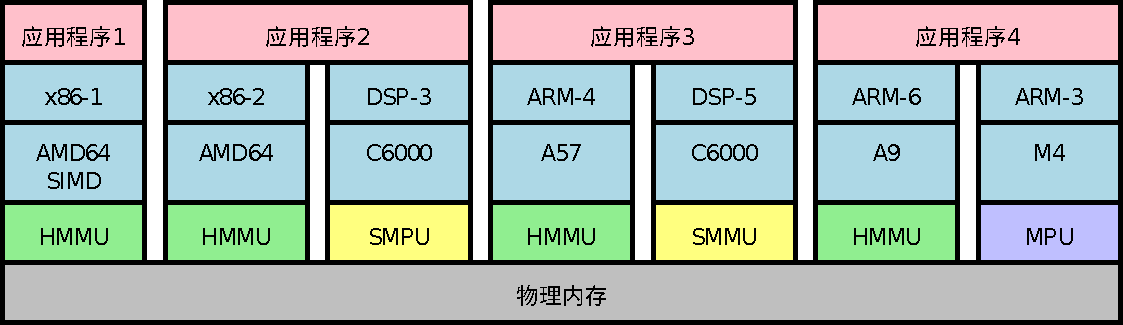
\includegraphics[width=0.72\textwidth]{Figure/image14.pdf}
    \caption{基于异构多核的隔离内核的典型实现方案}
    \label{fig:9-1-heterogeneous-multicore-isolated-kernel}
\end{figure}

\needspace{14\baselineskip}
上图所示为不同架构共同运行的一个例子。在不同的NUMA节点上各运行一个 RME 的实例也是可行的，如下图所示：

\begin{figure}[H]
    \centering
    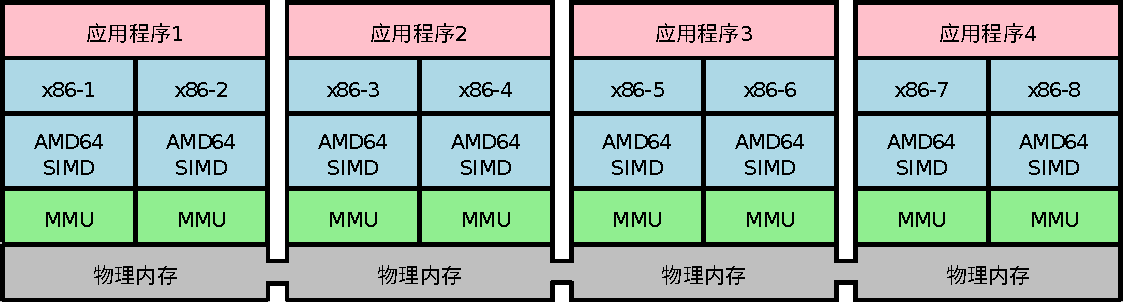
\includegraphics[width=0.72\textwidth]{Figure/image15.pdf}
    \caption{基于NUMA的隔离内核的典型实现方案}
    \label{fig:9-2-numa-isolated-kernel}
\end{figure}

\subsection{无节拍内核的实现}\label{subsec:9-tickless-kernel}

无节拍内核要求系统的每个CPU核都具备一个独立可编程的高精度定时器，并且由该高精度定时器产生可变的调度器时间中断。时间片和定时器填充值之间的比例可以由实现者按需自由决定。为了方便实现无节拍内核，系统提供两个函数\_RME\_Tim\_Future和\_RME\_Tim\_Elapse；如果不实现无节拍内核可以不必理会它们。

为了使定时器在潜在的下一超时时点产生中断，在每次当前线程的剩余时间片发生变动后\footnote{如各类中断向量的出口处}都需要将该时间设置成硬件定时器的下一次超时时间。有三种情况可能导致剩余时间片发生变动：（1）由任意原因引起的上下文切换\footnote{也存在上下文切换前后线程的剩余时间片刚好相同的巧合；此时并不需要重编程定时器}，（2）在系统调用向量中使用RME\_SVC\_THD\_TIME\_XFER且当前线程的时间片因此发生改变，（3）发生了定时器中断\footnote{发生这个中断不一定意味着某线程耗尽了自己的时间片，也可能意味着硬件定时器的最长可配置超时时间不够长而需要将一个定时分多段完成}。在某些架构上，重编程定时器耗时可能较久，而发生中断未必一定引起剩余时间片的变动，因此可以自行查询判断进入中断前后的当前线程时间片变动来决定是否需要重编程定时器；定时器中断是一个特例，它肯定需要一次定时器重编程，因而可免去此查询。

内核提供了函数\_RME\_Tim\_Future用于得到该超时时间。如果这段时间的长度超过了硬件定时器能支持的范围，只要将硬件定时器的超时时间设置成允许的最大值即可；RME的设计保证只有实际经过的时间才会从线程剩余时间中抵扣掉，因此不用担心线程剩余时间丢失。

\begin{xltabular}{\textwidth}{@{}>{\hsize=0.5279\hsize\raggedright\arraybackslash}X>{\hsize=1.4721\hsize\raggedright\arraybackslash}X@{}}
\caption{得到最近超时时间片数}\label{tab:9-1-latest-timeout-slices}\\
\toprule
函数原型 & rme\_ptr\_t \_RME\_Tim\_Future(void)\tabularnewline
\endfirsthead
\toprule
函数原型 & rme\_ptr\_t \_RME\_Tim\_Future(void)\tabularnewline
\midrule
\endhead
\bottomrule
\endlastfoot
意义 &
得到距离未来最近一次超时的时间片数，可根据此设置系统定时器的下一次超时时间。\tabularnewline
返回值\strut
 & rme\_ptr\_t

距离未来最近一次超时的时间片数。\strut
\tabularnewline
参数 & 无。\tabularnewline
\end{xltabular}

为了使所有线程消耗的时间都能得到精准的记录，需要在所有可能上下文切换或修改时间片\footnote{除了定时器中断（它会调用\_RME\_Tim\_Handler）以外的各中断向量入口处；严格地讲，如果能够判断本次中断不发生线程切换，也不通过RME\_SVC\_THD\_TIME\_XFER修改当前线程的时间片，则无需调用\_RME\_Tim\_Elapse，但判断线程切换是否发生很困难，且\_RME\_Tim\_Elapse开销很低，因此推荐在所有中断向量的入口处都调用它}的时点前从当前线程中抵扣已消耗的时间。内核为此提供了函数\_RME\_Tim\_Elapse用于记录消耗的时间。

\begin{xltabular}{\textwidth}{@{}>{\hsize=0.5279\hsize\raggedright\arraybackslash}X>{\hsize=1.4721\hsize\raggedright\arraybackslash}X@{}}
\caption{记录时间流逝数}\label{tab:9-2-record-elapsed-time}\\
\toprule
函数原型 & void \_RME\_Tim\_Elapse(rme\_ptr\_t Slice)\tabularnewline
\endfirsthead
\toprule
函数原型 & void \_RME\_Tim\_Elapse(rme\_ptr\_t Slice)\tabularnewline
\midrule
\endhead
\bottomrule
\endlastfoot
意义 &
在发起潜在的上下文切换前记录当前线程已使用的时间片数。\tabularnewline
返回值 & 无。\tabularnewline
参数\strut
 & rme\_ptr\_t Slice

距离上次调用\_RME\_Tim\_Elapse或\_RME\_Tim\_Handler以来经历的时间片数。\strut
\tabularnewline
\end{xltabular}

值得注意的是，虽然无节拍内核的CPU功耗更低，但其实时性未必更好，因为它势必包含在上下文切换前的时间流逝登记，以及在上下文切换后对定时器的重编程。这都可能增加上下文切换临界区的长度，并对系统的实时性产生负面影响。而且，内核向定时器端点发送的信号也将失去周期性，用户态不再能够依赖于它。

在使用无节拍内核时，必须将RME\_TIMESTAMP宏定义为对某个独立的单向自增计数器\footnote{这种计数器通常可以在CPU性能监控单元（Performance Monitoring
  Unit，PMU）或全局计时器中找到；部分架构如x86等也提供专用的、恒常递增（CONSTANT\_TSC）和永不停息（NONSTOP\_TSC）的RDTSC指令}的读取，这可以使时间戳在任何时候都是全局的最新值，从而保证权能操作安定期的安全性。

\subsection{处理器休眠的实现}\label{subsec:9-processor-sleep}

处理器休眠臭名昭著地难以正确实现；漫不经心的设计轻则导致唤醒丢失、系统卡顿，重则导致永久休眠、机器死机。处理器对休眠指令的定义可以分为``瞻前顾后型''、``仅顾后型''和``仅触发型''，三种定义在实现策略上区别很大。如果担心无法正确实现休眠，则可以将其略去。系统的功耗会稍高，这是不休眠的唯一代价。

\subsubsection{``瞻前顾后''型}\label{subsubsec:9-sleep-look-before-and-after}

这是硬件设计最复杂、软件使用最简单的休眠指令定义\footnote{如 ARMv7-M 的设置 SEVONPEND 后的 WFE 指令}。此种休眠指令不论处理器总中断使能与否，行为都完全一致。它（1）在执行前总会原子性地检查是否有中断已经悬起，如果是则将自己当作 NOP 执行，不进入休眠，而（2）在执行后则总会检查当前是否有新的中断悬起或触发，如果是则立刻退出休眠，恢复指令执行。

对于此类型，只需要在休眠时简单地执行休眠指令即可，无需担心中断唤醒丢失。

\subsubsection{``仅顾后''型}\label{subsubsec:9-sleep-after-only}

这是硬件设计和软件使用都较复杂的休眠指令定义\footnote{如某些不标准的 RISC-V 处理器的 WFI 指令；标准的 WFI 指令是``瞻前顾后''型}。此种休眠指令不论处理器总中断使能与否，行为都完全一致。但与``瞻前顾后''型不同，它在执行前不检查是否有中断已经悬起，而是仅在执行后检查当前是否有新的中断悬起或触发，如果是则立刻退出休眠，恢复指令执行。

对于此类型，在关中断下执行则需要警惕中断唤醒丢失问题。如果不做特别处理，而在关闭中断后到在执行休眠指令前有新的中断悬起，这些悬起的中断唤醒就可能会丢失。一个幼稚的做法是，先判别是否有悬起的中断，如果没有再进入休眠：如果判断时没有中断悬起，但新的中断在判断结束后、休眠执行前悬起，该新到中断唤醒一样会丢失。

如果不在乎中断丢失，则只需要在休眠时简单地执行休眠指令即可。如果不能容忍中断丢失，则必须将其作为下一小节所述的``仅触发''型来处理。不过，部分处理器存在配置开关以将休眠指令的行为转换为上一小节所述的``瞻前顾后''型；如果能找到这样的开关，也可以直接打开它。

\subsubsection{``仅触发''型}\label{subsubsec:9-sleep-trigger-only}

这是硬件设计最简单，但软件使用最复杂的休眠指令定义\footnote{如 x86 的 HALT 指令}。此种休眠指令只能在处理器总中断开启时使用，且它一旦使用处理器就立即停止并等待新的中断来临。如果在关中断时误执行了此类指令，则处理器会因为无法接受中断而直接锁死，导致机器永久死机。这给 RME 造成了麻烦：RME 总是在系统调用中断上下文------此时中断必然关闭------中执行休眠指令，因为休眠功能是通过内核功能调用提供的。而 Linux 等宏内核则不存在此问题，因为它们有真正的、开启中断的内核空闲线程来负责休眠。

对于此类型，我们需要伪造一个类似于 Linux``内核线程''的环境来调用休眠指令。具体地：

（1）编写一段代码作为``内核线程''，在其中循环调用休眠指令。它不需要含有任何其它内容，也不需要一个独立的栈。

（2）一旦在 \_RME\_Svc\_Handler 中检测到休眠请求，就用汇编退出中断上下文到该``内核线程''\footnote{而非通常的返回用户态}，且退出到该``内核线程''时要同步开启中断。为此可以现场伪造一个返回栈；该``内核线程''的栈仍使用当前内核栈，同时保存当前内核上下文到当前内核栈上。

（3）当休眠后的首个中断来临时，检测中断打断的是否是``内核线程''。如果是，记录该中断已发生，但暂不运行它的中断向量而是恢复内核上下文，继续完成 \_RME\_Svc\_Handler 的执行。``内核线程''运行结束与否无需关心。

（4）在 \_RME\_Svc\_Handler 运行结束后扫描中断发生记录，运行被推迟的中断向量。最后按照通常的方式返回用户态。

这样一来，休眠指令就在开启中断的前提下被调用，不会导致睡死，而处理器被唤醒后会继续执行之前的内核功能调用，直到该调用处理完毕才会继续处理中断向量，不会在单处理器上导致内核重入。

\subsection{协处理器上下文的保存和恢复}\label{subsec:9-coprocessor-context-switch}

协处理器指浮点处理器、向量处理器等CPU扩展模块，它们也有自己的上下文；无论是否有多个线程共享同一个协处理器，其上下文都必须小心处理，不然除了会造成程序错乱，还会导致协处理器寄存器组变成一个巨大的隐蔽存储通道。这和只关心时间隔离而不关心空间隔离的 RMP 非常不同。此外，RME 中还有一类寄存器状态不受信任的准虚拟化专用线程，这类线程的协处理器需要更加小心处理，因为它报告的协处理器状态也是不受信任的。

掌管协处理器上下文切换的主要函数是\ref{subsubsec:7-coprocessor-register-set-functions}
中介绍的 \_\_RME\_Thd\_Cop\_Swap，它负责在线程上下文切换时一并保存和恢复该协处理器的上下文。协处理器的保存和恢复在它中实现。

根据处理器硬件层面对协处理器控制提供的功能模型，协处理器可以分为``常开型''、``关-开型''、``关-初-用型''和``关-初-净-脏型''，其中每一种都在前一种的基础上提供了更多控制功能以优化其上下文切换性能，其最优切换策略也愈发复杂。当然，每一种类型都可以以性能为代价使用它之前的类型的切换策略；当（1）对信息安全要求非常高、（2）拿不准切换策略应当如何实现、（3）怀疑当前策略实现有误时，可以一律使用``常开''型的切换策略。

\subsubsection{``常开''型}\label{subsubsec:9-coproc-always-on}

这是最简单的协处理器控制模型。在这种模型下，如果硬件层面实现了该协处理器，则它将在硬件上电时永远开启，且不可能关掉，或者软件环境大多默认开启\footnote{如 x86 的 MMX 协处理器；虽然它有开关，但基本属于标配，可以作为``常开''型处理}。此类协处理器只是名义上的协处理器，它甚至可以作为通用寄存器组的一部分进行处理，因此其切换策略是不言自明的：在任何时候都切换该协处理器寄存器组。当然，系统中的一切线程的上下文属性 Attr 都必须含有该协处理器。

在该策略下无需对准虚拟化专用线程进行任何特殊处理。

\subsubsection{``关-开''型}\label{subsubsec:9-coproc-on-off}

这是次简单的协处理器控制模型。在这种模型下，硬件实现了一个在系统启动时默认关闭的协处理器，必须打开该其开关才能使用，否则会产生异常\footnote{如 MIPS 的 COP1 浮点协处理器，它提供一个简单的开关控制位}。此时，可按如下策略切换该协处理器上下文：

首先（1）判断当前线程的上下文属性 Attr\_Cur 是否包括该协处理器；如果包括，则将该协处理器打开并将其上下文保存到当前线程上下文结构体中，如果不包括则什么都不做。然后（2）判断新线程的上下文属性 Attr\_New 是否包括该协处理器；如果包括，则将该协处理器打开并从新线程上下文结构体中恢复上下文到协处理器中，如果不包括则关闭该协处理器。

在该策略下无需对准虚拟化专用线程进行任何特殊处理，除非协处理器的开关状态也由它控制的寄存器报告。由于它报告的协处理器开关状态并不可信，协处理器的最终开关状态应和上下文属性强制保持一致。这一点也适用于后续类型，在下文中不再赘述。

不建议在此类硬件下使用``切换后关闭''-``异常''-``开启''循环策略\footnote{相当多数操作系统采取这种策略}来实现协处理器状态的软件懒保存，因为这种策略会恶化最坏执行时间：首先，所有架构的协处理器都存在大小不等的开关开销，而此策略会增加开关次数；其次，如果两个交替切换的线程都频繁使用协处理器，则每次线程切换都产生一次额外的协处理器开启异常。事实上协处理器状态的保存可以拖到最后一刻------比如新线程要开始使用协处理器之前，或者当前线程的协处理器状态结构体必须更新之前\footnote{那些查询寄存器的内核功能调用可能会读取协处理器状态}------才去做，但这需要记录当前协处理器状态的所属线程并时刻跟踪之，会造成额外的移植者心智负担。只有在平均性能远比最坏执行时间重要时才可以这样做，且在这样做时对处理器微架构的猜测执行（Speculative
execution）机制必须有清晰了解，否则可能引起协处理器状态泄露\footnote{为避免这种情况，官方移植永远不会带着一个线程的协处理器上下文去执行另一个线程，即使协处理器是关闭的}。

不过，使用``初始关闭''-``初次异常''-``永久常开''策略将此类硬件转化为``关-初-脏''型并采取其``切换策略一''则是值得鼓励的，因为异常仅会在线程初次使用协处理器时引发一次。

\subsubsection{``关-初-脏''型}\label{subsubsec:9-coproc-off-initial-dirty}

这是较常见的协处理器控制模型。在这种模型下，硬件不仅实现了协处理器开关，还会实时探测协处理器是否被使用过。如果协处理器未被开启，则使用该协处理器会产生异常；如果协处理器被开启但未被实际访问过，则``脏''位不会被硬件置位，直到该协处理器被第一次实际访问\footnote{如 ARMv7-M 的 FPv4 和 FPv5 浮点处理器}。此时，针对该协处理器的上下文有两种处理策略：

第一种策略将``脏''位当作``初始状态''的象征。它是最常使用的策略，有利于跳过在上下文属性中声明协处理器但从未碰过它\footnote{即便线程的整个生命周期都不使用协处理器也要声明使用，这有利于提高前向兼容性}的线程的不必要的上下文保存和恢复，是 RME 的官方移植中使用的策略；该策略类似于 RMP 采取的策略。该策略的具体操作如下表所示。

\begin{xltabular}{\textwidth}{@{}>{\hsize=0.9261\hsize\raggedright\arraybackslash}X>{\hsize=0.6708\hsize\raggedright\arraybackslash}X>{\hsize=1.4031\hsize\raggedright\arraybackslash}X@{}}
\caption{``关-初-脏''型切换策略一}\label{tab:9-3-off-initial-dirty-strategy-1}\\
\toprule
当前线程 & 新线程 & 操作\tabularnewline
\endfirsthead
\toprule
当前线程 & 新线程 & 操作\tabularnewline
\midrule
\endhead
\bottomrule
\endlastfoot
\multirow{3}{=}{\makecell[l]{不包括协处理器\\（不在Attr中）}} & 不包括协处理器\strut
 & 什么也不需要做\strut
\tabularnewline
& 协处理器没动过 & 开启协处理器\tabularnewline
& 协处理器使用过 &
开启协处理器并从新线程上下文结构体中恢复协处理器上下文\tabularnewline
\multirow{3}{=}{\makecell[l]{协处理器没动过\\（初始）}} & 不包括协处理器\strut
 & 关闭协处理器\strut
\tabularnewline
& 协处理器没动过 & 什么也不需要做\tabularnewline
& 协处理器使用过 &
从新线程上下文结构体中恢复协处理器上下文\tabularnewline
\multirow{3}{=}{\makecell[l]{协处理器使用过\\（脏）}} & 不包括协处理器\strut
 & 先保存协处理器上下文到当前线程上下文结构体，再重新初始化协处理器上下文，最后关闭协处理器\strut
\tabularnewline
& 协处理器没动过 &
保存协处理器上下文到当前线程上下文结构体并重新初始化协处理器上下文\tabularnewline
& 协处理器使用过 &
保存协处理器上下文到当前线程上下文结构体并从新线程上下文结构体中恢复协处理器上下文\tabularnewline
\end{xltabular}

在该策略下需要特别警惕准虚拟化专用线程，因为它报告的``脏''位并不可靠。它可以在修改过协处理器上下文后在用户态清零``脏''位以报告一个伪造的``初始状态''\footnote{这种状况只有存在多核CPU时会发生，其它核可以对该数据结构并行地进行修改}，这样就可以将自己的协处理器状态泄露给新线程。因此，只要当前线程是准虚拟化专用线程，必须无视其``脏''位的状态并认为它使用过协处理器。不过，在它报告自己处于``初始状态''时，可以不必保存协处理器上下文到它的上下文结构体；这并不会伤害诚实的准虚拟化专用线程。

第二种策略将``脏''位当作``保存过上下文''的象征。它有利于跳过间歇使用协处理器的线程中不使用协处理器的执行段的不必要的上下文保存，在所有线程都实际使用协处理器时能提高平均性能，但于最坏执行时间并无益处。该策略的具体操作如下表所示。

\begin{xltabular}{\textwidth}{@{}>{\hsize=0.7814\hsize\raggedright\arraybackslash}X>{\hsize=1.0349\hsize\raggedright\arraybackslash}X>{\hsize=1.1837\hsize\raggedright\arraybackslash}X@{}}
\caption{``关-初-脏''型切换策略二}\label{tab:9-4-off-initial-dirty-strategy-2}\\
\toprule
当前线程 & 新线程 &
操作\tabularnewline
\endfirsthead
\toprule
当前线程 & 新线程 &
操作\tabularnewline
\midrule
\endhead
\bottomrule
\endlastfoot
\multirow{2}{=}{\makecell[l]{不包括协处理器\\（不在Attr中）}} & 不包括协处理器\strut
 & 什么也不需要做\strut
\tabularnewline
& 协处理器保存过 &
开启协处理器并从新线程上下文结构体中恢复协处理器上下文\tabularnewline
\multirow{2}{=}{\makecell[l]{协处理器保存过\\（干净）}} & 不包括协处理器\strut
 & 关闭协处理器（并清空协处理器上下文）\strut
\tabularnewline
& 协处理器保存过 &
从新线程上下文结构体中恢复协处理器上下文\tabularnewline
\multirow{2}{=}{\makecell[l]{协处理器未保存\\（脏）}} & 不包括协处理器\strut
 & 先保存协处理器上下文到当前线程上下文结构体，再清零当前线程的``脏''位，最后关闭协处理器（并清空协处理器上下文）\strut
\tabularnewline
& 协处理器保存过 &
先保存协处理器上下文到当前线程上下文结构体，再清零当前线程的``脏''位，最后从新线程上下文结构体中恢复协处理器上下文\tabularnewline
\end{xltabular}

在该策略下无需对准虚拟化专用线程进行任何特殊处理\footnote{在该策略下，新线程的``脏''位必定是清零的}。即便它报告的``脏''位的状态并不可信，在切换到它时协处理器上下文也总是被重新装载，不可能通过恶意操纵此位将自己的上下文泄露出去。

注：理论上讲，操作系统可以在线程上下文结构体中引入一个额外的变量来记录``初始''状态，该状态用来单独指示线程是否曾碰过协处理器，这样就可以将``关-初-脏''型转化为下一小节所述的``关-初-净-脏''型以进一步提升性能。但是，这会引入额外的复杂性和内存消耗，且引入该变量会给代码读者造成额外的心智负担，因此 RME 的官方移植不采取这种方案。

\subsubsection{``关-初-净-脏''型}\label{subsubsec:9-coproc-off-initial-clean-dirty}

这是最先进也最复杂的协处理器控制模型，它为协处理器的所有状态都提供了原生的独立指示，因此可以获得最好的性能。如果协处理器未被开启，则使用该协处理器会产生异常；如果协处理器被开启但未被实际访问过，则协处理器会停留在``初始''状态，直到该协处理器被第一次实际访问\footnote{如RISC-V的 F、D 和 Q 标准扩展}，此时硬件会使协处理器会进入``脏''状态；在线程切换的协处理器上下文保存结束后，软件并不会把``脏''状态修改为``初始''状态，而是修改为``干净''状态；在``干净''状态下的任何协处理器访问也会导致硬件把协处理器变为``脏''状态。其切换策略如下表所示：

\begin{xltabular}{\textwidth}{@{}>{\hsize=0.7464\hsize\raggedright\arraybackslash}X>{\hsize=1.0405\hsize\raggedright\arraybackslash}X>{\hsize=1.2131\hsize\raggedright\arraybackslash}X@{}}
\caption{``关-初-净-脏''型切换策略}\label{tab:9-5-off-initial-clean-dirty-strategy}\\
\toprule
当前线程 & 新线程 &
操作\tabularnewline
\endfirsthead
\toprule
当前线程 & 新线程 &
操作\tabularnewline
\midrule
\endhead
\bottomrule
\endlastfoot
\multirow{3}{=}{\makecell[l]{不包括协处理器\\（不在 Attr 中）}} & 不包括协处理器\strut
 & 什么也不需要做\strut
\tabularnewline
& 协处理器没动过 & 开启协处理器\tabularnewline
& 协处理器保存过 &
开启协处理器并从新线程上下文结构体中恢复协处理器上下文\tabularnewline
\multirow{3}{=}{\makecell[l]{协处理器没动过\\（初始）}} & 不包括协处理器\strut
 & 关闭协处理器\strut
\tabularnewline
& 协处理器没动过 & 什么也不需要做\tabularnewline
& 协处理器保存过 &
从新线程上下文结构体中恢复协处理器上下文\tabularnewline
\multirow{3}{=}{\makecell[l]{协处理器保存过\\（干净）}} & 不包括协处理器\strut
 & 重新初始化协处理器上下文并关闭协处理器\strut
\tabularnewline
& 协处理器没动过 & 重新初始化协处理器上下文\tabularnewline
& 协处理器保存过 &
从新线程上下文结构体中恢复协处理器上下文\tabularnewline
\multirow{3}{=}{\makecell[l]{协处理器未保存\\（脏）}} & 不包括协处理器\strut
 & 先保存协处理器上下文到当前线程上下文结构体，再将当前线程转变为``干净''状态，再重新初始化协处理器上下文，最后关闭协处理器\strut
\tabularnewline
& 协处理器没动过 &
先保存协处理器上下文到当前线程上下文结构体，再将当前线程转变为``干净''状态，最后重新初始化协处理器上下文\tabularnewline
& 协处理器保存过 &
先保存协处理器上下文到当前线程上下文结构体，再将当前线程转变为``干净''状态，最后从新线程上下文结构体中恢复协处理器上下文\tabularnewline
\end{xltabular}

在该策略下需要特别警惕准虚拟化专用线程，因为它报告的任何协处理器状态都不可靠\footnote{在该策略下，新线程不可能处于``脏''状态}。它可以在修改过协处理器上下文后在用户态修改协处理器状态寄存器以报告一个伪造的``初始''状态，这样就可以将自己的协处理器状态泄露给新线程。因此，只要当前线程是准虚拟化专用线程，必须将其报告的``初始''状态当作``干净''状态来处理。

\subsection{用户态页表直管的实现}\label{subsec:9-user-mode-page-table-management}

虽然 RME 的内核极尽所能地提供了对页表的高效抽象，但出于最坏执行时间可控、用户态灵活性最大化等考虑，RME 的每级页目录都对应于一个权能，页表操作粒度细但效率低。一方面，在一般无需修改页表映射的微控制器场合\footnote{内存保护单元的页表纯粹是软件模拟的，如果不需要修改映射则完全不需要它们}，大量的页目录及其权能会消耗本就不多的系统内存；另一方面，在需要频繁或大量修改页表的微处理器场合\footnote{这一般是出于缺页中断，而缺页中断是实现懒请求的底层手段；在那些在乎平均性能和资源利用率的操作系统（如云计算等）中，懒请求又是一系列效率优化的基础支撑}，页表操作的低效率会拖累整个系统的吞吐率和尾延迟。考虑到不同场景下对内存管理的需求大相径庭，RME 认为内存管理的权责在本质上归于用户\footnote{所有的性能问题在本质上都是权责问题}：用户有责任在需求特殊时自行实现页表管理。

将 RME\_PGT\_RAW\_ENABLE 定义为1即开启用户态页表直管功能。该功能一旦启用，页表的管理即由用户态的可信进程全权控制，该可信进程本质上是内核的一部分\footnote{攻破它和攻破内核的后果完全是一样的，换言之，它属于可信计算基（Trusted
  Computing Base，TCB）}，和内核的区别仅仅在于（1）它表面上运行在用户态，（2）由于前款原因，它可以被抢占，因此不影响系统的最坏执行时间。此时，页表相关的系统调用和底层相关函数会发生一些变化；有关这些变化可参见\ref{subsec:7-general-macro-definitions}
，在此不再赘述。接下来将分两小节阐述极端场景下的用户态页表直管设计。

\subsubsection{深度嵌入式场景}\label{subsubsec:9-deep-embedded-scenario}

深度嵌入式场景中最常用的是微控制器（MCU），其系统的特点是专机专用、实时可靠、预算不多、资源吃紧，其进程一经建立就基本不修改其地址空间映射。此时，除非要实现动态页功能\footnote{部分 RISC-V 微控制器出于成本考虑采用了简化的微架构，不能生成精确的访存越权异常，因而无法使用动态页功能；此时，基本没有不开启用户态页表直管的理由}，保留页目录数据结构及其权能的意义十分有限。

在深度嵌入式场景中，推荐的做法是在工程编译时就生成能够直接填充给内存保护单元（MPU）的表格，并在系统初始化时直接用这些表格初始化MPU以彻底省去内核页表开销；这些表格都是常量，因此可以放在ROM中以进一步削减内存用量。此外，这种方法还可以针对MPU的特性生成配置数据，能比路径压缩页表更好地适配基址-长度型MPU。与 RME 配套的 RVM 虚拟机监视器提供了这一功能；有关如何开启这一功能，请参见 RVM 的手册。

\subsubsection{云原生服务场景}\label{subsubsec:9-cloud-native-scenario}

与深度嵌入式场景相比，云原生服务场景是另一个极端，在其中唱主角的是基于微处理器的标准机架式服务器。它们往往拥有TB量级的内存，因此页表所占的内存空间不值一提。然而，（1）微处理器系统的动态性非常高，进程的创建与销毁、内存的分配与释放十分频繁，由此所致的页表操作都是大开大合的，有时甚至会一次性映射或撤销几十万乃至上百万个页面。如果每次页面映射或撤销都要操作一次页表权能，造成的性能开销将不可忽视。而且，（2）页目录在创建时需要内核将其清零，这会大大拖慢内核的最坏执行时间，如果连续创建多个页目录可能会引入密集的抖动，从而引起尾延迟超标\footnote{在客户端往往表现为程序卡顿、鼠标不跟手，在服务端往往表现为响应波动大、服务质量差}。此外，（3）缺页中断也会引入巨量的页表操作；即便在那些不使用页面交换算法的内存充足的系统上，缺页中断在推迟数据拷贝、按需同步数据方面也有巨大的作用\footnote{如 Linux 的 fork 调用会尽力推迟内存拷贝直到相应的页真的被修改；类似的机制在 mmap 中也存在}，因此对其进行迅捷响应仍十分必要。最后，（4）服务器系统要分配多少内核专用内存难以决定，因此其内核对象登记表 Kotbl 总是覆盖整个内存范围；此时，内核内存与用户内存的动态划界以及内核对象的管理本就需要一个用户态可信进程来包办，再在其中追加一个页表管理功能就再自然不过了。

云原生服务场景中的推荐做法并无一定之规，但总的原则是（1）减少同等页表操作工作量下的IPC的次数，（2）将页表和其它内存对象整合成便于使用的粗粒度实体提供给应用程序，（3）在存在多个管理层次时尽量避免层层加码，以及（4）在设计机制时充分考虑到进程间的时空隔离。当然，如果不频繁操作地址空间或无苛刻的性能要求，不使用用户态页表直管也无甚不妥。

\section{内存保护单元的推荐处理方案}\label{sec:9-mpu-recommendations}

内存保护单元在不同处理器间存在较大的差别。这种差别可分为影响力、区域组织、区域格式三个方面，其应对方式分别在下面三个小节中加以讨论。

\subsection{内存保护单元的影响力}\label{subsec:9-mpu-influence}

此方面的差别在于内存保护单元的区域属性是否对内核态生效。

\subsubsection{全态影响型}\label{subsubsec:9-mpu-all-mode-affecting}

这是最常见的内存保护单元类型\footnote{如 ARMv7-M 等}，它的区域属性既对内核态生效，也对用户态生效。这意味着，如果在陷入内核时不修改区域属性，用户态对某些内存区段的访问控制限制和缓存策略将被施加给内核。一旦内核中的驱动\footnote{RME 不鼓励这样做，但对实时性有极端需求时可能必须将驱动的一小部分写入内核态中断向量}需要访问这些区段，它就可能会受到随机的意外限制\footnote{这取决于在中断向量触发之前打断的是哪个进程}从而导致内核故障。

此时，推荐的做法是在陷入内核之后关闭内存保护单元，并在临出内核之前开启它。不必担心关闭内存保护单元会导致内核故障；此类内存保护单元都具备一个背景区域，当内存保护单元关闭或不包括某区段时，内核态会转而使用该背景区域的访问权限。

RME 的所有官方移植均采取临时关闭内存保护单元的做法。这意味着，内核运行时总是使用背景区域，其访问权限与缓存策略和内存保护单元未开启时一致；这非常有利于裸机驱动中中断向量的移植。

\subsubsection{仅用户态型}\label{subsubsec:9-mpu-user-mode-only}

这是次常见的内存保护单元类型，它的各区域可以配置为仅对用户态生效。一旦陷入内核，一切访存便不受它限制。

此时，无需进行任何特殊处理就可以得到理想的行为。

\subsection{内存保护单元的区域组织}\label{subsec:9-mpu-region-organization}

此方面的差别在于内存保护单元是否针对不同类型内存准备了不同的区域。

\subsubsection{统一型}\label{subsubsec:9-mpu-unified}

绝大多数处理器采取这种设计，它的任何一个条目都可以指定给任意类型的内存区段。

此时，无需进行任何特殊处理就可以得到理想的行为。

\subsubsection{独立型}\label{subsubsec:9-mpu-separate}

少数处理器采取这种设计，它的条目分为代码、数据和设备三个部分，每个部分有一定数量的专用条目。

RME 和 RVM 当前并不支持这种设计，RME 也不提供相应的官方移植。事实上，RME 支持或计划支持的微控制器架构中不包含独立型设计。

\subsection{内存保护单元的区域格式}\label{subsec:9-mpu-region-format}

此方面的差别在于内存保护单元中各个区域的格式。

\subsubsection{次方型}\label{subsubsec:9-mpu-power-of-two}

这是最常见的内存保护单元区域格式\footnote{如 ARMv7-M 等}。该格式规定，每一个区域对应的内存区段长度必须是2的次方，而且该内存区段的起始地址必须对齐到这个2的次方。部分设计还允许将一个区段等分成4、8或16个独立的子区域，每个子区域都可以被选择性地打开或关闭。

这种区域格式与页式内存管理单元的``页''接近，因此可将这些区域看作软件填充的 TLB。RME 内置的路径压缩页表算法可以很好地应对这种格式。

\subsubsection{连续型}\label{subsubsec:9-mpu-contiguous}

这是次常见的内存保护单元区域格式\footnote{如 ARMv8-M 等}。该格式规定，每一个区域都可以指定一个任意的起始地址和结束地址，只要这些地址对齐到处理器字长即可。

这种区域格式与段式内存管理单元的``段''接近，因此 RME 内置的路径压缩页表算法和它不甚匹配。因此，在进行移植时，推荐将连续的页面映射合并为同一个区域中；为了方便内核进行此种合并，用户态要有意地按地址先后顺序映射连续的页面。

\subsubsection{可变型}\label{subsubsec:9-mpu-variable}

这是最不常见的内存保护单元区域格式\footnote{如 RISC-V 等}。该格式规定，每一个逻辑区域都可以是次方型或连续型：当该逻辑区域是次方型时，它占据一个物理区域；而当该逻辑区域是连续型时，它占据两个物理区域。总的物理区域的数量是有限的。

这种区域格式非常灵活，因此在设计元数据缓存时必须非常小心。为了尽最大可能提升物理区域的利用率，在加入连续的页面时可考虑将三个以上的次方型逻辑区域合并为一个连续型逻辑区域；这种合并在加入动态页时可能也必须执行。为了方便内核进行此种合并，用户态要有意地按地址先后顺序映射连续的页面。

\section{RME中多核可扩展性的限制因素}\label{sec:9-multicore-scalability-limits}

在 RME 中，并非所有的操作都可以互不影响地执行。典型的不能这样执行的操作是多个CPU试图同时向一块内存中创建内核对象。下面列出不能并行执行的操作，并且说明其原因。

\subsection{RME\_TIMESTAMP的更新}\label{subsec:9-timestamp-update}

如果 RME\_TIMESTAMP 被定义为一个变量，则它的更新必须由一个而非多个处理器完成。在多核处理器上，需要其它核同步这个变量到自己的缓存行。因此，这个操作是不能很好并行化的。但是这并不会对系统的并行度有很大影响，因为大型系统的时钟中断频率可以被配置的较低。

如果RME\_TIMESTAMP被定义为对某个自由递增计数器\footnote{如x86的 RDTSC 等}的读取，则没有此问题。值得注意的是多封装系统：虽然同一个物理CPU封装内部的核心的计数器可能是一致的，但不同物理CPU封装之间的计数器可能会产生不一致。在这种情况下，需要移植者自行解决该问题。

\subsection{多核同时在一段内核内存区域创建内核对象}\label{subsec:9-concurrent-kernel-object-creation}

由于对内核对象的创建都要写入内核对象登记表，因此当多个CPU试图竞争地写入表的同一个位置的时候，就会发生大量的缓存行更新而使得这个操作不能很好地并行化。

\subsection{多核同时向某信号端点发送信号}\label{subsec:9-concurrent-signal-sending}

由于这是一个原子比较交换操作，CPU和总线控制器可能会在硬件层面锁总线，因此多核同时累加实际上是串行完成的。因此，这种情况不能很好地并行化。当然，如果系统具备可以并行进行累加的硬件\footnote{常见的现代架构一般都具备此类硬件}，则这个问题不存在。

\subsection{多核同时进行同一个根权能的权能传递或移除}\label{subsec:9-concurrent-root-capability-transfer}

由于权能的引用计数是保存在根权能内部的，因此多个针对同一根权能同时进行的权能传递或移除会同时修改引用计数。这会引发大量的缓存行更新而使得这个操作不能很好地并行化。但是，这个问题一般在系统中并不存在，这一是因为权能的传递往往相对而言是很少进行的操作，二是因为在多核系统中用户程序往往会为每个核创建其专有内核对象。

由于内核内存权能（RME\_CAP\_TYPE\_KOM）和内核功能调用权能（RME\_CAP\_TYPE\_KFN）的根权能仅在系统启动时被创建，因此系统中任何的这两种叶权能都必然来自启动时创建的、不能被删除的初始权能。幸运的是，这两种权能都没有内核对象，也不会被任何其他内核对象引用，因此 RME 对它们做了特殊优化：它们不会记录自己的根权能，也不会进行引用计数，这样就避免了此问题。

\section{RME在32位系统中的限制因素}\label{sec:9-32bit-limitations}

RME 在32位处理器的情况下，受限于处理器字长长度，对某些功能的实现有所制约。被制约的两个功能是线程创建和安定时间的计算。

\subsection{线程的线程号}\label{subsec:9-thread-id}

RME 中每个线程在绑定时都对应一个TID，它的长度是半个机器字长。因此，在32位系统上一共仅有2\textsuperscript{16}个不同的TID\footnote{在64位系统中该值为2\textsuperscript{32}，因此不是问题}。如果要创建多于这个数量的线程，那么就意味着在绑定时某些线程的TID必然要重合。如果用户态软件设计的时候没有考虑这一情况，那么就会造成麻烦。

不过，在一般的32位系统中这不是个问题。在现代语境下，32位系统主要是嵌入式系统，因此线程的数量一般很少。在这个前提下，用户态总是可以找一个没有使用的TID分配给新的线程。

\subsection{安定时间的计算}\label{subsec:9-quiescence-time}

系统中所有的安定时间都是通过与 RME\_TIMESTAMP 的值相比较而计算得出的。该值随着每个时钟嘀嗒自增。RME\_TIMESTAMP 的长度总是一个机器字长，因此会存在溢出回滚的问题。
比如，在该值为0x00000000的时候，有一个操作发生\footnote{如权能冻结}，需要10个时间片的安定时间，那么等待到 RME\_TIMESTAMP 的值超过0x0000000B或更高的时候，就可以对该权能进行下一步操作了。但是，如果我们经过很长一段时间没有做下一步操作，而是等待到该计数器计时到尽头返回0值时再进行下一步操作，我们会发现该位置又进入不安定的状态：其实该位置早已安定，这种不安定是变量溢出导致的假象。

因此，在32位多核系统下，如果发现经过了安定时间以后对象不安定，那么可以隔一个安定时间以后立即再试一次，直到成功为止。在64位系统下由于 RME\_TIMESTAMP 永不溢出，因此该问题是不会发生的。

\section{RME中已知的潜在隐蔽通道}\label{sec:9-known-covert-channels}

在 RME 中有一些已知的潜在隐蔽通道。这些隐蔽通道包括两种，如下列出。

\subsection{隐蔽存储通道}\label{subsec:9-covert-storage-channel}

RME 中存在的隐蔽存储通道主要发生在共享权能、内核对象和权能表的两个进程之间。对于共享权能或内核对象的情况，两个进程可以通过对该权能或内核对象的操作试探和改变它们的状态，从而完成信息传递。

此外，在具备协处理器的系统中，如果协处理器上下文保存和恢复的部分实现不当，可能导致协处理器寄存器组被当做一个带宽很大的隐蔽存储通道使用。在那些实现惰性协处理器寄存器组内容保存和恢复的场合，即便实现正确，也可能导致恶意任务能够推测其它敏感任务对协处理器的使用状况\footnote{CVE-2018-3665}，或者将它当成一个定时通道使用。出于这个原因，在 RME 的所有默认实现中，线程的正在使用的协处理器寄存器组总是会在切换时立刻被保存和恢复。

内核功能调用实现不当也存在同样的问题，在设计上也需要慎重处置。

\subsection{隐蔽定时通道}\label{subsec:9-covert-timing-channel}

在 RME 中，时间片和调度是由用户管理的，因此如果用户的调度算法或时间片分配算法编写不当，会导致大量隐蔽定时通道的出现。为了减少这种通道的带宽，可以考虑禁用处理器的用户态高精度计时器指令\footnote{如 x86 的 RDTSC}。关于此部分，请自行查阅相关资料，在此不做详细说明。

\section{内存一致性模型}\label{sec:9-memory-consistency-model}

RME 大量地使用了无锁数据结构，因此内存一致性模型显得至关重要。内存一致性模型总的而言可以分为两类：强顺序一致性模型和弱一致性模型。在强顺序一致性模型中，多核处理器上的所有内存访问有一个全局顺序，也即在所有的处理器看来，其他处理器对内存的操作顺序都总是一致的；在弱一致性模型中，一个处理器观察到的其他处理器的操作可能发生乱序，而且如果两个处理器都同时观察第三个处理器，观察到的乱序也可能是不一样的。

在一个弱一致性模型的处理器中，可能发生如下四种乱序：

读-读乱序，也即两个相邻的读操作之间没有一定顺序。

读-写乱序，也即一个相邻的读-写对之间没有一定顺序。

写-读乱序，也即一个相邻的写-读对之间没有一定顺序。

写-写乱序，也即两个相邻的写操作之间没有一定顺序。

实际上，在两种一致性模型之间是一个连续的光谱。某些处理器可能对写-读是乱序的，但对其他情况则是顺序的\footnote{比如 x86-64}。

乱序可能导致某些同步标志失效。通常而言，一个共享内存区域都有一个同步标志把守，同步标志的值代表了共享内存区当前的状态。我们先检查并且尝试占有该同步标志，然后再在共享内存区域中进行操作；当操作完成后，我们先把工作收尾，然后再释放该标志位。当乱序发生时，共享内存区域内部的操作可能在占有该同步标志之前就发生了，而收尾工作则有可能拖到同步标志被释放之后。这都破坏了临界区域的性质。因此，在获取标志之后应当加上一个内存屏障，保证对共享内存的操作必须在标志被获取后才开始；在收尾工作之后应当加上一个内存屏障，保证同步标志的释放在收尾工作结束后才进行。虽然 RME 并不使用上面所述的锁来进行内核同步，但是内存一致性仍然会影响内核的同步操作。

为了消除内存重排序对内核的影响，RME 提供了两个宏 RME\_READ\_ACQUIRE() 和 RME\_WRITE\_RELEASE() 来进行内存操作同步。并且，比较交换原子操作都要求在最后附加一个完全内存屏障。关于具体的实现指导，请参见\ref{sec:7-processor-special-function-macro-porting}
所述。

\section{RME中已知的影响实时性的因素}\label{sec:9-realtime-influencing-factors}

在RME中已知的影响实时性的主要因素有两个，分别是权能表和页表。

\subsection{过长的权能表}\label{subsec:9-long-capability-table}

权能表对实时性的影响主要表现在权能表的创建和删除上。由于 RME 并没有采取内核抢占点的实现，因此权能表在创建和删除时会一次性连续访问大量的内存。如果创建的权能表的大小比较大，而内核中 RME\_CPT\_ENTRY\_MAX\footnote{见第~\ref{subsec:7-general-macro-definitions}~节}又未加限制而不能阻止创建时，就会发生内核短暂失去响应的情况。要避免这种情况，需要设置RME\_CPT\_ENTRY\_MAX以限制权能表的最大大小，或仅允许受信任的用户态根权能管理器在不需要响应实时中断的处理器核上创建和删除权能表。

\subsection{缺页中断}\label{subsec:9-page-faults}

对于\ref{subsubsec:8-single-core-mpu}
所述的页表实现，动态页可能会产生缺页中断\footnote{但静态页永远不会}，从而无法保证对动态页数据访问的实时性；对于\ref{subsubsec:8-software-filled-mmu}
和\ref{subsubsec:8-software-filled-mmu}
所述的页表实现，如果映射的静态页的数量超过了硬件支持的区域数量，那么甚至在静态页上也会引起缺页中断。在这种状况下一个解决办法是不要映射过多的静态页。

对于\ref{subsubsec:8-hardware-filled-mmu}
所述的页表实现，由于快表由硬件填充，因而具有更大的不确定性。如果需要在硬件填充的内存管理单元上获取实时性能，推荐使用支持快表锁定的处理器，这样就可以将实时进程的页面锁定在快表中\footnote{这是推荐的做法}；如果处理器不支持快表锁定，在映射页面时可以采用快表着色算法，尽量使得实时进程的快表条目不会被非实时进程挤占，或者使得系统中映射的总页面数量不超过快表的大小\footnote{这是次好的做法}；如果处理器连快表着色算法都无法实现，还可以着色数据缓存而使实时进程的页表的一部分永存于数据缓存中，一旦发生快表不命中，可以使查找速度大大加快\footnote{这是最坏的做法}。

\subsection{链接读/条件写造成的活锁}\label{subsec:9-ll-sc-livelock}

在很多处理器中，除了链接读（Linked Load，LL）和条件写（Store
Conditional，SC）之外就没有提供其他的原子指令了。虽然这两条指令在语义上足够灵活，可以实现几乎所有的原子操作，但它们可能导致活锁，从而导致 RME 提供的实时性保证和权能安定保证失效。因此，在使用这对指令时必须注意：

\begin{enumerate}
\def\labelenumi{\arabic{enumi}.}
\item
  如果处理器提供了LL/SC的免饥饿保证，使用它们实现 RME 的所有原子操作不会引发问题。
\item
  如果处理器未提供LL/SC的免饥饿保证，但提供了专用的原子操作指令\footnote{如 CMPXCHG、XADD、AMOADD、AMOAND 等}，此时应避免使用LL/SC而改用专用原子指令。
\item
  如果处理器未提供LL/SC的免饥饿保证，且提供了除 CMPXCHG 之外其余操作的专用原子指令，此时仅应使用LL/SC实现 CMPXCHG，其它指令则改用专用的原子操作，而且在实现 CMPXCHG 时，一旦循环尝试次数超过某个阈值就退出，从而达成免饥饿性质。虽然这变更了 CMPXCHG 的语义，使其在合乎成功条件时依然有几率失败，但好过无限的活锁循环。RME 的设计能够接受这种变造的 CMPXCHG 语义。
\item
  如果处理器未提供LL/SC之外的任何原子指令，且 LL/SC 无免饥饿保证，则推荐限制系统中CPU的数量，如双核或四核。这样一来，由于系统调用存在一个很大的固有开销，CPU间在系统调用中的竞争程度就是可控的，从而变相达成免饥饿。事实上，现代多核处理器普遍满足情况1-3，因此情况4很罕见。
\end{enumerate}

\section{RME对C语言标准和MISRA标准的背离}\label{sec:9-c-and-misra-deviations}

\subsection{C未定义行为：类型双关指针别名可以存在并不遵循严格别名机制}\label{subsec:9-type-punning-aliasing}

类型双关（Type-Punning）指针别名（Pointer-Aliasing）是一种广泛存在于 C 语言\footnote{指 C90，下同}实际应用中的用法，它允许两个不同类型的指针引用同一块内存。这在网络协议栈中是非常常见的，因为我们往往需要组装或者拆解网络封包，变换其字节序，等等。在操作系统中这也很常见，尤其是将无符号整数指针与结构体指针来回转换以方便对对象的操作。不幸的是，C 语言的严格别名机制（Strict
Aliasing
Rule）并不允许两个不同类型的指针引用同一块内存，除非是兼容类型或者从其他类型转换到 char\hyperref[cite:9-2]{{[}2{]}}，而且也没有通用的办法绕开这一点。通常而言有三种方法可以避免类型双关，它们分别是：

\begin{enumerate}
\def\labelenumi{\arabic{enumi}.}
\item
  使用 union 来进行不同类别之间的转换。不幸的是这在 C 中是被定义行为而在 C++中不是，而 RME 的代码由于可能和使用 C++写成的某些库直接链接\footnote{如果不希望使用 \texttt{extern "C"} 的话}而需要作为 C++被编译，因此仍然有可能是未定义行为。此外，此种方法对长度在编译时不确定的数组对象是束手无策的，除非牺牲潜在的性能来对它们进行逐一转换。最后，这样使用 union 不符合 union 的设计精神，属于对语言规则的滥用。
\item
  使用 char* 来进行操作。不幸的是现存编译器对这一点的优化非常糟糕；某些相当优秀的编译器甚至也会把这些操作编译成逐字节访问的指令，对于低质量嵌入式编译器则更是如此。因此，这是一种不好的解决方案。
\item
  使用 memcpy 函数在两个不兼容的指针间拷贝内容，操作完后再拷贝回去，寄希望于编译器能够探测这种行为并且优化掉重复的 memcpy。这巧妙地利用了 memcpy 的参数为 char*，而 char*总是可以和任何指针别名的特点。它带来的直接问题是，某些低质量编译器可能不够智能，有时不会把 memcpy 函数优化掉，而导致生成的代码中实际调用了两次 memcpy，从而导致巨大的性能损失。而且一旦 memcpy 没有被优化掉，这可能会导致在函数内部声明的局部拷贝缓冲区被分配在栈上，大大增加栈消耗而导致堆栈溢出。最后，此类对 memcpy 的使用是不符合 memcpy 的设计意图的，属于对语言漏洞的滥用；C 标准对此种做法不持鼓励态度。

  有鉴于以上三种方法的问题，RME 并不使用这些方法，而是直接使用类型双关指针别名，而在编译时关掉相关的优化\footnote{如 GCC 的-fno-strict-aliasing 选项}。
\end{enumerate}

\subsection{C未定义行为：一个字节的长度总是8位，一个char类型的长度总是一个字节}\label{subsec:9-char-size-eight-bits}

C 语言并未定义 char 的长度，它仅仅表示 char 必须等于系统中基本字符集的单个字符的宽度\hyperref[cite:9-2]{{[}2{]}}，理论上讲一个 char 类型可以是32或16个二进制位\footnote{早期的某些嵌入式编译器会这样做}。现时的所有主流编译器和架构上 char 的长度都总是8个二进制位，因此我们在代码中也作此假设以避免不必要的``char 类型长度''配置宏。

\subsection{C未定义行为：指针的实际表示总是机器可直接识别的地址}\label{subsec:9-pointer-representation}

C 语言并未定义指针在内存中应该如何表示。理论上讲，指针变量的实际表示可以是任何东西，只要在解引用时它返回的值是按照 C 语言语义指向的变量的值就可以了\hyperref[cite:9-2]{{[}2{]}}。这使得在严格的 C 标准下将指针对齐到某个内存粒度是不可能的，因为无法对其使用掩码来掩蔽掉它的某些位；也无法利用指针的某些不使用的位来存储其他信息。因此，我们假设指针的实际表示总是机器可直接识别的二进制地址，这一点在所有 RME 支持或计划支持的架构上都是成立的。

\subsection{C未定义行为：指针的长度总是小于或等于一个机器字长}\label{subsec:9-pointer-size-bound}

C 语言并未规定指针的长度。指针的长度可以是任何值，只要按照 C 语言的语义，它能够正常工作即可。完全有可能出现指针的长度比一个机器字长长从而无法放置在长度等于一个机器字长的无符号整数值内部的情况\hyperref[cite:9-2]{{[}2{]}}。这种情况现时仅仅出现在几乎所有的8位单片机和部分16位单片机上，而 RME 从设计之初就不打算支持这些架构，因此我们可以假设指针的长度总是小于或等于一个机器字长。实际上，在 RME 支持或计划支持的所有架构上，指针的长度都总是等于一个机器字长。此外，我们不使用 C 库提供的 uintptr\_t 等类型，因为这些类型只有 C99 才有，而且甚至是可选实现的。

\subsection{C未定义行为：强制转换指针到一个机器字长的无符号整数值总是不改变它的实际表示}\label{subsec:9-pointer-integer-cast}

C语言并未规定指针在转换到无符号整数后，其实际表示应如何变化。它只规定了，如果先把一个指针转换成一个空间足够大的无符号整数后再转换回去，来回转换后得到的指针在和原指针做比较操作时应当视为相等\footnote{这甚至不禁止转换前和来回转换后得到的表示有差异，只要这两个值在做指针比较时总是按照相等处理即可}\hyperref[cite:9-2]{{[}2{]}}。如果指针在转换到无符号整数后的表示会变化，那么我们会遇到与\ref{subsec:9-pointer-representation}
所述类似的问题。因此，我们假设强制转换指针到一个机器字长的无符号整数值总是不改变它的实际表示，这一点在所有RME支持或计划支持的架构上都是成立的。

\subsection{C未定义行为：外部标识符的长度扩展为31字符}\label{subsec:9-external-identifier-length}

C90 规定外部（extern）变量名最少只有前 6 个字符是有效的。这对任何操作系统来说都太少了。因此，RME 把这个限制放宽到了与内部变量名限制相同的31个字符。所有的现代编译器均支持这一点。

\subsection{C 未定义行为：对非 volatile 变量的修改总是被保留}\label{subsec:9-nonvolatile-write-preserved}

最新的C23规定对非 volatile 变量的写操作不再是一个必须被保留的副作用\footnote{它在 C17 及以前曾经是}。此时，如果编译器确认对某个数据结构的写操作不会被``同一线程''内的任何读操作读到，该写操作可以被优化掉。比如，足够聪明的链接时优化（Link-Time
  Optimization，LTO）编译器可能会误认为内核对象的创建操作是多余的，因为该对象在创建后就不在被当前系统调用读取了，因此实际的创建操作可以被优化掉。这个优化无法被编译器屏障关闭，因为编译器屏障只能强迫编译器与内存同步那些必要变量的状态，但并不能阻止编译器认为某些写操作是无用的。幸运的是，这种理论上可行的优化在现实中并不存在，因为（1）对实用编译器作者而言，分析全局变量写操作副作用的无效性是困难和危险的，费力而不讨好，（2）对程序员而言，它强迫一切全局变量写访问以 volatile 指针的形式进行\footnote{如果这些全局变量没有以 volatile 声明的话}，使编程非常繁琐。鉴于很多流行的操作系统都假设写操作会被保留\footnote{如 Linux 等}，而用于编译这些流行操作系统的编译器也不进行这一优化，我们也作此假设。

\subsection{MISRA-C背离情况说明}\label{subsec:9-misra-c-deviations}

RME 对于 MISRA-C:2012\hyperref[cite:9-3]{{[}3{]}}中的所有三类建议都进行了严格检查，并且所有的背离都被批准。

RME 对于 MISRA-C:2012\hyperref[cite:9-3]{{[}3{]}}中所述的强制（Mandatory）类别没有任何背离发生。

RME 对于 MISRA-C:2012\hyperref[cite:9-3]{{[}3{]}}中所述的要求（Required）类别的背离如下：

\begin{xltabular}{\textwidth}{@{}>{\hsize=0.5279\hsize\raggedright\arraybackslash}X>{\hsize=1.4721\hsize\raggedright\arraybackslash}X@{}}
\caption{RME对MISRA-C:2012中所述的要求（Required）部分的背离}\label{tab:9-6-misra-required-deviations}\\
\toprule
条目 & 解释\tabularnewline
\endfirsthead
\toprule
条目 & 解释\tabularnewline
\midrule
\endhead
\bottomrule
\endlastfoot
1.3 &
某些如前所述的未定义行为对于实现操作系统这样的底层软件而言是必需的。\tabularnewline
5.1 &
RME 扩展了外部标识符的有效长度到31位。这对于操作系统的软件工程而言是必需的。\tabularnewline
11.3 &
类型双关指针别名对于操作系统这样的软件而言是必需的。RME 事实上仅在结构体和子结构体处使用此类双关指针别名。\tabularnewline
11.9 & RME 不使用 NULL 而使用 RME\_NULL。这是一个非常细微的不一致。\tabularnewline
14.3 &
RME在检查配置是否正确的流程中大量使用了编译时就能确定结果的布尔表达式。这些布尔表达式都被直接送入 RME\_ASSERT 宏，确保 RME 被正确配置。这提高了软件的质量。\tabularnewline
\end{xltabular}

\needspace{20\baselineskip}
RME 对于 MISRA-C:2012\hyperref[cite:9-3]{{[}3{]}}中所述建议（Advisory）类别的背离如下：

\begin{xltabular}{\textwidth}{@{}>{\hsize=0.5279\hsize\raggedright\arraybackslash}X>{\hsize=1.4721\hsize\raggedright\arraybackslash}X@{}}
\caption{RME对MISRA-C:2012中所述的建议（Advisory）部分的背离}\label{tab:9-7-misra-advisory-deviations}\\
\toprule
条目 & 解释\tabularnewline
\endfirsthead
\toprule
条目 & 解释\tabularnewline
\midrule
\endhead
\bottomrule
\endlastfoot
2.5 &
在硬件抽象层，尤其是固件库中，某些宏是作为配置选项出现的。它们可能在当前配置中没有使用，但必须保留以适应未来的软件配置调整，有利于维护工程的一致性和提高代码质量。这些宏都有很好的注释和文档可供参考。\tabularnewline
2.7 &
由于 RME 的硬件抽象层要对所有的受支持硬件定义统一的接口，因此不免会有一些硬件抽象层函数的参数对于某些架构而言是多余的。\tabularnewline
11.4 &
转换一个无符号数到指针对于操作系统这样的软件而言是必需的。\tabularnewline
12.4 &
在32位系统上RME\_TIMESTAMP可能会在自增时溢出并重新从0开始，这是正确的实现。在\ref{subsec:9-quiescence-time}
中有关于它的详细的解释。\tabularnewline
15.4 &
RME在内核内存登记表相关代码中有部分循环会有两个 break 都能将其打断，并且在硬件抽象层的页表查询函数中也会有这样的实现。其他形式的实现可能会使实现复杂度增加而不利于工程维护。在出现此种情况的循环中，注释都详细标注了这样做的理由及各个分支的退出条件，并且各个 break 语句均从上到下依次并列。\tabularnewline
15.5 &
基于与 15.4 同样的理由，RME 的一个函数可能会有多个出口。在这些代码处都进行了良好注释，并且其他可选实现会违反其他的要求或建议，并且破坏工程的整体抽象。\tabularnewline
20.5 &
为了使每个函数和变量的声明都只进行一次（包括其 extern 形式），系统性地防止出现隐式声明错误来提高软件质量，RME 使用了独创的分段包含式头文件。该格式要求使用 \#undef。\#undef 仅用于该格式，而且该格式在整个系统中都被良好遵循，也有对应文档进行详细说明。\tabularnewline
\end{xltabular}

\section{术语中英翻译速查表}\label{sec:9-terminology-translation-table}

\begin{xltabular}{\textwidth}{@{}>{\hsize=1.1358\hsize\raggedright\arraybackslash}X>{\hsize=0.8642\hsize\raggedright\arraybackslash}X@{}}
\caption{术语中英翻译速查表}\label{tab:9-8-terminology-translation}\\
\toprule
英文术语 & 中文翻译\tabularnewline
\endfirsthead
\toprule
英文术语 & 中文翻译\tabularnewline
\midrule
\endhead
\bottomrule
\endlastfoot
Capability & 权能\tabularnewline
Component & 组件\tabularnewline
Coroutine & 协程\tabularnewline
Daemon & 守护进程\tabularnewline
Endpoint (Signal) & （信号）端点\tabularnewline
Expandable/Expandability & 可扩展/可扩展性\tabularnewline
Invocation (Thread Migration) & （线程迁移）调用\tabularnewline
Page Directory & 页目录\tabularnewline
Page Entry & 页表项\tabularnewline
Page Table & 页表\tabularnewline
Priority & 优先级\tabularnewline
Process & 进程\tabularnewline
Quiescence & 安定\tabularnewline
Scalable/Scalability & 可伸缩/可伸缩性\tabularnewline
Scheduler & 调度器\tabularnewline
Signal & 信号\tabularnewline
Thread & 线程\tabularnewline
\end{xltabular}

\section{本章参考文献}\label{sec:9-bibliography}

\protect\phantomsection\label{cite:9-1}

\noindent {[}1{]} A. Baumann, P. Barham, P.-E. Dagand, T. Harris, R. Isaacs, S. Peter, et al., ``The multikernel: a new OS architecture for scalable multicore systems,'' in \textit{Proceedings of the ACM SIGOPS 22nd Symposium on Operating Systems Principles}, 2009, pp. 29--44.

\protect\phantomsection\label{cite:9-2}

\noindent {[}2{]} ISO, ``Programming languages---C,'' International Organization for Standardization, ISO/IEC 9899:1990(E), 1990.

\protect\phantomsection\label{cite:9-3}

\noindent {[}3{]} MISRA Association, \textit{MISRA C:2012: Guidelines for the Use of the C Language in Critical Systems}. MIRA, 2013.



\end{document}
